%
% coif3.tex -- coiflet wavelet 3
%
% (c) 2019 Prof Dr Andreas Müller, Hochschule Rapperswil
%
\documentclass[tikz]{standalone}
\usepackage{amsmath}
\usepackage{times}
\usepackage{txfonts}
\usepackage{pgfplots}
\usepackage{csvsimple}
\usetikzlibrary{arrows,intersections,math}
\begin{document}
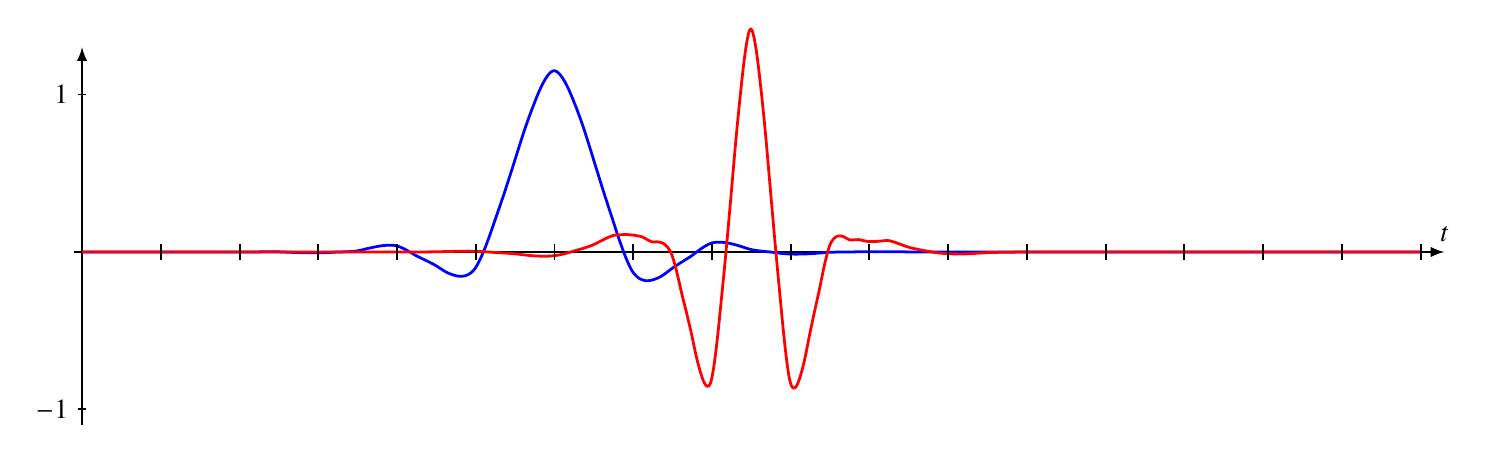
\begin{tikzpicture}[>=latex,yscale=2,xscale=1]

\draw[->,line width=0.7pt] (-0.1,0)--(17.3,0) coordinate[label={$t$}];
\draw[->,line width=0.7pt] (0,-1.1)--(0,1.3);

\draw[line width=1pt,color=blue] (0.00000, -0.00000)
--(0.00195, 0.00000)
--(0.00391, 0.00000)
--(0.00586, -0.00000)
--(0.00781, -0.00000)
--(0.00977, 0.00000)
--(0.01172, 0.00000)
--(0.01367, 0.00000)
--(0.01562, -0.00000)
--(0.01758, -0.00000)
--(0.01953, -0.00000)
--(0.02148, 0.00000)
--(0.02344, 0.00000)
--(0.02539, 0.00000)
--(0.02734, 0.00000)
--(0.02930, -0.00000)
--(0.03125, -0.00000)
--(0.03320, -0.00000)
--(0.03516, -0.00000)
--(0.03711, -0.00000)
--(0.03906, -0.00000)
--(0.04102, -0.00000)
--(0.04297, 0.00000)
--(0.04492, 0.00000)
--(0.04688, 0.00000)
--(0.04883, 0.00000)
--(0.05078, 0.00000)
--(0.05273, 0.00000)
--(0.05469, -0.00000)
--(0.05664, -0.00000)
--(0.05859, -0.00000)
--(0.06055, -0.00000)
--(0.06250, -0.00000)
--(0.06445, -0.00000)
--(0.06641, -0.00000)
--(0.06836, 0.00000)
--(0.07031, 0.00000)
--(0.07227, 0.00000)
--(0.07422, 0.00000)
--(0.07617, 0.00000)
--(0.07812, 0.00000)
--(0.08008, 0.00000)
--(0.08203, 0.00000)
--(0.08398, 0.00000)
--(0.08594, 0.00000)
--(0.08789, 0.00000)
--(0.08984, 0.00000)
--(0.09180, 0.00000)
--(0.09375, 0.00000)
--(0.09570, -0.00000)
--(0.09766, -0.00000)
--(0.09961, -0.00000)
--(0.10156, -0.00000)
--(0.10352, -0.00000)
--(0.10547, -0.00000)
--(0.10742, -0.00000)
--(0.10938, -0.00000)
--(0.11133, -0.00000)
--(0.11328, -0.00000)
--(0.11523, -0.00000)
--(0.11719, -0.00000)
--(0.11914, 0.00000)
--(0.12109, 0.00000)
--(0.12305, 0.00000)
--(0.12500, 0.00000)
--(0.12695, 0.00000)
--(0.12891, 0.00000)
--(0.13086, 0.00000)
--(0.13281, 0.00000)
--(0.13477, 0.00000)
--(0.13672, 0.00000)
--(0.13867, 0.00000)
--(0.14062, 0.00000)
--(0.14258, 0.00000)
--(0.14453, 0.00000)
--(0.14648, 0.00000)
--(0.14844, -0.00000)
--(0.15039, -0.00000)
--(0.15234, -0.00000)
--(0.15430, -0.00000)
--(0.15625, -0.00000)
--(0.15820, -0.00000)
--(0.16016, -0.00000)
--(0.16211, -0.00000)
--(0.16406, -0.00000)
--(0.16602, -0.00000)
--(0.16797, -0.00000)
--(0.16992, -0.00000)
--(0.17188, -0.00000)
--(0.17383, -0.00000)
--(0.17578, -0.00000)
--(0.17773, -0.00000)
--(0.17969, -0.00000)
--(0.18164, -0.00000)
--(0.18359, -0.00000)
--(0.18555, -0.00000)
--(0.18750, -0.00000)
--(0.18945, -0.00000)
--(0.19141, -0.00000)
--(0.19336, -0.00000)
--(0.19531, -0.00000)
--(0.19727, -0.00000)
--(0.19922, -0.00000)
--(0.20117, -0.00000)
--(0.20312, 0.00000)
--(0.20508, 0.00000)
--(0.20703, 0.00000)
--(0.20898, 0.00000)
--(0.21094, 0.00000)
--(0.21289, 0.00000)
--(0.21484, 0.00000)
--(0.21680, 0.00000)
--(0.21875, 0.00000)
--(0.22070, 0.00000)
--(0.22266, 0.00000)
--(0.22461, 0.00000)
--(0.22656, 0.00000)
--(0.22852, 0.00000)
--(0.23047, 0.00000)
--(0.23242, 0.00000)
--(0.23438, 0.00000)
--(0.23633, 0.00000)
--(0.23828, 0.00000)
--(0.24023, 0.00000)
--(0.24219, 0.00000)
--(0.24414, 0.00000)
--(0.24609, 0.00000)
--(0.24805, 0.00000)
--(0.25000, -0.00000)
--(0.25195, -0.00000)
--(0.25391, -0.00000)
--(0.25586, -0.00000)
--(0.25781, -0.00000)
--(0.25977, -0.00000)
--(0.26172, -0.00000)
--(0.26367, -0.00000)
--(0.26562, -0.00000)
--(0.26758, -0.00000)
--(0.26953, -0.00000)
--(0.27148, -0.00000)
--(0.27344, -0.00000)
--(0.27539, -0.00000)
--(0.27734, -0.00000)
--(0.27930, -0.00000)
--(0.28125, -0.00000)
--(0.28320, -0.00000)
--(0.28516, -0.00000)
--(0.28711, -0.00000)
--(0.28906, -0.00000)
--(0.29102, -0.00000)
--(0.29297, -0.00000)
--(0.29492, -0.00000)
--(0.29688, -0.00000)
--(0.29883, -0.00000)
--(0.30078, -0.00000)
--(0.30273, -0.00000)
--(0.30469, -0.00000)
--(0.30664, -0.00000)
--(0.30859, 0.00000)
--(0.31055, 0.00000)
--(0.31250, 0.00000)
--(0.31445, 0.00000)
--(0.31641, 0.00000)
--(0.31836, 0.00000)
--(0.32031, 0.00000)
--(0.32227, 0.00000)
--(0.32422, 0.00000)
--(0.32617, 0.00000)
--(0.32812, 0.00000)
--(0.33008, 0.00000)
--(0.33203, 0.00000)
--(0.33398, 0.00000)
--(0.33594, 0.00000)
--(0.33789, 0.00000)
--(0.33984, 0.00000)
--(0.34180, 0.00000)
--(0.34375, 0.00000)
--(0.34570, 0.00000)
--(0.34766, 0.00000)
--(0.34961, 0.00000)
--(0.35156, 0.00000)
--(0.35352, 0.00000)
--(0.35547, 0.00000)
--(0.35742, 0.00000)
--(0.35938, 0.00000)
--(0.36133, 0.00000)
--(0.36328, 0.00000)
--(0.36523, 0.00000)
--(0.36719, 0.00000)
--(0.36914, 0.00000)
--(0.37109, 0.00000)
--(0.37305, 0.00000)
--(0.37500, 0.00000)
--(0.37695, 0.00000)
--(0.37891, 0.00000)
--(0.38086, 0.00000)
--(0.38281, 0.00000)
--(0.38477, 0.00000)
--(0.38672, 0.00000)
--(0.38867, 0.00000)
--(0.39062, 0.00000)
--(0.39258, 0.00000)
--(0.39453, 0.00000)
--(0.39648, 0.00000)
--(0.39844, 0.00000)
--(0.40039, 0.00000)
--(0.40234, 0.00000)
--(0.40430, 0.00000)
--(0.40625, 0.00000)
--(0.40820, 0.00000)
--(0.41016, 0.00000)
--(0.41211, 0.00000)
--(0.41406, 0.00000)
--(0.41602, -0.00000)
--(0.41797, -0.00000)
--(0.41992, -0.00000)
--(0.42188, -0.00000)
--(0.42383, -0.00000)
--(0.42578, -0.00000)
--(0.42773, -0.00000)
--(0.42969, -0.00000)
--(0.43164, -0.00000)
--(0.43359, -0.00000)
--(0.43555, -0.00000)
--(0.43750, -0.00000)
--(0.43945, -0.00000)
--(0.44141, -0.00000)
--(0.44336, -0.00000)
--(0.44531, -0.00000)
--(0.44727, -0.00000)
--(0.44922, -0.00000)
--(0.45117, -0.00000)
--(0.45312, -0.00000)
--(0.45508, -0.00000)
--(0.45703, -0.00000)
--(0.45898, -0.00000)
--(0.46094, -0.00000)
--(0.46289, -0.00000)
--(0.46484, -0.00000)
--(0.46680, -0.00000)
--(0.46875, -0.00000)
--(0.47070, -0.00000)
--(0.47266, -0.00000)
--(0.47461, -0.00000)
--(0.47656, -0.00000)
--(0.47852, -0.00000)
--(0.48047, -0.00000)
--(0.48242, -0.00000)
--(0.48438, -0.00000)
--(0.48633, -0.00000)
--(0.48828, -0.00000)
--(0.49023, -0.00000)
--(0.49219, -0.00000)
--(0.49414, -0.00000)
--(0.49609, -0.00000)
--(0.49805, -0.00000)
--(0.50000, -0.00000)
--(0.50195, -0.00000)
--(0.50391, -0.00000)
--(0.50586, -0.00000)
--(0.50781, -0.00000)
--(0.50977, -0.00000)
--(0.51172, 0.00000)
--(0.51367, 0.00000)
--(0.51562, 0.00000)
--(0.51758, 0.00000)
--(0.51953, 0.00000)
--(0.52148, 0.00000)
--(0.52344, 0.00000)
--(0.52539, 0.00000)
--(0.52734, 0.00000)
--(0.52930, 0.00000)
--(0.53125, 0.00000)
--(0.53320, 0.00000)
--(0.53516, 0.00000)
--(0.53711, 0.00000)
--(0.53906, 0.00000)
--(0.54102, 0.00000)
--(0.54297, 0.00000)
--(0.54492, 0.00000)
--(0.54688, 0.00000)
--(0.54883, 0.00000)
--(0.55078, 0.00000)
--(0.55273, 0.00000)
--(0.55469, 0.00000)
--(0.55664, 0.00000)
--(0.55859, 0.00000)
--(0.56055, 0.00000)
--(0.56250, 0.00000)
--(0.56445, 0.00000)
--(0.56641, 0.00000)
--(0.56836, 0.00000)
--(0.57031, 0.00000)
--(0.57227, 0.00000)
--(0.57422, 0.00000)
--(0.57617, 0.00000)
--(0.57812, 0.00000)
--(0.58008, 0.00000)
--(0.58203, 0.00000)
--(0.58398, 0.00000)
--(0.58594, 0.00000)
--(0.58789, 0.00000)
--(0.58984, 0.00000)
--(0.59180, 0.00000)
--(0.59375, 0.00000)
--(0.59570, 0.00000)
--(0.59766, 0.00000)
--(0.59961, 0.00000)
--(0.60156, 0.00000)
--(0.60352, 0.00000)
--(0.60547, 0.00000)
--(0.60742, 0.00000)
--(0.60938, 0.00000)
--(0.61133, 0.00000)
--(0.61328, 0.00000)
--(0.61523, 0.00000)
--(0.61719, 0.00000)
--(0.61914, 0.00000)
--(0.62109, 0.00000)
--(0.62305, 0.00000)
--(0.62500, 0.00000)
--(0.62695, 0.00000)
--(0.62891, -0.00000)
--(0.63086, -0.00000)
--(0.63281, -0.00000)
--(0.63477, -0.00000)
--(0.63672, -0.00000)
--(0.63867, -0.00000)
--(0.64062, -0.00000)
--(0.64258, -0.00000)
--(0.64453, -0.00000)
--(0.64648, -0.00000)
--(0.64844, -0.00000)
--(0.65039, -0.00000)
--(0.65234, -0.00000)
--(0.65430, -0.00000)
--(0.65625, -0.00000)
--(0.65820, -0.00000)
--(0.66016, -0.00000)
--(0.66211, -0.00000)
--(0.66406, -0.00000)
--(0.66602, -0.00000)
--(0.66797, -0.00000)
--(0.66992, -0.00000)
--(0.67188, -0.00000)
--(0.67383, -0.00000)
--(0.67578, -0.00000)
--(0.67773, -0.00000)
--(0.67969, -0.00000)
--(0.68164, -0.00000)
--(0.68359, -0.00000)
--(0.68555, -0.00000)
--(0.68750, -0.00000)
--(0.68945, -0.00000)
--(0.69141, -0.00000)
--(0.69336, -0.00000)
--(0.69531, -0.00000)
--(0.69727, -0.00000)
--(0.69922, -0.00000)
--(0.70117, -0.00000)
--(0.70312, -0.00000)
--(0.70508, -0.00000)
--(0.70703, -0.00000)
--(0.70898, -0.00000)
--(0.71094, -0.00000)
--(0.71289, -0.00000)
--(0.71484, -0.00000)
--(0.71680, -0.00000)
--(0.71875, -0.00000)
--(0.72070, -0.00000)
--(0.72266, -0.00000)
--(0.72461, -0.00000)
--(0.72656, -0.00000)
--(0.72852, -0.00000)
--(0.73047, -0.00000)
--(0.73242, -0.00000)
--(0.73438, -0.00000)
--(0.73633, -0.00000)
--(0.73828, -0.00000)
--(0.74023, -0.00000)
--(0.74219, -0.00000)
--(0.74414, -0.00000)
--(0.74609, -0.00000)
--(0.74805, -0.00000)
--(0.75000, -0.00000)
--(0.75195, -0.00000)
--(0.75391, -0.00000)
--(0.75586, -0.00000)
--(0.75781, -0.00000)
--(0.75977, -0.00000)
--(0.76172, -0.00000)
--(0.76367, -0.00000)
--(0.76562, -0.00000)
--(0.76758, -0.00000)
--(0.76953, -0.00000)
--(0.77148, -0.00000)
--(0.77344, -0.00000)
--(0.77539, -0.00000)
--(0.77734, -0.00000)
--(0.77930, -0.00000)
--(0.78125, -0.00000)
--(0.78320, -0.00000)
--(0.78516, -0.00000)
--(0.78711, -0.00000)
--(0.78906, -0.00000)
--(0.79102, -0.00000)
--(0.79297, -0.00000)
--(0.79492, -0.00000)
--(0.79688, -0.00000)
--(0.79883, -0.00000)
--(0.80078, -0.00000)
--(0.80273, -0.00000)
--(0.80469, -0.00000)
--(0.80664, -0.00000)
--(0.80859, -0.00000)
--(0.81055, -0.00000)
--(0.81250, -0.00000)
--(0.81445, -0.00000)
--(0.81641, -0.00000)
--(0.81836, -0.00000)
--(0.82031, -0.00000)
--(0.82227, -0.00000)
--(0.82422, -0.00000)
--(0.82617, -0.00000)
--(0.82812, -0.00000)
--(0.83008, -0.00000)
--(0.83203, -0.00000)
--(0.83398, -0.00000)
--(0.83594, -0.00000)
--(0.83789, -0.00000)
--(0.83984, -0.00000)
--(0.84180, -0.00000)
--(0.84375, 0.00000)
--(0.84570, 0.00000)
--(0.84766, 0.00000)
--(0.84961, 0.00000)
--(0.85156, 0.00000)
--(0.85352, 0.00000)
--(0.85547, 0.00000)
--(0.85742, 0.00000)
--(0.85938, 0.00000)
--(0.86133, 0.00000)
--(0.86328, 0.00000)
--(0.86523, 0.00000)
--(0.86719, 0.00000)
--(0.86914, 0.00000)
--(0.87109, 0.00000)
--(0.87305, 0.00000)
--(0.87500, 0.00000)
--(0.87695, 0.00000)
--(0.87891, 0.00000)
--(0.88086, 0.00000)
--(0.88281, 0.00000)
--(0.88477, 0.00000)
--(0.88672, 0.00000)
--(0.88867, 0.00000)
--(0.89062, 0.00000)
--(0.89258, 0.00000)
--(0.89453, 0.00000)
--(0.89648, 0.00000)
--(0.89844, 0.00000)
--(0.90039, 0.00000)
--(0.90234, 0.00000)
--(0.90430, 0.00000)
--(0.90625, 0.00000)
--(0.90820, 0.00000)
--(0.91016, 0.00000)
--(0.91211, 0.00000)
--(0.91406, 0.00000)
--(0.91602, 0.00000)
--(0.91797, 0.00000)
--(0.91992, 0.00000)
--(0.92188, 0.00000)
--(0.92383, 0.00000)
--(0.92578, 0.00000)
--(0.92773, 0.00000)
--(0.92969, 0.00000)
--(0.93164, 0.00000)
--(0.93359, 0.00000)
--(0.93555, 0.00000)
--(0.93750, 0.00000)
--(0.93945, 0.00000)
--(0.94141, 0.00000)
--(0.94336, 0.00000)
--(0.94531, 0.00000)
--(0.94727, 0.00000)
--(0.94922, 0.00000)
--(0.95117, 0.00000)
--(0.95312, 0.00000)
--(0.95508, 0.00000)
--(0.95703, 0.00000)
--(0.95898, 0.00000)
--(0.96094, 0.00000)
--(0.96289, 0.00000)
--(0.96484, 0.00000)
--(0.96680, 0.00000)
--(0.96875, 0.00000)
--(0.97070, 0.00000)
--(0.97266, 0.00000)
--(0.97461, 0.00000)
--(0.97656, 0.00000)
--(0.97852, 0.00000)
--(0.98047, 0.00000)
--(0.98242, 0.00000)
--(0.98438, 0.00000)
--(0.98633, 0.00000)
--(0.98828, 0.00000)
--(0.99023, 0.00000)
--(0.99219, 0.00000)
--(0.99414, 0.00000)
--(0.99609, 0.00000)
--(0.99805, 0.00000)
--(1.00000, 0.00000)
--(1.00195, 0.00000)
--(1.00391, 0.00000)
--(1.00586, 0.00000)
--(1.00781, 0.00000)
--(1.00977, 0.00000)
--(1.01172, 0.00000)
--(1.01367, 0.00000)
--(1.01562, 0.00000)
--(1.01758, 0.00000)
--(1.01953, 0.00000)
--(1.02148, 0.00000)
--(1.02344, 0.00000)
--(1.02539, 0.00000)
--(1.02734, 0.00000)
--(1.02930, 0.00000)
--(1.03125, 0.00000)
--(1.03320, 0.00000)
--(1.03516, -0.00000)
--(1.03711, -0.00000)
--(1.03906, -0.00000)
--(1.04102, -0.00000)
--(1.04297, -0.00000)
--(1.04492, -0.00000)
--(1.04688, -0.00000)
--(1.04883, -0.00000)
--(1.05078, -0.00000)
--(1.05273, -0.00000)
--(1.05469, -0.00000)
--(1.05664, -0.00000)
--(1.05859, -0.00000)
--(1.06055, -0.00000)
--(1.06250, -0.00000)
--(1.06445, -0.00000)
--(1.06641, -0.00000)
--(1.06836, -0.00000)
--(1.07031, -0.00000)
--(1.07227, -0.00000)
--(1.07422, -0.00000)
--(1.07617, -0.00000)
--(1.07812, -0.00000)
--(1.08008, -0.00000)
--(1.08203, -0.00000)
--(1.08398, -0.00000)
--(1.08594, -0.00000)
--(1.08789, -0.00000)
--(1.08984, -0.00000)
--(1.09180, -0.00000)
--(1.09375, -0.00000)
--(1.09570, -0.00000)
--(1.09766, -0.00000)
--(1.09961, -0.00000)
--(1.10156, -0.00000)
--(1.10352, -0.00000)
--(1.10547, -0.00000)
--(1.10742, -0.00000)
--(1.10938, -0.00000)
--(1.11133, -0.00000)
--(1.11328, -0.00000)
--(1.11523, -0.00000)
--(1.11719, -0.00000)
--(1.11914, -0.00000)
--(1.12109, -0.00000)
--(1.12305, -0.00000)
--(1.12500, -0.00000)
--(1.12695, -0.00000)
--(1.12891, -0.00000)
--(1.13086, -0.00000)
--(1.13281, -0.00000)
--(1.13477, -0.00000)
--(1.13672, -0.00000)
--(1.13867, -0.00000)
--(1.14062, -0.00000)
--(1.14258, -0.00000)
--(1.14453, -0.00000)
--(1.14648, -0.00000)
--(1.14844, -0.00000)
--(1.15039, -0.00000)
--(1.15234, -0.00000)
--(1.15430, -0.00000)
--(1.15625, -0.00000)
--(1.15820, -0.00000)
--(1.16016, -0.00000)
--(1.16211, -0.00001)
--(1.16406, -0.00001)
--(1.16602, -0.00001)
--(1.16797, -0.00001)
--(1.16992, -0.00001)
--(1.17188, -0.00001)
--(1.17383, -0.00001)
--(1.17578, -0.00001)
--(1.17773, -0.00001)
--(1.17969, -0.00001)
--(1.18164, -0.00001)
--(1.18359, -0.00001)
--(1.18555, -0.00001)
--(1.18750, -0.00001)
--(1.18945, -0.00001)
--(1.19141, -0.00001)
--(1.19336, -0.00001)
--(1.19531, -0.00001)
--(1.19727, -0.00001)
--(1.19922, -0.00001)
--(1.20117, -0.00001)
--(1.20312, -0.00001)
--(1.20508, -0.00001)
--(1.20703, -0.00001)
--(1.20898, -0.00001)
--(1.21094, -0.00001)
--(1.21289, -0.00001)
--(1.21484, -0.00001)
--(1.21680, -0.00001)
--(1.21875, -0.00001)
--(1.22070, -0.00001)
--(1.22266, -0.00001)
--(1.22461, -0.00001)
--(1.22656, -0.00001)
--(1.22852, -0.00001)
--(1.23047, -0.00000)
--(1.23242, -0.00000)
--(1.23438, -0.00000)
--(1.23633, -0.00000)
--(1.23828, -0.00000)
--(1.24023, -0.00000)
--(1.24219, -0.00000)
--(1.24414, -0.00000)
--(1.24609, -0.00000)
--(1.24805, -0.00000)
--(1.25000, -0.00000)
--(1.25195, -0.00000)
--(1.25391, -0.00000)
--(1.25586, -0.00000)
--(1.25781, -0.00000)
--(1.25977, -0.00000)
--(1.26172, -0.00000)
--(1.26367, -0.00000)
--(1.26562, -0.00000)
--(1.26758, 0.00000)
--(1.26953, 0.00000)
--(1.27148, 0.00000)
--(1.27344, 0.00000)
--(1.27539, 0.00000)
--(1.27734, 0.00000)
--(1.27930, 0.00000)
--(1.28125, 0.00000)
--(1.28320, 0.00000)
--(1.28516, 0.00000)
--(1.28711, 0.00000)
--(1.28906, 0.00000)
--(1.29102, 0.00001)
--(1.29297, 0.00001)
--(1.29492, 0.00001)
--(1.29688, 0.00001)
--(1.29883, 0.00001)
--(1.30078, 0.00001)
--(1.30273, 0.00001)
--(1.30469, 0.00001)
--(1.30664, 0.00001)
--(1.30859, 0.00001)
--(1.31055, 0.00001)
--(1.31250, 0.00001)
--(1.31445, 0.00001)
--(1.31641, 0.00001)
--(1.31836, 0.00001)
--(1.32031, 0.00001)
--(1.32227, 0.00001)
--(1.32422, 0.00001)
--(1.32617, 0.00001)
--(1.32812, 0.00001)
--(1.33008, 0.00001)
--(1.33203, 0.00001)
--(1.33398, 0.00001)
--(1.33594, 0.00002)
--(1.33789, 0.00002)
--(1.33984, 0.00002)
--(1.34180, 0.00002)
--(1.34375, 0.00002)
--(1.34570, 0.00002)
--(1.34766, 0.00002)
--(1.34961, 0.00002)
--(1.35156, 0.00002)
--(1.35352, 0.00002)
--(1.35547, 0.00002)
--(1.35742, 0.00002)
--(1.35938, 0.00002)
--(1.36133, 0.00002)
--(1.36328, 0.00002)
--(1.36523, 0.00002)
--(1.36719, 0.00002)
--(1.36914, 0.00002)
--(1.37109, 0.00002)
--(1.37305, 0.00002)
--(1.37500, 0.00002)
--(1.37695, 0.00002)
--(1.37891, 0.00002)
--(1.38086, 0.00002)
--(1.38281, 0.00002)
--(1.38477, 0.00002)
--(1.38672, 0.00002)
--(1.38867, 0.00002)
--(1.39062, 0.00002)
--(1.39258, 0.00002)
--(1.39453, 0.00002)
--(1.39648, 0.00002)
--(1.39844, 0.00002)
--(1.40039, 0.00002)
--(1.40234, 0.00002)
--(1.40430, 0.00002)
--(1.40625, 0.00002)
--(1.40820, 0.00002)
--(1.41016, 0.00002)
--(1.41211, 0.00002)
--(1.41406, 0.00002)
--(1.41602, 0.00002)
--(1.41797, 0.00003)
--(1.41992, 0.00003)
--(1.42188, 0.00003)
--(1.42383, 0.00003)
--(1.42578, 0.00003)
--(1.42773, 0.00003)
--(1.42969, 0.00003)
--(1.43164, 0.00003)
--(1.43359, 0.00003)
--(1.43555, 0.00003)
--(1.43750, 0.00003)
--(1.43945, 0.00003)
--(1.44141, 0.00003)
--(1.44336, 0.00003)
--(1.44531, 0.00003)
--(1.44727, 0.00003)
--(1.44922, 0.00003)
--(1.45117, 0.00003)
--(1.45312, 0.00003)
--(1.45508, 0.00003)
--(1.45703, 0.00003)
--(1.45898, 0.00003)
--(1.46094, 0.00003)
--(1.46289, 0.00003)
--(1.46484, 0.00003)
--(1.46680, 0.00003)
--(1.46875, 0.00003)
--(1.47070, 0.00003)
--(1.47266, 0.00003)
--(1.47461, 0.00003)
--(1.47656, 0.00003)
--(1.47852, 0.00003)
--(1.48047, 0.00003)
--(1.48242, 0.00003)
--(1.48438, 0.00003)
--(1.48633, 0.00003)
--(1.48828, 0.00003)
--(1.49023, 0.00003)
--(1.49219, 0.00003)
--(1.49414, 0.00003)
--(1.49609, 0.00003)
--(1.49805, 0.00003)
--(1.50000, 0.00003)
--(1.50195, 0.00003)
--(1.50391, 0.00003)
--(1.50586, 0.00003)
--(1.50781, 0.00003)
--(1.50977, 0.00003)
--(1.51172, 0.00003)
--(1.51367, 0.00003)
--(1.51562, 0.00003)
--(1.51758, 0.00002)
--(1.51953, 0.00002)
--(1.52148, 0.00002)
--(1.52344, 0.00002)
--(1.52539, 0.00002)
--(1.52734, 0.00002)
--(1.52930, 0.00002)
--(1.53125, 0.00002)
--(1.53320, 0.00002)
--(1.53516, 0.00002)
--(1.53711, 0.00002)
--(1.53906, 0.00002)
--(1.54102, 0.00002)
--(1.54297, 0.00002)
--(1.54492, 0.00002)
--(1.54688, 0.00002)
--(1.54883, 0.00002)
--(1.55078, 0.00002)
--(1.55273, 0.00002)
--(1.55469, 0.00002)
--(1.55664, 0.00002)
--(1.55859, 0.00002)
--(1.56055, 0.00002)
--(1.56250, 0.00002)
--(1.56445, 0.00002)
--(1.56641, 0.00002)
--(1.56836, 0.00002)
--(1.57031, 0.00002)
--(1.57227, 0.00002)
--(1.57422, 0.00002)
--(1.57617, 0.00002)
--(1.57812, 0.00002)
--(1.58008, 0.00002)
--(1.58203, 0.00001)
--(1.58398, 0.00001)
--(1.58594, 0.00001)
--(1.58789, 0.00001)
--(1.58984, 0.00001)
--(1.59180, 0.00001)
--(1.59375, 0.00001)
--(1.59570, 0.00001)
--(1.59766, 0.00001)
--(1.59961, 0.00001)
--(1.60156, 0.00001)
--(1.60352, 0.00001)
--(1.60547, 0.00001)
--(1.60742, 0.00001)
--(1.60938, 0.00001)
--(1.61133, 0.00001)
--(1.61328, 0.00001)
--(1.61523, 0.00001)
--(1.61719, 0.00001)
--(1.61914, 0.00001)
--(1.62109, 0.00001)
--(1.62305, 0.00001)
--(1.62500, 0.00001)
--(1.62695, 0.00001)
--(1.62891, 0.00001)
--(1.63086, 0.00001)
--(1.63281, 0.00001)
--(1.63477, 0.00001)
--(1.63672, 0.00001)
--(1.63867, 0.00001)
--(1.64062, 0.00001)
--(1.64258, 0.00001)
--(1.64453, 0.00001)
--(1.64648, 0.00001)
--(1.64844, 0.00001)
--(1.65039, 0.00001)
--(1.65234, 0.00001)
--(1.65430, 0.00001)
--(1.65625, 0.00001)
--(1.65820, 0.00001)
--(1.66016, 0.00001)
--(1.66211, 0.00001)
--(1.66406, 0.00001)
--(1.66602, 0.00001)
--(1.66797, 0.00001)
--(1.66992, 0.00001)
--(1.67188, 0.00001)
--(1.67383, 0.00000)
--(1.67578, 0.00000)
--(1.67773, 0.00000)
--(1.67969, 0.00000)
--(1.68164, 0.00000)
--(1.68359, 0.00000)
--(1.68555, 0.00000)
--(1.68750, 0.00000)
--(1.68945, 0.00000)
--(1.69141, 0.00000)
--(1.69336, 0.00000)
--(1.69531, 0.00000)
--(1.69727, -0.00000)
--(1.69922, -0.00000)
--(1.70117, -0.00000)
--(1.70312, -0.00000)
--(1.70508, -0.00000)
--(1.70703, -0.00000)
--(1.70898, -0.00000)
--(1.71094, -0.00001)
--(1.71289, -0.00001)
--(1.71484, -0.00001)
--(1.71680, -0.00001)
--(1.71875, -0.00001)
--(1.72070, -0.00001)
--(1.72266, -0.00001)
--(1.72461, -0.00001)
--(1.72656, -0.00001)
--(1.72852, -0.00002)
--(1.73047, -0.00002)
--(1.73242, -0.00002)
--(1.73438, -0.00002)
--(1.73633, -0.00002)
--(1.73828, -0.00002)
--(1.74023, -0.00003)
--(1.74219, -0.00003)
--(1.74414, -0.00003)
--(1.74609, -0.00003)
--(1.74805, -0.00004)
--(1.75000, -0.00004)
--(1.75195, -0.00004)
--(1.75391, -0.00004)
--(1.75586, -0.00005)
--(1.75781, -0.00005)
--(1.75977, -0.00005)
--(1.76172, -0.00006)
--(1.76367, -0.00006)
--(1.76562, -0.00006)
--(1.76758, -0.00007)
--(1.76953, -0.00007)
--(1.77148, -0.00007)
--(1.77344, -0.00008)
--(1.77539, -0.00008)
--(1.77734, -0.00008)
--(1.77930, -0.00009)
--(1.78125, -0.00009)
--(1.78320, -0.00009)
--(1.78516, -0.00010)
--(1.78711, -0.00010)
--(1.78906, -0.00010)
--(1.79102, -0.00011)
--(1.79297, -0.00011)
--(1.79492, -0.00011)
--(1.79688, -0.00012)
--(1.79883, -0.00012)
--(1.80078, -0.00012)
--(1.80273, -0.00013)
--(1.80469, -0.00013)
--(1.80664, -0.00013)
--(1.80859, -0.00014)
--(1.81055, -0.00014)
--(1.81250, -0.00014)
--(1.81445, -0.00015)
--(1.81641, -0.00015)
--(1.81836, -0.00015)
--(1.82031, -0.00016)
--(1.82227, -0.00016)
--(1.82422, -0.00016)
--(1.82617, -0.00017)
--(1.82812, -0.00017)
--(1.83008, -0.00017)
--(1.83203, -0.00018)
--(1.83398, -0.00018)
--(1.83594, -0.00018)
--(1.83789, -0.00019)
--(1.83984, -0.00019)
--(1.84180, -0.00019)
--(1.84375, -0.00020)
--(1.84570, -0.00020)
--(1.84766, -0.00020)
--(1.84961, -0.00020)
--(1.85156, -0.00021)
--(1.85352, -0.00021)
--(1.85547, -0.00021)
--(1.85742, -0.00022)
--(1.85938, -0.00022)
--(1.86133, -0.00022)
--(1.86328, -0.00023)
--(1.86523, -0.00023)
--(1.86719, -0.00023)
--(1.86914, -0.00023)
--(1.87109, -0.00024)
--(1.87305, -0.00024)
--(1.87500, -0.00024)
--(1.87695, -0.00024)
--(1.87891, -0.00025)
--(1.88086, -0.00025)
--(1.88281, -0.00025)
--(1.88477, -0.00025)
--(1.88672, -0.00026)
--(1.88867, -0.00026)
--(1.89062, -0.00026)
--(1.89258, -0.00026)
--(1.89453, -0.00027)
--(1.89648, -0.00027)
--(1.89844, -0.00027)
--(1.90039, -0.00027)
--(1.90234, -0.00027)
--(1.90430, -0.00028)
--(1.90625, -0.00028)
--(1.90820, -0.00028)
--(1.91016, -0.00028)
--(1.91211, -0.00028)
--(1.91406, -0.00028)
--(1.91602, -0.00028)
--(1.91797, -0.00029)
--(1.91992, -0.00029)
--(1.92188, -0.00029)
--(1.92383, -0.00029)
--(1.92578, -0.00029)
--(1.92773, -0.00029)
--(1.92969, -0.00029)
--(1.93164, -0.00029)
--(1.93359, -0.00030)
--(1.93555, -0.00030)
--(1.93750, -0.00030)
--(1.93945, -0.00030)
--(1.94141, -0.00030)
--(1.94336, -0.00030)
--(1.94531, -0.00030)
--(1.94727, -0.00030)
--(1.94922, -0.00030)
--(1.95117, -0.00030)
--(1.95312, -0.00030)
--(1.95508, -0.00030)
--(1.95703, -0.00030)
--(1.95898, -0.00030)
--(1.96094, -0.00030)
--(1.96289, -0.00030)
--(1.96484, -0.00030)
--(1.96680, -0.00030)
--(1.96875, -0.00030)
--(1.97070, -0.00030)
--(1.97266, -0.00030)
--(1.97461, -0.00030)
--(1.97656, -0.00029)
--(1.97852, -0.00029)
--(1.98047, -0.00029)
--(1.98242, -0.00029)
--(1.98438, -0.00029)
--(1.98633, -0.00028)
--(1.98828, -0.00028)
--(1.99023, -0.00028)
--(1.99219, -0.00028)
--(1.99414, -0.00027)
--(1.99609, -0.00027)
--(1.99805, -0.00027)
--(2.00000, -0.00026)
--(2.00195, -0.00026)
--(2.00391, -0.00025)
--(2.00586, -0.00025)
--(2.00781, -0.00024)
--(2.00977, -0.00024)
--(2.01172, -0.00023)
--(2.01367, -0.00023)
--(2.01562, -0.00022)
--(2.01758, -0.00022)
--(2.01953, -0.00021)
--(2.02148, -0.00021)
--(2.02344, -0.00020)
--(2.02539, -0.00020)
--(2.02734, -0.00019)
--(2.02930, -0.00018)
--(2.03125, -0.00018)
--(2.03320, -0.00017)
--(2.03516, -0.00017)
--(2.03711, -0.00016)
--(2.03906, -0.00015)
--(2.04102, -0.00015)
--(2.04297, -0.00014)
--(2.04492, -0.00013)
--(2.04688, -0.00013)
--(2.04883, -0.00012)
--(2.05078, -0.00011)
--(2.05273, -0.00011)
--(2.05469, -0.00010)
--(2.05664, -0.00009)
--(2.05859, -0.00008)
--(2.06055, -0.00008)
--(2.06250, -0.00007)
--(2.06445, -0.00006)
--(2.06641, -0.00005)
--(2.06836, -0.00005)
--(2.07031, -0.00004)
--(2.07227, -0.00003)
--(2.07422, -0.00002)
--(2.07617, -0.00001)
--(2.07812, -0.00001)
--(2.08008, 0.00000)
--(2.08203, 0.00001)
--(2.08398, 0.00002)
--(2.08594, 0.00002)
--(2.08789, 0.00003)
--(2.08984, 0.00004)
--(2.09180, 0.00005)
--(2.09375, 0.00006)
--(2.09570, 0.00006)
--(2.09766, 0.00007)
--(2.09961, 0.00008)
--(2.10156, 0.00009)
--(2.10352, 0.00010)
--(2.10547, 0.00010)
--(2.10742, 0.00011)
--(2.10938, 0.00012)
--(2.11133, 0.00013)
--(2.11328, 0.00013)
--(2.11523, 0.00014)
--(2.11719, 0.00015)
--(2.11914, 0.00015)
--(2.12109, 0.00016)
--(2.12305, 0.00017)
--(2.12500, 0.00017)
--(2.12695, 0.00018)
--(2.12891, 0.00019)
--(2.13086, 0.00019)
--(2.13281, 0.00020)
--(2.13477, 0.00020)
--(2.13672, 0.00021)
--(2.13867, 0.00022)
--(2.14062, 0.00022)
--(2.14258, 0.00023)
--(2.14453, 0.00023)
--(2.14648, 0.00024)
--(2.14844, 0.00025)
--(2.15039, 0.00025)
--(2.15234, 0.00026)
--(2.15430, 0.00026)
--(2.15625, 0.00027)
--(2.15820, 0.00028)
--(2.16016, 0.00028)
--(2.16211, 0.00029)
--(2.16406, 0.00029)
--(2.16602, 0.00030)
--(2.16797, 0.00031)
--(2.16992, 0.00031)
--(2.17188, 0.00032)
--(2.17383, 0.00033)
--(2.17578, 0.00033)
--(2.17773, 0.00034)
--(2.17969, 0.00034)
--(2.18164, 0.00035)
--(2.18359, 0.00036)
--(2.18555, 0.00036)
--(2.18750, 0.00037)
--(2.18945, 0.00038)
--(2.19141, 0.00038)
--(2.19336, 0.00039)
--(2.19531, 0.00040)
--(2.19727, 0.00040)
--(2.19922, 0.00041)
--(2.20117, 0.00042)
--(2.20312, 0.00042)
--(2.20508, 0.00043)
--(2.20703, 0.00044)
--(2.20898, 0.00044)
--(2.21094, 0.00045)
--(2.21289, 0.00046)
--(2.21484, 0.00046)
--(2.21680, 0.00047)
--(2.21875, 0.00048)
--(2.22070, 0.00048)
--(2.22266, 0.00049)
--(2.22461, 0.00050)
--(2.22656, 0.00051)
--(2.22852, 0.00051)
--(2.23047, 0.00052)
--(2.23242, 0.00053)
--(2.23438, 0.00054)
--(2.23633, 0.00054)
--(2.23828, 0.00055)
--(2.24023, 0.00056)
--(2.24219, 0.00057)
--(2.24414, 0.00058)
--(2.24609, 0.00059)
--(2.24805, 0.00060)
--(2.25000, 0.00060)
--(2.25195, 0.00061)
--(2.25391, 0.00062)
--(2.25586, 0.00063)
--(2.25781, 0.00064)
--(2.25977, 0.00065)
--(2.26172, 0.00066)
--(2.26367, 0.00067)
--(2.26562, 0.00068)
--(2.26758, 0.00069)
--(2.26953, 0.00070)
--(2.27148, 0.00071)
--(2.27344, 0.00072)
--(2.27539, 0.00073)
--(2.27734, 0.00074)
--(2.27930, 0.00075)
--(2.28125, 0.00076)
--(2.28320, 0.00077)
--(2.28516, 0.00077)
--(2.28711, 0.00078)
--(2.28906, 0.00079)
--(2.29102, 0.00080)
--(2.29297, 0.00081)
--(2.29492, 0.00082)
--(2.29688, 0.00083)
--(2.29883, 0.00084)
--(2.30078, 0.00085)
--(2.30273, 0.00086)
--(2.30469, 0.00086)
--(2.30664, 0.00087)
--(2.30859, 0.00088)
--(2.31055, 0.00089)
--(2.31250, 0.00089)
--(2.31445, 0.00090)
--(2.31641, 0.00091)
--(2.31836, 0.00091)
--(2.32031, 0.00092)
--(2.32227, 0.00093)
--(2.32422, 0.00093)
--(2.32617, 0.00094)
--(2.32812, 0.00095)
--(2.33008, 0.00095)
--(2.33203, 0.00096)
--(2.33398, 0.00097)
--(2.33594, 0.00097)
--(2.33789, 0.00098)
--(2.33984, 0.00098)
--(2.34180, 0.00099)
--(2.34375, 0.00100)
--(2.34570, 0.00100)
--(2.34766, 0.00101)
--(2.34961, 0.00101)
--(2.35156, 0.00102)
--(2.35352, 0.00102)
--(2.35547, 0.00103)
--(2.35742, 0.00103)
--(2.35938, 0.00104)
--(2.36133, 0.00104)
--(2.36328, 0.00105)
--(2.36523, 0.00105)
--(2.36719, 0.00106)
--(2.36914, 0.00106)
--(2.37109, 0.00107)
--(2.37305, 0.00107)
--(2.37500, 0.00108)
--(2.37695, 0.00108)
--(2.37891, 0.00109)
--(2.38086, 0.00109)
--(2.38281, 0.00110)
--(2.38477, 0.00110)
--(2.38672, 0.00110)
--(2.38867, 0.00111)
--(2.39062, 0.00111)
--(2.39258, 0.00111)
--(2.39453, 0.00112)
--(2.39648, 0.00112)
--(2.39844, 0.00112)
--(2.40039, 0.00112)
--(2.40234, 0.00113)
--(2.40430, 0.00113)
--(2.40625, 0.00113)
--(2.40820, 0.00113)
--(2.41016, 0.00113)
--(2.41211, 0.00113)
--(2.41406, 0.00113)
--(2.41602, 0.00113)
--(2.41797, 0.00113)
--(2.41992, 0.00113)
--(2.42188, 0.00113)
--(2.42383, 0.00112)
--(2.42578, 0.00112)
--(2.42773, 0.00112)
--(2.42969, 0.00112)
--(2.43164, 0.00112)
--(2.43359, 0.00111)
--(2.43555, 0.00111)
--(2.43750, 0.00111)
--(2.43945, 0.00110)
--(2.44141, 0.00110)
--(2.44336, 0.00110)
--(2.44531, 0.00109)
--(2.44727, 0.00109)
--(2.44922, 0.00108)
--(2.45117, 0.00107)
--(2.45312, 0.00107)
--(2.45508, 0.00106)
--(2.45703, 0.00105)
--(2.45898, 0.00104)
--(2.46094, 0.00103)
--(2.46289, 0.00103)
--(2.46484, 0.00102)
--(2.46680, 0.00101)
--(2.46875, 0.00099)
--(2.47070, 0.00098)
--(2.47266, 0.00097)
--(2.47461, 0.00096)
--(2.47656, 0.00095)
--(2.47852, 0.00093)
--(2.48047, 0.00092)
--(2.48242, 0.00090)
--(2.48438, 0.00088)
--(2.48633, 0.00087)
--(2.48828, 0.00085)
--(2.49023, 0.00083)
--(2.49219, 0.00081)
--(2.49414, 0.00079)
--(2.49609, 0.00077)
--(2.49805, 0.00074)
--(2.50000, 0.00072)
--(2.50195, 0.00069)
--(2.50391, 0.00067)
--(2.50586, 0.00064)
--(2.50781, 0.00062)
--(2.50977, 0.00059)
--(2.51172, 0.00056)
--(2.51367, 0.00053)
--(2.51562, 0.00050)
--(2.51758, 0.00047)
--(2.51953, 0.00044)
--(2.52148, 0.00041)
--(2.52344, 0.00038)
--(2.52539, 0.00035)
--(2.52734, 0.00032)
--(2.52930, 0.00029)
--(2.53125, 0.00025)
--(2.53320, 0.00022)
--(2.53516, 0.00019)
--(2.53711, 0.00015)
--(2.53906, 0.00012)
--(2.54102, 0.00009)
--(2.54297, 0.00005)
--(2.54492, 0.00002)
--(2.54688, -0.00002)
--(2.54883, -0.00006)
--(2.55078, -0.00009)
--(2.55273, -0.00013)
--(2.55469, -0.00016)
--(2.55664, -0.00020)
--(2.55859, -0.00024)
--(2.56055, -0.00027)
--(2.56250, -0.00031)
--(2.56445, -0.00035)
--(2.56641, -0.00039)
--(2.56836, -0.00042)
--(2.57031, -0.00046)
--(2.57227, -0.00050)
--(2.57422, -0.00054)
--(2.57617, -0.00058)
--(2.57812, -0.00062)
--(2.58008, -0.00066)
--(2.58203, -0.00070)
--(2.58398, -0.00073)
--(2.58594, -0.00077)
--(2.58789, -0.00082)
--(2.58984, -0.00086)
--(2.59180, -0.00090)
--(2.59375, -0.00094)
--(2.59570, -0.00098)
--(2.59766, -0.00102)
--(2.59961, -0.00106)
--(2.60156, -0.00110)
--(2.60352, -0.00114)
--(2.60547, -0.00118)
--(2.60742, -0.00122)
--(2.60938, -0.00127)
--(2.61133, -0.00131)
--(2.61328, -0.00135)
--(2.61523, -0.00139)
--(2.61719, -0.00143)
--(2.61914, -0.00147)
--(2.62109, -0.00151)
--(2.62305, -0.00155)
--(2.62500, -0.00159)
--(2.62695, -0.00164)
--(2.62891, -0.00168)
--(2.63086, -0.00172)
--(2.63281, -0.00176)
--(2.63477, -0.00180)
--(2.63672, -0.00184)
--(2.63867, -0.00188)
--(2.64062, -0.00192)
--(2.64258, -0.00196)
--(2.64453, -0.00200)
--(2.64648, -0.00204)
--(2.64844, -0.00208)
--(2.65039, -0.00212)
--(2.65234, -0.00216)
--(2.65430, -0.00220)
--(2.65625, -0.00225)
--(2.65820, -0.00229)
--(2.66016, -0.00233)
--(2.66211, -0.00237)
--(2.66406, -0.00241)
--(2.66602, -0.00245)
--(2.66797, -0.00249)
--(2.66992, -0.00253)
--(2.67188, -0.00257)
--(2.67383, -0.00261)
--(2.67578, -0.00265)
--(2.67773, -0.00269)
--(2.67969, -0.00273)
--(2.68164, -0.00277)
--(2.68359, -0.00281)
--(2.68555, -0.00285)
--(2.68750, -0.00289)
--(2.68945, -0.00293)
--(2.69141, -0.00297)
--(2.69336, -0.00301)
--(2.69531, -0.00305)
--(2.69727, -0.00309)
--(2.69922, -0.00313)
--(2.70117, -0.00317)
--(2.70312, -0.00321)
--(2.70508, -0.00324)
--(2.70703, -0.00328)
--(2.70898, -0.00332)
--(2.71094, -0.00336)
--(2.71289, -0.00340)
--(2.71484, -0.00343)
--(2.71680, -0.00347)
--(2.71875, -0.00351)
--(2.72070, -0.00355)
--(2.72266, -0.00358)
--(2.72461, -0.00362)
--(2.72656, -0.00365)
--(2.72852, -0.00369)
--(2.73047, -0.00372)
--(2.73242, -0.00376)
--(2.73438, -0.00379)
--(2.73633, -0.00382)
--(2.73828, -0.00386)
--(2.74023, -0.00389)
--(2.74219, -0.00392)
--(2.74414, -0.00395)
--(2.74609, -0.00398)
--(2.74805, -0.00401)
--(2.75000, -0.00404)
--(2.75195, -0.00407)
--(2.75391, -0.00410)
--(2.75586, -0.00413)
--(2.75781, -0.00415)
--(2.75977, -0.00418)
--(2.76172, -0.00421)
--(2.76367, -0.00423)
--(2.76562, -0.00426)
--(2.76758, -0.00429)
--(2.76953, -0.00431)
--(2.77148, -0.00434)
--(2.77344, -0.00436)
--(2.77539, -0.00439)
--(2.77734, -0.00441)
--(2.77930, -0.00444)
--(2.78125, -0.00446)
--(2.78320, -0.00448)
--(2.78516, -0.00451)
--(2.78711, -0.00453)
--(2.78906, -0.00455)
--(2.79102, -0.00457)
--(2.79297, -0.00459)
--(2.79492, -0.00462)
--(2.79688, -0.00464)
--(2.79883, -0.00466)
--(2.80078, -0.00468)
--(2.80273, -0.00470)
--(2.80469, -0.00472)
--(2.80664, -0.00474)
--(2.80859, -0.00476)
--(2.81055, -0.00477)
--(2.81250, -0.00479)
--(2.81445, -0.00481)
--(2.81641, -0.00483)
--(2.81836, -0.00485)
--(2.82031, -0.00486)
--(2.82227, -0.00488)
--(2.82422, -0.00490)
--(2.82617, -0.00491)
--(2.82812, -0.00493)
--(2.83008, -0.00495)
--(2.83203, -0.00496)
--(2.83398, -0.00498)
--(2.83594, -0.00499)
--(2.83789, -0.00501)
--(2.83984, -0.00502)
--(2.84180, -0.00504)
--(2.84375, -0.00505)
--(2.84570, -0.00507)
--(2.84766, -0.00508)
--(2.84961, -0.00509)
--(2.85156, -0.00511)
--(2.85352, -0.00512)
--(2.85547, -0.00513)
--(2.85742, -0.00515)
--(2.85938, -0.00516)
--(2.86133, -0.00517)
--(2.86328, -0.00519)
--(2.86523, -0.00520)
--(2.86719, -0.00522)
--(2.86914, -0.00523)
--(2.87109, -0.00524)
--(2.87305, -0.00526)
--(2.87500, -0.00527)
--(2.87695, -0.00529)
--(2.87891, -0.00530)
--(2.88086, -0.00531)
--(2.88281, -0.00533)
--(2.88477, -0.00534)
--(2.88672, -0.00535)
--(2.88867, -0.00537)
--(2.89062, -0.00538)
--(2.89258, -0.00539)
--(2.89453, -0.00540)
--(2.89648, -0.00542)
--(2.89844, -0.00543)
--(2.90039, -0.00544)
--(2.90234, -0.00545)
--(2.90430, -0.00546)
--(2.90625, -0.00547)
--(2.90820, -0.00548)
--(2.91016, -0.00549)
--(2.91211, -0.00550)
--(2.91406, -0.00551)
--(2.91602, -0.00552)
--(2.91797, -0.00552)
--(2.91992, -0.00553)
--(2.92188, -0.00554)
--(2.92383, -0.00555)
--(2.92578, -0.00555)
--(2.92773, -0.00556)
--(2.92969, -0.00556)
--(2.93164, -0.00557)
--(2.93359, -0.00557)
--(2.93555, -0.00557)
--(2.93750, -0.00558)
--(2.93945, -0.00558)
--(2.94141, -0.00558)
--(2.94336, -0.00558)
--(2.94531, -0.00559)
--(2.94727, -0.00559)
--(2.94922, -0.00559)
--(2.95117, -0.00559)
--(2.95312, -0.00559)
--(2.95508, -0.00559)
--(2.95703, -0.00558)
--(2.95898, -0.00558)
--(2.96094, -0.00558)
--(2.96289, -0.00558)
--(2.96484, -0.00557)
--(2.96680, -0.00557)
--(2.96875, -0.00557)
--(2.97070, -0.00556)
--(2.97266, -0.00556)
--(2.97461, -0.00555)
--(2.97656, -0.00555)
--(2.97852, -0.00554)
--(2.98047, -0.00553)
--(2.98242, -0.00552)
--(2.98438, -0.00551)
--(2.98633, -0.00550)
--(2.98828, -0.00549)
--(2.99023, -0.00548)
--(2.99219, -0.00547)
--(2.99414, -0.00546)
--(2.99609, -0.00545)
--(2.99805, -0.00543)
--(3.00000, -0.00542)
--(3.00195, -0.00540)
--(3.00391, -0.00539)
--(3.00586, -0.00537)
--(3.00781, -0.00535)
--(3.00977, -0.00534)
--(3.01172, -0.00532)
--(3.01367, -0.00530)
--(3.01562, -0.00528)
--(3.01758, -0.00526)
--(3.01953, -0.00524)
--(3.02148, -0.00522)
--(3.02344, -0.00520)
--(3.02539, -0.00518)
--(3.02734, -0.00515)
--(3.02930, -0.00513)
--(3.03125, -0.00511)
--(3.03320, -0.00508)
--(3.03516, -0.00506)
--(3.03711, -0.00503)
--(3.03906, -0.00501)
--(3.04102, -0.00498)
--(3.04297, -0.00496)
--(3.04492, -0.00493)
--(3.04688, -0.00490)
--(3.04883, -0.00488)
--(3.05078, -0.00485)
--(3.05273, -0.00482)
--(3.05469, -0.00480)
--(3.05664, -0.00477)
--(3.05859, -0.00474)
--(3.06055, -0.00472)
--(3.06250, -0.00469)
--(3.06445, -0.00466)
--(3.06641, -0.00463)
--(3.06836, -0.00461)
--(3.07031, -0.00458)
--(3.07227, -0.00455)
--(3.07422, -0.00452)
--(3.07617, -0.00449)
--(3.07812, -0.00446)
--(3.08008, -0.00442)
--(3.08203, -0.00439)
--(3.08398, -0.00436)
--(3.08594, -0.00433)
--(3.08789, -0.00429)
--(3.08984, -0.00426)
--(3.09180, -0.00422)
--(3.09375, -0.00419)
--(3.09570, -0.00415)
--(3.09766, -0.00412)
--(3.09961, -0.00408)
--(3.10156, -0.00404)
--(3.10352, -0.00400)
--(3.10547, -0.00396)
--(3.10742, -0.00392)
--(3.10938, -0.00388)
--(3.11133, -0.00384)
--(3.11328, -0.00379)
--(3.11523, -0.00375)
--(3.11719, -0.00370)
--(3.11914, -0.00366)
--(3.12109, -0.00361)
--(3.12305, -0.00356)
--(3.12500, -0.00351)
--(3.12695, -0.00346)
--(3.12891, -0.00341)
--(3.13086, -0.00336)
--(3.13281, -0.00330)
--(3.13477, -0.00325)
--(3.13672, -0.00320)
--(3.13867, -0.00314)
--(3.14062, -0.00309)
--(3.14258, -0.00304)
--(3.14453, -0.00298)
--(3.14648, -0.00293)
--(3.14844, -0.00287)
--(3.15039, -0.00282)
--(3.15234, -0.00277)
--(3.15430, -0.00271)
--(3.15625, -0.00266)
--(3.15820, -0.00260)
--(3.16016, -0.00255)
--(3.16211, -0.00249)
--(3.16406, -0.00244)
--(3.16602, -0.00238)
--(3.16797, -0.00233)
--(3.16992, -0.00227)
--(3.17188, -0.00221)
--(3.17383, -0.00216)
--(3.17578, -0.00210)
--(3.17773, -0.00204)
--(3.17969, -0.00199)
--(3.18164, -0.00193)
--(3.18359, -0.00187)
--(3.18555, -0.00181)
--(3.18750, -0.00176)
--(3.18945, -0.00170)
--(3.19141, -0.00164)
--(3.19336, -0.00159)
--(3.19531, -0.00153)
--(3.19727, -0.00148)
--(3.19922, -0.00142)
--(3.20117, -0.00137)
--(3.20312, -0.00131)
--(3.20508, -0.00126)
--(3.20703, -0.00120)
--(3.20898, -0.00115)
--(3.21094, -0.00109)
--(3.21289, -0.00104)
--(3.21484, -0.00099)
--(3.21680, -0.00094)
--(3.21875, -0.00088)
--(3.22070, -0.00083)
--(3.22266, -0.00078)
--(3.22461, -0.00073)
--(3.22656, -0.00068)
--(3.22852, -0.00064)
--(3.23047, -0.00059)
--(3.23242, -0.00055)
--(3.23438, -0.00050)
--(3.23633, -0.00046)
--(3.23828, -0.00042)
--(3.24023, -0.00038)
--(3.24219, -0.00035)
--(3.24414, -0.00031)
--(3.24609, -0.00028)
--(3.24805, -0.00025)
--(3.25000, -0.00022)
--(3.25195, -0.00019)
--(3.25391, -0.00016)
--(3.25586, -0.00013)
--(3.25781, -0.00011)
--(3.25977, -0.00008)
--(3.26172, -0.00006)
--(3.26367, -0.00003)
--(3.26562, -0.00001)
--(3.26758, 0.00001)
--(3.26953, 0.00004)
--(3.27148, 0.00006)
--(3.27344, 0.00008)
--(3.27539, 0.00010)
--(3.27734, 0.00012)
--(3.27930, 0.00015)
--(3.28125, 0.00017)
--(3.28320, 0.00019)
--(3.28516, 0.00021)
--(3.28711, 0.00023)
--(3.28906, 0.00025)
--(3.29102, 0.00027)
--(3.29297, 0.00029)
--(3.29492, 0.00032)
--(3.29688, 0.00034)
--(3.29883, 0.00036)
--(3.30078, 0.00038)
--(3.30273, 0.00041)
--(3.30469, 0.00044)
--(3.30664, 0.00046)
--(3.30859, 0.00049)
--(3.31055, 0.00052)
--(3.31250, 0.00055)
--(3.31445, 0.00058)
--(3.31641, 0.00061)
--(3.31836, 0.00064)
--(3.32031, 0.00067)
--(3.32227, 0.00070)
--(3.32422, 0.00073)
--(3.32617, 0.00076)
--(3.32812, 0.00080)
--(3.33008, 0.00083)
--(3.33203, 0.00086)
--(3.33398, 0.00089)
--(3.33594, 0.00093)
--(3.33789, 0.00096)
--(3.33984, 0.00099)
--(3.34180, 0.00103)
--(3.34375, 0.00106)
--(3.34570, 0.00110)
--(3.34766, 0.00113)
--(3.34961, 0.00117)
--(3.35156, 0.00120)
--(3.35352, 0.00124)
--(3.35547, 0.00128)
--(3.35742, 0.00132)
--(3.35938, 0.00136)
--(3.36133, 0.00140)
--(3.36328, 0.00143)
--(3.36523, 0.00147)
--(3.36719, 0.00151)
--(3.36914, 0.00155)
--(3.37109, 0.00159)
--(3.37305, 0.00164)
--(3.37500, 0.00168)
--(3.37695, 0.00172)
--(3.37891, 0.00177)
--(3.38086, 0.00181)
--(3.38281, 0.00185)
--(3.38477, 0.00190)
--(3.38672, 0.00195)
--(3.38867, 0.00200)
--(3.39062, 0.00204)
--(3.39258, 0.00210)
--(3.39453, 0.00215)
--(3.39648, 0.00220)
--(3.39844, 0.00226)
--(3.40039, 0.00231)
--(3.40234, 0.00237)
--(3.40430, 0.00243)
--(3.40625, 0.00249)
--(3.40820, 0.00256)
--(3.41016, 0.00262)
--(3.41211, 0.00268)
--(3.41406, 0.00275)
--(3.41602, 0.00282)
--(3.41797, 0.00288)
--(3.41992, 0.00295)
--(3.42188, 0.00302)
--(3.42383, 0.00309)
--(3.42578, 0.00317)
--(3.42773, 0.00324)
--(3.42969, 0.00331)
--(3.43164, 0.00338)
--(3.43359, 0.00346)
--(3.43555, 0.00354)
--(3.43750, 0.00361)
--(3.43945, 0.00369)
--(3.44141, 0.00377)
--(3.44336, 0.00386)
--(3.44531, 0.00394)
--(3.44727, 0.00403)
--(3.44922, 0.00412)
--(3.45117, 0.00421)
--(3.45312, 0.00430)
--(3.45508, 0.00440)
--(3.45703, 0.00450)
--(3.45898, 0.00460)
--(3.46094, 0.00470)
--(3.46289, 0.00480)
--(3.46484, 0.00491)
--(3.46680, 0.00502)
--(3.46875, 0.00513)
--(3.47070, 0.00525)
--(3.47266, 0.00536)
--(3.47461, 0.00549)
--(3.47656, 0.00561)
--(3.47852, 0.00574)
--(3.48047, 0.00587)
--(3.48242, 0.00600)
--(3.48438, 0.00614)
--(3.48633, 0.00628)
--(3.48828, 0.00643)
--(3.49023, 0.00658)
--(3.49219, 0.00674)
--(3.49414, 0.00690)
--(3.49609, 0.00707)
--(3.49805, 0.00724)
--(3.50000, 0.00741)
--(3.50195, 0.00759)
--(3.50391, 0.00777)
--(3.50586, 0.00795)
--(3.50781, 0.00814)
--(3.50977, 0.00833)
--(3.51172, 0.00852)
--(3.51367, 0.00872)
--(3.51562, 0.00891)
--(3.51758, 0.00911)
--(3.51953, 0.00931)
--(3.52148, 0.00952)
--(3.52344, 0.00972)
--(3.52539, 0.00993)
--(3.52734, 0.01014)
--(3.52930, 0.01035)
--(3.53125, 0.01056)
--(3.53320, 0.01077)
--(3.53516, 0.01099)
--(3.53711, 0.01121)
--(3.53906, 0.01143)
--(3.54102, 0.01165)
--(3.54297, 0.01187)
--(3.54492, 0.01210)
--(3.54688, 0.01232)
--(3.54883, 0.01255)
--(3.55078, 0.01278)
--(3.55273, 0.01301)
--(3.55469, 0.01324)
--(3.55664, 0.01347)
--(3.55859, 0.01370)
--(3.56055, 0.01393)
--(3.56250, 0.01416)
--(3.56445, 0.01440)
--(3.56641, 0.01463)
--(3.56836, 0.01487)
--(3.57031, 0.01511)
--(3.57227, 0.01534)
--(3.57422, 0.01558)
--(3.57617, 0.01582)
--(3.57812, 0.01606)
--(3.58008, 0.01630)
--(3.58203, 0.01654)
--(3.58398, 0.01678)
--(3.58594, 0.01702)
--(3.58789, 0.01726)
--(3.58984, 0.01751)
--(3.59180, 0.01775)
--(3.59375, 0.01799)
--(3.59570, 0.01824)
--(3.59766, 0.01848)
--(3.59961, 0.01872)
--(3.60156, 0.01897)
--(3.60352, 0.01921)
--(3.60547, 0.01945)
--(3.60742, 0.01969)
--(3.60938, 0.01993)
--(3.61133, 0.02017)
--(3.61328, 0.02040)
--(3.61523, 0.02064)
--(3.61719, 0.02087)
--(3.61914, 0.02110)
--(3.62109, 0.02133)
--(3.62305, 0.02155)
--(3.62500, 0.02178)
--(3.62695, 0.02201)
--(3.62891, 0.02223)
--(3.63086, 0.02246)
--(3.63281, 0.02268)
--(3.63477, 0.02290)
--(3.63672, 0.02312)
--(3.63867, 0.02334)
--(3.64062, 0.02356)
--(3.64258, 0.02378)
--(3.64453, 0.02400)
--(3.64648, 0.02422)
--(3.64844, 0.02444)
--(3.65039, 0.02466)
--(3.65234, 0.02487)
--(3.65430, 0.02509)
--(3.65625, 0.02530)
--(3.65820, 0.02552)
--(3.66016, 0.02573)
--(3.66211, 0.02595)
--(3.66406, 0.02616)
--(3.66602, 0.02637)
--(3.66797, 0.02659)
--(3.66992, 0.02680)
--(3.67188, 0.02701)
--(3.67383, 0.02722)
--(3.67578, 0.02743)
--(3.67773, 0.02765)
--(3.67969, 0.02786)
--(3.68164, 0.02807)
--(3.68359, 0.02828)
--(3.68555, 0.02849)
--(3.68750, 0.02871)
--(3.68945, 0.02892)
--(3.69141, 0.02913)
--(3.69336, 0.02934)
--(3.69531, 0.02955)
--(3.69727, 0.02975)
--(3.69922, 0.02996)
--(3.70117, 0.03017)
--(3.70312, 0.03038)
--(3.70508, 0.03058)
--(3.70703, 0.03079)
--(3.70898, 0.03099)
--(3.71094, 0.03119)
--(3.71289, 0.03139)
--(3.71484, 0.03159)
--(3.71680, 0.03179)
--(3.71875, 0.03198)
--(3.72070, 0.03218)
--(3.72266, 0.03237)
--(3.72461, 0.03257)
--(3.72656, 0.03276)
--(3.72852, 0.03296)
--(3.73047, 0.03315)
--(3.73242, 0.03334)
--(3.73438, 0.03353)
--(3.73633, 0.03372)
--(3.73828, 0.03390)
--(3.74023, 0.03409)
--(3.74219, 0.03428)
--(3.74414, 0.03446)
--(3.74609, 0.03465)
--(3.74805, 0.03483)
--(3.75000, 0.03501)
--(3.75195, 0.03519)
--(3.75391, 0.03537)
--(3.75586, 0.03555)
--(3.75781, 0.03572)
--(3.75977, 0.03590)
--(3.76172, 0.03607)
--(3.76367, 0.03624)
--(3.76562, 0.03641)
--(3.76758, 0.03658)
--(3.76953, 0.03675)
--(3.77148, 0.03691)
--(3.77344, 0.03708)
--(3.77539, 0.03724)
--(3.77734, 0.03741)
--(3.77930, 0.03757)
--(3.78125, 0.03773)
--(3.78320, 0.03788)
--(3.78516, 0.03804)
--(3.78711, 0.03819)
--(3.78906, 0.03834)
--(3.79102, 0.03849)
--(3.79297, 0.03863)
--(3.79492, 0.03878)
--(3.79688, 0.03892)
--(3.79883, 0.03906)
--(3.80078, 0.03919)
--(3.80273, 0.03932)
--(3.80469, 0.03945)
--(3.80664, 0.03958)
--(3.80859, 0.03970)
--(3.81055, 0.03982)
--(3.81250, 0.03993)
--(3.81445, 0.04005)
--(3.81641, 0.04016)
--(3.81836, 0.04027)
--(3.82031, 0.04038)
--(3.82227, 0.04048)
--(3.82422, 0.04059)
--(3.82617, 0.04069)
--(3.82812, 0.04079)
--(3.83008, 0.04088)
--(3.83203, 0.04098)
--(3.83398, 0.04107)
--(3.83594, 0.04116)
--(3.83789, 0.04125)
--(3.83984, 0.04133)
--(3.84180, 0.04142)
--(3.84375, 0.04150)
--(3.84570, 0.04158)
--(3.84766, 0.04166)
--(3.84961, 0.04173)
--(3.85156, 0.04181)
--(3.85352, 0.04188)
--(3.85547, 0.04195)
--(3.85742, 0.04202)
--(3.85938, 0.04209)
--(3.86133, 0.04216)
--(3.86328, 0.04222)
--(3.86523, 0.04229)
--(3.86719, 0.04236)
--(3.86914, 0.04242)
--(3.87109, 0.04249)
--(3.87305, 0.04255)
--(3.87500, 0.04261)
--(3.87695, 0.04267)
--(3.87891, 0.04272)
--(3.88086, 0.04278)
--(3.88281, 0.04283)
--(3.88477, 0.04288)
--(3.88672, 0.04292)
--(3.88867, 0.04297)
--(3.89062, 0.04301)
--(3.89258, 0.04304)
--(3.89453, 0.04308)
--(3.89648, 0.04311)
--(3.89844, 0.04313)
--(3.90039, 0.04315)
--(3.90234, 0.04317)
--(3.90430, 0.04318)
--(3.90625, 0.04319)
--(3.90820, 0.04320)
--(3.91016, 0.04320)
--(3.91211, 0.04320)
--(3.91406, 0.04319)
--(3.91602, 0.04318)
--(3.91797, 0.04317)
--(3.91992, 0.04316)
--(3.92188, 0.04314)
--(3.92383, 0.04311)
--(3.92578, 0.04308)
--(3.92773, 0.04305)
--(3.92969, 0.04302)
--(3.93164, 0.04298)
--(3.93359, 0.04294)
--(3.93555, 0.04289)
--(3.93750, 0.04284)
--(3.93945, 0.04278)
--(3.94141, 0.04272)
--(3.94336, 0.04265)
--(3.94531, 0.04258)
--(3.94727, 0.04250)
--(3.94922, 0.04241)
--(3.95117, 0.04232)
--(3.95312, 0.04223)
--(3.95508, 0.04213)
--(3.95703, 0.04203)
--(3.95898, 0.04192)
--(3.96094, 0.04180)
--(3.96289, 0.04169)
--(3.96484, 0.04156)
--(3.96680, 0.04143)
--(3.96875, 0.04129)
--(3.97070, 0.04115)
--(3.97266, 0.04100)
--(3.97461, 0.04084)
--(3.97656, 0.04068)
--(3.97852, 0.04050)
--(3.98047, 0.04032)
--(3.98242, 0.04014)
--(3.98438, 0.03994)
--(3.98633, 0.03974)
--(3.98828, 0.03952)
--(3.99023, 0.03930)
--(3.99219, 0.03906)
--(3.99414, 0.03882)
--(3.99609, 0.03857)
--(3.99805, 0.03831)
--(4.00000, 0.03804)
--(4.00195, 0.03776)
--(4.00391, 0.03748)
--(4.00586, 0.03719)
--(4.00781, 0.03690)
--(4.00977, 0.03660)
--(4.01172, 0.03629)
--(4.01367, 0.03597)
--(4.01562, 0.03565)
--(4.01758, 0.03532)
--(4.01953, 0.03499)
--(4.02148, 0.03465)
--(4.02344, 0.03430)
--(4.02539, 0.03395)
--(4.02734, 0.03360)
--(4.02930, 0.03324)
--(4.03125, 0.03287)
--(4.03320, 0.03250)
--(4.03516, 0.03212)
--(4.03711, 0.03174)
--(4.03906, 0.03135)
--(4.04102, 0.03096)
--(4.04297, 0.03057)
--(4.04492, 0.03017)
--(4.04688, 0.02976)
--(4.04883, 0.02936)
--(4.05078, 0.02895)
--(4.05273, 0.02854)
--(4.05469, 0.02812)
--(4.05664, 0.02771)
--(4.05859, 0.02729)
--(4.06055, 0.02687)
--(4.06250, 0.02644)
--(4.06445, 0.02601)
--(4.06641, 0.02558)
--(4.06836, 0.02514)
--(4.07031, 0.02470)
--(4.07227, 0.02426)
--(4.07422, 0.02381)
--(4.07617, 0.02336)
--(4.07812, 0.02290)
--(4.08008, 0.02244)
--(4.08203, 0.02198)
--(4.08398, 0.02151)
--(4.08594, 0.02104)
--(4.08789, 0.02056)
--(4.08984, 0.02008)
--(4.09180, 0.01959)
--(4.09375, 0.01911)
--(4.09570, 0.01861)
--(4.09766, 0.01812)
--(4.09961, 0.01762)
--(4.10156, 0.01712)
--(4.10352, 0.01661)
--(4.10547, 0.01611)
--(4.10742, 0.01560)
--(4.10938, 0.01508)
--(4.11133, 0.01456)
--(4.11328, 0.01404)
--(4.11523, 0.01352)
--(4.11719, 0.01299)
--(4.11914, 0.01246)
--(4.12109, 0.01192)
--(4.12305, 0.01139)
--(4.12500, 0.01085)
--(4.12695, 0.01031)
--(4.12891, 0.00976)
--(4.13086, 0.00921)
--(4.13281, 0.00866)
--(4.13477, 0.00811)
--(4.13672, 0.00755)
--(4.13867, 0.00700)
--(4.14062, 0.00644)
--(4.14258, 0.00588)
--(4.14453, 0.00532)
--(4.14648, 0.00476)
--(4.14844, 0.00420)
--(4.15039, 0.00364)
--(4.15234, 0.00307)
--(4.15430, 0.00251)
--(4.15625, 0.00194)
--(4.15820, 0.00137)
--(4.16016, 0.00080)
--(4.16211, 0.00023)
--(4.16406, -0.00034)
--(4.16602, -0.00091)
--(4.16797, -0.00149)
--(4.16992, -0.00207)
--(4.17188, -0.00265)
--(4.17383, -0.00323)
--(4.17578, -0.00381)
--(4.17773, -0.00439)
--(4.17969, -0.00498)
--(4.18164, -0.00557)
--(4.18359, -0.00616)
--(4.18555, -0.00675)
--(4.18750, -0.00734)
--(4.18945, -0.00794)
--(4.19141, -0.00853)
--(4.19336, -0.00912)
--(4.19531, -0.00971)
--(4.19727, -0.01030)
--(4.19922, -0.01089)
--(4.20117, -0.01148)
--(4.20312, -0.01206)
--(4.20508, -0.01265)
--(4.20703, -0.01324)
--(4.20898, -0.01383)
--(4.21094, -0.01441)
--(4.21289, -0.01500)
--(4.21484, -0.01558)
--(4.21680, -0.01616)
--(4.21875, -0.01674)
--(4.22070, -0.01731)
--(4.22266, -0.01789)
--(4.22461, -0.01846)
--(4.22656, -0.01903)
--(4.22852, -0.01959)
--(4.23047, -0.02015)
--(4.23242, -0.02071)
--(4.23438, -0.02126)
--(4.23633, -0.02181)
--(4.23828, -0.02235)
--(4.24023, -0.02288)
--(4.24219, -0.02341)
--(4.24414, -0.02393)
--(4.24609, -0.02444)
--(4.24805, -0.02496)
--(4.25000, -0.02546)
--(4.25195, -0.02596)
--(4.25391, -0.02646)
--(4.25586, -0.02696)
--(4.25781, -0.02745)
--(4.25977, -0.02794)
--(4.26172, -0.02843)
--(4.26367, -0.02891)
--(4.26562, -0.02939)
--(4.26758, -0.02987)
--(4.26953, -0.03035)
--(4.27148, -0.03083)
--(4.27344, -0.03130)
--(4.27539, -0.03178)
--(4.27734, -0.03225)
--(4.27930, -0.03272)
--(4.28125, -0.03319)
--(4.28320, -0.03366)
--(4.28516, -0.03413)
--(4.28711, -0.03459)
--(4.28906, -0.03505)
--(4.29102, -0.03551)
--(4.29297, -0.03598)
--(4.29492, -0.03644)
--(4.29688, -0.03690)
--(4.29883, -0.03736)
--(4.30078, -0.03782)
--(4.30273, -0.03829)
--(4.30469, -0.03875)
--(4.30664, -0.03922)
--(4.30859, -0.03969)
--(4.31055, -0.04015)
--(4.31250, -0.04062)
--(4.31445, -0.04109)
--(4.31641, -0.04155)
--(4.31836, -0.04202)
--(4.32031, -0.04249)
--(4.32227, -0.04295)
--(4.32422, -0.04342)
--(4.32617, -0.04389)
--(4.32812, -0.04435)
--(4.33008, -0.04482)
--(4.33203, -0.04528)
--(4.33398, -0.04575)
--(4.33594, -0.04621)
--(4.33789, -0.04667)
--(4.33984, -0.04713)
--(4.34180, -0.04760)
--(4.34375, -0.04806)
--(4.34570, -0.04852)
--(4.34766, -0.04898)
--(4.34961, -0.04944)
--(4.35156, -0.04991)
--(4.35352, -0.05037)
--(4.35547, -0.05084)
--(4.35742, -0.05130)
--(4.35938, -0.05177)
--(4.36133, -0.05223)
--(4.36328, -0.05270)
--(4.36523, -0.05317)
--(4.36719, -0.05364)
--(4.36914, -0.05411)
--(4.37109, -0.05458)
--(4.37305, -0.05506)
--(4.37500, -0.05553)
--(4.37695, -0.05601)
--(4.37891, -0.05648)
--(4.38086, -0.05696)
--(4.38281, -0.05743)
--(4.38477, -0.05791)
--(4.38672, -0.05839)
--(4.38867, -0.05887)
--(4.39062, -0.05935)
--(4.39258, -0.05983)
--(4.39453, -0.06032)
--(4.39648, -0.06081)
--(4.39844, -0.06130)
--(4.40039, -0.06179)
--(4.40234, -0.06228)
--(4.40430, -0.06277)
--(4.40625, -0.06326)
--(4.40820, -0.06376)
--(4.41016, -0.06425)
--(4.41211, -0.06475)
--(4.41406, -0.06525)
--(4.41602, -0.06574)
--(4.41797, -0.06624)
--(4.41992, -0.06674)
--(4.42188, -0.06724)
--(4.42383, -0.06774)
--(4.42578, -0.06823)
--(4.42773, -0.06873)
--(4.42969, -0.06922)
--(4.43164, -0.06971)
--(4.43359, -0.07021)
--(4.43555, -0.07070)
--(4.43750, -0.07120)
--(4.43945, -0.07169)
--(4.44141, -0.07219)
--(4.44336, -0.07269)
--(4.44531, -0.07319)
--(4.44727, -0.07369)
--(4.44922, -0.07420)
--(4.45117, -0.07471)
--(4.45312, -0.07522)
--(4.45508, -0.07573)
--(4.45703, -0.07624)
--(4.45898, -0.07675)
--(4.46094, -0.07727)
--(4.46289, -0.07779)
--(4.46484, -0.07831)
--(4.46680, -0.07884)
--(4.46875, -0.07937)
--(4.47070, -0.07990)
--(4.47266, -0.08044)
--(4.47461, -0.08098)
--(4.47656, -0.08152)
--(4.47852, -0.08206)
--(4.48047, -0.08261)
--(4.48242, -0.08317)
--(4.48438, -0.08373)
--(4.48633, -0.08429)
--(4.48828, -0.08486)
--(4.49023, -0.08545)
--(4.49219, -0.08603)
--(4.49414, -0.08663)
--(4.49609, -0.08723)
--(4.49805, -0.08783)
--(4.50000, -0.08844)
--(4.50195, -0.08905)
--(4.50391, -0.08967)
--(4.50586, -0.09028)
--(4.50781, -0.09091)
--(4.50977, -0.09153)
--(4.51172, -0.09216)
--(4.51367, -0.09279)
--(4.51562, -0.09342)
--(4.51758, -0.09405)
--(4.51953, -0.09469)
--(4.52148, -0.09532)
--(4.52344, -0.09595)
--(4.52539, -0.09659)
--(4.52734, -0.09722)
--(4.52930, -0.09786)
--(4.53125, -0.09850)
--(4.53320, -0.09914)
--(4.53516, -0.09978)
--(4.53711, -0.10042)
--(4.53906, -0.10106)
--(4.54102, -0.10170)
--(4.54297, -0.10235)
--(4.54492, -0.10299)
--(4.54688, -0.10363)
--(4.54883, -0.10428)
--(4.55078, -0.10492)
--(4.55273, -0.10556)
--(4.55469, -0.10621)
--(4.55664, -0.10685)
--(4.55859, -0.10749)
--(4.56055, -0.10813)
--(4.56250, -0.10877)
--(4.56445, -0.10941)
--(4.56641, -0.11005)
--(4.56836, -0.11068)
--(4.57031, -0.11132)
--(4.57227, -0.11195)
--(4.57422, -0.11258)
--(4.57617, -0.11320)
--(4.57812, -0.11383)
--(4.58008, -0.11445)
--(4.58203, -0.11507)
--(4.58398, -0.11569)
--(4.58594, -0.11631)
--(4.58789, -0.11693)
--(4.58984, -0.11755)
--(4.59180, -0.11816)
--(4.59375, -0.11876)
--(4.59570, -0.11937)
--(4.59766, -0.11996)
--(4.59961, -0.12056)
--(4.60156, -0.12115)
--(4.60352, -0.12173)
--(4.60547, -0.12231)
--(4.60742, -0.12289)
--(4.60938, -0.12345)
--(4.61133, -0.12401)
--(4.61328, -0.12457)
--(4.61523, -0.12511)
--(4.61719, -0.12564)
--(4.61914, -0.12616)
--(4.62109, -0.12668)
--(4.62305, -0.12719)
--(4.62500, -0.12770)
--(4.62695, -0.12819)
--(4.62891, -0.12869)
--(4.63086, -0.12917)
--(4.63281, -0.12966)
--(4.63477, -0.13013)
--(4.63672, -0.13061)
--(4.63867, -0.13107)
--(4.64062, -0.13153)
--(4.64258, -0.13199)
--(4.64453, -0.13244)
--(4.64648, -0.13289)
--(4.64844, -0.13333)
--(4.65039, -0.13377)
--(4.65234, -0.13421)
--(4.65430, -0.13464)
--(4.65625, -0.13507)
--(4.65820, -0.13549)
--(4.66016, -0.13591)
--(4.66211, -0.13632)
--(4.66406, -0.13673)
--(4.66602, -0.13713)
--(4.66797, -0.13753)
--(4.66992, -0.13793)
--(4.67188, -0.13832)
--(4.67383, -0.13870)
--(4.67578, -0.13909)
--(4.67773, -0.13947)
--(4.67969, -0.13985)
--(4.68164, -0.14022)
--(4.68359, -0.14059)
--(4.68555, -0.14096)
--(4.68750, -0.14132)
--(4.68945, -0.14168)
--(4.69141, -0.14203)
--(4.69336, -0.14238)
--(4.69531, -0.14273)
--(4.69727, -0.14307)
--(4.69922, -0.14341)
--(4.70117, -0.14375)
--(4.70312, -0.14407)
--(4.70508, -0.14440)
--(4.70703, -0.14472)
--(4.70898, -0.14503)
--(4.71094, -0.14533)
--(4.71289, -0.14564)
--(4.71484, -0.14593)
--(4.71680, -0.14622)
--(4.71875, -0.14651)
--(4.72070, -0.14680)
--(4.72266, -0.14707)
--(4.72461, -0.14735)
--(4.72656, -0.14762)
--(4.72852, -0.14789)
--(4.73047, -0.14815)
--(4.73242, -0.14842)
--(4.73438, -0.14867)
--(4.73633, -0.14893)
--(4.73828, -0.14918)
--(4.74023, -0.14943)
--(4.74219, -0.14968)
--(4.74414, -0.14993)
--(4.74609, -0.15017)
--(4.74805, -0.15041)
--(4.75000, -0.15065)
--(4.75195, -0.15088)
--(4.75391, -0.15110)
--(4.75586, -0.15132)
--(4.75781, -0.15154)
--(4.75977, -0.15175)
--(4.76172, -0.15195)
--(4.76367, -0.15215)
--(4.76562, -0.15234)
--(4.76758, -0.15253)
--(4.76953, -0.15271)
--(4.77148, -0.15289)
--(4.77344, -0.15306)
--(4.77539, -0.15322)
--(4.77734, -0.15338)
--(4.77930, -0.15353)
--(4.78125, -0.15367)
--(4.78320, -0.15380)
--(4.78516, -0.15393)
--(4.78711, -0.15404)
--(4.78906, -0.15416)
--(4.79102, -0.15426)
--(4.79297, -0.15435)
--(4.79492, -0.15443)
--(4.79688, -0.15450)
--(4.79883, -0.15457)
--(4.80078, -0.15462)
--(4.80273, -0.15465)
--(4.80469, -0.15467)
--(4.80664, -0.15469)
--(4.80859, -0.15469)
--(4.81055, -0.15468)
--(4.81250, -0.15466)
--(4.81445, -0.15463)
--(4.81641, -0.15459)
--(4.81836, -0.15454)
--(4.82031, -0.15448)
--(4.82227, -0.15441)
--(4.82422, -0.15433)
--(4.82617, -0.15425)
--(4.82812, -0.15415)
--(4.83008, -0.15405)
--(4.83203, -0.15393)
--(4.83398, -0.15381)
--(4.83594, -0.15367)
--(4.83789, -0.15353)
--(4.83984, -0.15338)
--(4.84180, -0.15322)
--(4.84375, -0.15305)
--(4.84570, -0.15287)
--(4.84766, -0.15269)
--(4.84961, -0.15249)
--(4.85156, -0.15228)
--(4.85352, -0.15207)
--(4.85547, -0.15184)
--(4.85742, -0.15161)
--(4.85938, -0.15137)
--(4.86133, -0.15112)
--(4.86328, -0.15086)
--(4.86523, -0.15060)
--(4.86719, -0.15034)
--(4.86914, -0.15006)
--(4.87109, -0.14978)
--(4.87305, -0.14949)
--(4.87500, -0.14918)
--(4.87695, -0.14887)
--(4.87891, -0.14855)
--(4.88086, -0.14822)
--(4.88281, -0.14787)
--(4.88477, -0.14752)
--(4.88672, -0.14715)
--(4.88867, -0.14677)
--(4.89062, -0.14638)
--(4.89258, -0.14597)
--(4.89453, -0.14555)
--(4.89648, -0.14511)
--(4.89844, -0.14466)
--(4.90039, -0.14419)
--(4.90234, -0.14370)
--(4.90430, -0.14320)
--(4.90625, -0.14269)
--(4.90820, -0.14216)
--(4.91016, -0.14162)
--(4.91211, -0.14107)
--(4.91406, -0.14050)
--(4.91602, -0.13992)
--(4.91797, -0.13932)
--(4.91992, -0.13871)
--(4.92188, -0.13808)
--(4.92383, -0.13744)
--(4.92578, -0.13679)
--(4.92773, -0.13612)
--(4.92969, -0.13544)
--(4.93164, -0.13475)
--(4.93359, -0.13404)
--(4.93555, -0.13331)
--(4.93750, -0.13257)
--(4.93945, -0.13181)
--(4.94141, -0.13103)
--(4.94336, -0.13023)
--(4.94531, -0.12942)
--(4.94727, -0.12858)
--(4.94922, -0.12772)
--(4.95117, -0.12685)
--(4.95312, -0.12596)
--(4.95508, -0.12504)
--(4.95703, -0.12411)
--(4.95898, -0.12317)
--(4.96094, -0.12220)
--(4.96289, -0.12122)
--(4.96484, -0.12021)
--(4.96680, -0.11918)
--(4.96875, -0.11813)
--(4.97070, -0.11705)
--(4.97266, -0.11596)
--(4.97461, -0.11484)
--(4.97656, -0.11369)
--(4.97852, -0.11253)
--(4.98047, -0.11133)
--(4.98242, -0.11011)
--(4.98438, -0.10886)
--(4.98633, -0.10758)
--(4.98828, -0.10627)
--(4.99023, -0.10492)
--(4.99219, -0.10354)
--(4.99414, -0.10213)
--(4.99609, -0.10069)
--(4.99805, -0.09922)
--(5.00000, -0.09773)
--(5.00195, -0.09621)
--(5.00391, -0.09466)
--(5.00586, -0.09309)
--(5.00781, -0.09150)
--(5.00977, -0.08989)
--(5.01172, -0.08825)
--(5.01367, -0.08659)
--(5.01562, -0.08491)
--(5.01758, -0.08321)
--(5.01953, -0.08148)
--(5.02148, -0.07974)
--(5.02344, -0.07798)
--(5.02539, -0.07620)
--(5.02734, -0.07440)
--(5.02930, -0.07258)
--(5.03125, -0.07074)
--(5.03320, -0.06888)
--(5.03516, -0.06700)
--(5.03711, -0.06511)
--(5.03906, -0.06319)
--(5.04102, -0.06126)
--(5.04297, -0.05931)
--(5.04492, -0.05734)
--(5.04688, -0.05536)
--(5.04883, -0.05336)
--(5.05078, -0.05135)
--(5.05273, -0.04933)
--(5.05469, -0.04730)
--(5.05664, -0.04525)
--(5.05859, -0.04319)
--(5.06055, -0.04112)
--(5.06250, -0.03903)
--(5.06445, -0.03693)
--(5.06641, -0.03481)
--(5.06836, -0.03268)
--(5.07031, -0.03053)
--(5.07227, -0.02837)
--(5.07422, -0.02620)
--(5.07617, -0.02401)
--(5.07812, -0.02180)
--(5.08008, -0.01958)
--(5.08203, -0.01735)
--(5.08398, -0.01510)
--(5.08594, -0.01283)
--(5.08789, -0.01054)
--(5.08984, -0.00825)
--(5.09180, -0.00594)
--(5.09375, -0.00361)
--(5.09570, -0.00127)
--(5.09766, 0.00108)
--(5.09961, 0.00344)
--(5.10156, 0.00581)
--(5.10352, 0.00819)
--(5.10547, 0.01059)
--(5.10742, 0.01300)
--(5.10938, 0.01542)
--(5.11133, 0.01784)
--(5.11328, 0.02028)
--(5.11523, 0.02273)
--(5.11719, 0.02519)
--(5.11914, 0.02765)
--(5.12109, 0.03013)
--(5.12305, 0.03262)
--(5.12500, 0.03511)
--(5.12695, 0.03762)
--(5.12891, 0.04014)
--(5.13086, 0.04266)
--(5.13281, 0.04520)
--(5.13477, 0.04775)
--(5.13672, 0.05030)
--(5.13867, 0.05287)
--(5.14062, 0.05544)
--(5.14258, 0.05802)
--(5.14453, 0.06061)
--(5.14648, 0.06321)
--(5.14844, 0.06581)
--(5.15039, 0.06842)
--(5.15234, 0.07104)
--(5.15430, 0.07366)
--(5.15625, 0.07630)
--(5.15820, 0.07895)
--(5.16016, 0.08160)
--(5.16211, 0.08426)
--(5.16406, 0.08693)
--(5.16602, 0.08961)
--(5.16797, 0.09229)
--(5.16992, 0.09499)
--(5.17188, 0.09769)
--(5.17383, 0.10041)
--(5.17578, 0.10314)
--(5.17773, 0.10588)
--(5.17969, 0.10863)
--(5.18164, 0.11139)
--(5.18359, 0.11416)
--(5.18555, 0.11693)
--(5.18750, 0.11972)
--(5.18945, 0.12251)
--(5.19141, 0.12530)
--(5.19336, 0.12810)
--(5.19531, 0.13091)
--(5.19727, 0.13372)
--(5.19922, 0.13654)
--(5.20117, 0.13936)
--(5.20312, 0.14218)
--(5.20508, 0.14501)
--(5.20703, 0.14784)
--(5.20898, 0.15068)
--(5.21094, 0.15352)
--(5.21289, 0.15636)
--(5.21484, 0.15921)
--(5.21680, 0.16206)
--(5.21875, 0.16490)
--(5.22070, 0.16775)
--(5.22266, 0.17060)
--(5.22461, 0.17345)
--(5.22656, 0.17631)
--(5.22852, 0.17916)
--(5.23047, 0.18201)
--(5.23242, 0.18486)
--(5.23438, 0.18770)
--(5.23633, 0.19054)
--(5.23828, 0.19338)
--(5.24023, 0.19620)
--(5.24219, 0.19902)
--(5.24414, 0.20184)
--(5.24609, 0.20465)
--(5.24805, 0.20745)
--(5.25000, 0.21026)
--(5.25195, 0.21306)
--(5.25391, 0.21586)
--(5.25586, 0.21866)
--(5.25781, 0.22146)
--(5.25977, 0.22426)
--(5.26172, 0.22706)
--(5.26367, 0.22986)
--(5.26562, 0.23266)
--(5.26758, 0.23546)
--(5.26953, 0.23826)
--(5.27148, 0.24106)
--(5.27344, 0.24387)
--(5.27539, 0.24668)
--(5.27734, 0.24949)
--(5.27930, 0.25230)
--(5.28125, 0.25511)
--(5.28320, 0.25792)
--(5.28516, 0.26074)
--(5.28711, 0.26355)
--(5.28906, 0.26637)
--(5.29102, 0.26918)
--(5.29297, 0.27200)
--(5.29492, 0.27482)
--(5.29688, 0.27765)
--(5.29883, 0.28047)
--(5.30078, 0.28330)
--(5.30273, 0.28614)
--(5.30469, 0.28898)
--(5.30664, 0.29182)
--(5.30859, 0.29466)
--(5.31055, 0.29751)
--(5.31250, 0.30036)
--(5.31445, 0.30321)
--(5.31641, 0.30607)
--(5.31836, 0.30892)
--(5.32031, 0.31179)
--(5.32227, 0.31465)
--(5.32422, 0.31752)
--(5.32617, 0.32039)
--(5.32812, 0.32326)
--(5.33008, 0.32614)
--(5.33203, 0.32902)
--(5.33398, 0.33189)
--(5.33594, 0.33477)
--(5.33789, 0.33765)
--(5.33984, 0.34053)
--(5.34180, 0.34342)
--(5.34375, 0.34631)
--(5.34570, 0.34920)
--(5.34766, 0.35210)
--(5.34961, 0.35500)
--(5.35156, 0.35791)
--(5.35352, 0.36082)
--(5.35547, 0.36373)
--(5.35742, 0.36665)
--(5.35938, 0.36958)
--(5.36133, 0.37251)
--(5.36328, 0.37544)
--(5.36523, 0.37839)
--(5.36719, 0.38134)
--(5.36914, 0.38430)
--(5.37109, 0.38726)
--(5.37305, 0.39023)
--(5.37500, 0.39320)
--(5.37695, 0.39618)
--(5.37891, 0.39916)
--(5.38086, 0.40214)
--(5.38281, 0.40513)
--(5.38477, 0.40812)
--(5.38672, 0.41112)
--(5.38867, 0.41412)
--(5.39062, 0.41712)
--(5.39258, 0.42013)
--(5.39453, 0.42314)
--(5.39648, 0.42615)
--(5.39844, 0.42917)
--(5.40039, 0.43219)
--(5.40234, 0.43521)
--(5.40430, 0.43824)
--(5.40625, 0.44126)
--(5.40820, 0.44429)
--(5.41016, 0.44732)
--(5.41211, 0.45036)
--(5.41406, 0.45340)
--(5.41602, 0.45643)
--(5.41797, 0.45947)
--(5.41992, 0.46251)
--(5.42188, 0.46555)
--(5.42383, 0.46860)
--(5.42578, 0.47163)
--(5.42773, 0.47467)
--(5.42969, 0.47771)
--(5.43164, 0.48074)
--(5.43359, 0.48378)
--(5.43555, 0.48681)
--(5.43750, 0.48985)
--(5.43945, 0.49289)
--(5.44141, 0.49592)
--(5.44336, 0.49896)
--(5.44531, 0.50200)
--(5.44727, 0.50505)
--(5.44922, 0.50809)
--(5.45117, 0.51114)
--(5.45312, 0.51418)
--(5.45508, 0.51723)
--(5.45703, 0.52028)
--(5.45898, 0.52334)
--(5.46094, 0.52639)
--(5.46289, 0.52945)
--(5.46484, 0.53251)
--(5.46680, 0.53557)
--(5.46875, 0.53864)
--(5.47070, 0.54170)
--(5.47266, 0.54477)
--(5.47461, 0.54784)
--(5.47656, 0.55091)
--(5.47852, 0.55398)
--(5.48047, 0.55706)
--(5.48242, 0.56013)
--(5.48438, 0.56321)
--(5.48633, 0.56630)
--(5.48828, 0.56938)
--(5.49023, 0.57248)
--(5.49219, 0.57557)
--(5.49414, 0.57867)
--(5.49609, 0.58177)
--(5.49805, 0.58487)
--(5.50000, 0.58798)
--(5.50195, 0.59108)
--(5.50391, 0.59419)
--(5.50586, 0.59730)
--(5.50781, 0.60041)
--(5.50977, 0.60352)
--(5.51172, 0.60663)
--(5.51367, 0.60974)
--(5.51562, 0.61286)
--(5.51758, 0.61597)
--(5.51953, 0.61908)
--(5.52148, 0.62218)
--(5.52344, 0.62529)
--(5.52539, 0.62839)
--(5.52734, 0.63150)
--(5.52930, 0.63460)
--(5.53125, 0.63770)
--(5.53320, 0.64080)
--(5.53516, 0.64390)
--(5.53711, 0.64700)
--(5.53906, 0.65010)
--(5.54102, 0.65320)
--(5.54297, 0.65629)
--(5.54492, 0.65939)
--(5.54688, 0.66249)
--(5.54883, 0.66558)
--(5.55078, 0.66868)
--(5.55273, 0.67177)
--(5.55469, 0.67486)
--(5.55664, 0.67796)
--(5.55859, 0.68105)
--(5.56055, 0.68414)
--(5.56250, 0.68723)
--(5.56445, 0.69031)
--(5.56641, 0.69339)
--(5.56836, 0.69647)
--(5.57031, 0.69954)
--(5.57227, 0.70261)
--(5.57422, 0.70567)
--(5.57617, 0.70873)
--(5.57812, 0.71179)
--(5.58008, 0.71484)
--(5.58203, 0.71789)
--(5.58398, 0.72094)
--(5.58594, 0.72398)
--(5.58789, 0.72702)
--(5.58984, 0.73005)
--(5.59180, 0.73307)
--(5.59375, 0.73609)
--(5.59570, 0.73910)
--(5.59766, 0.74211)
--(5.59961, 0.74511)
--(5.60156, 0.74810)
--(5.60352, 0.75108)
--(5.60547, 0.75406)
--(5.60742, 0.75702)
--(5.60938, 0.75998)
--(5.61133, 0.76292)
--(5.61328, 0.76586)
--(5.61523, 0.76878)
--(5.61719, 0.77168)
--(5.61914, 0.77458)
--(5.62109, 0.77746)
--(5.62305, 0.78034)
--(5.62500, 0.78320)
--(5.62695, 0.78606)
--(5.62891, 0.78890)
--(5.63086, 0.79174)
--(5.63281, 0.79458)
--(5.63477, 0.79740)
--(5.63672, 0.80021)
--(5.63867, 0.80302)
--(5.64062, 0.80582)
--(5.64258, 0.80861)
--(5.64453, 0.81140)
--(5.64648, 0.81419)
--(5.64844, 0.81696)
--(5.65039, 0.81973)
--(5.65234, 0.82250)
--(5.65430, 0.82526)
--(5.65625, 0.82801)
--(5.65820, 0.83076)
--(5.66016, 0.83349)
--(5.66211, 0.83622)
--(5.66406, 0.83895)
--(5.66602, 0.84166)
--(5.66797, 0.84437)
--(5.66992, 0.84707)
--(5.67188, 0.84977)
--(5.67383, 0.85246)
--(5.67578, 0.85515)
--(5.67773, 0.85782)
--(5.67969, 0.86049)
--(5.68164, 0.86316)
--(5.68359, 0.86582)
--(5.68555, 0.86847)
--(5.68750, 0.87112)
--(5.68945, 0.87376)
--(5.69141, 0.87639)
--(5.69336, 0.87903)
--(5.69531, 0.88165)
--(5.69727, 0.88427)
--(5.69922, 0.88689)
--(5.70117, 0.88949)
--(5.70312, 0.89210)
--(5.70508, 0.89469)
--(5.70703, 0.89728)
--(5.70898, 0.89986)
--(5.71094, 0.90243)
--(5.71289, 0.90499)
--(5.71484, 0.90755)
--(5.71680, 0.91011)
--(5.71875, 0.91266)
--(5.72070, 0.91520)
--(5.72266, 0.91774)
--(5.72461, 0.92027)
--(5.72656, 0.92281)
--(5.72852, 0.92533)
--(5.73047, 0.92786)
--(5.73242, 0.93038)
--(5.73438, 0.93290)
--(5.73633, 0.93542)
--(5.73828, 0.93793)
--(5.74023, 0.94046)
--(5.74219, 0.94298)
--(5.74414, 0.94550)
--(5.74609, 0.94801)
--(5.74805, 0.95053)
--(5.75000, 0.95304)
--(5.75195, 0.95555)
--(5.75391, 0.95805)
--(5.75586, 0.96054)
--(5.75781, 0.96303)
--(5.75977, 0.96551)
--(5.76172, 0.96798)
--(5.76367, 0.97045)
--(5.76562, 0.97291)
--(5.76758, 0.97537)
--(5.76953, 0.97781)
--(5.77148, 0.98025)
--(5.77344, 0.98268)
--(5.77539, 0.98510)
--(5.77734, 0.98751)
--(5.77930, 0.98991)
--(5.78125, 0.99230)
--(5.78320, 0.99468)
--(5.78516, 0.99705)
--(5.78711, 0.99941)
--(5.78906, 1.00175)
--(5.79102, 1.00409)
--(5.79297, 1.00641)
--(5.79492, 1.00872)
--(5.79688, 1.01102)
--(5.79883, 1.01329)
--(5.80078, 1.01555)
--(5.80273, 1.01780)
--(5.80469, 1.02002)
--(5.80664, 1.02222)
--(5.80859, 1.02441)
--(5.81055, 1.02659)
--(5.81250, 1.02874)
--(5.81445, 1.03089)
--(5.81641, 1.03302)
--(5.81836, 1.03513)
--(5.82031, 1.03723)
--(5.82227, 1.03932)
--(5.82422, 1.04140)
--(5.82617, 1.04345)
--(5.82812, 1.04550)
--(5.83008, 1.04753)
--(5.83203, 1.04954)
--(5.83398, 1.05155)
--(5.83594, 1.05354)
--(5.83789, 1.05552)
--(5.83984, 1.05748)
--(5.84180, 1.05943)
--(5.84375, 1.06136)
--(5.84570, 1.06329)
--(5.84766, 1.06519)
--(5.84961, 1.06708)
--(5.85156, 1.06895)
--(5.85352, 1.07081)
--(5.85547, 1.07266)
--(5.85742, 1.07449)
--(5.85938, 1.07631)
--(5.86133, 1.07811)
--(5.86328, 1.07990)
--(5.86523, 1.08168)
--(5.86719, 1.08345)
--(5.86914, 1.08521)
--(5.87109, 1.08695)
--(5.87305, 1.08867)
--(5.87500, 1.09038)
--(5.87695, 1.09207)
--(5.87891, 1.09374)
--(5.88086, 1.09540)
--(5.88281, 1.09704)
--(5.88477, 1.09866)
--(5.88672, 1.10026)
--(5.88867, 1.10185)
--(5.89062, 1.10341)
--(5.89258, 1.10495)
--(5.89453, 1.10647)
--(5.89648, 1.10796)
--(5.89844, 1.10943)
--(5.90039, 1.11087)
--(5.90234, 1.11230)
--(5.90430, 1.11370)
--(5.90625, 1.11508)
--(5.90820, 1.11643)
--(5.91016, 1.11777)
--(5.91211, 1.11908)
--(5.91406, 1.12037)
--(5.91602, 1.12164)
--(5.91797, 1.12289)
--(5.91992, 1.12412)
--(5.92188, 1.12532)
--(5.92383, 1.12651)
--(5.92578, 1.12767)
--(5.92773, 1.12882)
--(5.92969, 1.12994)
--(5.93164, 1.13104)
--(5.93359, 1.13212)
--(5.93555, 1.13318)
--(5.93750, 1.13421)
--(5.93945, 1.13521)
--(5.94141, 1.13619)
--(5.94336, 1.13714)
--(5.94531, 1.13805)
--(5.94727, 1.13894)
--(5.94922, 1.13980)
--(5.95117, 1.14063)
--(5.95312, 1.14144)
--(5.95508, 1.14221)
--(5.95703, 1.14296)
--(5.95898, 1.14368)
--(5.96094, 1.14437)
--(5.96289, 1.14503)
--(5.96484, 1.14566)
--(5.96680, 1.14626)
--(5.96875, 1.14682)
--(5.97070, 1.14734)
--(5.97266, 1.14784)
--(5.97461, 1.14830)
--(5.97656, 1.14872)
--(5.97852, 1.14910)
--(5.98047, 1.14945)
--(5.98242, 1.14976)
--(5.98438, 1.15002)
--(5.98633, 1.15024)
--(5.98828, 1.15041)
--(5.99023, 1.15053)
--(5.99219, 1.15060)
--(5.99414, 1.15063)
--(5.99609, 1.15061)
--(5.99805, 1.15055)
--(6.00000, 1.15045)
--(6.00195, 1.15031)
--(6.00391, 1.15014)
--(6.00586, 1.14993)
--(6.00781, 1.14968)
--(6.00977, 1.14940)
--(6.01172, 1.14909)
--(6.01367, 1.14874)
--(6.01562, 1.14835)
--(6.01758, 1.14793)
--(6.01953, 1.14749)
--(6.02148, 1.14701)
--(6.02344, 1.14651)
--(6.02539, 1.14597)
--(6.02734, 1.14541)
--(6.02930, 1.14481)
--(6.03125, 1.14419)
--(6.03320, 1.14354)
--(6.03516, 1.14286)
--(6.03711, 1.14214)
--(6.03906, 1.14140)
--(6.04102, 1.14063)
--(6.04297, 1.13983)
--(6.04492, 1.13901)
--(6.04688, 1.13816)
--(6.04883, 1.13728)
--(6.05078, 1.13639)
--(6.05273, 1.13547)
--(6.05469, 1.13454)
--(6.05664, 1.13358)
--(6.05859, 1.13260)
--(6.06055, 1.13160)
--(6.06250, 1.13057)
--(6.06445, 1.12952)
--(6.06641, 1.12844)
--(6.06836, 1.12735)
--(6.07031, 1.12623)
--(6.07227, 1.12509)
--(6.07422, 1.12392)
--(6.07617, 1.12273)
--(6.07812, 1.12152)
--(6.08008, 1.12029)
--(6.08203, 1.11903)
--(6.08398, 1.11774)
--(6.08594, 1.11642)
--(6.08789, 1.11509)
--(6.08984, 1.11373)
--(6.09180, 1.11234)
--(6.09375, 1.11094)
--(6.09570, 1.10952)
--(6.09766, 1.10808)
--(6.09961, 1.10662)
--(6.10156, 1.10514)
--(6.10352, 1.10364)
--(6.10547, 1.10213)
--(6.10742, 1.10059)
--(6.10938, 1.09904)
--(6.11133, 1.09748)
--(6.11328, 1.09590)
--(6.11523, 1.09431)
--(6.11719, 1.09270)
--(6.11914, 1.09108)
--(6.12109, 1.08944)
--(6.12305, 1.08779)
--(6.12500, 1.08612)
--(6.12695, 1.08444)
--(6.12891, 1.08274)
--(6.13086, 1.08102)
--(6.13281, 1.07929)
--(6.13477, 1.07754)
--(6.13672, 1.07577)
--(6.13867, 1.07399)
--(6.14062, 1.07219)
--(6.14258, 1.07038)
--(6.14453, 1.06856)
--(6.14648, 1.06672)
--(6.14844, 1.06486)
--(6.15039, 1.06299)
--(6.15234, 1.06111)
--(6.15430, 1.05921)
--(6.15625, 1.05729)
--(6.15820, 1.05536)
--(6.16016, 1.05341)
--(6.16211, 1.05145)
--(6.16406, 1.04947)
--(6.16602, 1.04748)
--(6.16797, 1.04547)
--(6.16992, 1.04344)
--(6.17188, 1.04140)
--(6.17383, 1.03933)
--(6.17578, 1.03725)
--(6.17773, 1.03515)
--(6.17969, 1.03303)
--(6.18164, 1.03088)
--(6.18359, 1.02873)
--(6.18555, 1.02655)
--(6.18750, 1.02437)
--(6.18945, 1.02216)
--(6.19141, 1.01995)
--(6.19336, 1.01772)
--(6.19531, 1.01548)
--(6.19727, 1.01323)
--(6.19922, 1.01097)
--(6.20117, 1.00869)
--(6.20312, 1.00640)
--(6.20508, 1.00411)
--(6.20703, 1.00180)
--(6.20898, 0.99948)
--(6.21094, 0.99715)
--(6.21289, 0.99481)
--(6.21484, 0.99247)
--(6.21680, 0.99011)
--(6.21875, 0.98775)
--(6.22070, 0.98538)
--(6.22266, 0.98301)
--(6.22461, 0.98062)
--(6.22656, 0.97822)
--(6.22852, 0.97582)
--(6.23047, 0.97342)
--(6.23242, 0.97101)
--(6.23438, 0.96859)
--(6.23633, 0.96617)
--(6.23828, 0.96376)
--(6.24023, 0.96134)
--(6.24219, 0.95892)
--(6.24414, 0.95650)
--(6.24609, 0.95408)
--(6.24805, 0.95166)
--(6.25000, 0.94923)
--(6.25195, 0.94679)
--(6.25391, 0.94435)
--(6.25586, 0.94191)
--(6.25781, 0.93946)
--(6.25977, 0.93700)
--(6.26172, 0.93454)
--(6.26367, 0.93207)
--(6.26562, 0.92960)
--(6.26758, 0.92712)
--(6.26953, 0.92463)
--(6.27148, 0.92213)
--(6.27344, 0.91963)
--(6.27539, 0.91711)
--(6.27734, 0.91459)
--(6.27930, 0.91206)
--(6.28125, 0.90952)
--(6.28320, 0.90698)
--(6.28516, 0.90443)
--(6.28711, 0.90188)
--(6.28906, 0.89931)
--(6.29102, 0.89675)
--(6.29297, 0.89417)
--(6.29492, 0.89159)
--(6.29688, 0.88900)
--(6.29883, 0.88640)
--(6.30078, 0.88380)
--(6.30273, 0.88119)
--(6.30469, 0.87857)
--(6.30664, 0.87595)
--(6.30859, 0.87331)
--(6.31055, 0.87068)
--(6.31250, 0.86803)
--(6.31445, 0.86537)
--(6.31641, 0.86271)
--(6.31836, 0.86004)
--(6.32031, 0.85736)
--(6.32227, 0.85467)
--(6.32422, 0.85197)
--(6.32617, 0.84927)
--(6.32812, 0.84656)
--(6.33008, 0.84384)
--(6.33203, 0.84111)
--(6.33398, 0.83838)
--(6.33594, 0.83565)
--(6.33789, 0.83290)
--(6.33984, 0.83015)
--(6.34180, 0.82739)
--(6.34375, 0.82462)
--(6.34570, 0.82184)
--(6.34766, 0.81905)
--(6.34961, 0.81626)
--(6.35156, 0.81345)
--(6.35352, 0.81063)
--(6.35547, 0.80781)
--(6.35742, 0.80497)
--(6.35938, 0.80212)
--(6.36133, 0.79926)
--(6.36328, 0.79639)
--(6.36523, 0.79350)
--(6.36719, 0.79059)
--(6.36914, 0.78768)
--(6.37109, 0.78475)
--(6.37305, 0.78181)
--(6.37500, 0.77887)
--(6.37695, 0.77591)
--(6.37891, 0.77294)
--(6.38086, 0.76997)
--(6.38281, 0.76698)
--(6.38477, 0.76399)
--(6.38672, 0.76100)
--(6.38867, 0.75799)
--(6.39062, 0.75497)
--(6.39258, 0.75195)
--(6.39453, 0.74893)
--(6.39648, 0.74589)
--(6.39844, 0.74285)
--(6.40039, 0.73981)
--(6.40234, 0.73676)
--(6.40430, 0.73371)
--(6.40625, 0.73064)
--(6.40820, 0.72758)
--(6.41016, 0.72451)
--(6.41211, 0.72143)
--(6.41406, 0.71835)
--(6.41602, 0.71526)
--(6.41797, 0.71217)
--(6.41992, 0.70907)
--(6.42188, 0.70597)
--(6.42383, 0.70287)
--(6.42578, 0.69976)
--(6.42773, 0.69666)
--(6.42969, 0.69355)
--(6.43164, 0.69044)
--(6.43359, 0.68733)
--(6.43555, 0.68421)
--(6.43750, 0.68110)
--(6.43945, 0.67798)
--(6.44141, 0.67486)
--(6.44336, 0.67173)
--(6.44531, 0.66861)
--(6.44727, 0.66548)
--(6.44922, 0.66235)
--(6.45117, 0.65921)
--(6.45312, 0.65608)
--(6.45508, 0.65294)
--(6.45703, 0.64979)
--(6.45898, 0.64665)
--(6.46094, 0.64350)
--(6.46289, 0.64035)
--(6.46484, 0.63719)
--(6.46680, 0.63404)
--(6.46875, 0.63088)
--(6.47070, 0.62772)
--(6.47266, 0.62456)
--(6.47461, 0.62140)
--(6.47656, 0.61824)
--(6.47852, 0.61508)
--(6.48047, 0.61192)
--(6.48242, 0.60876)
--(6.48438, 0.60560)
--(6.48633, 0.60244)
--(6.48828, 0.59928)
--(6.49023, 0.59613)
--(6.49219, 0.59298)
--(6.49414, 0.58982)
--(6.49609, 0.58667)
--(6.49805, 0.58352)
--(6.50000, 0.58037)
--(6.50195, 0.57722)
--(6.50391, 0.57407)
--(6.50586, 0.57093)
--(6.50781, 0.56778)
--(6.50977, 0.56463)
--(6.51172, 0.56148)
--(6.51367, 0.55833)
--(6.51562, 0.55518)
--(6.51758, 0.55204)
--(6.51953, 0.54889)
--(6.52148, 0.54575)
--(6.52344, 0.54261)
--(6.52539, 0.53947)
--(6.52734, 0.53633)
--(6.52930, 0.53318)
--(6.53125, 0.53004)
--(6.53320, 0.52690)
--(6.53516, 0.52376)
--(6.53711, 0.52062)
--(6.53906, 0.51748)
--(6.54102, 0.51434)
--(6.54297, 0.51120)
--(6.54492, 0.50806)
--(6.54688, 0.50491)
--(6.54883, 0.50177)
--(6.55078, 0.49862)
--(6.55273, 0.49547)
--(6.55469, 0.49232)
--(6.55664, 0.48916)
--(6.55859, 0.48601)
--(6.56055, 0.48285)
--(6.56250, 0.47970)
--(6.56445, 0.47654)
--(6.56641, 0.47339)
--(6.56836, 0.47023)
--(6.57031, 0.46708)
--(6.57227, 0.46393)
--(6.57422, 0.46078)
--(6.57617, 0.45763)
--(6.57812, 0.45448)
--(6.58008, 0.45134)
--(6.58203, 0.44820)
--(6.58398, 0.44505)
--(6.58594, 0.44191)
--(6.58789, 0.43878)
--(6.58984, 0.43564)
--(6.59180, 0.43251)
--(6.59375, 0.42938)
--(6.59570, 0.42626)
--(6.59766, 0.42314)
--(6.59961, 0.42002)
--(6.60156, 0.41690)
--(6.60352, 0.41379)
--(6.60547, 0.41068)
--(6.60742, 0.40757)
--(6.60938, 0.40447)
--(6.61133, 0.40138)
--(6.61328, 0.39829)
--(6.61523, 0.39521)
--(6.61719, 0.39213)
--(6.61914, 0.38906)
--(6.62109, 0.38600)
--(6.62305, 0.38294)
--(6.62500, 0.37989)
--(6.62695, 0.37684)
--(6.62891, 0.37379)
--(6.63086, 0.37075)
--(6.63281, 0.36771)
--(6.63477, 0.36467)
--(6.63672, 0.36164)
--(6.63867, 0.35861)
--(6.64062, 0.35558)
--(6.64258, 0.35256)
--(6.64453, 0.34953)
--(6.64648, 0.34651)
--(6.64844, 0.34349)
--(6.65039, 0.34046)
--(6.65234, 0.33744)
--(6.65430, 0.33442)
--(6.65625, 0.33141)
--(6.65820, 0.32839)
--(6.66016, 0.32538)
--(6.66211, 0.32237)
--(6.66406, 0.31937)
--(6.66602, 0.31636)
--(6.66797, 0.31336)
--(6.66992, 0.31037)
--(6.67188, 0.30737)
--(6.67383, 0.30438)
--(6.67578, 0.30139)
--(6.67773, 0.29840)
--(6.67969, 0.29542)
--(6.68164, 0.29244)
--(6.68359, 0.28946)
--(6.68555, 0.28648)
--(6.68750, 0.28351)
--(6.68945, 0.28053)
--(6.69141, 0.27756)
--(6.69336, 0.27459)
--(6.69531, 0.27161)
--(6.69727, 0.26864)
--(6.69922, 0.26567)
--(6.70117, 0.26270)
--(6.70312, 0.25973)
--(6.70508, 0.25676)
--(6.70703, 0.25379)
--(6.70898, 0.25083)
--(6.71094, 0.24787)
--(6.71289, 0.24491)
--(6.71484, 0.24195)
--(6.71680, 0.23898)
--(6.71875, 0.23602)
--(6.72070, 0.23306)
--(6.72266, 0.23009)
--(6.72461, 0.22712)
--(6.72656, 0.22416)
--(6.72852, 0.22118)
--(6.73047, 0.21821)
--(6.73242, 0.21523)
--(6.73438, 0.21225)
--(6.73633, 0.20926)
--(6.73828, 0.20627)
--(6.74023, 0.20326)
--(6.74219, 0.20025)
--(6.74414, 0.19724)
--(6.74609, 0.19421)
--(6.74805, 0.19119)
--(6.75000, 0.18816)
--(6.75195, 0.18513)
--(6.75391, 0.18210)
--(6.75586, 0.17907)
--(6.75781, 0.17604)
--(6.75977, 0.17301)
--(6.76172, 0.16998)
--(6.76367, 0.16695)
--(6.76562, 0.16392)
--(6.76758, 0.16089)
--(6.76953, 0.15786)
--(6.77148, 0.15484)
--(6.77344, 0.15182)
--(6.77539, 0.14880)
--(6.77734, 0.14578)
--(6.77930, 0.14277)
--(6.78125, 0.13977)
--(6.78320, 0.13676)
--(6.78516, 0.13376)
--(6.78711, 0.13077)
--(6.78906, 0.12778)
--(6.79102, 0.12479)
--(6.79297, 0.12181)
--(6.79492, 0.11884)
--(6.79688, 0.11587)
--(6.79883, 0.11291)
--(6.80078, 0.10997)
--(6.80273, 0.10703)
--(6.80469, 0.10411)
--(6.80664, 0.10119)
--(6.80859, 0.09829)
--(6.81055, 0.09539)
--(6.81250, 0.09250)
--(6.81445, 0.08962)
--(6.81641, 0.08675)
--(6.81836, 0.08388)
--(6.82031, 0.08103)
--(6.82227, 0.07818)
--(6.82422, 0.07534)
--(6.82617, 0.07250)
--(6.82812, 0.06968)
--(6.83008, 0.06686)
--(6.83203, 0.06405)
--(6.83398, 0.06125)
--(6.83594, 0.05845)
--(6.83789, 0.05566)
--(6.83984, 0.05287)
--(6.84180, 0.05010)
--(6.84375, 0.04733)
--(6.84570, 0.04457)
--(6.84766, 0.04182)
--(6.84961, 0.03909)
--(6.85156, 0.03636)
--(6.85352, 0.03364)
--(6.85547, 0.03093)
--(6.85742, 0.02823)
--(6.85938, 0.02553)
--(6.86133, 0.02285)
--(6.86328, 0.02017)
--(6.86523, 0.01751)
--(6.86719, 0.01485)
--(6.86914, 0.01220)
--(6.87109, 0.00956)
--(6.87305, 0.00693)
--(6.87500, 0.00432)
--(6.87695, 0.00171)
--(6.87891, -0.00088)
--(6.88086, -0.00347)
--(6.88281, -0.00604)
--(6.88477, -0.00860)
--(6.88672, -0.01115)
--(6.88867, -0.01369)
--(6.89062, -0.01621)
--(6.89258, -0.01872)
--(6.89453, -0.02121)
--(6.89648, -0.02368)
--(6.89844, -0.02614)
--(6.90039, -0.02858)
--(6.90234, -0.03101)
--(6.90430, -0.03342)
--(6.90625, -0.03582)
--(6.90820, -0.03821)
--(6.91016, -0.04058)
--(6.91211, -0.04294)
--(6.91406, -0.04528)
--(6.91602, -0.04761)
--(6.91797, -0.04992)
--(6.91992, -0.05222)
--(6.92188, -0.05450)
--(6.92383, -0.05678)
--(6.92578, -0.05904)
--(6.92773, -0.06128)
--(6.92969, -0.06352)
--(6.93164, -0.06574)
--(6.93359, -0.06795)
--(6.93555, -0.07014)
--(6.93750, -0.07232)
--(6.93945, -0.07448)
--(6.94141, -0.07662)
--(6.94336, -0.07874)
--(6.94531, -0.08084)
--(6.94727, -0.08291)
--(6.94922, -0.08497)
--(6.95117, -0.08702)
--(6.95312, -0.08904)
--(6.95508, -0.09104)
--(6.95703, -0.09302)
--(6.95898, -0.09499)
--(6.96094, -0.09693)
--(6.96289, -0.09886)
--(6.96484, -0.10076)
--(6.96680, -0.10263)
--(6.96875, -0.10448)
--(6.97070, -0.10631)
--(6.97266, -0.10812)
--(6.97461, -0.10990)
--(6.97656, -0.11166)
--(6.97852, -0.11338)
--(6.98047, -0.11509)
--(6.98242, -0.11676)
--(6.98438, -0.11840)
--(6.98633, -0.12002)
--(6.98828, -0.12160)
--(6.99023, -0.12313)
--(6.99219, -0.12464)
--(6.99414, -0.12611)
--(6.99609, -0.12755)
--(6.99805, -0.12897)
--(7.00000, -0.13035)
--(7.00195, -0.13171)
--(7.00391, -0.13304)
--(7.00586, -0.13434)
--(7.00781, -0.13562)
--(7.00977, -0.13688)
--(7.01172, -0.13811)
--(7.01367, -0.13931)
--(7.01562, -0.14050)
--(7.01758, -0.14165)
--(7.01953, -0.14279)
--(7.02148, -0.14391)
--(7.02344, -0.14501)
--(7.02539, -0.14609)
--(7.02734, -0.14715)
--(7.02930, -0.14819)
--(7.03125, -0.14920)
--(7.03320, -0.15020)
--(7.03516, -0.15117)
--(7.03711, -0.15213)
--(7.03906, -0.15306)
--(7.04102, -0.15397)
--(7.04297, -0.15486)
--(7.04492, -0.15574)
--(7.04688, -0.15659)
--(7.04883, -0.15743)
--(7.05078, -0.15826)
--(7.05273, -0.15907)
--(7.05469, -0.15986)
--(7.05664, -0.16064)
--(7.05859, -0.16141)
--(7.06055, -0.16215)
--(7.06250, -0.16288)
--(7.06445, -0.16360)
--(7.06641, -0.16429)
--(7.06836, -0.16498)
--(7.07031, -0.16565)
--(7.07227, -0.16630)
--(7.07422, -0.16693)
--(7.07617, -0.16755)
--(7.07812, -0.16816)
--(7.08008, -0.16874)
--(7.08203, -0.16931)
--(7.08398, -0.16986)
--(7.08594, -0.17039)
--(7.08789, -0.17091)
--(7.08984, -0.17141)
--(7.09180, -0.17189)
--(7.09375, -0.17237)
--(7.09570, -0.17283)
--(7.09766, -0.17327)
--(7.09961, -0.17370)
--(7.10156, -0.17413)
--(7.10352, -0.17454)
--(7.10547, -0.17493)
--(7.10742, -0.17532)
--(7.10938, -0.17569)
--(7.11133, -0.17606)
--(7.11328, -0.17642)
--(7.11523, -0.17677)
--(7.11719, -0.17711)
--(7.11914, -0.17745)
--(7.12109, -0.17778)
--(7.12305, -0.17809)
--(7.12500, -0.17840)
--(7.12695, -0.17869)
--(7.12891, -0.17898)
--(7.13086, -0.17925)
--(7.13281, -0.17951)
--(7.13477, -0.17977)
--(7.13672, -0.18001)
--(7.13867, -0.18024)
--(7.14062, -0.18046)
--(7.14258, -0.18067)
--(7.14453, -0.18087)
--(7.14648, -0.18106)
--(7.14844, -0.18124)
--(7.15039, -0.18141)
--(7.15234, -0.18156)
--(7.15430, -0.18171)
--(7.15625, -0.18185)
--(7.15820, -0.18197)
--(7.16016, -0.18209)
--(7.16211, -0.18219)
--(7.16406, -0.18228)
--(7.16602, -0.18237)
--(7.16797, -0.18244)
--(7.16992, -0.18250)
--(7.17188, -0.18254)
--(7.17383, -0.18258)
--(7.17578, -0.18259)
--(7.17773, -0.18260)
--(7.17969, -0.18259)
--(7.18164, -0.18256)
--(7.18359, -0.18253)
--(7.18555, -0.18248)
--(7.18750, -0.18242)
--(7.18945, -0.18235)
--(7.19141, -0.18228)
--(7.19336, -0.18219)
--(7.19531, -0.18209)
--(7.19727, -0.18199)
--(7.19922, -0.18187)
--(7.20117, -0.18175)
--(7.20312, -0.18161)
--(7.20508, -0.18147)
--(7.20703, -0.18132)
--(7.20898, -0.18117)
--(7.21094, -0.18101)
--(7.21289, -0.18084)
--(7.21484, -0.18066)
--(7.21680, -0.18048)
--(7.21875, -0.18029)
--(7.22070, -0.18009)
--(7.22266, -0.17989)
--(7.22461, -0.17967)
--(7.22656, -0.17946)
--(7.22852, -0.17923)
--(7.23047, -0.17900)
--(7.23242, -0.17877)
--(7.23438, -0.17853)
--(7.23633, -0.17829)
--(7.23828, -0.17804)
--(7.24023, -0.17780)
--(7.24219, -0.17755)
--(7.24414, -0.17729)
--(7.24609, -0.17703)
--(7.24805, -0.17677)
--(7.25000, -0.17650)
--(7.25195, -0.17623)
--(7.25391, -0.17596)
--(7.25586, -0.17568)
--(7.25781, -0.17539)
--(7.25977, -0.17510)
--(7.26172, -0.17480)
--(7.26367, -0.17450)
--(7.26562, -0.17420)
--(7.26758, -0.17388)
--(7.26953, -0.17357)
--(7.27148, -0.17324)
--(7.27344, -0.17290)
--(7.27539, -0.17256)
--(7.27734, -0.17222)
--(7.27930, -0.17187)
--(7.28125, -0.17151)
--(7.28320, -0.17115)
--(7.28516, -0.17078)
--(7.28711, -0.17041)
--(7.28906, -0.17003)
--(7.29102, -0.16965)
--(7.29297, -0.16927)
--(7.29492, -0.16887)
--(7.29688, -0.16848)
--(7.29883, -0.16808)
--(7.30078, -0.16767)
--(7.30273, -0.16726)
--(7.30469, -0.16685)
--(7.30664, -0.16643)
--(7.30859, -0.16601)
--(7.31055, -0.16558)
--(7.31250, -0.16515)
--(7.31445, -0.16471)
--(7.31641, -0.16427)
--(7.31836, -0.16382)
--(7.32031, -0.16336)
--(7.32227, -0.16290)
--(7.32422, -0.16244)
--(7.32617, -0.16196)
--(7.32812, -0.16149)
--(7.33008, -0.16100)
--(7.33203, -0.16052)
--(7.33398, -0.16002)
--(7.33594, -0.15953)
--(7.33789, -0.15903)
--(7.33984, -0.15852)
--(7.34180, -0.15800)
--(7.34375, -0.15748)
--(7.34570, -0.15696)
--(7.34766, -0.15642)
--(7.34961, -0.15588)
--(7.35156, -0.15534)
--(7.35352, -0.15479)
--(7.35547, -0.15422)
--(7.35742, -0.15366)
--(7.35938, -0.15308)
--(7.36133, -0.15249)
--(7.36328, -0.15190)
--(7.36523, -0.15129)
--(7.36719, -0.15068)
--(7.36914, -0.15005)
--(7.37109, -0.14941)
--(7.37305, -0.14877)
--(7.37500, -0.14812)
--(7.37695, -0.14747)
--(7.37891, -0.14681)
--(7.38086, -0.14614)
--(7.38281, -0.14547)
--(7.38477, -0.14479)
--(7.38672, -0.14411)
--(7.38867, -0.14342)
--(7.39062, -0.14272)
--(7.39258, -0.14203)
--(7.39453, -0.14133)
--(7.39648, -0.14062)
--(7.39844, -0.13992)
--(7.40039, -0.13921)
--(7.40234, -0.13850)
--(7.40430, -0.13779)
--(7.40625, -0.13707)
--(7.40820, -0.13635)
--(7.41016, -0.13563)
--(7.41211, -0.13490)
--(7.41406, -0.13417)
--(7.41602, -0.13344)
--(7.41797, -0.13270)
--(7.41992, -0.13196)
--(7.42188, -0.13122)
--(7.42383, -0.13048)
--(7.42578, -0.12974)
--(7.42773, -0.12900)
--(7.42969, -0.12825)
--(7.43164, -0.12751)
--(7.43359, -0.12676)
--(7.43555, -0.12601)
--(7.43750, -0.12527)
--(7.43945, -0.12452)
--(7.44141, -0.12377)
--(7.44336, -0.12302)
--(7.44531, -0.12227)
--(7.44727, -0.12152)
--(7.44922, -0.12078)
--(7.45117, -0.12003)
--(7.45312, -0.11928)
--(7.45508, -0.11853)
--(7.45703, -0.11778)
--(7.45898, -0.11703)
--(7.46094, -0.11628)
--(7.46289, -0.11553)
--(7.46484, -0.11478)
--(7.46680, -0.11403)
--(7.46875, -0.11328)
--(7.47070, -0.11254)
--(7.47266, -0.11179)
--(7.47461, -0.11105)
--(7.47656, -0.11031)
--(7.47852, -0.10958)
--(7.48047, -0.10885)
--(7.48242, -0.10812)
--(7.48438, -0.10739)
--(7.48633, -0.10667)
--(7.48828, -0.10596)
--(7.49023, -0.10526)
--(7.49219, -0.10456)
--(7.49414, -0.10386)
--(7.49609, -0.10318)
--(7.49805, -0.10249)
--(7.50000, -0.10181)
--(7.50195, -0.10113)
--(7.50391, -0.10046)
--(7.50586, -0.09979)
--(7.50781, -0.09912)
--(7.50977, -0.09846)
--(7.51172, -0.09779)
--(7.51367, -0.09713)
--(7.51562, -0.09648)
--(7.51758, -0.09582)
--(7.51953, -0.09517)
--(7.52148, -0.09452)
--(7.52344, -0.09387)
--(7.52539, -0.09322)
--(7.52734, -0.09258)
--(7.52930, -0.09193)
--(7.53125, -0.09129)
--(7.53320, -0.09065)
--(7.53516, -0.09001)
--(7.53711, -0.08937)
--(7.53906, -0.08874)
--(7.54102, -0.08810)
--(7.54297, -0.08747)
--(7.54492, -0.08684)
--(7.54688, -0.08620)
--(7.54883, -0.08557)
--(7.55078, -0.08493)
--(7.55273, -0.08430)
--(7.55469, -0.08366)
--(7.55664, -0.08302)
--(7.55859, -0.08237)
--(7.56055, -0.08173)
--(7.56250, -0.08109)
--(7.56445, -0.08045)
--(7.56641, -0.07981)
--(7.56836, -0.07917)
--(7.57031, -0.07853)
--(7.57227, -0.07790)
--(7.57422, -0.07726)
--(7.57617, -0.07662)
--(7.57812, -0.07598)
--(7.58008, -0.07535)
--(7.58203, -0.07472)
--(7.58398, -0.07409)
--(7.58594, -0.07346)
--(7.58789, -0.07283)
--(7.58984, -0.07220)
--(7.59180, -0.07158)
--(7.59375, -0.07095)
--(7.59570, -0.07033)
--(7.59766, -0.06971)
--(7.59961, -0.06909)
--(7.60156, -0.06846)
--(7.60352, -0.06784)
--(7.60547, -0.06722)
--(7.60742, -0.06661)
--(7.60938, -0.06599)
--(7.61133, -0.06537)
--(7.61328, -0.06476)
--(7.61523, -0.06415)
--(7.61719, -0.06353)
--(7.61914, -0.06292)
--(7.62109, -0.06232)
--(7.62305, -0.06171)
--(7.62500, -0.06110)
--(7.62695, -0.06049)
--(7.62891, -0.05989)
--(7.63086, -0.05928)
--(7.63281, -0.05868)
--(7.63477, -0.05807)
--(7.63672, -0.05747)
--(7.63867, -0.05687)
--(7.64062, -0.05626)
--(7.64258, -0.05566)
--(7.64453, -0.05505)
--(7.64648, -0.05445)
--(7.64844, -0.05384)
--(7.65039, -0.05323)
--(7.65234, -0.05262)
--(7.65430, -0.05201)
--(7.65625, -0.05140)
--(7.65820, -0.05079)
--(7.66016, -0.05018)
--(7.66211, -0.04957)
--(7.66406, -0.04896)
--(7.66602, -0.04836)
--(7.66797, -0.04775)
--(7.66992, -0.04714)
--(7.67188, -0.04653)
--(7.67383, -0.04592)
--(7.67578, -0.04532)
--(7.67773, -0.04471)
--(7.67969, -0.04411)
--(7.68164, -0.04350)
--(7.68359, -0.04290)
--(7.68555, -0.04230)
--(7.68750, -0.04170)
--(7.68945, -0.04109)
--(7.69141, -0.04049)
--(7.69336, -0.03988)
--(7.69531, -0.03927)
--(7.69727, -0.03866)
--(7.69922, -0.03805)
--(7.70117, -0.03744)
--(7.70312, -0.03682)
--(7.70508, -0.03621)
--(7.70703, -0.03559)
--(7.70898, -0.03497)
--(7.71094, -0.03435)
--(7.71289, -0.03373)
--(7.71484, -0.03311)
--(7.71680, -0.03248)
--(7.71875, -0.03185)
--(7.72070, -0.03122)
--(7.72266, -0.03058)
--(7.72461, -0.02994)
--(7.72656, -0.02930)
--(7.72852, -0.02865)
--(7.73047, -0.02800)
--(7.73242, -0.02735)
--(7.73438, -0.02669)
--(7.73633, -0.02602)
--(7.73828, -0.02535)
--(7.74023, -0.02466)
--(7.74219, -0.02397)
--(7.74414, -0.02328)
--(7.74609, -0.02257)
--(7.74805, -0.02187)
--(7.75000, -0.02115)
--(7.75195, -0.02044)
--(7.75391, -0.01972)
--(7.75586, -0.01900)
--(7.75781, -0.01827)
--(7.75977, -0.01754)
--(7.76172, -0.01681)
--(7.76367, -0.01608)
--(7.76562, -0.01534)
--(7.76758, -0.01460)
--(7.76953, -0.01386)
--(7.77148, -0.01312)
--(7.77344, -0.01238)
--(7.77539, -0.01164)
--(7.77734, -0.01090)
--(7.77930, -0.01015)
--(7.78125, -0.00941)
--(7.78320, -0.00866)
--(7.78516, -0.00792)
--(7.78711, -0.00717)
--(7.78906, -0.00642)
--(7.79102, -0.00567)
--(7.79297, -0.00492)
--(7.79492, -0.00418)
--(7.79688, -0.00343)
--(7.79883, -0.00268)
--(7.80078, -0.00194)
--(7.80273, -0.00120)
--(7.80469, -0.00046)
--(7.80664, 0.00027)
--(7.80859, 0.00100)
--(7.81055, 0.00174)
--(7.81250, 0.00247)
--(7.81445, 0.00320)
--(7.81641, 0.00392)
--(7.81836, 0.00465)
--(7.82031, 0.00538)
--(7.82227, 0.00610)
--(7.82422, 0.00682)
--(7.82617, 0.00754)
--(7.82812, 0.00826)
--(7.83008, 0.00898)
--(7.83203, 0.00969)
--(7.83398, 0.01041)
--(7.83594, 0.01113)
--(7.83789, 0.01184)
--(7.83984, 0.01256)
--(7.84180, 0.01327)
--(7.84375, 0.01398)
--(7.84570, 0.01468)
--(7.84766, 0.01539)
--(7.84961, 0.01609)
--(7.85156, 0.01679)
--(7.85352, 0.01749)
--(7.85547, 0.01818)
--(7.85742, 0.01887)
--(7.85938, 0.01956)
--(7.86133, 0.02025)
--(7.86328, 0.02093)
--(7.86523, 0.02161)
--(7.86719, 0.02228)
--(7.86914, 0.02295)
--(7.87109, 0.02362)
--(7.87305, 0.02428)
--(7.87500, 0.02494)
--(7.87695, 0.02560)
--(7.87891, 0.02625)
--(7.88086, 0.02690)
--(7.88281, 0.02755)
--(7.88477, 0.02819)
--(7.88672, 0.02883)
--(7.88867, 0.02947)
--(7.89062, 0.03010)
--(7.89258, 0.03073)
--(7.89453, 0.03135)
--(7.89648, 0.03196)
--(7.89844, 0.03257)
--(7.90039, 0.03318)
--(7.90234, 0.03378)
--(7.90430, 0.03438)
--(7.90625, 0.03497)
--(7.90820, 0.03556)
--(7.91016, 0.03615)
--(7.91211, 0.03673)
--(7.91406, 0.03730)
--(7.91602, 0.03787)
--(7.91797, 0.03844)
--(7.91992, 0.03900)
--(7.92188, 0.03956)
--(7.92383, 0.04012)
--(7.92578, 0.04067)
--(7.92773, 0.04123)
--(7.92969, 0.04177)
--(7.93164, 0.04232)
--(7.93359, 0.04286)
--(7.93555, 0.04340)
--(7.93750, 0.04393)
--(7.93945, 0.04446)
--(7.94141, 0.04498)
--(7.94336, 0.04549)
--(7.94531, 0.04600)
--(7.94727, 0.04650)
--(7.94922, 0.04700)
--(7.95117, 0.04749)
--(7.95312, 0.04797)
--(7.95508, 0.04845)
--(7.95703, 0.04892)
--(7.95898, 0.04939)
--(7.96094, 0.04985)
--(7.96289, 0.05030)
--(7.96484, 0.05074)
--(7.96680, 0.05118)
--(7.96875, 0.05161)
--(7.97070, 0.05203)
--(7.97266, 0.05244)
--(7.97461, 0.05285)
--(7.97656, 0.05324)
--(7.97852, 0.05363)
--(7.98047, 0.05401)
--(7.98242, 0.05438)
--(7.98438, 0.05474)
--(7.98633, 0.05509)
--(7.98828, 0.05543)
--(7.99023, 0.05575)
--(7.99219, 0.05606)
--(7.99414, 0.05636)
--(7.99609, 0.05665)
--(7.99805, 0.05693)
--(8.00000, 0.05720)
--(8.00195, 0.05746)
--(8.00391, 0.05771)
--(8.00586, 0.05796)
--(8.00781, 0.05819)
--(8.00977, 0.05842)
--(8.01172, 0.05864)
--(8.01367, 0.05885)
--(8.01562, 0.05905)
--(8.01758, 0.05925)
--(8.01953, 0.05944)
--(8.02148, 0.05962)
--(8.02344, 0.05980)
--(8.02539, 0.05997)
--(8.02734, 0.06013)
--(8.02930, 0.06029)
--(8.03125, 0.06044)
--(8.03320, 0.06058)
--(8.03516, 0.06072)
--(8.03711, 0.06085)
--(8.03906, 0.06097)
--(8.04102, 0.06109)
--(8.04297, 0.06120)
--(8.04492, 0.06130)
--(8.04688, 0.06140)
--(8.04883, 0.06149)
--(8.05078, 0.06158)
--(8.05273, 0.06166)
--(8.05469, 0.06174)
--(8.05664, 0.06181)
--(8.05859, 0.06188)
--(8.06055, 0.06195)
--(8.06250, 0.06200)
--(8.06445, 0.06205)
--(8.06641, 0.06210)
--(8.06836, 0.06215)
--(8.07031, 0.06218)
--(8.07227, 0.06222)
--(8.07422, 0.06225)
--(8.07617, 0.06227)
--(8.07812, 0.06229)
--(8.08008, 0.06230)
--(8.08203, 0.06231)
--(8.08398, 0.06231)
--(8.08594, 0.06231)
--(8.08789, 0.06230)
--(8.08984, 0.06229)
--(8.09180, 0.06227)
--(8.09375, 0.06225)
--(8.09570, 0.06223)
--(8.09766, 0.06220)
--(8.09961, 0.06217)
--(8.10156, 0.06213)
--(8.10352, 0.06209)
--(8.10547, 0.06205)
--(8.10742, 0.06201)
--(8.10938, 0.06196)
--(8.11133, 0.06191)
--(8.11328, 0.06187)
--(8.11523, 0.06182)
--(8.11719, 0.06177)
--(8.11914, 0.06171)
--(8.12109, 0.06166)
--(8.12305, 0.06160)
--(8.12500, 0.06154)
--(8.12695, 0.06148)
--(8.12891, 0.06142)
--(8.13086, 0.06135)
--(8.13281, 0.06128)
--(8.13477, 0.06121)
--(8.13672, 0.06114)
--(8.13867, 0.06106)
--(8.14062, 0.06098)
--(8.14258, 0.06089)
--(8.14453, 0.06081)
--(8.14648, 0.06072)
--(8.14844, 0.06063)
--(8.15039, 0.06053)
--(8.15234, 0.06043)
--(8.15430, 0.06033)
--(8.15625, 0.06023)
--(8.15820, 0.06012)
--(8.16016, 0.06001)
--(8.16211, 0.05989)
--(8.16406, 0.05978)
--(8.16602, 0.05966)
--(8.16797, 0.05953)
--(8.16992, 0.05941)
--(8.17188, 0.05928)
--(8.17383, 0.05914)
--(8.17578, 0.05900)
--(8.17773, 0.05886)
--(8.17969, 0.05871)
--(8.18164, 0.05856)
--(8.18359, 0.05840)
--(8.18555, 0.05825)
--(8.18750, 0.05808)
--(8.18945, 0.05792)
--(8.19141, 0.05775)
--(8.19336, 0.05758)
--(8.19531, 0.05740)
--(8.19727, 0.05723)
--(8.19922, 0.05705)
--(8.20117, 0.05686)
--(8.20312, 0.05668)
--(8.20508, 0.05649)
--(8.20703, 0.05630)
--(8.20898, 0.05611)
--(8.21094, 0.05591)
--(8.21289, 0.05572)
--(8.21484, 0.05552)
--(8.21680, 0.05532)
--(8.21875, 0.05512)
--(8.22070, 0.05492)
--(8.22266, 0.05471)
--(8.22461, 0.05450)
--(8.22656, 0.05429)
--(8.22852, 0.05408)
--(8.23047, 0.05387)
--(8.23242, 0.05365)
--(8.23438, 0.05343)
--(8.23633, 0.05321)
--(8.23828, 0.05299)
--(8.24023, 0.05277)
--(8.24219, 0.05255)
--(8.24414, 0.05232)
--(8.24609, 0.05209)
--(8.24805, 0.05187)
--(8.25000, 0.05164)
--(8.25195, 0.05141)
--(8.25391, 0.05117)
--(8.25586, 0.05094)
--(8.25781, 0.05070)
--(8.25977, 0.05047)
--(8.26172, 0.05023)
--(8.26367, 0.04999)
--(8.26562, 0.04975)
--(8.26758, 0.04950)
--(8.26953, 0.04926)
--(8.27148, 0.04901)
--(8.27344, 0.04876)
--(8.27539, 0.04851)
--(8.27734, 0.04826)
--(8.27930, 0.04800)
--(8.28125, 0.04775)
--(8.28320, 0.04749)
--(8.28516, 0.04723)
--(8.28711, 0.04697)
--(8.28906, 0.04671)
--(8.29102, 0.04645)
--(8.29297, 0.04619)
--(8.29492, 0.04593)
--(8.29688, 0.04566)
--(8.29883, 0.04540)
--(8.30078, 0.04513)
--(8.30273, 0.04487)
--(8.30469, 0.04460)
--(8.30664, 0.04434)
--(8.30859, 0.04407)
--(8.31055, 0.04380)
--(8.31250, 0.04354)
--(8.31445, 0.04327)
--(8.31641, 0.04300)
--(8.31836, 0.04273)
--(8.32031, 0.04245)
--(8.32227, 0.04218)
--(8.32422, 0.04191)
--(8.32617, 0.04163)
--(8.32812, 0.04135)
--(8.33008, 0.04108)
--(8.33203, 0.04080)
--(8.33398, 0.04052)
--(8.33594, 0.04024)
--(8.33789, 0.03996)
--(8.33984, 0.03967)
--(8.34180, 0.03939)
--(8.34375, 0.03910)
--(8.34570, 0.03882)
--(8.34766, 0.03853)
--(8.34961, 0.03824)
--(8.35156, 0.03795)
--(8.35352, 0.03766)
--(8.35547, 0.03736)
--(8.35742, 0.03707)
--(8.35938, 0.03677)
--(8.36133, 0.03647)
--(8.36328, 0.03616)
--(8.36523, 0.03586)
--(8.36719, 0.03555)
--(8.36914, 0.03524)
--(8.37109, 0.03492)
--(8.37305, 0.03461)
--(8.37500, 0.03429)
--(8.37695, 0.03397)
--(8.37891, 0.03365)
--(8.38086, 0.03333)
--(8.38281, 0.03301)
--(8.38477, 0.03269)
--(8.38672, 0.03237)
--(8.38867, 0.03204)
--(8.39062, 0.03172)
--(8.39258, 0.03139)
--(8.39453, 0.03107)
--(8.39648, 0.03075)
--(8.39844, 0.03043)
--(8.40039, 0.03010)
--(8.40234, 0.02978)
--(8.40430, 0.02946)
--(8.40625, 0.02914)
--(8.40820, 0.02882)
--(8.41016, 0.02850)
--(8.41211, 0.02818)
--(8.41406, 0.02786)
--(8.41602, 0.02754)
--(8.41797, 0.02722)
--(8.41992, 0.02690)
--(8.42188, 0.02658)
--(8.42383, 0.02626)
--(8.42578, 0.02594)
--(8.42773, 0.02563)
--(8.42969, 0.02531)
--(8.43164, 0.02499)
--(8.43359, 0.02468)
--(8.43555, 0.02437)
--(8.43750, 0.02405)
--(8.43945, 0.02374)
--(8.44141, 0.02343)
--(8.44336, 0.02313)
--(8.44531, 0.02282)
--(8.44727, 0.02252)
--(8.44922, 0.02222)
--(8.45117, 0.02192)
--(8.45312, 0.02162)
--(8.45508, 0.02132)
--(8.45703, 0.02102)
--(8.45898, 0.02073)
--(8.46094, 0.02044)
--(8.46289, 0.02015)
--(8.46484, 0.01986)
--(8.46680, 0.01957)
--(8.46875, 0.01929)
--(8.47070, 0.01901)
--(8.47266, 0.01873)
--(8.47461, 0.01845)
--(8.47656, 0.01818)
--(8.47852, 0.01791)
--(8.48047, 0.01765)
--(8.48242, 0.01739)
--(8.48438, 0.01713)
--(8.48633, 0.01688)
--(8.48828, 0.01663)
--(8.49023, 0.01639)
--(8.49219, 0.01616)
--(8.49414, 0.01593)
--(8.49609, 0.01570)
--(8.49805, 0.01548)
--(8.50000, 0.01526)
--(8.50195, 0.01505)
--(8.50391, 0.01484)
--(8.50586, 0.01463)
--(8.50781, 0.01443)
--(8.50977, 0.01423)
--(8.51172, 0.01403)
--(8.51367, 0.01383)
--(8.51562, 0.01364)
--(8.51758, 0.01345)
--(8.51953, 0.01327)
--(8.52148, 0.01308)
--(8.52344, 0.01290)
--(8.52539, 0.01272)
--(8.52734, 0.01254)
--(8.52930, 0.01237)
--(8.53125, 0.01219)
--(8.53320, 0.01202)
--(8.53516, 0.01186)
--(8.53711, 0.01169)
--(8.53906, 0.01153)
--(8.54102, 0.01136)
--(8.54297, 0.01121)
--(8.54492, 0.01105)
--(8.54688, 0.01089)
--(8.54883, 0.01073)
--(8.55078, 0.01058)
--(8.55273, 0.01043)
--(8.55469, 0.01027)
--(8.55664, 0.01012)
--(8.55859, 0.00997)
--(8.56055, 0.00982)
--(8.56250, 0.00967)
--(8.56445, 0.00952)
--(8.56641, 0.00937)
--(8.56836, 0.00923)
--(8.57031, 0.00908)
--(8.57227, 0.00894)
--(8.57422, 0.00880)
--(8.57617, 0.00866)
--(8.57812, 0.00852)
--(8.58008, 0.00838)
--(8.58203, 0.00825)
--(8.58398, 0.00812)
--(8.58594, 0.00799)
--(8.58789, 0.00786)
--(8.58984, 0.00773)
--(8.59180, 0.00760)
--(8.59375, 0.00748)
--(8.59570, 0.00736)
--(8.59766, 0.00723)
--(8.59961, 0.00711)
--(8.60156, 0.00699)
--(8.60352, 0.00687)
--(8.60547, 0.00675)
--(8.60742, 0.00663)
--(8.60938, 0.00652)
--(8.61133, 0.00640)
--(8.61328, 0.00629)
--(8.61523, 0.00617)
--(8.61719, 0.00606)
--(8.61914, 0.00594)
--(8.62109, 0.00583)
--(8.62305, 0.00572)
--(8.62500, 0.00561)
--(8.62695, 0.00550)
--(8.62891, 0.00539)
--(8.63086, 0.00528)
--(8.63281, 0.00517)
--(8.63477, 0.00506)
--(8.63672, 0.00495)
--(8.63867, 0.00485)
--(8.64062, 0.00474)
--(8.64258, 0.00464)
--(8.64453, 0.00453)
--(8.64648, 0.00443)
--(8.64844, 0.00432)
--(8.65039, 0.00422)
--(8.65234, 0.00411)
--(8.65430, 0.00401)
--(8.65625, 0.00391)
--(8.65820, 0.00380)
--(8.66016, 0.00370)
--(8.66211, 0.00360)
--(8.66406, 0.00350)
--(8.66602, 0.00340)
--(8.66797, 0.00330)
--(8.66992, 0.00320)
--(8.67188, 0.00310)
--(8.67383, 0.00301)
--(8.67578, 0.00291)
--(8.67773, 0.00282)
--(8.67969, 0.00273)
--(8.68164, 0.00264)
--(8.68359, 0.00255)
--(8.68555, 0.00246)
--(8.68750, 0.00237)
--(8.68945, 0.00228)
--(8.69141, 0.00219)
--(8.69336, 0.00210)
--(8.69531, 0.00201)
--(8.69727, 0.00192)
--(8.69922, 0.00183)
--(8.70117, 0.00174)
--(8.70312, 0.00165)
--(8.70508, 0.00156)
--(8.70703, 0.00147)
--(8.70898, 0.00139)
--(8.71094, 0.00130)
--(8.71289, 0.00121)
--(8.71484, 0.00111)
--(8.71680, 0.00102)
--(8.71875, 0.00093)
--(8.72070, 0.00084)
--(8.72266, 0.00074)
--(8.72461, 0.00065)
--(8.72656, 0.00055)
--(8.72852, 0.00046)
--(8.73047, 0.00036)
--(8.73242, 0.00026)
--(8.73438, 0.00016)
--(8.73633, 0.00006)
--(8.73828, -0.00005)
--(8.74023, -0.00016)
--(8.74219, -0.00027)
--(8.74414, -0.00038)
--(8.74609, -0.00050)
--(8.74805, -0.00061)
--(8.75000, -0.00073)
--(8.75195, -0.00085)
--(8.75391, -0.00097)
--(8.75586, -0.00109)
--(8.75781, -0.00121)
--(8.75977, -0.00133)
--(8.76172, -0.00146)
--(8.76367, -0.00158)
--(8.76562, -0.00171)
--(8.76758, -0.00183)
--(8.76953, -0.00196)
--(8.77148, -0.00208)
--(8.77344, -0.00221)
--(8.77539, -0.00234)
--(8.77734, -0.00246)
--(8.77930, -0.00259)
--(8.78125, -0.00272)
--(8.78320, -0.00285)
--(8.78516, -0.00297)
--(8.78711, -0.00310)
--(8.78906, -0.00323)
--(8.79102, -0.00336)
--(8.79297, -0.00349)
--(8.79492, -0.00362)
--(8.79688, -0.00375)
--(8.79883, -0.00388)
--(8.80078, -0.00400)
--(8.80273, -0.00413)
--(8.80469, -0.00426)
--(8.80664, -0.00439)
--(8.80859, -0.00451)
--(8.81055, -0.00464)
--(8.81250, -0.00477)
--(8.81445, -0.00489)
--(8.81641, -0.00502)
--(8.81836, -0.00514)
--(8.82031, -0.00527)
--(8.82227, -0.00539)
--(8.82422, -0.00551)
--(8.82617, -0.00564)
--(8.82812, -0.00576)
--(8.83008, -0.00588)
--(8.83203, -0.00601)
--(8.83398, -0.00613)
--(8.83594, -0.00625)
--(8.83789, -0.00637)
--(8.83984, -0.00650)
--(8.84180, -0.00662)
--(8.84375, -0.00674)
--(8.84570, -0.00686)
--(8.84766, -0.00698)
--(8.84961, -0.00710)
--(8.85156, -0.00721)
--(8.85352, -0.00733)
--(8.85547, -0.00745)
--(8.85742, -0.00756)
--(8.85938, -0.00767)
--(8.86133, -0.00779)
--(8.86328, -0.00790)
--(8.86523, -0.00801)
--(8.86719, -0.00811)
--(8.86914, -0.00822)
--(8.87109, -0.00832)
--(8.87305, -0.00843)
--(8.87500, -0.00853)
--(8.87695, -0.00863)
--(8.87891, -0.00873)
--(8.88086, -0.00883)
--(8.88281, -0.00893)
--(8.88477, -0.00903)
--(8.88672, -0.00912)
--(8.88867, -0.00922)
--(8.89062, -0.00931)
--(8.89258, -0.00941)
--(8.89453, -0.00950)
--(8.89648, -0.00959)
--(8.89844, -0.00968)
--(8.90039, -0.00977)
--(8.90234, -0.00986)
--(8.90430, -0.00994)
--(8.90625, -0.01003)
--(8.90820, -0.01012)
--(8.91016, -0.01020)
--(8.91211, -0.01028)
--(8.91406, -0.01037)
--(8.91602, -0.01045)
--(8.91797, -0.01053)
--(8.91992, -0.01061)
--(8.92188, -0.01069)
--(8.92383, -0.01077)
--(8.92578, -0.01085)
--(8.92773, -0.01093)
--(8.92969, -0.01101)
--(8.93164, -0.01108)
--(8.93359, -0.01116)
--(8.93555, -0.01124)
--(8.93750, -0.01131)
--(8.93945, -0.01139)
--(8.94141, -0.01146)
--(8.94336, -0.01154)
--(8.94531, -0.01161)
--(8.94727, -0.01168)
--(8.94922, -0.01175)
--(8.95117, -0.01182)
--(8.95312, -0.01189)
--(8.95508, -0.01196)
--(8.95703, -0.01202)
--(8.95898, -0.01209)
--(8.96094, -0.01215)
--(8.96289, -0.01222)
--(8.96484, -0.01228)
--(8.96680, -0.01234)
--(8.96875, -0.01239)
--(8.97070, -0.01245)
--(8.97266, -0.01251)
--(8.97461, -0.01256)
--(8.97656, -0.01262)
--(8.97852, -0.01267)
--(8.98047, -0.01272)
--(8.98242, -0.01277)
--(8.98438, -0.01282)
--(8.98633, -0.01286)
--(8.98828, -0.01291)
--(8.99023, -0.01295)
--(8.99219, -0.01299)
--(8.99414, -0.01303)
--(8.99609, -0.01307)
--(8.99805, -0.01310)
--(9.00000, -0.01314)
--(9.00195, -0.01317)
--(9.00391, -0.01320)
--(9.00586, -0.01323)
--(9.00781, -0.01326)
--(9.00977, -0.01329)
--(9.01172, -0.01332)
--(9.01367, -0.01334)
--(9.01562, -0.01337)
--(9.01758, -0.01339)
--(9.01953, -0.01341)
--(9.02148, -0.01343)
--(9.02344, -0.01345)
--(9.02539, -0.01347)
--(9.02734, -0.01349)
--(9.02930, -0.01351)
--(9.03125, -0.01352)
--(9.03320, -0.01354)
--(9.03516, -0.01355)
--(9.03711, -0.01357)
--(9.03906, -0.01358)
--(9.04102, -0.01359)
--(9.04297, -0.01360)
--(9.04492, -0.01360)
--(9.04688, -0.01361)
--(9.04883, -0.01362)
--(9.05078, -0.01362)
--(9.05273, -0.01363)
--(9.05469, -0.01363)
--(9.05664, -0.01363)
--(9.05859, -0.01363)
--(9.06055, -0.01363)
--(9.06250, -0.01363)
--(9.06445, -0.01363)
--(9.06641, -0.01363)
--(9.06836, -0.01363)
--(9.07031, -0.01362)
--(9.07227, -0.01362)
--(9.07422, -0.01361)
--(9.07617, -0.01360)
--(9.07812, -0.01360)
--(9.08008, -0.01359)
--(9.08203, -0.01358)
--(9.08398, -0.01357)
--(9.08594, -0.01356)
--(9.08789, -0.01355)
--(9.08984, -0.01353)
--(9.09180, -0.01352)
--(9.09375, -0.01351)
--(9.09570, -0.01349)
--(9.09766, -0.01348)
--(9.09961, -0.01346)
--(9.10156, -0.01345)
--(9.10352, -0.01343)
--(9.10547, -0.01342)
--(9.10742, -0.01340)
--(9.10938, -0.01338)
--(9.11133, -0.01337)
--(9.11328, -0.01335)
--(9.11523, -0.01333)
--(9.11719, -0.01331)
--(9.11914, -0.01330)
--(9.12109, -0.01328)
--(9.12305, -0.01326)
--(9.12500, -0.01324)
--(9.12695, -0.01322)
--(9.12891, -0.01321)
--(9.13086, -0.01319)
--(9.13281, -0.01317)
--(9.13477, -0.01315)
--(9.13672, -0.01313)
--(9.13867, -0.01311)
--(9.14062, -0.01308)
--(9.14258, -0.01306)
--(9.14453, -0.01304)
--(9.14648, -0.01302)
--(9.14844, -0.01299)
--(9.15039, -0.01297)
--(9.15234, -0.01294)
--(9.15430, -0.01292)
--(9.15625, -0.01289)
--(9.15820, -0.01286)
--(9.16016, -0.01284)
--(9.16211, -0.01281)
--(9.16406, -0.01278)
--(9.16602, -0.01275)
--(9.16797, -0.01272)
--(9.16992, -0.01269)
--(9.17188, -0.01266)
--(9.17383, -0.01263)
--(9.17578, -0.01260)
--(9.17773, -0.01256)
--(9.17969, -0.01253)
--(9.18164, -0.01250)
--(9.18359, -0.01246)
--(9.18555, -0.01242)
--(9.18750, -0.01239)
--(9.18945, -0.01235)
--(9.19141, -0.01231)
--(9.19336, -0.01227)
--(9.19531, -0.01223)
--(9.19727, -0.01219)
--(9.19922, -0.01215)
--(9.20117, -0.01211)
--(9.20312, -0.01207)
--(9.20508, -0.01203)
--(9.20703, -0.01198)
--(9.20898, -0.01194)
--(9.21094, -0.01190)
--(9.21289, -0.01185)
--(9.21484, -0.01181)
--(9.21680, -0.01176)
--(9.21875, -0.01171)
--(9.22070, -0.01167)
--(9.22266, -0.01162)
--(9.22461, -0.01157)
--(9.22656, -0.01152)
--(9.22852, -0.01147)
--(9.23047, -0.01142)
--(9.23242, -0.01137)
--(9.23438, -0.01132)
--(9.23633, -0.01127)
--(9.23828, -0.01121)
--(9.24023, -0.01116)
--(9.24219, -0.01110)
--(9.24414, -0.01105)
--(9.24609, -0.01099)
--(9.24805, -0.01093)
--(9.25000, -0.01087)
--(9.25195, -0.01081)
--(9.25391, -0.01076)
--(9.25586, -0.01070)
--(9.25781, -0.01063)
--(9.25977, -0.01057)
--(9.26172, -0.01051)
--(9.26367, -0.01045)
--(9.26562, -0.01039)
--(9.26758, -0.01032)
--(9.26953, -0.01026)
--(9.27148, -0.01019)
--(9.27344, -0.01013)
--(9.27539, -0.01006)
--(9.27734, -0.01000)
--(9.27930, -0.00993)
--(9.28125, -0.00987)
--(9.28320, -0.00980)
--(9.28516, -0.00973)
--(9.28711, -0.00966)
--(9.28906, -0.00959)
--(9.29102, -0.00953)
--(9.29297, -0.00946)
--(9.29492, -0.00939)
--(9.29688, -0.00932)
--(9.29883, -0.00925)
--(9.30078, -0.00918)
--(9.30273, -0.00911)
--(9.30469, -0.00904)
--(9.30664, -0.00897)
--(9.30859, -0.00890)
--(9.31055, -0.00883)
--(9.31250, -0.00876)
--(9.31445, -0.00869)
--(9.31641, -0.00862)
--(9.31836, -0.00855)
--(9.32031, -0.00848)
--(9.32227, -0.00841)
--(9.32422, -0.00834)
--(9.32617, -0.00827)
--(9.32812, -0.00820)
--(9.33008, -0.00813)
--(9.33203, -0.00806)
--(9.33398, -0.00798)
--(9.33594, -0.00791)
--(9.33789, -0.00784)
--(9.33984, -0.00777)
--(9.34180, -0.00769)
--(9.34375, -0.00762)
--(9.34570, -0.00755)
--(9.34766, -0.00747)
--(9.34961, -0.00740)
--(9.35156, -0.00733)
--(9.35352, -0.00725)
--(9.35547, -0.00718)
--(9.35742, -0.00710)
--(9.35938, -0.00703)
--(9.36133, -0.00695)
--(9.36328, -0.00688)
--(9.36523, -0.00680)
--(9.36719, -0.00672)
--(9.36914, -0.00665)
--(9.37109, -0.00657)
--(9.37305, -0.00649)
--(9.37500, -0.00641)
--(9.37695, -0.00634)
--(9.37891, -0.00626)
--(9.38086, -0.00618)
--(9.38281, -0.00610)
--(9.38477, -0.00603)
--(9.38672, -0.00595)
--(9.38867, -0.00587)
--(9.39062, -0.00579)
--(9.39258, -0.00572)
--(9.39453, -0.00564)
--(9.39648, -0.00556)
--(9.39844, -0.00548)
--(9.40039, -0.00541)
--(9.40234, -0.00533)
--(9.40430, -0.00526)
--(9.40625, -0.00518)
--(9.40820, -0.00510)
--(9.41016, -0.00503)
--(9.41211, -0.00495)
--(9.41406, -0.00488)
--(9.41602, -0.00480)
--(9.41797, -0.00473)
--(9.41992, -0.00465)
--(9.42188, -0.00458)
--(9.42383, -0.00450)
--(9.42578, -0.00443)
--(9.42773, -0.00436)
--(9.42969, -0.00428)
--(9.43164, -0.00421)
--(9.43359, -0.00414)
--(9.43555, -0.00406)
--(9.43750, -0.00399)
--(9.43945, -0.00392)
--(9.44141, -0.00384)
--(9.44336, -0.00377)
--(9.44531, -0.00370)
--(9.44727, -0.00363)
--(9.44922, -0.00356)
--(9.45117, -0.00349)
--(9.45312, -0.00342)
--(9.45508, -0.00336)
--(9.45703, -0.00329)
--(9.45898, -0.00322)
--(9.46094, -0.00316)
--(9.46289, -0.00309)
--(9.46484, -0.00302)
--(9.46680, -0.00296)
--(9.46875, -0.00290)
--(9.47070, -0.00283)
--(9.47266, -0.00277)
--(9.47461, -0.00271)
--(9.47656, -0.00265)
--(9.47852, -0.00259)
--(9.48047, -0.00253)
--(9.48242, -0.00247)
--(9.48438, -0.00242)
--(9.48633, -0.00236)
--(9.48828, -0.00231)
--(9.49023, -0.00226)
--(9.49219, -0.00221)
--(9.49414, -0.00216)
--(9.49609, -0.00211)
--(9.49805, -0.00206)
--(9.50000, -0.00202)
--(9.50195, -0.00198)
--(9.50391, -0.00193)
--(9.50586, -0.00189)
--(9.50781, -0.00185)
--(9.50977, -0.00181)
--(9.51172, -0.00177)
--(9.51367, -0.00173)
--(9.51562, -0.00169)
--(9.51758, -0.00165)
--(9.51953, -0.00162)
--(9.52148, -0.00158)
--(9.52344, -0.00155)
--(9.52539, -0.00151)
--(9.52734, -0.00148)
--(9.52930, -0.00145)
--(9.53125, -0.00141)
--(9.53320, -0.00138)
--(9.53516, -0.00135)
--(9.53711, -0.00132)
--(9.53906, -0.00129)
--(9.54102, -0.00126)
--(9.54297, -0.00123)
--(9.54492, -0.00120)
--(9.54688, -0.00118)
--(9.54883, -0.00115)
--(9.55078, -0.00112)
--(9.55273, -0.00110)
--(9.55469, -0.00107)
--(9.55664, -0.00104)
--(9.55859, -0.00102)
--(9.56055, -0.00099)
--(9.56250, -0.00097)
--(9.56445, -0.00094)
--(9.56641, -0.00092)
--(9.56836, -0.00090)
--(9.57031, -0.00087)
--(9.57227, -0.00085)
--(9.57422, -0.00083)
--(9.57617, -0.00080)
--(9.57812, -0.00078)
--(9.58008, -0.00076)
--(9.58203, -0.00074)
--(9.58398, -0.00072)
--(9.58594, -0.00070)
--(9.58789, -0.00068)
--(9.58984, -0.00067)
--(9.59180, -0.00065)
--(9.59375, -0.00063)
--(9.59570, -0.00061)
--(9.59766, -0.00059)
--(9.59961, -0.00058)
--(9.60156, -0.00056)
--(9.60352, -0.00054)
--(9.60547, -0.00053)
--(9.60742, -0.00051)
--(9.60938, -0.00050)
--(9.61133, -0.00048)
--(9.61328, -0.00047)
--(9.61523, -0.00045)
--(9.61719, -0.00043)
--(9.61914, -0.00042)
--(9.62109, -0.00040)
--(9.62305, -0.00039)
--(9.62500, -0.00037)
--(9.62695, -0.00036)
--(9.62891, -0.00034)
--(9.63086, -0.00033)
--(9.63281, -0.00032)
--(9.63477, -0.00030)
--(9.63672, -0.00029)
--(9.63867, -0.00027)
--(9.64062, -0.00026)
--(9.64258, -0.00025)
--(9.64453, -0.00023)
--(9.64648, -0.00022)
--(9.64844, -0.00021)
--(9.65039, -0.00019)
--(9.65234, -0.00018)
--(9.65430, -0.00017)
--(9.65625, -0.00016)
--(9.65820, -0.00014)
--(9.66016, -0.00013)
--(9.66211, -0.00012)
--(9.66406, -0.00011)
--(9.66602, -0.00010)
--(9.66797, -0.00009)
--(9.66992, -0.00008)
--(9.67188, -0.00006)
--(9.67383, -0.00005)
--(9.67578, -0.00004)
--(9.67773, -0.00003)
--(9.67969, -0.00003)
--(9.68164, -0.00002)
--(9.68359, -0.00001)
--(9.68555, 0.00000)
--(9.68750, 0.00001)
--(9.68945, 0.00002)
--(9.69141, 0.00002)
--(9.69336, 0.00003)
--(9.69531, 0.00004)
--(9.69727, 0.00005)
--(9.69922, 0.00005)
--(9.70117, 0.00006)
--(9.70312, 0.00007)
--(9.70508, 0.00008)
--(9.70703, 0.00008)
--(9.70898, 0.00009)
--(9.71094, 0.00010)
--(9.71289, 0.00011)
--(9.71484, 0.00011)
--(9.71680, 0.00012)
--(9.71875, 0.00013)
--(9.72070, 0.00014)
--(9.72266, 0.00014)
--(9.72461, 0.00015)
--(9.72656, 0.00016)
--(9.72852, 0.00017)
--(9.73047, 0.00017)
--(9.73242, 0.00018)
--(9.73438, 0.00019)
--(9.73633, 0.00020)
--(9.73828, 0.00021)
--(9.74023, 0.00022)
--(9.74219, 0.00023)
--(9.74414, 0.00024)
--(9.74609, 0.00025)
--(9.74805, 0.00026)
--(9.75000, 0.00027)
--(9.75195, 0.00028)
--(9.75391, 0.00029)
--(9.75586, 0.00031)
--(9.75781, 0.00032)
--(9.75977, 0.00033)
--(9.76172, 0.00034)
--(9.76367, 0.00035)
--(9.76562, 0.00036)
--(9.76758, 0.00038)
--(9.76953, 0.00039)
--(9.77148, 0.00040)
--(9.77344, 0.00041)
--(9.77539, 0.00043)
--(9.77734, 0.00044)
--(9.77930, 0.00045)
--(9.78125, 0.00046)
--(9.78320, 0.00047)
--(9.78516, 0.00049)
--(9.78711, 0.00050)
--(9.78906, 0.00051)
--(9.79102, 0.00052)
--(9.79297, 0.00053)
--(9.79492, 0.00055)
--(9.79688, 0.00056)
--(9.79883, 0.00057)
--(9.80078, 0.00058)
--(9.80273, 0.00060)
--(9.80469, 0.00061)
--(9.80664, 0.00062)
--(9.80859, 0.00063)
--(9.81055, 0.00065)
--(9.81250, 0.00066)
--(9.81445, 0.00067)
--(9.81641, 0.00068)
--(9.81836, 0.00069)
--(9.82031, 0.00071)
--(9.82227, 0.00072)
--(9.82422, 0.00073)
--(9.82617, 0.00074)
--(9.82812, 0.00075)
--(9.83008, 0.00076)
--(9.83203, 0.00078)
--(9.83398, 0.00079)
--(9.83594, 0.00080)
--(9.83789, 0.00081)
--(9.83984, 0.00082)
--(9.84180, 0.00083)
--(9.84375, 0.00084)
--(9.84570, 0.00085)
--(9.84766, 0.00087)
--(9.84961, 0.00088)
--(9.85156, 0.00089)
--(9.85352, 0.00090)
--(9.85547, 0.00091)
--(9.85742, 0.00092)
--(9.85938, 0.00093)
--(9.86133, 0.00094)
--(9.86328, 0.00094)
--(9.86523, 0.00095)
--(9.86719, 0.00096)
--(9.86914, 0.00097)
--(9.87109, 0.00098)
--(9.87305, 0.00098)
--(9.87500, 0.00099)
--(9.87695, 0.00100)
--(9.87891, 0.00101)
--(9.88086, 0.00101)
--(9.88281, 0.00102)
--(9.88477, 0.00102)
--(9.88672, 0.00103)
--(9.88867, 0.00104)
--(9.89062, 0.00104)
--(9.89258, 0.00105)
--(9.89453, 0.00105)
--(9.89648, 0.00106)
--(9.89844, 0.00107)
--(9.90039, 0.00107)
--(9.90234, 0.00108)
--(9.90430, 0.00108)
--(9.90625, 0.00109)
--(9.90820, 0.00109)
--(9.91016, 0.00110)
--(9.91211, 0.00110)
--(9.91406, 0.00110)
--(9.91602, 0.00111)
--(9.91797, 0.00111)
--(9.91992, 0.00112)
--(9.92188, 0.00112)
--(9.92383, 0.00113)
--(9.92578, 0.00113)
--(9.92773, 0.00114)
--(9.92969, 0.00114)
--(9.93164, 0.00115)
--(9.93359, 0.00115)
--(9.93555, 0.00115)
--(9.93750, 0.00116)
--(9.93945, 0.00116)
--(9.94141, 0.00117)
--(9.94336, 0.00117)
--(9.94531, 0.00118)
--(9.94727, 0.00118)
--(9.94922, 0.00118)
--(9.95117, 0.00119)
--(9.95312, 0.00119)
--(9.95508, 0.00120)
--(9.95703, 0.00120)
--(9.95898, 0.00121)
--(9.96094, 0.00121)
--(9.96289, 0.00121)
--(9.96484, 0.00122)
--(9.96680, 0.00122)
--(9.96875, 0.00122)
--(9.97070, 0.00123)
--(9.97266, 0.00123)
--(9.97461, 0.00124)
--(9.97656, 0.00124)
--(9.97852, 0.00124)
--(9.98047, 0.00125)
--(9.98242, 0.00125)
--(9.98438, 0.00125)
--(9.98633, 0.00126)
--(9.98828, 0.00126)
--(9.99023, 0.00127)
--(9.99219, 0.00127)
--(9.99414, 0.00127)
--(9.99609, 0.00128)
--(9.99805, 0.00128)
--(10.00000, 0.00129)
--(10.00195, 0.00129)
--(10.00391, 0.00129)
--(10.00586, 0.00130)
--(10.00781, 0.00130)
--(10.00977, 0.00131)
--(10.01172, 0.00131)
--(10.01367, 0.00131)
--(10.01562, 0.00132)
--(10.01758, 0.00132)
--(10.01953, 0.00133)
--(10.02148, 0.00133)
--(10.02344, 0.00133)
--(10.02539, 0.00134)
--(10.02734, 0.00134)
--(10.02930, 0.00134)
--(10.03125, 0.00135)
--(10.03320, 0.00135)
--(10.03516, 0.00136)
--(10.03711, 0.00136)
--(10.03906, 0.00136)
--(10.04102, 0.00137)
--(10.04297, 0.00137)
--(10.04492, 0.00137)
--(10.04688, 0.00138)
--(10.04883, 0.00138)
--(10.05078, 0.00138)
--(10.05273, 0.00139)
--(10.05469, 0.00139)
--(10.05664, 0.00139)
--(10.05859, 0.00140)
--(10.06055, 0.00140)
--(10.06250, 0.00140)
--(10.06445, 0.00140)
--(10.06641, 0.00141)
--(10.06836, 0.00141)
--(10.07031, 0.00141)
--(10.07227, 0.00142)
--(10.07422, 0.00142)
--(10.07617, 0.00142)
--(10.07812, 0.00142)
--(10.08008, 0.00142)
--(10.08203, 0.00143)
--(10.08398, 0.00143)
--(10.08594, 0.00143)
--(10.08789, 0.00143)
--(10.08984, 0.00144)
--(10.09180, 0.00144)
--(10.09375, 0.00144)
--(10.09570, 0.00144)
--(10.09766, 0.00145)
--(10.09961, 0.00145)
--(10.10156, 0.00145)
--(10.10352, 0.00145)
--(10.10547, 0.00145)
--(10.10742, 0.00146)
--(10.10938, 0.00146)
--(10.11133, 0.00146)
--(10.11328, 0.00146)
--(10.11523, 0.00146)
--(10.11719, 0.00147)
--(10.11914, 0.00147)
--(10.12109, 0.00147)
--(10.12305, 0.00147)
--(10.12500, 0.00147)
--(10.12695, 0.00148)
--(10.12891, 0.00148)
--(10.13086, 0.00148)
--(10.13281, 0.00148)
--(10.13477, 0.00148)
--(10.13672, 0.00149)
--(10.13867, 0.00149)
--(10.14062, 0.00149)
--(10.14258, 0.00149)
--(10.14453, 0.00149)
--(10.14648, 0.00150)
--(10.14844, 0.00150)
--(10.15039, 0.00150)
--(10.15234, 0.00150)
--(10.15430, 0.00150)
--(10.15625, 0.00150)
--(10.15820, 0.00150)
--(10.16016, 0.00150)
--(10.16211, 0.00151)
--(10.16406, 0.00151)
--(10.16602, 0.00151)
--(10.16797, 0.00151)
--(10.16992, 0.00151)
--(10.17188, 0.00151)
--(10.17383, 0.00151)
--(10.17578, 0.00151)
--(10.17773, 0.00151)
--(10.17969, 0.00151)
--(10.18164, 0.00151)
--(10.18359, 0.00151)
--(10.18555, 0.00151)
--(10.18750, 0.00151)
--(10.18945, 0.00151)
--(10.19141, 0.00151)
--(10.19336, 0.00151)
--(10.19531, 0.00151)
--(10.19727, 0.00151)
--(10.19922, 0.00151)
--(10.20117, 0.00151)
--(10.20312, 0.00151)
--(10.20508, 0.00151)
--(10.20703, 0.00151)
--(10.20898, 0.00151)
--(10.21094, 0.00151)
--(10.21289, 0.00151)
--(10.21484, 0.00151)
--(10.21680, 0.00151)
--(10.21875, 0.00151)
--(10.22070, 0.00150)
--(10.22266, 0.00150)
--(10.22461, 0.00150)
--(10.22656, 0.00150)
--(10.22852, 0.00150)
--(10.23047, 0.00149)
--(10.23242, 0.00149)
--(10.23438, 0.00149)
--(10.23633, 0.00149)
--(10.23828, 0.00148)
--(10.24023, 0.00148)
--(10.24219, 0.00148)
--(10.24414, 0.00147)
--(10.24609, 0.00147)
--(10.24805, 0.00147)
--(10.25000, 0.00146)
--(10.25195, 0.00146)
--(10.25391, 0.00145)
--(10.25586, 0.00145)
--(10.25781, 0.00144)
--(10.25977, 0.00144)
--(10.26172, 0.00143)
--(10.26367, 0.00143)
--(10.26562, 0.00142)
--(10.26758, 0.00142)
--(10.26953, 0.00141)
--(10.27148, 0.00140)
--(10.27344, 0.00140)
--(10.27539, 0.00139)
--(10.27734, 0.00139)
--(10.27930, 0.00138)
--(10.28125, 0.00137)
--(10.28320, 0.00137)
--(10.28516, 0.00136)
--(10.28711, 0.00136)
--(10.28906, 0.00135)
--(10.29102, 0.00134)
--(10.29297, 0.00134)
--(10.29492, 0.00133)
--(10.29688, 0.00132)
--(10.29883, 0.00132)
--(10.30078, 0.00131)
--(10.30273, 0.00130)
--(10.30469, 0.00129)
--(10.30664, 0.00129)
--(10.30859, 0.00128)
--(10.31055, 0.00127)
--(10.31250, 0.00127)
--(10.31445, 0.00126)
--(10.31641, 0.00125)
--(10.31836, 0.00124)
--(10.32031, 0.00124)
--(10.32227, 0.00123)
--(10.32422, 0.00122)
--(10.32617, 0.00121)
--(10.32812, 0.00121)
--(10.33008, 0.00120)
--(10.33203, 0.00119)
--(10.33398, 0.00118)
--(10.33594, 0.00118)
--(10.33789, 0.00117)
--(10.33984, 0.00116)
--(10.34180, 0.00115)
--(10.34375, 0.00115)
--(10.34570, 0.00114)
--(10.34766, 0.00113)
--(10.34961, 0.00112)
--(10.35156, 0.00111)
--(10.35352, 0.00111)
--(10.35547, 0.00110)
--(10.35742, 0.00109)
--(10.35938, 0.00108)
--(10.36133, 0.00107)
--(10.36328, 0.00106)
--(10.36523, 0.00106)
--(10.36719, 0.00105)
--(10.36914, 0.00104)
--(10.37109, 0.00103)
--(10.37305, 0.00102)
--(10.37500, 0.00102)
--(10.37695, 0.00101)
--(10.37891, 0.00100)
--(10.38086, 0.00099)
--(10.38281, 0.00098)
--(10.38477, 0.00097)
--(10.38672, 0.00097)
--(10.38867, 0.00096)
--(10.39062, 0.00095)
--(10.39258, 0.00094)
--(10.39453, 0.00093)
--(10.39648, 0.00093)
--(10.39844, 0.00092)
--(10.40039, 0.00091)
--(10.40234, 0.00090)
--(10.40430, 0.00089)
--(10.40625, 0.00088)
--(10.40820, 0.00088)
--(10.41016, 0.00087)
--(10.41211, 0.00086)
--(10.41406, 0.00085)
--(10.41602, 0.00084)
--(10.41797, 0.00084)
--(10.41992, 0.00083)
--(10.42188, 0.00082)
--(10.42383, 0.00081)
--(10.42578, 0.00080)
--(10.42773, 0.00080)
--(10.42969, 0.00079)
--(10.43164, 0.00078)
--(10.43359, 0.00077)
--(10.43555, 0.00076)
--(10.43750, 0.00076)
--(10.43945, 0.00075)
--(10.44141, 0.00074)
--(10.44336, 0.00073)
--(10.44531, 0.00072)
--(10.44727, 0.00072)
--(10.44922, 0.00071)
--(10.45117, 0.00070)
--(10.45312, 0.00069)
--(10.45508, 0.00068)
--(10.45703, 0.00068)
--(10.45898, 0.00067)
--(10.46094, 0.00066)
--(10.46289, 0.00065)
--(10.46484, 0.00065)
--(10.46680, 0.00064)
--(10.46875, 0.00063)
--(10.47070, 0.00062)
--(10.47266, 0.00062)
--(10.47461, 0.00061)
--(10.47656, 0.00060)
--(10.47852, 0.00060)
--(10.48047, 0.00059)
--(10.48242, 0.00058)
--(10.48438, 0.00058)
--(10.48633, 0.00057)
--(10.48828, 0.00056)
--(10.49023, 0.00056)
--(10.49219, 0.00055)
--(10.49414, 0.00055)
--(10.49609, 0.00054)
--(10.49805, 0.00053)
--(10.50000, 0.00053)
--(10.50195, 0.00052)
--(10.50391, 0.00052)
--(10.50586, 0.00051)
--(10.50781, 0.00051)
--(10.50977, 0.00050)
--(10.51172, 0.00050)
--(10.51367, 0.00049)
--(10.51562, 0.00049)
--(10.51758, 0.00048)
--(10.51953, 0.00048)
--(10.52148, 0.00047)
--(10.52344, 0.00047)
--(10.52539, 0.00047)
--(10.52734, 0.00046)
--(10.52930, 0.00046)
--(10.53125, 0.00045)
--(10.53320, 0.00045)
--(10.53516, 0.00044)
--(10.53711, 0.00044)
--(10.53906, 0.00044)
--(10.54102, 0.00043)
--(10.54297, 0.00043)
--(10.54492, 0.00042)
--(10.54688, 0.00042)
--(10.54883, 0.00042)
--(10.55078, 0.00041)
--(10.55273, 0.00041)
--(10.55469, 0.00041)
--(10.55664, 0.00040)
--(10.55859, 0.00040)
--(10.56055, 0.00039)
--(10.56250, 0.00039)
--(10.56445, 0.00039)
--(10.56641, 0.00038)
--(10.56836, 0.00038)
--(10.57031, 0.00038)
--(10.57227, 0.00037)
--(10.57422, 0.00037)
--(10.57617, 0.00037)
--(10.57812, 0.00036)
--(10.58008, 0.00036)
--(10.58203, 0.00036)
--(10.58398, 0.00036)
--(10.58594, 0.00035)
--(10.58789, 0.00035)
--(10.58984, 0.00035)
--(10.59180, 0.00034)
--(10.59375, 0.00034)
--(10.59570, 0.00034)
--(10.59766, 0.00033)
--(10.59961, 0.00033)
--(10.60156, 0.00033)
--(10.60352, 0.00033)
--(10.60547, 0.00032)
--(10.60742, 0.00032)
--(10.60938, 0.00032)
--(10.61133, 0.00032)
--(10.61328, 0.00031)
--(10.61523, 0.00031)
--(10.61719, 0.00031)
--(10.61914, 0.00030)
--(10.62109, 0.00030)
--(10.62305, 0.00030)
--(10.62500, 0.00030)
--(10.62695, 0.00029)
--(10.62891, 0.00029)
--(10.63086, 0.00029)
--(10.63281, 0.00028)
--(10.63477, 0.00028)
--(10.63672, 0.00028)
--(10.63867, 0.00028)
--(10.64062, 0.00027)
--(10.64258, 0.00027)
--(10.64453, 0.00027)
--(10.64648, 0.00026)
--(10.64844, 0.00026)
--(10.65039, 0.00026)
--(10.65234, 0.00026)
--(10.65430, 0.00025)
--(10.65625, 0.00025)
--(10.65820, 0.00025)
--(10.66016, 0.00025)
--(10.66211, 0.00024)
--(10.66406, 0.00024)
--(10.66602, 0.00024)
--(10.66797, 0.00024)
--(10.66992, 0.00023)
--(10.67188, 0.00023)
--(10.67383, 0.00023)
--(10.67578, 0.00023)
--(10.67773, 0.00022)
--(10.67969, 0.00022)
--(10.68164, 0.00022)
--(10.68359, 0.00022)
--(10.68555, 0.00021)
--(10.68750, 0.00021)
--(10.68945, 0.00021)
--(10.69141, 0.00021)
--(10.69336, 0.00020)
--(10.69531, 0.00020)
--(10.69727, 0.00020)
--(10.69922, 0.00020)
--(10.70117, 0.00020)
--(10.70312, 0.00019)
--(10.70508, 0.00019)
--(10.70703, 0.00019)
--(10.70898, 0.00019)
--(10.71094, 0.00019)
--(10.71289, 0.00018)
--(10.71484, 0.00018)
--(10.71680, 0.00018)
--(10.71875, 0.00018)
--(10.72070, 0.00017)
--(10.72266, 0.00017)
--(10.72461, 0.00017)
--(10.72656, 0.00017)
--(10.72852, 0.00017)
--(10.73047, 0.00016)
--(10.73242, 0.00016)
--(10.73438, 0.00016)
--(10.73633, 0.00016)
--(10.73828, 0.00015)
--(10.74023, 0.00015)
--(10.74219, 0.00015)
--(10.74414, 0.00015)
--(10.74609, 0.00015)
--(10.74805, 0.00014)
--(10.75000, 0.00014)
--(10.75195, 0.00014)
--(10.75391, 0.00014)
--(10.75586, 0.00013)
--(10.75781, 0.00013)
--(10.75977, 0.00013)
--(10.76172, 0.00013)
--(10.76367, 0.00012)
--(10.76562, 0.00012)
--(10.76758, 0.00012)
--(10.76953, 0.00012)
--(10.77148, 0.00011)
--(10.77344, 0.00011)
--(10.77539, 0.00011)
--(10.77734, 0.00011)
--(10.77930, 0.00010)
--(10.78125, 0.00010)
--(10.78320, 0.00010)
--(10.78516, 0.00010)
--(10.78711, 0.00010)
--(10.78906, 0.00009)
--(10.79102, 0.00009)
--(10.79297, 0.00009)
--(10.79492, 0.00009)
--(10.79688, 0.00008)
--(10.79883, 0.00008)
--(10.80078, 0.00008)
--(10.80273, 0.00008)
--(10.80469, 0.00007)
--(10.80664, 0.00007)
--(10.80859, 0.00007)
--(10.81055, 0.00007)
--(10.81250, 0.00006)
--(10.81445, 0.00006)
--(10.81641, 0.00006)
--(10.81836, 0.00006)
--(10.82031, 0.00006)
--(10.82227, 0.00005)
--(10.82422, 0.00005)
--(10.82617, 0.00005)
--(10.82812, 0.00005)
--(10.83008, 0.00004)
--(10.83203, 0.00004)
--(10.83398, 0.00004)
--(10.83594, 0.00004)
--(10.83789, 0.00004)
--(10.83984, 0.00003)
--(10.84180, 0.00003)
--(10.84375, 0.00003)
--(10.84570, 0.00003)
--(10.84766, 0.00003)
--(10.84961, 0.00002)
--(10.85156, 0.00002)
--(10.85352, 0.00002)
--(10.85547, 0.00002)
--(10.85742, 0.00002)
--(10.85938, 0.00001)
--(10.86133, 0.00001)
--(10.86328, 0.00001)
--(10.86523, 0.00001)
--(10.86719, 0.00001)
--(10.86914, 0.00000)
--(10.87109, 0.00000)
--(10.87305, 0.00000)
--(10.87500, -0.00000)
--(10.87695, -0.00000)
--(10.87891, -0.00000)
--(10.88086, -0.00001)
--(10.88281, -0.00001)
--(10.88477, -0.00001)
--(10.88672, -0.00001)
--(10.88867, -0.00001)
--(10.89062, -0.00001)
--(10.89258, -0.00002)
--(10.89453, -0.00002)
--(10.89648, -0.00002)
--(10.89844, -0.00002)
--(10.90039, -0.00002)
--(10.90234, -0.00002)
--(10.90430, -0.00002)
--(10.90625, -0.00003)
--(10.90820, -0.00003)
--(10.91016, -0.00003)
--(10.91211, -0.00003)
--(10.91406, -0.00003)
--(10.91602, -0.00003)
--(10.91797, -0.00003)
--(10.91992, -0.00003)
--(10.92188, -0.00004)
--(10.92383, -0.00004)
--(10.92578, -0.00004)
--(10.92773, -0.00004)
--(10.92969, -0.00004)
--(10.93164, -0.00004)
--(10.93359, -0.00004)
--(10.93555, -0.00004)
--(10.93750, -0.00005)
--(10.93945, -0.00005)
--(10.94141, -0.00005)
--(10.94336, -0.00005)
--(10.94531, -0.00005)
--(10.94727, -0.00005)
--(10.94922, -0.00005)
--(10.95117, -0.00005)
--(10.95312, -0.00006)
--(10.95508, -0.00006)
--(10.95703, -0.00006)
--(10.95898, -0.00006)
--(10.96094, -0.00006)
--(10.96289, -0.00006)
--(10.96484, -0.00006)
--(10.96680, -0.00006)
--(10.96875, -0.00006)
--(10.97070, -0.00006)
--(10.97266, -0.00007)
--(10.97461, -0.00007)
--(10.97656, -0.00007)
--(10.97852, -0.00007)
--(10.98047, -0.00007)
--(10.98242, -0.00007)
--(10.98438, -0.00007)
--(10.98633, -0.00007)
--(10.98828, -0.00007)
--(10.99023, -0.00007)
--(10.99219, -0.00008)
--(10.99414, -0.00008)
--(10.99609, -0.00008)
--(10.99805, -0.00008)
--(11.00000, -0.00008)
--(11.00195, -0.00008)
--(11.00391, -0.00008)
--(11.00586, -0.00008)
--(11.00781, -0.00008)
--(11.00977, -0.00008)
--(11.01172, -0.00009)
--(11.01367, -0.00009)
--(11.01562, -0.00009)
--(11.01758, -0.00009)
--(11.01953, -0.00009)
--(11.02148, -0.00009)
--(11.02344, -0.00009)
--(11.02539, -0.00009)
--(11.02734, -0.00009)
--(11.02930, -0.00009)
--(11.03125, -0.00009)
--(11.03320, -0.00010)
--(11.03516, -0.00010)
--(11.03711, -0.00010)
--(11.03906, -0.00010)
--(11.04102, -0.00010)
--(11.04297, -0.00010)
--(11.04492, -0.00010)
--(11.04688, -0.00010)
--(11.04883, -0.00010)
--(11.05078, -0.00010)
--(11.05273, -0.00010)
--(11.05469, -0.00010)
--(11.05664, -0.00010)
--(11.05859, -0.00011)
--(11.06055, -0.00011)
--(11.06250, -0.00011)
--(11.06445, -0.00011)
--(11.06641, -0.00011)
--(11.06836, -0.00011)
--(11.07031, -0.00011)
--(11.07227, -0.00011)
--(11.07422, -0.00011)
--(11.07617, -0.00011)
--(11.07812, -0.00011)
--(11.08008, -0.00011)
--(11.08203, -0.00011)
--(11.08398, -0.00011)
--(11.08594, -0.00011)
--(11.08789, -0.00011)
--(11.08984, -0.00011)
--(11.09180, -0.00012)
--(11.09375, -0.00012)
--(11.09570, -0.00012)
--(11.09766, -0.00012)
--(11.09961, -0.00012)
--(11.10156, -0.00012)
--(11.10352, -0.00012)
--(11.10547, -0.00012)
--(11.10742, -0.00012)
--(11.10938, -0.00012)
--(11.11133, -0.00012)
--(11.11328, -0.00012)
--(11.11523, -0.00012)
--(11.11719, -0.00012)
--(11.11914, -0.00012)
--(11.12109, -0.00012)
--(11.12305, -0.00012)
--(11.12500, -0.00012)
--(11.12695, -0.00012)
--(11.12891, -0.00012)
--(11.13086, -0.00012)
--(11.13281, -0.00013)
--(11.13477, -0.00013)
--(11.13672, -0.00013)
--(11.13867, -0.00013)
--(11.14062, -0.00013)
--(11.14258, -0.00013)
--(11.14453, -0.00013)
--(11.14648, -0.00013)
--(11.14844, -0.00013)
--(11.15039, -0.00013)
--(11.15234, -0.00013)
--(11.15430, -0.00013)
--(11.15625, -0.00013)
--(11.15820, -0.00013)
--(11.16016, -0.00013)
--(11.16211, -0.00013)
--(11.16406, -0.00013)
--(11.16602, -0.00013)
--(11.16797, -0.00013)
--(11.16992, -0.00013)
--(11.17188, -0.00013)
--(11.17383, -0.00013)
--(11.17578, -0.00013)
--(11.17773, -0.00013)
--(11.17969, -0.00013)
--(11.18164, -0.00013)
--(11.18359, -0.00013)
--(11.18555, -0.00013)
--(11.18750, -0.00013)
--(11.18945, -0.00013)
--(11.19141, -0.00013)
--(11.19336, -0.00013)
--(11.19531, -0.00013)
--(11.19727, -0.00013)
--(11.19922, -0.00013)
--(11.20117, -0.00013)
--(11.20312, -0.00013)
--(11.20508, -0.00013)
--(11.20703, -0.00013)
--(11.20898, -0.00013)
--(11.21094, -0.00013)
--(11.21289, -0.00013)
--(11.21484, -0.00013)
--(11.21680, -0.00013)
--(11.21875, -0.00013)
--(11.22070, -0.00013)
--(11.22266, -0.00013)
--(11.22461, -0.00013)
--(11.22656, -0.00013)
--(11.22852, -0.00013)
--(11.23047, -0.00013)
--(11.23242, -0.00013)
--(11.23438, -0.00013)
--(11.23633, -0.00013)
--(11.23828, -0.00013)
--(11.24023, -0.00013)
--(11.24219, -0.00013)
--(11.24414, -0.00013)
--(11.24609, -0.00013)
--(11.24805, -0.00013)
--(11.25000, -0.00013)
--(11.25195, -0.00013)
--(11.25391, -0.00013)
--(11.25586, -0.00013)
--(11.25781, -0.00013)
--(11.25977, -0.00013)
--(11.26172, -0.00013)
--(11.26367, -0.00013)
--(11.26562, -0.00012)
--(11.26758, -0.00012)
--(11.26953, -0.00012)
--(11.27148, -0.00012)
--(11.27344, -0.00012)
--(11.27539, -0.00012)
--(11.27734, -0.00012)
--(11.27930, -0.00012)
--(11.28125, -0.00012)
--(11.28320, -0.00012)
--(11.28516, -0.00012)
--(11.28711, -0.00012)
--(11.28906, -0.00012)
--(11.29102, -0.00012)
--(11.29297, -0.00012)
--(11.29492, -0.00012)
--(11.29688, -0.00011)
--(11.29883, -0.00011)
--(11.30078, -0.00011)
--(11.30273, -0.00011)
--(11.30469, -0.00011)
--(11.30664, -0.00011)
--(11.30859, -0.00011)
--(11.31055, -0.00011)
--(11.31250, -0.00011)
--(11.31445, -0.00011)
--(11.31641, -0.00011)
--(11.31836, -0.00011)
--(11.32031, -0.00011)
--(11.32227, -0.00010)
--(11.32422, -0.00010)
--(11.32617, -0.00010)
--(11.32812, -0.00010)
--(11.33008, -0.00010)
--(11.33203, -0.00010)
--(11.33398, -0.00010)
--(11.33594, -0.00010)
--(11.33789, -0.00010)
--(11.33984, -0.00010)
--(11.34180, -0.00010)
--(11.34375, -0.00010)
--(11.34570, -0.00009)
--(11.34766, -0.00009)
--(11.34961, -0.00009)
--(11.35156, -0.00009)
--(11.35352, -0.00009)
--(11.35547, -0.00009)
--(11.35742, -0.00009)
--(11.35938, -0.00009)
--(11.36133, -0.00009)
--(11.36328, -0.00009)
--(11.36523, -0.00009)
--(11.36719, -0.00008)
--(11.36914, -0.00008)
--(11.37109, -0.00008)
--(11.37305, -0.00008)
--(11.37500, -0.00008)
--(11.37695, -0.00008)
--(11.37891, -0.00008)
--(11.38086, -0.00008)
--(11.38281, -0.00008)
--(11.38477, -0.00008)
--(11.38672, -0.00008)
--(11.38867, -0.00007)
--(11.39062, -0.00007)
--(11.39258, -0.00007)
--(11.39453, -0.00007)
--(11.39648, -0.00007)
--(11.39844, -0.00007)
--(11.40039, -0.00007)
--(11.40234, -0.00007)
--(11.40430, -0.00007)
--(11.40625, -0.00007)
--(11.40820, -0.00007)
--(11.41016, -0.00006)
--(11.41211, -0.00006)
--(11.41406, -0.00006)
--(11.41602, -0.00006)
--(11.41797, -0.00006)
--(11.41992, -0.00006)
--(11.42188, -0.00006)
--(11.42383, -0.00006)
--(11.42578, -0.00006)
--(11.42773, -0.00006)
--(11.42969, -0.00006)
--(11.43164, -0.00005)
--(11.43359, -0.00005)
--(11.43555, -0.00005)
--(11.43750, -0.00005)
--(11.43945, -0.00005)
--(11.44141, -0.00005)
--(11.44336, -0.00005)
--(11.44531, -0.00005)
--(11.44727, -0.00005)
--(11.44922, -0.00005)
--(11.45117, -0.00005)
--(11.45312, -0.00005)
--(11.45508, -0.00004)
--(11.45703, -0.00004)
--(11.45898, -0.00004)
--(11.46094, -0.00004)
--(11.46289, -0.00004)
--(11.46484, -0.00004)
--(11.46680, -0.00004)
--(11.46875, -0.00004)
--(11.47070, -0.00004)
--(11.47266, -0.00004)
--(11.47461, -0.00004)
--(11.47656, -0.00004)
--(11.47852, -0.00003)
--(11.48047, -0.00003)
--(11.48242, -0.00003)
--(11.48438, -0.00003)
--(11.48633, -0.00003)
--(11.48828, -0.00003)
--(11.49023, -0.00003)
--(11.49219, -0.00003)
--(11.49414, -0.00003)
--(11.49609, -0.00003)
--(11.49805, -0.00003)
--(11.50000, -0.00003)
--(11.50195, -0.00003)
--(11.50391, -0.00003)
--(11.50586, -0.00003)
--(11.50781, -0.00003)
--(11.50977, -0.00003)
--(11.51172, -0.00003)
--(11.51367, -0.00003)
--(11.51562, -0.00003)
--(11.51758, -0.00002)
--(11.51953, -0.00002)
--(11.52148, -0.00002)
--(11.52344, -0.00002)
--(11.52539, -0.00002)
--(11.52734, -0.00002)
--(11.52930, -0.00002)
--(11.53125, -0.00002)
--(11.53320, -0.00002)
--(11.53516, -0.00002)
--(11.53711, -0.00002)
--(11.53906, -0.00002)
--(11.54102, -0.00002)
--(11.54297, -0.00002)
--(11.54492, -0.00002)
--(11.54688, -0.00002)
--(11.54883, -0.00002)
--(11.55078, -0.00002)
--(11.55273, -0.00002)
--(11.55469, -0.00002)
--(11.55664, -0.00002)
--(11.55859, -0.00002)
--(11.56055, -0.00002)
--(11.56250, -0.00002)
--(11.56445, -0.00002)
--(11.56641, -0.00002)
--(11.56836, -0.00002)
--(11.57031, -0.00002)
--(11.57227, -0.00002)
--(11.57422, -0.00002)
--(11.57617, -0.00002)
--(11.57812, -0.00002)
--(11.58008, -0.00002)
--(11.58203, -0.00002)
--(11.58398, -0.00002)
--(11.58594, -0.00002)
--(11.58789, -0.00002)
--(11.58984, -0.00002)
--(11.59180, -0.00002)
--(11.59375, -0.00002)
--(11.59570, -0.00002)
--(11.59766, -0.00002)
--(11.59961, -0.00002)
--(11.60156, -0.00002)
--(11.60352, -0.00002)
--(11.60547, -0.00002)
--(11.60742, -0.00002)
--(11.60938, -0.00002)
--(11.61133, -0.00002)
--(11.61328, -0.00002)
--(11.61523, -0.00002)
--(11.61719, -0.00002)
--(11.61914, -0.00002)
--(11.62109, -0.00002)
--(11.62305, -0.00002)
--(11.62500, -0.00002)
--(11.62695, -0.00002)
--(11.62891, -0.00002)
--(11.63086, -0.00001)
--(11.63281, -0.00001)
--(11.63477, -0.00001)
--(11.63672, -0.00001)
--(11.63867, -0.00001)
--(11.64062, -0.00001)
--(11.64258, -0.00001)
--(11.64453, -0.00001)
--(11.64648, -0.00001)
--(11.64844, -0.00001)
--(11.65039, -0.00001)
--(11.65234, -0.00001)
--(11.65430, -0.00001)
--(11.65625, -0.00001)
--(11.65820, -0.00001)
--(11.66016, -0.00001)
--(11.66211, -0.00001)
--(11.66406, -0.00001)
--(11.66602, -0.00001)
--(11.66797, -0.00001)
--(11.66992, -0.00001)
--(11.67188, -0.00001)
--(11.67383, -0.00001)
--(11.67578, -0.00001)
--(11.67773, -0.00001)
--(11.67969, -0.00001)
--(11.68164, -0.00001)
--(11.68359, -0.00001)
--(11.68555, -0.00001)
--(11.68750, -0.00001)
--(11.68945, -0.00001)
--(11.69141, -0.00001)
--(11.69336, -0.00001)
--(11.69531, -0.00001)
--(11.69727, -0.00001)
--(11.69922, -0.00001)
--(11.70117, -0.00001)
--(11.70312, -0.00001)
--(11.70508, -0.00001)
--(11.70703, -0.00001)
--(11.70898, -0.00001)
--(11.71094, -0.00001)
--(11.71289, -0.00001)
--(11.71484, -0.00001)
--(11.71680, -0.00001)
--(11.71875, -0.00001)
--(11.72070, -0.00001)
--(11.72266, -0.00001)
--(11.72461, -0.00001)
--(11.72656, -0.00001)
--(11.72852, -0.00001)
--(11.73047, -0.00001)
--(11.73242, -0.00001)
--(11.73438, -0.00001)
--(11.73633, -0.00001)
--(11.73828, -0.00001)
--(11.74023, -0.00001)
--(11.74219, -0.00001)
--(11.74414, -0.00001)
--(11.74609, -0.00001)
--(11.74805, -0.00001)
--(11.75000, -0.00001)
--(11.75195, -0.00001)
--(11.75391, -0.00001)
--(11.75586, -0.00001)
--(11.75781, -0.00001)
--(11.75977, -0.00001)
--(11.76172, -0.00001)
--(11.76367, -0.00001)
--(11.76562, -0.00001)
--(11.76758, -0.00001)
--(11.76953, -0.00001)
--(11.77148, -0.00001)
--(11.77344, -0.00001)
--(11.77539, -0.00001)
--(11.77734, -0.00001)
--(11.77930, -0.00001)
--(11.78125, -0.00001)
--(11.78320, -0.00001)
--(11.78516, -0.00001)
--(11.78711, -0.00001)
--(11.78906, -0.00001)
--(11.79102, -0.00001)
--(11.79297, -0.00001)
--(11.79492, -0.00001)
--(11.79688, -0.00001)
--(11.79883, -0.00001)
--(11.80078, -0.00001)
--(11.80273, -0.00001)
--(11.80469, -0.00001)
--(11.80664, -0.00001)
--(11.80859, -0.00001)
--(11.81055, -0.00001)
--(11.81250, -0.00001)
--(11.81445, -0.00001)
--(11.81641, -0.00001)
--(11.81836, -0.00001)
--(11.82031, -0.00001)
--(11.82227, -0.00001)
--(11.82422, -0.00001)
--(11.82617, -0.00001)
--(11.82812, -0.00001)
--(11.83008, -0.00001)
--(11.83203, -0.00001)
--(11.83398, -0.00001)
--(11.83594, -0.00001)
--(11.83789, -0.00001)
--(11.83984, -0.00001)
--(11.84180, -0.00001)
--(11.84375, -0.00001)
--(11.84570, -0.00001)
--(11.84766, -0.00001)
--(11.84961, -0.00001)
--(11.85156, -0.00001)
--(11.85352, -0.00001)
--(11.85547, -0.00001)
--(11.85742, -0.00001)
--(11.85938, -0.00001)
--(11.86133, -0.00001)
--(11.86328, -0.00001)
--(11.86523, -0.00001)
--(11.86719, -0.00001)
--(11.86914, -0.00001)
--(11.87109, -0.00001)
--(11.87305, -0.00001)
--(11.87500, -0.00001)
--(11.87695, -0.00001)
--(11.87891, -0.00001)
--(11.88086, -0.00001)
--(11.88281, -0.00001)
--(11.88477, -0.00001)
--(11.88672, -0.00001)
--(11.88867, -0.00001)
--(11.89062, -0.00001)
--(11.89258, -0.00001)
--(11.89453, -0.00001)
--(11.89648, -0.00001)
--(11.89844, -0.00001)
--(11.90039, -0.00001)
--(11.90234, -0.00001)
--(11.90430, -0.00001)
--(11.90625, -0.00001)
--(11.90820, -0.00001)
--(11.91016, -0.00001)
--(11.91211, -0.00001)
--(11.91406, -0.00001)
--(11.91602, -0.00001)
--(11.91797, -0.00001)
--(11.91992, -0.00001)
--(11.92188, -0.00001)
--(11.92383, -0.00001)
--(11.92578, -0.00001)
--(11.92773, -0.00001)
--(11.92969, -0.00001)
--(11.93164, -0.00001)
--(11.93359, -0.00001)
--(11.93555, -0.00001)
--(11.93750, -0.00001)
--(11.93945, -0.00001)
--(11.94141, -0.00001)
--(11.94336, -0.00001)
--(11.94531, -0.00001)
--(11.94727, -0.00001)
--(11.94922, -0.00001)
--(11.95117, -0.00001)
--(11.95312, -0.00001)
--(11.95508, -0.00001)
--(11.95703, -0.00001)
--(11.95898, -0.00001)
--(11.96094, -0.00001)
--(11.96289, -0.00001)
--(11.96484, -0.00001)
--(11.96680, -0.00001)
--(11.96875, -0.00001)
--(11.97070, -0.00001)
--(11.97266, -0.00001)
--(11.97461, -0.00001)
--(11.97656, -0.00001)
--(11.97852, -0.00001)
--(11.98047, -0.00001)
--(11.98242, -0.00001)
--(11.98438, -0.00001)
--(11.98633, -0.00001)
--(11.98828, -0.00001)
--(11.99023, -0.00001)
--(11.99219, -0.00001)
--(11.99414, -0.00001)
--(11.99609, -0.00001)
--(11.99805, -0.00001)
--(12.00000, -0.00001)
--(12.00195, -0.00001)
--(12.00391, -0.00001)
--(12.00586, -0.00001)
--(12.00781, -0.00001)
--(12.00977, -0.00001)
--(12.01172, -0.00001)
--(12.01367, -0.00001)
--(12.01562, -0.00000)
--(12.01758, -0.00000)
--(12.01953, -0.00000)
--(12.02148, -0.00000)
--(12.02344, -0.00000)
--(12.02539, -0.00000)
--(12.02734, -0.00000)
--(12.02930, -0.00000)
--(12.03125, -0.00000)
--(12.03320, -0.00000)
--(12.03516, -0.00000)
--(12.03711, -0.00000)
--(12.03906, -0.00000)
--(12.04102, -0.00000)
--(12.04297, -0.00000)
--(12.04492, -0.00000)
--(12.04688, -0.00000)
--(12.04883, -0.00000)
--(12.05078, -0.00000)
--(12.05273, -0.00000)
--(12.05469, -0.00000)
--(12.05664, -0.00000)
--(12.05859, -0.00000)
--(12.06055, -0.00000)
--(12.06250, -0.00000)
--(12.06445, -0.00000)
--(12.06641, -0.00000)
--(12.06836, -0.00000)
--(12.07031, -0.00000)
--(12.07227, -0.00000)
--(12.07422, -0.00000)
--(12.07617, -0.00000)
--(12.07812, -0.00000)
--(12.08008, -0.00000)
--(12.08203, -0.00000)
--(12.08398, -0.00000)
--(12.08594, -0.00000)
--(12.08789, -0.00000)
--(12.08984, -0.00000)
--(12.09180, -0.00000)
--(12.09375, -0.00000)
--(12.09570, -0.00000)
--(12.09766, -0.00000)
--(12.09961, -0.00000)
--(12.10156, -0.00000)
--(12.10352, -0.00000)
--(12.10547, -0.00000)
--(12.10742, -0.00000)
--(12.10938, -0.00000)
--(12.11133, -0.00000)
--(12.11328, -0.00000)
--(12.11523, -0.00000)
--(12.11719, -0.00000)
--(12.11914, -0.00000)
--(12.12109, -0.00000)
--(12.12305, -0.00000)
--(12.12500, -0.00000)
--(12.12695, -0.00000)
--(12.12891, -0.00000)
--(12.13086, -0.00000)
--(12.13281, -0.00000)
--(12.13477, -0.00000)
--(12.13672, -0.00000)
--(12.13867, -0.00000)
--(12.14062, -0.00000)
--(12.14258, -0.00000)
--(12.14453, 0.00000)
--(12.14648, 0.00000)
--(12.14844, 0.00000)
--(12.15039, 0.00000)
--(12.15234, 0.00000)
--(12.15430, 0.00000)
--(12.15625, 0.00000)
--(12.15820, 0.00000)
--(12.16016, 0.00000)
--(12.16211, 0.00000)
--(12.16406, 0.00000)
--(12.16602, 0.00000)
--(12.16797, 0.00000)
--(12.16992, 0.00000)
--(12.17188, 0.00000)
--(12.17383, 0.00000)
--(12.17578, 0.00000)
--(12.17773, 0.00000)
--(12.17969, 0.00000)
--(12.18164, 0.00000)
--(12.18359, 0.00000)
--(12.18555, 0.00000)
--(12.18750, 0.00000)
--(12.18945, 0.00000)
--(12.19141, 0.00000)
--(12.19336, 0.00000)
--(12.19531, 0.00000)
--(12.19727, 0.00000)
--(12.19922, 0.00000)
--(12.20117, 0.00000)
--(12.20312, 0.00000)
--(12.20508, 0.00000)
--(12.20703, 0.00000)
--(12.20898, 0.00000)
--(12.21094, 0.00000)
--(12.21289, 0.00000)
--(12.21484, 0.00000)
--(12.21680, 0.00000)
--(12.21875, 0.00000)
--(12.22070, 0.00000)
--(12.22266, 0.00000)
--(12.22461, 0.00000)
--(12.22656, 0.00000)
--(12.22852, 0.00000)
--(12.23047, 0.00000)
--(12.23242, 0.00000)
--(12.23438, 0.00000)
--(12.23633, 0.00000)
--(12.23828, 0.00000)
--(12.24023, 0.00000)
--(12.24219, 0.00000)
--(12.24414, 0.00000)
--(12.24609, 0.00000)
--(12.24805, 0.00000)
--(12.25000, 0.00000)
--(12.25195, 0.00000)
--(12.25391, 0.00000)
--(12.25586, 0.00000)
--(12.25781, 0.00000)
--(12.25977, 0.00000)
--(12.26172, 0.00000)
--(12.26367, 0.00000)
--(12.26562, 0.00000)
--(12.26758, 0.00000)
--(12.26953, 0.00000)
--(12.27148, 0.00000)
--(12.27344, 0.00000)
--(12.27539, 0.00000)
--(12.27734, 0.00000)
--(12.27930, 0.00000)
--(12.28125, 0.00000)
--(12.28320, 0.00000)
--(12.28516, 0.00000)
--(12.28711, 0.00000)
--(12.28906, 0.00000)
--(12.29102, 0.00000)
--(12.29297, 0.00000)
--(12.29492, 0.00000)
--(12.29688, 0.00000)
--(12.29883, 0.00000)
--(12.30078, 0.00000)
--(12.30273, 0.00000)
--(12.30469, 0.00000)
--(12.30664, 0.00000)
--(12.30859, 0.00000)
--(12.31055, 0.00000)
--(12.31250, 0.00000)
--(12.31445, 0.00000)
--(12.31641, 0.00000)
--(12.31836, 0.00000)
--(12.32031, 0.00000)
--(12.32227, 0.00000)
--(12.32422, 0.00000)
--(12.32617, 0.00000)
--(12.32812, 0.00000)
--(12.33008, 0.00000)
--(12.33203, 0.00000)
--(12.33398, 0.00000)
--(12.33594, 0.00000)
--(12.33789, 0.00000)
--(12.33984, 0.00000)
--(12.34180, 0.00000)
--(12.34375, 0.00000)
--(12.34570, 0.00000)
--(12.34766, 0.00000)
--(12.34961, 0.00000)
--(12.35156, 0.00000)
--(12.35352, 0.00000)
--(12.35547, 0.00000)
--(12.35742, 0.00000)
--(12.35938, 0.00000)
--(12.36133, 0.00000)
--(12.36328, 0.00000)
--(12.36523, 0.00000)
--(12.36719, 0.00000)
--(12.36914, 0.00000)
--(12.37109, 0.00000)
--(12.37305, 0.00000)
--(12.37500, 0.00000)
--(12.37695, 0.00000)
--(12.37891, 0.00000)
--(12.38086, 0.00000)
--(12.38281, 0.00000)
--(12.38477, 0.00000)
--(12.38672, 0.00000)
--(12.38867, 0.00000)
--(12.39062, 0.00000)
--(12.39258, 0.00000)
--(12.39453, 0.00000)
--(12.39648, 0.00000)
--(12.39844, 0.00000)
--(12.40039, 0.00000)
--(12.40234, 0.00000)
--(12.40430, 0.00000)
--(12.40625, 0.00000)
--(12.40820, 0.00000)
--(12.41016, 0.00000)
--(12.41211, 0.00000)
--(12.41406, 0.00000)
--(12.41602, 0.00000)
--(12.41797, 0.00000)
--(12.41992, 0.00000)
--(12.42188, 0.00000)
--(12.42383, 0.00000)
--(12.42578, 0.00000)
--(12.42773, 0.00000)
--(12.42969, 0.00000)
--(12.43164, 0.00000)
--(12.43359, 0.00000)
--(12.43555, 0.00000)
--(12.43750, 0.00000)
--(12.43945, 0.00000)
--(12.44141, 0.00000)
--(12.44336, 0.00000)
--(12.44531, 0.00000)
--(12.44727, -0.00000)
--(12.44922, -0.00000)
--(12.45117, -0.00000)
--(12.45312, -0.00000)
--(12.45508, -0.00000)
--(12.45703, -0.00000)
--(12.45898, -0.00000)
--(12.46094, -0.00000)
--(12.46289, -0.00000)
--(12.46484, -0.00000)
--(12.46680, -0.00000)
--(12.46875, -0.00000)
--(12.47070, -0.00000)
--(12.47266, -0.00000)
--(12.47461, -0.00000)
--(12.47656, -0.00000)
--(12.47852, -0.00000)
--(12.48047, -0.00000)
--(12.48242, -0.00000)
--(12.48438, -0.00000)
--(12.48633, -0.00000)
--(12.48828, -0.00000)
--(12.49023, -0.00000)
--(12.49219, -0.00000)
--(12.49414, -0.00000)
--(12.49609, -0.00000)
--(12.49805, -0.00000)
--(12.50000, -0.00000)
--(12.50195, -0.00000)
--(12.50391, -0.00000)
--(12.50586, -0.00000)
--(12.50781, -0.00000)
--(12.50977, -0.00000)
--(12.51172, -0.00000)
--(12.51367, -0.00000)
--(12.51562, -0.00000)
--(12.51758, -0.00000)
--(12.51953, -0.00000)
--(12.52148, -0.00000)
--(12.52344, -0.00000)
--(12.52539, -0.00000)
--(12.52734, -0.00000)
--(12.52930, -0.00000)
--(12.53125, -0.00000)
--(12.53320, -0.00000)
--(12.53516, -0.00000)
--(12.53711, -0.00000)
--(12.53906, -0.00000)
--(12.54102, -0.00000)
--(12.54297, -0.00000)
--(12.54492, -0.00000)
--(12.54688, -0.00000)
--(12.54883, -0.00000)
--(12.55078, -0.00000)
--(12.55273, -0.00000)
--(12.55469, -0.00000)
--(12.55664, -0.00000)
--(12.55859, -0.00000)
--(12.56055, -0.00000)
--(12.56250, -0.00000)
--(12.56445, -0.00000)
--(12.56641, -0.00000)
--(12.56836, -0.00000)
--(12.57031, -0.00000)
--(12.57227, -0.00000)
--(12.57422, -0.00000)
--(12.57617, -0.00000)
--(12.57812, -0.00000)
--(12.58008, -0.00000)
--(12.58203, -0.00000)
--(12.58398, -0.00000)
--(12.58594, -0.00000)
--(12.58789, -0.00000)
--(12.58984, -0.00000)
--(12.59180, -0.00000)
--(12.59375, -0.00000)
--(12.59570, -0.00000)
--(12.59766, -0.00000)
--(12.59961, -0.00000)
--(12.60156, -0.00000)
--(12.60352, -0.00000)
--(12.60547, -0.00000)
--(12.60742, -0.00000)
--(12.60938, -0.00000)
--(12.61133, -0.00000)
--(12.61328, -0.00000)
--(12.61523, -0.00000)
--(12.61719, -0.00000)
--(12.61914, -0.00000)
--(12.62109, -0.00000)
--(12.62305, -0.00000)
--(12.62500, -0.00000)
--(12.62695, -0.00000)
--(12.62891, -0.00000)
--(12.63086, -0.00000)
--(12.63281, -0.00000)
--(12.63477, -0.00000)
--(12.63672, -0.00000)
--(12.63867, -0.00000)
--(12.64062, -0.00000)
--(12.64258, -0.00000)
--(12.64453, -0.00000)
--(12.64648, -0.00000)
--(12.64844, -0.00000)
--(12.65039, -0.00000)
--(12.65234, -0.00000)
--(12.65430, -0.00000)
--(12.65625, -0.00000)
--(12.65820, -0.00000)
--(12.66016, -0.00000)
--(12.66211, -0.00000)
--(12.66406, -0.00000)
--(12.66602, -0.00000)
--(12.66797, -0.00000)
--(12.66992, -0.00000)
--(12.67188, -0.00000)
--(12.67383, -0.00000)
--(12.67578, -0.00000)
--(12.67773, -0.00000)
--(12.67969, -0.00000)
--(12.68164, -0.00000)
--(12.68359, -0.00000)
--(12.68555, -0.00000)
--(12.68750, -0.00000)
--(12.68945, -0.00000)
--(12.69141, -0.00000)
--(12.69336, -0.00000)
--(12.69531, -0.00000)
--(12.69727, -0.00000)
--(12.69922, -0.00000)
--(12.70117, -0.00000)
--(12.70312, -0.00000)
--(12.70508, -0.00000)
--(12.70703, -0.00000)
--(12.70898, -0.00000)
--(12.71094, -0.00000)
--(12.71289, -0.00000)
--(12.71484, -0.00000)
--(12.71680, -0.00000)
--(12.71875, -0.00000)
--(12.72070, -0.00000)
--(12.72266, -0.00000)
--(12.72461, -0.00000)
--(12.72656, -0.00000)
--(12.72852, -0.00000)
--(12.73047, -0.00000)
--(12.73242, -0.00000)
--(12.73438, -0.00000)
--(12.73633, -0.00000)
--(12.73828, -0.00000)
--(12.74023, -0.00000)
--(12.74219, -0.00000)
--(12.74414, -0.00000)
--(12.74609, -0.00000)
--(12.74805, -0.00000)
--(12.75000, -0.00000)
--(12.75195, -0.00000)
--(12.75391, -0.00000)
--(12.75586, -0.00000)
--(12.75781, -0.00000)
--(12.75977, -0.00000)
--(12.76172, -0.00000)
--(12.76367, -0.00000)
--(12.76562, -0.00000)
--(12.76758, -0.00000)
--(12.76953, -0.00000)
--(12.77148, -0.00000)
--(12.77344, -0.00000)
--(12.77539, -0.00000)
--(12.77734, -0.00000)
--(12.77930, -0.00000)
--(12.78125, -0.00000)
--(12.78320, -0.00000)
--(12.78516, -0.00000)
--(12.78711, -0.00000)
--(12.78906, -0.00000)
--(12.79102, -0.00000)
--(12.79297, -0.00000)
--(12.79492, -0.00000)
--(12.79688, -0.00000)
--(12.79883, -0.00000)
--(12.80078, -0.00000)
--(12.80273, -0.00000)
--(12.80469, -0.00000)
--(12.80664, -0.00000)
--(12.80859, -0.00000)
--(12.81055, -0.00000)
--(12.81250, -0.00000)
--(12.81445, -0.00000)
--(12.81641, -0.00000)
--(12.81836, -0.00000)
--(12.82031, -0.00000)
--(12.82227, -0.00000)
--(12.82422, -0.00000)
--(12.82617, -0.00000)
--(12.82812, -0.00000)
--(12.83008, -0.00000)
--(12.83203, -0.00000)
--(12.83398, -0.00000)
--(12.83594, -0.00000)
--(12.83789, 0.00000)
--(12.83984, 0.00000)
--(12.84180, 0.00000)
--(12.84375, 0.00000)
--(12.84570, 0.00000)
--(12.84766, 0.00000)
--(12.84961, 0.00000)
--(12.85156, 0.00000)
--(12.85352, 0.00000)
--(12.85547, 0.00000)
--(12.85742, 0.00000)
--(12.85938, 0.00000)
--(12.86133, 0.00000)
--(12.86328, 0.00000)
--(12.86523, 0.00000)
--(12.86719, 0.00000)
--(12.86914, 0.00000)
--(12.87109, 0.00000)
--(12.87305, 0.00000)
--(12.87500, 0.00000)
--(12.87695, 0.00000)
--(12.87891, 0.00000)
--(12.88086, 0.00000)
--(12.88281, 0.00000)
--(12.88477, 0.00000)
--(12.88672, 0.00000)
--(12.88867, 0.00000)
--(12.89062, 0.00000)
--(12.89258, 0.00000)
--(12.89453, 0.00000)
--(12.89648, 0.00000)
--(12.89844, 0.00000)
--(12.90039, 0.00000)
--(12.90234, 0.00000)
--(12.90430, 0.00000)
--(12.90625, 0.00000)
--(12.90820, 0.00000)
--(12.91016, 0.00000)
--(12.91211, 0.00000)
--(12.91406, 0.00000)
--(12.91602, 0.00000)
--(12.91797, 0.00000)
--(12.91992, 0.00000)
--(12.92188, 0.00000)
--(12.92383, 0.00000)
--(12.92578, 0.00000)
--(12.92773, 0.00000)
--(12.92969, 0.00000)
--(12.93164, 0.00000)
--(12.93359, 0.00000)
--(12.93555, 0.00000)
--(12.93750, 0.00000)
--(12.93945, 0.00000)
--(12.94141, 0.00000)
--(12.94336, 0.00000)
--(12.94531, 0.00000)
--(12.94727, 0.00000)
--(12.94922, 0.00000)
--(12.95117, 0.00000)
--(12.95312, 0.00000)
--(12.95508, 0.00000)
--(12.95703, 0.00000)
--(12.95898, 0.00000)
--(12.96094, 0.00000)
--(12.96289, 0.00000)
--(12.96484, 0.00000)
--(12.96680, 0.00000)
--(12.96875, 0.00000)
--(12.97070, 0.00000)
--(12.97266, 0.00000)
--(12.97461, 0.00000)
--(12.97656, 0.00000)
--(12.97852, 0.00000)
--(12.98047, 0.00000)
--(12.98242, 0.00000)
--(12.98438, 0.00000)
--(12.98633, 0.00000)
--(12.98828, 0.00000)
--(12.99023, 0.00000)
--(12.99219, 0.00000)
--(12.99414, 0.00000)
--(12.99609, 0.00000)
--(12.99805, 0.00000)
--(13.00000, 0.00000)
--(13.00195, 0.00000)
--(13.00391, 0.00000)
--(13.00586, 0.00000)
--(13.00781, 0.00000)
--(13.00977, 0.00000)
--(13.01172, 0.00000)
--(13.01367, 0.00000)
--(13.01562, 0.00000)
--(13.01758, 0.00000)
--(13.01953, 0.00000)
--(13.02148, 0.00000)
--(13.02344, 0.00000)
--(13.02539, 0.00000)
--(13.02734, 0.00000)
--(13.02930, 0.00000)
--(13.03125, 0.00000)
--(13.03320, 0.00000)
--(13.03516, 0.00000)
--(13.03711, 0.00000)
--(13.03906, 0.00000)
--(13.04102, 0.00000)
--(13.04297, 0.00000)
--(13.04492, 0.00000)
--(13.04688, 0.00000)
--(13.04883, 0.00000)
--(13.05078, 0.00000)
--(13.05273, 0.00000)
--(13.05469, 0.00000)
--(13.05664, 0.00000)
--(13.05859, 0.00000)
--(13.06055, 0.00000)
--(13.06250, 0.00000)
--(13.06445, 0.00000)
--(13.06641, 0.00000)
--(13.06836, 0.00000)
--(13.07031, 0.00000)
--(13.07227, 0.00000)
--(13.07422, 0.00000)
--(13.07617, 0.00000)
--(13.07812, 0.00000)
--(13.08008, 0.00000)
--(13.08203, 0.00000)
--(13.08398, 0.00000)
--(13.08594, 0.00000)
--(13.08789, 0.00000)
--(13.08984, 0.00000)
--(13.09180, 0.00000)
--(13.09375, 0.00000)
--(13.09570, 0.00000)
--(13.09766, 0.00000)
--(13.09961, 0.00000)
--(13.10156, 0.00000)
--(13.10352, 0.00000)
--(13.10547, 0.00000)
--(13.10742, 0.00000)
--(13.10938, 0.00000)
--(13.11133, 0.00000)
--(13.11328, 0.00000)
--(13.11523, 0.00000)
--(13.11719, 0.00000)
--(13.11914, 0.00000)
--(13.12109, 0.00000)
--(13.12305, 0.00000)
--(13.12500, 0.00000)
--(13.12695, 0.00000)
--(13.12891, 0.00000)
--(13.13086, 0.00000)
--(13.13281, 0.00000)
--(13.13477, 0.00000)
--(13.13672, 0.00000)
--(13.13867, 0.00000)
--(13.14062, 0.00000)
--(13.14258, 0.00000)
--(13.14453, 0.00000)
--(13.14648, 0.00000)
--(13.14844, 0.00000)
--(13.15039, 0.00000)
--(13.15234, 0.00000)
--(13.15430, 0.00000)
--(13.15625, 0.00000)
--(13.15820, 0.00000)
--(13.16016, 0.00000)
--(13.16211, 0.00000)
--(13.16406, 0.00000)
--(13.16602, 0.00000)
--(13.16797, 0.00000)
--(13.16992, 0.00000)
--(13.17188, 0.00000)
--(13.17383, 0.00000)
--(13.17578, 0.00000)
--(13.17773, 0.00000)
--(13.17969, 0.00000)
--(13.18164, 0.00000)
--(13.18359, 0.00000)
--(13.18555, 0.00000)
--(13.18750, 0.00000)
--(13.18945, 0.00000)
--(13.19141, 0.00000)
--(13.19336, 0.00000)
--(13.19531, 0.00000)
--(13.19727, 0.00000)
--(13.19922, 0.00000)
--(13.20117, 0.00000)
--(13.20312, 0.00000)
--(13.20508, 0.00000)
--(13.20703, 0.00000)
--(13.20898, 0.00000)
--(13.21094, 0.00000)
--(13.21289, 0.00000)
--(13.21484, 0.00000)
--(13.21680, 0.00000)
--(13.21875, 0.00000)
--(13.22070, 0.00000)
--(13.22266, 0.00000)
--(13.22461, 0.00000)
--(13.22656, 0.00000)
--(13.22852, 0.00000)
--(13.23047, 0.00000)
--(13.23242, 0.00000)
--(13.23438, 0.00000)
--(13.23633, 0.00000)
--(13.23828, 0.00000)
--(13.24023, 0.00000)
--(13.24219, 0.00000)
--(13.24414, 0.00000)
--(13.24609, 0.00000)
--(13.24805, 0.00000)
--(13.25000, 0.00000)
--(13.25195, 0.00000)
--(13.25391, 0.00000)
--(13.25586, 0.00000)
--(13.25781, 0.00000)
--(13.25977, 0.00000)
--(13.26172, 0.00000)
--(13.26367, 0.00000)
--(13.26562, 0.00000)
--(13.26758, 0.00000)
--(13.26953, -0.00000)
--(13.27148, -0.00000)
--(13.27344, -0.00000)
--(13.27539, -0.00000)
--(13.27734, -0.00000)
--(13.27930, -0.00000)
--(13.28125, -0.00000)
--(13.28320, -0.00000)
--(13.28516, -0.00000)
--(13.28711, -0.00000)
--(13.28906, -0.00000)
--(13.29102, -0.00000)
--(13.29297, -0.00000)
--(13.29492, -0.00000)
--(13.29688, -0.00000)
--(13.29883, -0.00000)
--(13.30078, -0.00000)
--(13.30273, -0.00000)
--(13.30469, -0.00000)
--(13.30664, -0.00000)
--(13.30859, -0.00000)
--(13.31055, -0.00000)
--(13.31250, -0.00000)
--(13.31445, -0.00000)
--(13.31641, -0.00000)
--(13.31836, -0.00000)
--(13.32031, -0.00000)
--(13.32227, -0.00000)
--(13.32422, -0.00000)
--(13.32617, -0.00000)
--(13.32812, -0.00000)
--(13.33008, -0.00000)
--(13.33203, -0.00000)
--(13.33398, -0.00000)
--(13.33594, -0.00000)
--(13.33789, -0.00000)
--(13.33984, -0.00000)
--(13.34180, -0.00000)
--(13.34375, -0.00000)
--(13.34570, -0.00000)
--(13.34766, -0.00000)
--(13.34961, -0.00000)
--(13.35156, -0.00000)
--(13.35352, -0.00000)
--(13.35547, -0.00000)
--(13.35742, -0.00000)
--(13.35938, -0.00000)
--(13.36133, -0.00000)
--(13.36328, -0.00000)
--(13.36523, -0.00000)
--(13.36719, -0.00000)
--(13.36914, -0.00000)
--(13.37109, -0.00000)
--(13.37305, -0.00000)
--(13.37500, -0.00000)
--(13.37695, -0.00000)
--(13.37891, -0.00000)
--(13.38086, -0.00000)
--(13.38281, -0.00000)
--(13.38477, -0.00000)
--(13.38672, -0.00000)
--(13.38867, -0.00000)
--(13.39062, -0.00000)
--(13.39258, -0.00000)
--(13.39453, -0.00000)
--(13.39648, -0.00000)
--(13.39844, -0.00000)
--(13.40039, -0.00000)
--(13.40234, -0.00000)
--(13.40430, -0.00000)
--(13.40625, -0.00000)
--(13.40820, -0.00000)
--(13.41016, -0.00000)
--(13.41211, -0.00000)
--(13.41406, -0.00000)
--(13.41602, -0.00000)
--(13.41797, -0.00000)
--(13.41992, -0.00000)
--(13.42188, -0.00000)
--(13.42383, -0.00000)
--(13.42578, -0.00000)
--(13.42773, -0.00000)
--(13.42969, -0.00000)
--(13.43164, -0.00000)
--(13.43359, -0.00000)
--(13.43555, -0.00000)
--(13.43750, -0.00000)
--(13.43945, -0.00000)
--(13.44141, -0.00000)
--(13.44336, -0.00000)
--(13.44531, -0.00000)
--(13.44727, -0.00000)
--(13.44922, -0.00000)
--(13.45117, -0.00000)
--(13.45312, -0.00000)
--(13.45508, -0.00000)
--(13.45703, -0.00000)
--(13.45898, -0.00000)
--(13.46094, -0.00000)
--(13.46289, -0.00000)
--(13.46484, -0.00000)
--(13.46680, -0.00000)
--(13.46875, -0.00000)
--(13.47070, -0.00000)
--(13.47266, -0.00000)
--(13.47461, -0.00000)
--(13.47656, -0.00000)
--(13.47852, -0.00000)
--(13.48047, -0.00000)
--(13.48242, -0.00000)
--(13.48438, -0.00000)
--(13.48633, -0.00000)
--(13.48828, -0.00000)
--(13.49023, -0.00000)
--(13.49219, -0.00000)
--(13.49414, -0.00000)
--(13.49609, -0.00000)
--(13.49805, -0.00000)
--(13.50000, -0.00000)
--(13.50195, -0.00000)
--(13.50391, -0.00000)
--(13.50586, -0.00000)
--(13.50781, -0.00000)
--(13.50977, -0.00000)
--(13.51172, -0.00000)
--(13.51367, -0.00000)
--(13.51562, -0.00000)
--(13.51758, -0.00000)
--(13.51953, -0.00000)
--(13.52148, -0.00000)
--(13.52344, -0.00000)
--(13.52539, -0.00000)
--(13.52734, -0.00000)
--(13.52930, -0.00000)
--(13.53125, -0.00000)
--(13.53320, -0.00000)
--(13.53516, -0.00000)
--(13.53711, -0.00000)
--(13.53906, -0.00000)
--(13.54102, -0.00000)
--(13.54297, -0.00000)
--(13.54492, -0.00000)
--(13.54688, -0.00000)
--(13.54883, -0.00000)
--(13.55078, -0.00000)
--(13.55273, -0.00000)
--(13.55469, -0.00000)
--(13.55664, -0.00000)
--(13.55859, -0.00000)
--(13.56055, -0.00000)
--(13.56250, -0.00000)
--(13.56445, -0.00000)
--(13.56641, -0.00000)
--(13.56836, -0.00000)
--(13.57031, -0.00000)
--(13.57227, -0.00000)
--(13.57422, -0.00000)
--(13.57617, -0.00000)
--(13.57812, -0.00000)
--(13.58008, -0.00000)
--(13.58203, -0.00000)
--(13.58398, -0.00000)
--(13.58594, -0.00000)
--(13.58789, -0.00000)
--(13.58984, -0.00000)
--(13.59180, -0.00000)
--(13.59375, -0.00000)
--(13.59570, -0.00000)
--(13.59766, -0.00000)
--(13.59961, -0.00000)
--(13.60156, -0.00000)
--(13.60352, -0.00000)
--(13.60547, -0.00000)
--(13.60742, -0.00000)
--(13.60938, -0.00000)
--(13.61133, -0.00000)
--(13.61328, -0.00000)
--(13.61523, -0.00000)
--(13.61719, -0.00000)
--(13.61914, -0.00000)
--(13.62109, -0.00000)
--(13.62305, -0.00000)
--(13.62500, -0.00000)
--(13.62695, -0.00000)
--(13.62891, -0.00000)
--(13.63086, -0.00000)
--(13.63281, -0.00000)
--(13.63477, -0.00000)
--(13.63672, -0.00000)
--(13.63867, -0.00000)
--(13.64062, -0.00000)
--(13.64258, -0.00000)
--(13.64453, -0.00000)
--(13.64648, -0.00000)
--(13.64844, -0.00000)
--(13.65039, -0.00000)
--(13.65234, -0.00000)
--(13.65430, -0.00000)
--(13.65625, -0.00000)
--(13.65820, -0.00000)
--(13.66016, -0.00000)
--(13.66211, -0.00000)
--(13.66406, -0.00000)
--(13.66602, -0.00000)
--(13.66797, -0.00000)
--(13.66992, -0.00000)
--(13.67188, -0.00000)
--(13.67383, -0.00000)
--(13.67578, -0.00000)
--(13.67773, -0.00000)
--(13.67969, -0.00000)
--(13.68164, -0.00000)
--(13.68359, -0.00000)
--(13.68555, -0.00000)
--(13.68750, -0.00000)
--(13.68945, -0.00000)
--(13.69141, -0.00000)
--(13.69336, -0.00000)
--(13.69531, -0.00000)
--(13.69727, -0.00000)
--(13.69922, -0.00000)
--(13.70117, -0.00000)
--(13.70312, -0.00000)
--(13.70508, -0.00000)
--(13.70703, -0.00000)
--(13.70898, -0.00000)
--(13.71094, -0.00000)
--(13.71289, -0.00000)
--(13.71484, -0.00000)
--(13.71680, -0.00000)
--(13.71875, -0.00000)
--(13.72070, -0.00000)
--(13.72266, -0.00000)
--(13.72461, -0.00000)
--(13.72656, -0.00000)
--(13.72852, -0.00000)
--(13.73047, -0.00000)
--(13.73242, -0.00000)
--(13.73438, -0.00000)
--(13.73633, -0.00000)
--(13.73828, -0.00000)
--(13.74023, -0.00000)
--(13.74219, -0.00000)
--(13.74414, -0.00000)
--(13.74609, -0.00000)
--(13.74805, -0.00000)
--(13.75000, -0.00000)
--(13.75195, -0.00000)
--(13.75391, -0.00000)
--(13.75586, -0.00000)
--(13.75781, -0.00000)
--(13.75977, -0.00000)
--(13.76172, -0.00000)
--(13.76367, -0.00000)
--(13.76562, -0.00000)
--(13.76758, -0.00000)
--(13.76953, -0.00000)
--(13.77148, -0.00000)
--(13.77344, -0.00000)
--(13.77539, -0.00000)
--(13.77734, -0.00000)
--(13.77930, -0.00000)
--(13.78125, -0.00000)
--(13.78320, -0.00000)
--(13.78516, -0.00000)
--(13.78711, -0.00000)
--(13.78906, -0.00000)
--(13.79102, -0.00000)
--(13.79297, -0.00000)
--(13.79492, -0.00000)
--(13.79688, -0.00000)
--(13.79883, -0.00000)
--(13.80078, -0.00000)
--(13.80273, -0.00000)
--(13.80469, -0.00000)
--(13.80664, -0.00000)
--(13.80859, -0.00000)
--(13.81055, -0.00000)
--(13.81250, -0.00000)
--(13.81445, -0.00000)
--(13.81641, -0.00000)
--(13.81836, -0.00000)
--(13.82031, -0.00000)
--(13.82227, -0.00000)
--(13.82422, -0.00000)
--(13.82617, -0.00000)
--(13.82812, -0.00000)
--(13.83008, -0.00000)
--(13.83203, -0.00000)
--(13.83398, -0.00000)
--(13.83594, -0.00000)
--(13.83789, -0.00000)
--(13.83984, -0.00000)
--(13.84180, -0.00000)
--(13.84375, -0.00000)
--(13.84570, -0.00000)
--(13.84766, -0.00000)
--(13.84961, -0.00000)
--(13.85156, -0.00000)
--(13.85352, -0.00000)
--(13.85547, -0.00000)
--(13.85742, -0.00000)
--(13.85938, -0.00000)
--(13.86133, -0.00000)
--(13.86328, -0.00000)
--(13.86523, -0.00000)
--(13.86719, -0.00000)
--(13.86914, -0.00000)
--(13.87109, -0.00000)
--(13.87305, -0.00000)
--(13.87500, -0.00000)
--(13.87695, -0.00000)
--(13.87891, -0.00000)
--(13.88086, -0.00000)
--(13.88281, -0.00000)
--(13.88477, -0.00000)
--(13.88672, -0.00000)
--(13.88867, -0.00000)
--(13.89062, -0.00000)
--(13.89258, -0.00000)
--(13.89453, -0.00000)
--(13.89648, -0.00000)
--(13.89844, -0.00000)
--(13.90039, -0.00000)
--(13.90234, -0.00000)
--(13.90430, -0.00000)
--(13.90625, -0.00000)
--(13.90820, -0.00000)
--(13.91016, -0.00000)
--(13.91211, -0.00000)
--(13.91406, -0.00000)
--(13.91602, -0.00000)
--(13.91797, -0.00000)
--(13.91992, -0.00000)
--(13.92188, -0.00000)
--(13.92383, 0.00000)
--(13.92578, 0.00000)
--(13.92773, 0.00000)
--(13.92969, 0.00000)
--(13.93164, 0.00000)
--(13.93359, 0.00000)
--(13.93555, 0.00000)
--(13.93750, 0.00000)
--(13.93945, 0.00000)
--(13.94141, 0.00000)
--(13.94336, 0.00000)
--(13.94531, 0.00000)
--(13.94727, 0.00000)
--(13.94922, 0.00000)
--(13.95117, 0.00000)
--(13.95312, 0.00000)
--(13.95508, 0.00000)
--(13.95703, 0.00000)
--(13.95898, 0.00000)
--(13.96094, 0.00000)
--(13.96289, 0.00000)
--(13.96484, 0.00000)
--(13.96680, 0.00000)
--(13.96875, 0.00000)
--(13.97070, 0.00000)
--(13.97266, 0.00000)
--(13.97461, 0.00000)
--(13.97656, 0.00000)
--(13.97852, 0.00000)
--(13.98047, 0.00000)
--(13.98242, 0.00000)
--(13.98438, 0.00000)
--(13.98633, 0.00000)
--(13.98828, 0.00000)
--(13.99023, 0.00000)
--(13.99219, 0.00000)
--(13.99414, 0.00000)
--(13.99609, 0.00000)
--(13.99805, 0.00000)
--(14.00000, 0.00000)
--(14.00195, 0.00000)
--(14.00391, 0.00000)
--(14.00586, 0.00000)
--(14.00781, 0.00000)
--(14.00977, 0.00000)
--(14.01172, 0.00000)
--(14.01367, 0.00000)
--(14.01562, 0.00000)
--(14.01758, 0.00000)
--(14.01953, 0.00000)
--(14.02148, 0.00000)
--(14.02344, 0.00000)
--(14.02539, 0.00000)
--(14.02734, 0.00000)
--(14.02930, 0.00000)
--(14.03125, 0.00000)
--(14.03320, 0.00000)
--(14.03516, 0.00000)
--(14.03711, 0.00000)
--(14.03906, 0.00000)
--(14.04102, 0.00000)
--(14.04297, 0.00000)
--(14.04492, 0.00000)
--(14.04688, 0.00000)
--(14.04883, 0.00000)
--(14.05078, 0.00000)
--(14.05273, 0.00000)
--(14.05469, 0.00000)
--(14.05664, 0.00000)
--(14.05859, 0.00000)
--(14.06055, 0.00000)
--(14.06250, 0.00000)
--(14.06445, 0.00000)
--(14.06641, 0.00000)
--(14.06836, 0.00000)
--(14.07031, 0.00000)
--(14.07227, 0.00000)
--(14.07422, 0.00000)
--(14.07617, 0.00000)
--(14.07812, 0.00000)
--(14.08008, 0.00000)
--(14.08203, 0.00000)
--(14.08398, 0.00000)
--(14.08594, 0.00000)
--(14.08789, 0.00000)
--(14.08984, 0.00000)
--(14.09180, 0.00000)
--(14.09375, 0.00000)
--(14.09570, 0.00000)
--(14.09766, 0.00000)
--(14.09961, 0.00000)
--(14.10156, 0.00000)
--(14.10352, 0.00000)
--(14.10547, 0.00000)
--(14.10742, 0.00000)
--(14.10938, 0.00000)
--(14.11133, 0.00000)
--(14.11328, 0.00000)
--(14.11523, 0.00000)
--(14.11719, 0.00000)
--(14.11914, 0.00000)
--(14.12109, 0.00000)
--(14.12305, 0.00000)
--(14.12500, 0.00000)
--(14.12695, 0.00000)
--(14.12891, 0.00000)
--(14.13086, 0.00000)
--(14.13281, 0.00000)
--(14.13477, 0.00000)
--(14.13672, 0.00000)
--(14.13867, 0.00000)
--(14.14062, 0.00000)
--(14.14258, 0.00000)
--(14.14453, 0.00000)
--(14.14648, 0.00000)
--(14.14844, 0.00000)
--(14.15039, 0.00000)
--(14.15234, 0.00000)
--(14.15430, 0.00000)
--(14.15625, 0.00000)
--(14.15820, 0.00000)
--(14.16016, 0.00000)
--(14.16211, 0.00000)
--(14.16406, 0.00000)
--(14.16602, 0.00000)
--(14.16797, 0.00000)
--(14.16992, 0.00000)
--(14.17188, 0.00000)
--(14.17383, 0.00000)
--(14.17578, 0.00000)
--(14.17773, 0.00000)
--(14.17969, 0.00000)
--(14.18164, 0.00000)
--(14.18359, 0.00000)
--(14.18555, 0.00000)
--(14.18750, 0.00000)
--(14.18945, 0.00000)
--(14.19141, 0.00000)
--(14.19336, 0.00000)
--(14.19531, 0.00000)
--(14.19727, 0.00000)
--(14.19922, 0.00000)
--(14.20117, 0.00000)
--(14.20312, 0.00000)
--(14.20508, 0.00000)
--(14.20703, 0.00000)
--(14.20898, 0.00000)
--(14.21094, 0.00000)
--(14.21289, 0.00000)
--(14.21484, 0.00000)
--(14.21680, 0.00000)
--(14.21875, 0.00000)
--(14.22070, 0.00000)
--(14.22266, 0.00000)
--(14.22461, 0.00000)
--(14.22656, 0.00000)
--(14.22852, 0.00000)
--(14.23047, 0.00000)
--(14.23242, 0.00000)
--(14.23438, 0.00000)
--(14.23633, 0.00000)
--(14.23828, 0.00000)
--(14.24023, 0.00000)
--(14.24219, 0.00000)
--(14.24414, 0.00000)
--(14.24609, 0.00000)
--(14.24805, 0.00000)
--(14.25000, 0.00000)
--(14.25195, 0.00000)
--(14.25391, 0.00000)
--(14.25586, 0.00000)
--(14.25781, 0.00000)
--(14.25977, 0.00000)
--(14.26172, 0.00000)
--(14.26367, 0.00000)
--(14.26562, 0.00000)
--(14.26758, 0.00000)
--(14.26953, 0.00000)
--(14.27148, 0.00000)
--(14.27344, 0.00000)
--(14.27539, 0.00000)
--(14.27734, 0.00000)
--(14.27930, 0.00000)
--(14.28125, 0.00000)
--(14.28320, 0.00000)
--(14.28516, 0.00000)
--(14.28711, 0.00000)
--(14.28906, 0.00000)
--(14.29102, 0.00000)
--(14.29297, 0.00000)
--(14.29492, 0.00000)
--(14.29688, 0.00000)
--(14.29883, 0.00000)
--(14.30078, 0.00000)
--(14.30273, 0.00000)
--(14.30469, 0.00000)
--(14.30664, 0.00000)
--(14.30859, 0.00000)
--(14.31055, 0.00000)
--(14.31250, 0.00000)
--(14.31445, 0.00000)
--(14.31641, 0.00000)
--(14.31836, 0.00000)
--(14.32031, 0.00000)
--(14.32227, 0.00000)
--(14.32422, 0.00000)
--(14.32617, 0.00000)
--(14.32812, 0.00000)
--(14.33008, 0.00000)
--(14.33203, 0.00000)
--(14.33398, 0.00000)
--(14.33594, 0.00000)
--(14.33789, 0.00000)
--(14.33984, 0.00000)
--(14.34180, 0.00000)
--(14.34375, 0.00000)
--(14.34570, 0.00000)
--(14.34766, 0.00000)
--(14.34961, 0.00000)
--(14.35156, 0.00000)
--(14.35352, 0.00000)
--(14.35547, 0.00000)
--(14.35742, 0.00000)
--(14.35938, 0.00000)
--(14.36133, 0.00000)
--(14.36328, 0.00000)
--(14.36523, 0.00000)
--(14.36719, 0.00000)
--(14.36914, 0.00000)
--(14.37109, 0.00000)
--(14.37305, 0.00000)
--(14.37500, 0.00000)
--(14.37695, 0.00000)
--(14.37891, 0.00000)
--(14.38086, 0.00000)
--(14.38281, 0.00000)
--(14.38477, 0.00000)
--(14.38672, 0.00000)
--(14.38867, 0.00000)
--(14.39062, 0.00000)
--(14.39258, 0.00000)
--(14.39453, 0.00000)
--(14.39648, 0.00000)
--(14.39844, 0.00000)
--(14.40039, 0.00000)
--(14.40234, 0.00000)
--(14.40430, 0.00000)
--(14.40625, 0.00000)
--(14.40820, 0.00000)
--(14.41016, 0.00000)
--(14.41211, 0.00000)
--(14.41406, 0.00000)
--(14.41602, 0.00000)
--(14.41797, 0.00000)
--(14.41992, 0.00000)
--(14.42188, 0.00000)
--(14.42383, 0.00000)
--(14.42578, 0.00000)
--(14.42773, 0.00000)
--(14.42969, 0.00000)
--(14.43164, 0.00000)
--(14.43359, 0.00000)
--(14.43555, 0.00000)
--(14.43750, 0.00000)
--(14.43945, 0.00000)
--(14.44141, 0.00000)
--(14.44336, 0.00000)
--(14.44531, 0.00000)
--(14.44727, 0.00000)
--(14.44922, 0.00000)
--(14.45117, 0.00000)
--(14.45312, 0.00000)
--(14.45508, 0.00000)
--(14.45703, 0.00000)
--(14.45898, 0.00000)
--(14.46094, 0.00000)
--(14.46289, 0.00000)
--(14.46484, 0.00000)
--(14.46680, 0.00000)
--(14.46875, 0.00000)
--(14.47070, 0.00000)
--(14.47266, 0.00000)
--(14.47461, 0.00000)
--(14.47656, 0.00000)
--(14.47852, 0.00000)
--(14.48047, 0.00000)
--(14.48242, 0.00000)
--(14.48438, 0.00000)
--(14.48633, 0.00000)
--(14.48828, 0.00000)
--(14.49023, 0.00000)
--(14.49219, 0.00000)
--(14.49414, 0.00000)
--(14.49609, 0.00000)
--(14.49805, 0.00000)
--(14.50000, 0.00000)
--(14.50195, 0.00000)
--(14.50391, 0.00000)
--(14.50586, 0.00000)
--(14.50781, 0.00000)
--(14.50977, 0.00000)
--(14.51172, 0.00000)
--(14.51367, 0.00000)
--(14.51562, 0.00000)
--(14.51758, 0.00000)
--(14.51953, 0.00000)
--(14.52148, 0.00000)
--(14.52344, 0.00000)
--(14.52539, 0.00000)
--(14.52734, 0.00000)
--(14.52930, 0.00000)
--(14.53125, 0.00000)
--(14.53320, 0.00000)
--(14.53516, 0.00000)
--(14.53711, 0.00000)
--(14.53906, 0.00000)
--(14.54102, 0.00000)
--(14.54297, 0.00000)
--(14.54492, 0.00000)
--(14.54688, 0.00000)
--(14.54883, 0.00000)
--(14.55078, 0.00000)
--(14.55273, 0.00000)
--(14.55469, 0.00000)
--(14.55664, 0.00000)
--(14.55859, 0.00000)
--(14.56055, -0.00000)
--(14.56250, -0.00000)
--(14.56445, -0.00000)
--(14.56641, -0.00000)
--(14.56836, -0.00000)
--(14.57031, -0.00000)
--(14.57227, -0.00000)
--(14.57422, -0.00000)
--(14.57617, -0.00000)
--(14.57812, -0.00000)
--(14.58008, -0.00000)
--(14.58203, -0.00000)
--(14.58398, -0.00000)
--(14.58594, -0.00000)
--(14.58789, -0.00000)
--(14.58984, -0.00000)
--(14.59180, -0.00000)
--(14.59375, -0.00000)
--(14.59570, -0.00000)
--(14.59766, -0.00000)
--(14.59961, -0.00000)
--(14.60156, -0.00000)
--(14.60352, -0.00000)
--(14.60547, -0.00000)
--(14.60742, -0.00000)
--(14.60938, -0.00000)
--(14.61133, -0.00000)
--(14.61328, -0.00000)
--(14.61523, -0.00000)
--(14.61719, -0.00000)
--(14.61914, -0.00000)
--(14.62109, -0.00000)
--(14.62305, -0.00000)
--(14.62500, -0.00000)
--(14.62695, -0.00000)
--(14.62891, -0.00000)
--(14.63086, -0.00000)
--(14.63281, -0.00000)
--(14.63477, -0.00000)
--(14.63672, -0.00000)
--(14.63867, -0.00000)
--(14.64062, -0.00000)
--(14.64258, -0.00000)
--(14.64453, -0.00000)
--(14.64648, -0.00000)
--(14.64844, -0.00000)
--(14.65039, -0.00000)
--(14.65234, -0.00000)
--(14.65430, -0.00000)
--(14.65625, -0.00000)
--(14.65820, -0.00000)
--(14.66016, -0.00000)
--(14.66211, -0.00000)
--(14.66406, -0.00000)
--(14.66602, -0.00000)
--(14.66797, -0.00000)
--(14.66992, -0.00000)
--(14.67188, -0.00000)
--(14.67383, -0.00000)
--(14.67578, -0.00000)
--(14.67773, -0.00000)
--(14.67969, -0.00000)
--(14.68164, -0.00000)
--(14.68359, -0.00000)
--(14.68555, -0.00000)
--(14.68750, -0.00000)
--(14.68945, -0.00000)
--(14.69141, -0.00000)
--(14.69336, -0.00000)
--(14.69531, -0.00000)
--(14.69727, -0.00000)
--(14.69922, -0.00000)
--(14.70117, -0.00000)
--(14.70312, -0.00000)
--(14.70508, -0.00000)
--(14.70703, -0.00000)
--(14.70898, -0.00000)
--(14.71094, -0.00000)
--(14.71289, -0.00000)
--(14.71484, 0.00000)
--(14.71680, 0.00000)
--(14.71875, 0.00000)
--(14.72070, 0.00000)
--(14.72266, 0.00000)
--(14.72461, 0.00000)
--(14.72656, 0.00000)
--(14.72852, 0.00000)
--(14.73047, 0.00000)
--(14.73242, 0.00000)
--(14.73438, 0.00000)
--(14.73633, 0.00000)
--(14.73828, 0.00000)
--(14.74023, 0.00000)
--(14.74219, 0.00000)
--(14.74414, 0.00000)
--(14.74609, 0.00000)
--(14.74805, 0.00000)
--(14.75000, 0.00000)
--(14.75195, 0.00000)
--(14.75391, 0.00000)
--(14.75586, 0.00000)
--(14.75781, 0.00000)
--(14.75977, 0.00000)
--(14.76172, 0.00000)
--(14.76367, 0.00000)
--(14.76562, 0.00000)
--(14.76758, 0.00000)
--(14.76953, 0.00000)
--(14.77148, 0.00000)
--(14.77344, 0.00000)
--(14.77539, 0.00000)
--(14.77734, 0.00000)
--(14.77930, 0.00000)
--(14.78125, 0.00000)
--(14.78320, 0.00000)
--(14.78516, 0.00000)
--(14.78711, 0.00000)
--(14.78906, 0.00000)
--(14.79102, 0.00000)
--(14.79297, 0.00000)
--(14.79492, 0.00000)
--(14.79688, 0.00000)
--(14.79883, 0.00000)
--(14.80078, 0.00000)
--(14.80273, 0.00000)
--(14.80469, 0.00000)
--(14.80664, 0.00000)
--(14.80859, 0.00000)
--(14.81055, 0.00000)
--(14.81250, 0.00000)
--(14.81445, 0.00000)
--(14.81641, 0.00000)
--(14.81836, 0.00000)
--(14.82031, 0.00000)
--(14.82227, 0.00000)
--(14.82422, 0.00000)
--(14.82617, 0.00000)
--(14.82812, 0.00000)
--(14.83008, 0.00000)
--(14.83203, 0.00000)
--(14.83398, 0.00000)
--(14.83594, 0.00000)
--(14.83789, 0.00000)
--(14.83984, 0.00000)
--(14.84180, 0.00000)
--(14.84375, 0.00000)
--(14.84570, 0.00000)
--(14.84766, 0.00000)
--(14.84961, 0.00000)
--(14.85156, 0.00000)
--(14.85352, 0.00000)
--(14.85547, 0.00000)
--(14.85742, 0.00000)
--(14.85938, 0.00000)
--(14.86133, 0.00000)
--(14.86328, 0.00000)
--(14.86523, 0.00000)
--(14.86719, 0.00000)
--(14.86914, 0.00000)
--(14.87109, 0.00000)
--(14.87305, 0.00000)
--(14.87500, 0.00000)
--(14.87695, 0.00000)
--(14.87891, 0.00000)
--(14.88086, 0.00000)
--(14.88281, 0.00000)
--(14.88477, 0.00000)
--(14.88672, 0.00000)
--(14.88867, 0.00000)
--(14.89062, 0.00000)
--(14.89258, 0.00000)
--(14.89453, 0.00000)
--(14.89648, 0.00000)
--(14.89844, 0.00000)
--(14.90039, 0.00000)
--(14.90234, 0.00000)
--(14.90430, 0.00000)
--(14.90625, 0.00000)
--(14.90820, 0.00000)
--(14.91016, 0.00000)
--(14.91211, 0.00000)
--(14.91406, 0.00000)
--(14.91602, 0.00000)
--(14.91797, -0.00000)
--(14.91992, -0.00000)
--(14.92188, -0.00000)
--(14.92383, -0.00000)
--(14.92578, -0.00000)
--(14.92773, -0.00000)
--(14.92969, -0.00000)
--(14.93164, -0.00000)
--(14.93359, -0.00000)
--(14.93555, -0.00000)
--(14.93750, -0.00000)
--(14.93945, -0.00000)
--(14.94141, -0.00000)
--(14.94336, -0.00000)
--(14.94531, -0.00000)
--(14.94727, -0.00000)
--(14.94922, -0.00000)
--(14.95117, -0.00000)
--(14.95312, -0.00000)
--(14.95508, -0.00000)
--(14.95703, -0.00000)
--(14.95898, -0.00000)
--(14.96094, -0.00000)
--(14.96289, -0.00000)
--(14.96484, -0.00000)
--(14.96680, -0.00000)
--(14.96875, -0.00000)
--(14.97070, -0.00000)
--(14.97266, -0.00000)
--(14.97461, -0.00000)
--(14.97656, -0.00000)
--(14.97852, -0.00000)
--(14.98047, -0.00000)
--(14.98242, -0.00000)
--(14.98438, -0.00000)
--(14.98633, -0.00000)
--(14.98828, -0.00000)
--(14.99023, -0.00000)
--(14.99219, -0.00000)
--(14.99414, -0.00000)
--(14.99609, -0.00000)
--(14.99805, -0.00000)
--(15.00000, -0.00000)
--(15.00195, -0.00000)
--(15.00391, -0.00000)
--(15.00586, -0.00000)
--(15.00781, -0.00000)
--(15.00977, -0.00000)
--(15.01172, -0.00000)
--(15.01367, -0.00000)
--(15.01562, -0.00000)
--(15.01758, -0.00000)
--(15.01953, -0.00000)
--(15.02148, -0.00000)
--(15.02344, -0.00000)
--(15.02539, -0.00000)
--(15.02734, -0.00000)
--(15.02930, -0.00000)
--(15.03125, -0.00000)
--(15.03320, -0.00000)
--(15.03516, -0.00000)
--(15.03711, -0.00000)
--(15.03906, -0.00000)
--(15.04102, -0.00000)
--(15.04297, -0.00000)
--(15.04492, -0.00000)
--(15.04688, -0.00000)
--(15.04883, -0.00000)
--(15.05078, -0.00000)
--(15.05273, -0.00000)
--(15.05469, -0.00000)
--(15.05664, -0.00000)
--(15.05859, -0.00000)
--(15.06055, -0.00000)
--(15.06250, -0.00000)
--(15.06445, -0.00000)
--(15.06641, -0.00000)
--(15.06836, -0.00000)
--(15.07031, -0.00000)
--(15.07227, -0.00000)
--(15.07422, -0.00000)
--(15.07617, -0.00000)
--(15.07812, -0.00000)
--(15.08008, -0.00000)
--(15.08203, -0.00000)
--(15.08398, -0.00000)
--(15.08594, -0.00000)
--(15.08789, -0.00000)
--(15.08984, -0.00000)
--(15.09180, -0.00000)
--(15.09375, -0.00000)
--(15.09570, -0.00000)
--(15.09766, -0.00000)
--(15.09961, -0.00000)
--(15.10156, -0.00000)
--(15.10352, -0.00000)
--(15.10547, -0.00000)
--(15.10742, -0.00000)
--(15.10938, -0.00000)
--(15.11133, -0.00000)
--(15.11328, -0.00000)
--(15.11523, -0.00000)
--(15.11719, -0.00000)
--(15.11914, -0.00000)
--(15.12109, -0.00000)
--(15.12305, -0.00000)
--(15.12500, -0.00000)
--(15.12695, -0.00000)
--(15.12891, -0.00000)
--(15.13086, 0.00000)
--(15.13281, 0.00000)
--(15.13477, 0.00000)
--(15.13672, 0.00000)
--(15.13867, 0.00000)
--(15.14062, 0.00000)
--(15.14258, 0.00000)
--(15.14453, 0.00000)
--(15.14648, 0.00000)
--(15.14844, 0.00000)
--(15.15039, 0.00000)
--(15.15234, 0.00000)
--(15.15430, 0.00000)
--(15.15625, 0.00000)
--(15.15820, 0.00000)
--(15.16016, 0.00000)
--(15.16211, 0.00000)
--(15.16406, 0.00000)
--(15.16602, 0.00000)
--(15.16797, 0.00000)
--(15.16992, 0.00000)
--(15.17188, 0.00000)
--(15.17383, 0.00000)
--(15.17578, 0.00000)
--(15.17773, 0.00000)
--(15.17969, 0.00000)
--(15.18164, 0.00000)
--(15.18359, 0.00000)
--(15.18555, 0.00000)
--(15.18750, 0.00000)
--(15.18945, 0.00000)
--(15.19141, 0.00000)
--(15.19336, 0.00000)
--(15.19531, 0.00000)
--(15.19727, 0.00000)
--(15.19922, 0.00000)
--(15.20117, 0.00000)
--(15.20312, 0.00000)
--(15.20508, 0.00000)
--(15.20703, 0.00000)
--(15.20898, 0.00000)
--(15.21094, 0.00000)
--(15.21289, 0.00000)
--(15.21484, 0.00000)
--(15.21680, 0.00000)
--(15.21875, 0.00000)
--(15.22070, 0.00000)
--(15.22266, 0.00000)
--(15.22461, 0.00000)
--(15.22656, 0.00000)
--(15.22852, 0.00000)
--(15.23047, 0.00000)
--(15.23242, 0.00000)
--(15.23438, 0.00000)
--(15.23633, 0.00000)
--(15.23828, 0.00000)
--(15.24023, 0.00000)
--(15.24219, 0.00000)
--(15.24414, 0.00000)
--(15.24609, 0.00000)
--(15.24805, 0.00000)
--(15.25000, 0.00000)
--(15.25195, 0.00000)
--(15.25391, 0.00000)
--(15.25586, 0.00000)
--(15.25781, 0.00000)
--(15.25977, 0.00000)
--(15.26172, 0.00000)
--(15.26367, 0.00000)
--(15.26562, 0.00000)
--(15.26758, 0.00000)
--(15.26953, 0.00000)
--(15.27148, 0.00000)
--(15.27344, 0.00000)
--(15.27539, 0.00000)
--(15.27734, 0.00000)
--(15.27930, 0.00000)
--(15.28125, 0.00000)
--(15.28320, 0.00000)
--(15.28516, 0.00000)
--(15.28711, 0.00000)
--(15.28906, 0.00000)
--(15.29102, 0.00000)
--(15.29297, 0.00000)
--(15.29492, 0.00000)
--(15.29688, 0.00000)
--(15.29883, 0.00000)
--(15.30078, 0.00000)
--(15.30273, 0.00000)
--(15.30469, 0.00000)
--(15.30664, 0.00000)
--(15.30859, 0.00000)
--(15.31055, 0.00000)
--(15.31250, 0.00000)
--(15.31445, 0.00000)
--(15.31641, 0.00000)
--(15.31836, 0.00000)
--(15.32031, 0.00000)
--(15.32227, 0.00000)
--(15.32422, 0.00000)
--(15.32617, 0.00000)
--(15.32812, 0.00000)
--(15.33008, 0.00000)
--(15.33203, 0.00000)
--(15.33398, 0.00000)
--(15.33594, 0.00000)
--(15.33789, 0.00000)
--(15.33984, 0.00000)
--(15.34180, 0.00000)
--(15.34375, 0.00000)
--(15.34570, 0.00000)
--(15.34766, 0.00000)
--(15.34961, 0.00000)
--(15.35156, 0.00000)
--(15.35352, 0.00000)
--(15.35547, 0.00000)
--(15.35742, 0.00000)
--(15.35938, 0.00000)
--(15.36133, 0.00000)
--(15.36328, 0.00000)
--(15.36523, 0.00000)
--(15.36719, 0.00000)
--(15.36914, 0.00000)
--(15.37109, 0.00000)
--(15.37305, 0.00000)
--(15.37500, 0.00000)
--(15.37695, 0.00000)
--(15.37891, 0.00000)
--(15.38086, 0.00000)
--(15.38281, 0.00000)
--(15.38477, 0.00000)
--(15.38672, 0.00000)
--(15.38867, 0.00000)
--(15.39062, 0.00000)
--(15.39258, 0.00000)
--(15.39453, 0.00000)
--(15.39648, 0.00000)
--(15.39844, 0.00000)
--(15.40039, 0.00000)
--(15.40234, 0.00000)
--(15.40430, 0.00000)
--(15.40625, 0.00000)
--(15.40820, 0.00000)
--(15.41016, 0.00000)
--(15.41211, 0.00000)
--(15.41406, 0.00000)
--(15.41602, 0.00000)
--(15.41797, 0.00000)
--(15.41992, 0.00000)
--(15.42188, 0.00000)
--(15.42383, 0.00000)
--(15.42578, 0.00000)
--(15.42773, 0.00000)
--(15.42969, 0.00000)
--(15.43164, 0.00000)
--(15.43359, 0.00000)
--(15.43555, 0.00000)
--(15.43750, 0.00000)
--(15.43945, 0.00000)
--(15.44141, 0.00000)
--(15.44336, 0.00000)
--(15.44531, 0.00000)
--(15.44727, 0.00000)
--(15.44922, 0.00000)
--(15.45117, 0.00000)
--(15.45312, 0.00000)
--(15.45508, 0.00000)
--(15.45703, -0.00000)
--(15.45898, -0.00000)
--(15.46094, -0.00000)
--(15.46289, -0.00000)
--(15.46484, -0.00000)
--(15.46680, -0.00000)
--(15.46875, -0.00000)
--(15.47070, -0.00000)
--(15.47266, -0.00000)
--(15.47461, -0.00000)
--(15.47656, -0.00000)
--(15.47852, -0.00000)
--(15.48047, -0.00000)
--(15.48242, -0.00000)
--(15.48438, -0.00000)
--(15.48633, -0.00000)
--(15.48828, -0.00000)
--(15.49023, -0.00000)
--(15.49219, -0.00000)
--(15.49414, -0.00000)
--(15.49609, -0.00000)
--(15.49805, -0.00000)
--(15.50000, -0.00000)
--(15.50195, -0.00000)
--(15.50391, -0.00000)
--(15.50586, -0.00000)
--(15.50781, -0.00000)
--(15.50977, -0.00000)
--(15.51172, -0.00000)
--(15.51367, -0.00000)
--(15.51562, -0.00000)
--(15.51758, -0.00000)
--(15.51953, -0.00000)
--(15.52148, -0.00000)
--(15.52344, -0.00000)
--(15.52539, -0.00000)
--(15.52734, -0.00000)
--(15.52930, -0.00000)
--(15.53125, -0.00000)
--(15.53320, -0.00000)
--(15.53516, -0.00000)
--(15.53711, -0.00000)
--(15.53906, -0.00000)
--(15.54102, -0.00000)
--(15.54297, -0.00000)
--(15.54492, -0.00000)
--(15.54688, -0.00000)
--(15.54883, -0.00000)
--(15.55078, -0.00000)
--(15.55273, -0.00000)
--(15.55469, -0.00000)
--(15.55664, -0.00000)
--(15.55859, -0.00000)
--(15.56055, -0.00000)
--(15.56250, -0.00000)
--(15.56445, -0.00000)
--(15.56641, -0.00000)
--(15.56836, -0.00000)
--(15.57031, -0.00000)
--(15.57227, -0.00000)
--(15.57422, -0.00000)
--(15.57617, -0.00000)
--(15.57812, -0.00000)
--(15.58008, -0.00000)
--(15.58203, -0.00000)
--(15.58398, -0.00000)
--(15.58594, -0.00000)
--(15.58789, -0.00000)
--(15.58984, -0.00000)
--(15.59180, -0.00000)
--(15.59375, -0.00000)
--(15.59570, -0.00000)
--(15.59766, -0.00000)
--(15.59961, -0.00000)
--(15.60156, -0.00000)
--(15.60352, -0.00000)
--(15.60547, -0.00000)
--(15.60742, -0.00000)
--(15.60938, -0.00000)
--(15.61133, -0.00000)
--(15.61328, -0.00000)
--(15.61523, -0.00000)
--(15.61719, -0.00000)
--(15.61914, -0.00000)
--(15.62109, -0.00000)
--(15.62305, -0.00000)
--(15.62500, -0.00000)
--(15.62695, -0.00000)
--(15.62891, -0.00000)
--(15.63086, -0.00000)
--(15.63281, -0.00000)
--(15.63477, -0.00000)
--(15.63672, -0.00000)
--(15.63867, -0.00000)
--(15.64062, -0.00000)
--(15.64258, -0.00000)
--(15.64453, -0.00000)
--(15.64648, -0.00000)
--(15.64844, -0.00000)
--(15.65039, -0.00000)
--(15.65234, -0.00000)
--(15.65430, -0.00000)
--(15.65625, -0.00000)
--(15.65820, -0.00000)
--(15.66016, -0.00000)
--(15.66211, -0.00000)
--(15.66406, -0.00000)
--(15.66602, -0.00000)
--(15.66797, -0.00000)
--(15.66992, -0.00000)
--(15.67188, -0.00000)
--(15.67383, -0.00000)
--(15.67578, -0.00000)
--(15.67773, -0.00000)
--(15.67969, -0.00000)
--(15.68164, -0.00000)
--(15.68359, -0.00000)
--(15.68555, -0.00000)
--(15.68750, -0.00000)
--(15.68945, -0.00000)
--(15.69141, -0.00000)
--(15.69336, -0.00000)
--(15.69531, -0.00000)
--(15.69727, -0.00000)
--(15.69922, -0.00000)
--(15.70117, -0.00000)
--(15.70312, -0.00000)
--(15.70508, -0.00000)
--(15.70703, -0.00000)
--(15.70898, -0.00000)
--(15.71094, -0.00000)
--(15.71289, -0.00000)
--(15.71484, -0.00000)
--(15.71680, -0.00000)
--(15.71875, -0.00000)
--(15.72070, -0.00000)
--(15.72266, -0.00000)
--(15.72461, -0.00000)
--(15.72656, -0.00000)
--(15.72852, -0.00000)
--(15.73047, -0.00000)
--(15.73242, -0.00000)
--(15.73438, -0.00000)
--(15.73633, -0.00000)
--(15.73828, -0.00000)
--(15.74023, -0.00000)
--(15.74219, -0.00000)
--(15.74414, -0.00000)
--(15.74609, -0.00000)
--(15.74805, -0.00000)
--(15.75000, -0.00000)
--(15.75195, -0.00000)
--(15.75391, -0.00000)
--(15.75586, -0.00000)
--(15.75781, -0.00000)
--(15.75977, -0.00000)
--(15.76172, -0.00000)
--(15.76367, -0.00000)
--(15.76562, -0.00000)
--(15.76758, -0.00000)
--(15.76953, -0.00000)
--(15.77148, -0.00000)
--(15.77344, -0.00000)
--(15.77539, 0.00000)
--(15.77734, 0.00000)
--(15.77930, 0.00000)
--(15.78125, 0.00000)
--(15.78320, 0.00000)
--(15.78516, 0.00000)
--(15.78711, 0.00000)
--(15.78906, 0.00000)
--(15.79102, 0.00000)
--(15.79297, 0.00000)
--(15.79492, 0.00000)
--(15.79688, 0.00000)
--(15.79883, 0.00000)
--(15.80078, 0.00000)
--(15.80273, 0.00000)
--(15.80469, 0.00000)
--(15.80664, 0.00000)
--(15.80859, 0.00000)
--(15.81055, 0.00000)
--(15.81250, 0.00000)
--(15.81445, 0.00000)
--(15.81641, 0.00000)
--(15.81836, 0.00000)
--(15.82031, 0.00000)
--(15.82227, 0.00000)
--(15.82422, 0.00000)
--(15.82617, 0.00000)
--(15.82812, 0.00000)
--(15.83008, 0.00000)
--(15.83203, 0.00000)
--(15.83398, 0.00000)
--(15.83594, 0.00000)
--(15.83789, 0.00000)
--(15.83984, 0.00000)
--(15.84180, 0.00000)
--(15.84375, 0.00000)
--(15.84570, 0.00000)
--(15.84766, 0.00000)
--(15.84961, 0.00000)
--(15.85156, -0.00000)
--(15.85352, -0.00000)
--(15.85547, -0.00000)
--(15.85742, -0.00000)
--(15.85938, -0.00000)
--(15.86133, -0.00000)
--(15.86328, -0.00000)
--(15.86523, -0.00000)
--(15.86719, -0.00000)
--(15.86914, -0.00000)
--(15.87109, -0.00000)
--(15.87305, -0.00000)
--(15.87500, -0.00000)
--(15.87695, -0.00000)
--(15.87891, -0.00000)
--(15.88086, -0.00000)
--(15.88281, -0.00000)
--(15.88477, -0.00000)
--(15.88672, -0.00000)
--(15.88867, -0.00000)
--(15.89062, -0.00000)
--(15.89258, -0.00000)
--(15.89453, -0.00000)
--(15.89648, -0.00000)
--(15.89844, -0.00000)
--(15.90039, -0.00000)
--(15.90234, -0.00000)
--(15.90430, -0.00000)
--(15.90625, -0.00000)
--(15.90820, -0.00000)
--(15.91016, -0.00000)
--(15.91211, -0.00000)
--(15.91406, -0.00000)
--(15.91602, -0.00000)
--(15.91797, -0.00000)
--(15.91992, -0.00000)
--(15.92188, -0.00000)
--(15.92383, -0.00000)
--(15.92578, -0.00000)
--(15.92773, -0.00000)
--(15.92969, -0.00000)
--(15.93164, -0.00000)
--(15.93359, -0.00000)
--(15.93555, -0.00000)
--(15.93750, -0.00000)
--(15.93945, -0.00000)
--(15.94141, -0.00000)
--(15.94336, -0.00000)
--(15.94531, -0.00000)
--(15.94727, -0.00000)
--(15.94922, -0.00000)
--(15.95117, -0.00000)
--(15.95312, 0.00000)
--(15.95508, 0.00000)
--(15.95703, 0.00000)
--(15.95898, 0.00000)
--(15.96094, 0.00000)
--(15.96289, 0.00000)
--(15.96484, 0.00000)
--(15.96680, 0.00000)
--(15.96875, 0.00000)
--(15.97070, 0.00000)
--(15.97266, 0.00000)
--(15.97461, 0.00000)
--(15.97656, 0.00000)
--(15.97852, 0.00000)
--(15.98047, 0.00000)
--(15.98242, 0.00000)
--(15.98438, 0.00000)
--(15.98633, 0.00000)
--(15.98828, 0.00000)
--(15.99023, 0.00000)
--(15.99219, 0.00000)
--(15.99414, 0.00000)
--(15.99609, 0.00000)
--(15.99805, 0.00000)
--(16.00000, 0.00000)
--(16.00195, 0.00000)
--(16.00391, 0.00000)
--(16.00586, 0.00000)
--(16.00781, 0.00000)
--(16.00977, 0.00000)
--(16.01172, 0.00000)
--(16.01367, 0.00000)
--(16.01562, 0.00000)
--(16.01758, 0.00000)
--(16.01953, 0.00000)
--(16.02148, 0.00000)
--(16.02344, 0.00000)
--(16.02539, 0.00000)
--(16.02734, 0.00000)
--(16.02930, 0.00000)
--(16.03125, 0.00000)
--(16.03320, 0.00000)
--(16.03516, 0.00000)
--(16.03711, 0.00000)
--(16.03906, 0.00000)
--(16.04102, 0.00000)
--(16.04297, 0.00000)
--(16.04492, 0.00000)
--(16.04688, 0.00000)
--(16.04883, 0.00000)
--(16.05078, 0.00000)
--(16.05273, 0.00000)
--(16.05469, 0.00000)
--(16.05664, 0.00000)
--(16.05859, 0.00000)
--(16.06055, -0.00000)
--(16.06250, -0.00000)
--(16.06445, -0.00000)
--(16.06641, -0.00000)
--(16.06836, -0.00000)
--(16.07031, -0.00000)
--(16.07227, -0.00000)
--(16.07422, -0.00000)
--(16.07617, -0.00000)
--(16.07812, -0.00000)
--(16.08008, -0.00000)
--(16.08203, -0.00000)
--(16.08398, -0.00000)
--(16.08594, -0.00000)
--(16.08789, -0.00000)
--(16.08984, -0.00000)
--(16.09180, -0.00000)
--(16.09375, -0.00000)
--(16.09570, -0.00000)
--(16.09766, -0.00000)
--(16.09961, -0.00000)
--(16.10156, -0.00000)
--(16.10352, -0.00000)
--(16.10547, -0.00000)
--(16.10742, -0.00000)
--(16.10938, -0.00000)
--(16.11133, -0.00000)
--(16.11328, -0.00000)
--(16.11523, -0.00000)
--(16.11719, -0.00000)
--(16.11914, -0.00000)
--(16.12109, -0.00000)
--(16.12305, -0.00000)
--(16.12500, -0.00000)
--(16.12695, -0.00000)
--(16.12891, -0.00000)
--(16.13086, -0.00000)
--(16.13281, -0.00000)
--(16.13477, -0.00000)
--(16.13672, -0.00000)
--(16.13867, -0.00000)
--(16.14062, -0.00000)
--(16.14258, -0.00000)
--(16.14453, -0.00000)
--(16.14648, -0.00000)
--(16.14844, -0.00000)
--(16.15039, -0.00000)
--(16.15234, -0.00000)
--(16.15430, -0.00000)
--(16.15625, -0.00000)
--(16.15820, -0.00000)
--(16.16016, -0.00000)
--(16.16211, -0.00000)
--(16.16406, -0.00000)
--(16.16602, -0.00000)
--(16.16797, -0.00000)
--(16.16992, -0.00000)
--(16.17188, -0.00000)
--(16.17383, -0.00000)
--(16.17578, -0.00000)
--(16.17773, -0.00000)
--(16.17969, -0.00000)
--(16.18164, -0.00000)
--(16.18359, -0.00000)
--(16.18555, -0.00000)
--(16.18750, -0.00000)
--(16.18945, -0.00000)
--(16.19141, -0.00000)
--(16.19336, -0.00000)
--(16.19531, -0.00000)
--(16.19727, -0.00000)
--(16.19922, -0.00000)
--(16.20117, -0.00000)
--(16.20312, -0.00000)
--(16.20508, -0.00000)
--(16.20703, -0.00000)
--(16.20898, -0.00000)
--(16.21094, -0.00000)
--(16.21289, -0.00000)
--(16.21484, -0.00000)
--(16.21680, -0.00000)
--(16.21875, -0.00000)
--(16.22070, -0.00000)
--(16.22266, 0.00000)
--(16.22461, 0.00000)
--(16.22656, 0.00000)
--(16.22852, 0.00000)
--(16.23047, 0.00000)
--(16.23242, 0.00000)
--(16.23438, 0.00000)
--(16.23633, 0.00000)
--(16.23828, 0.00000)
--(16.24023, 0.00000)
--(16.24219, 0.00000)
--(16.24414, 0.00000)
--(16.24609, 0.00000)
--(16.24805, 0.00000)
--(16.25000, 0.00000)
--(16.25195, 0.00000)
--(16.25391, 0.00000)
--(16.25586, 0.00000)
--(16.25781, 0.00000)
--(16.25977, 0.00000)
--(16.26172, 0.00000)
--(16.26367, 0.00000)
--(16.26562, 0.00000)
--(16.26758, 0.00000)
--(16.26953, 0.00000)
--(16.27148, 0.00000)
--(16.27344, 0.00000)
--(16.27539, 0.00000)
--(16.27734, 0.00000)
--(16.27930, 0.00000)
--(16.28125, 0.00000)
--(16.28320, 0.00000)
--(16.28516, 0.00000)
--(16.28711, 0.00000)
--(16.28906, 0.00000)
--(16.29102, 0.00000)
--(16.29297, 0.00000)
--(16.29492, 0.00000)
--(16.29688, 0.00000)
--(16.29883, 0.00000)
--(16.30078, 0.00000)
--(16.30273, 0.00000)
--(16.30469, 0.00000)
--(16.30664, 0.00000)
--(16.30859, 0.00000)
--(16.31055, 0.00000)
--(16.31250, 0.00000)
--(16.31445, 0.00000)
--(16.31641, 0.00000)
--(16.31836, 0.00000)
--(16.32031, 0.00000)
--(16.32227, 0.00000)
--(16.32422, 0.00000)
--(16.32617, 0.00000)
--(16.32812, 0.00000)
--(16.33008, 0.00000)
--(16.33203, 0.00000)
--(16.33398, 0.00000)
--(16.33594, 0.00000)
--(16.33789, 0.00000)
--(16.33984, 0.00000)
--(16.34180, 0.00000)
--(16.34375, 0.00000)
--(16.34570, 0.00000)
--(16.34766, 0.00000)
--(16.34961, 0.00000)
--(16.35156, 0.00000)
--(16.35352, 0.00000)
--(16.35547, 0.00000)
--(16.35742, 0.00000)
--(16.35938, 0.00000)
--(16.36133, 0.00000)
--(16.36328, 0.00000)
--(16.36523, 0.00000)
--(16.36719, 0.00000)
--(16.36914, 0.00000)
--(16.37109, 0.00000)
--(16.37305, 0.00000)
--(16.37500, 0.00000)
--(16.37695, 0.00000)
--(16.37891, 0.00000)
--(16.38086, 0.00000)
--(16.38281, -0.00000)
--(16.38477, -0.00000)
--(16.38672, -0.00000)
--(16.38867, -0.00000)
--(16.39062, -0.00000)
--(16.39258, -0.00000)
--(16.39453, -0.00000)
--(16.39648, -0.00000)
--(16.39844, -0.00000)
--(16.40039, -0.00000)
--(16.40234, -0.00000)
--(16.40430, -0.00000)
--(16.40625, -0.00000)
--(16.40820, -0.00000)
--(16.41016, -0.00000)
--(16.41211, -0.00000)
--(16.41406, -0.00000)
--(16.41602, -0.00000)
--(16.41797, -0.00000)
--(16.41992, 0.00000)
--(16.42188, 0.00000)
--(16.42383, 0.00000)
--(16.42578, 0.00000)
--(16.42773, 0.00000)
--(16.42969, 0.00000)
--(16.43164, 0.00000)
--(16.43359, 0.00000)
--(16.43555, 0.00000)
--(16.43750, 0.00000)
--(16.43945, 0.00000)
--(16.44141, 0.00000)
--(16.44336, 0.00000)
--(16.44531, 0.00000)
--(16.44727, 0.00000)
--(16.44922, 0.00000)
--(16.45117, 0.00000)
--(16.45312, 0.00000)
--(16.45508, 0.00000)
--(16.45703, 0.00000)
--(16.45898, 0.00000)
--(16.46094, 0.00000)
--(16.46289, 0.00000)
--(16.46484, 0.00000)
--(16.46680, 0.00000)
--(16.46875, 0.00000)
--(16.47070, -0.00000)
--(16.47266, -0.00000)
--(16.47461, -0.00000)
--(16.47656, -0.00000)
--(16.47852, -0.00000)
--(16.48047, -0.00000)
--(16.48242, -0.00000)
--(16.48438, -0.00000)
--(16.48633, -0.00000)
--(16.48828, -0.00000)
--(16.49023, -0.00000)
--(16.49219, -0.00000)
--(16.49414, -0.00000)
--(16.49609, -0.00000)
--(16.49805, -0.00000)
--(16.50000, -0.00000)
--(16.50195, -0.00000)
--(16.50391, -0.00000)
--(16.50586, -0.00000)
--(16.50781, -0.00000)
--(16.50977, -0.00000)
--(16.51172, -0.00000)
--(16.51367, -0.00000)
--(16.51562, -0.00000)
--(16.51758, -0.00000)
--(16.51953, -0.00000)
--(16.52148, -0.00000)
--(16.52344, -0.00000)
--(16.52539, 0.00000)
--(16.52734, 0.00000)
--(16.52930, 0.00000)
--(16.53125, 0.00000)
--(16.53320, 0.00000)
--(16.53516, 0.00000)
--(16.53711, 0.00000)
--(16.53906, 0.00000)
--(16.54102, 0.00000)
--(16.54297, 0.00000)
--(16.54492, 0.00000)
--(16.54688, 0.00000)
--(16.54883, 0.00000)
--(16.55078, 0.00000)
--(16.55273, 0.00000)
--(16.55469, 0.00000)
--(16.55664, 0.00000)
--(16.55859, 0.00000)
--(16.56055, 0.00000)
--(16.56250, 0.00000)
--(16.56445, 0.00000)
--(16.56641, 0.00000)
--(16.56836, 0.00000)
--(16.57031, 0.00000)
--(16.57227, 0.00000)
--(16.57422, 0.00000)
--(16.57617, 0.00000)
--(16.57812, 0.00000)
--(16.58008, 0.00000)
--(16.58203, 0.00000)
--(16.58398, 0.00000)
--(16.58594, 0.00000)
--(16.58789, 0.00000)
--(16.58984, 0.00000)
--(16.59180, 0.00000)
--(16.59375, 0.00000)
--(16.59570, 0.00000)
--(16.59766, 0.00000)
--(16.59961, 0.00000)
--(16.60156, 0.00000)
--(16.60352, 0.00000)
--(16.60547, -0.00000)
--(16.60742, -0.00000)
--(16.60938, -0.00000)
--(16.61133, -0.00000)
--(16.61328, -0.00000)
--(16.61523, -0.00000)
--(16.61719, -0.00000)
--(16.61914, -0.00000)
--(16.62109, -0.00000)
--(16.62305, -0.00000)
--(16.62500, -0.00000)
--(16.62695, -0.00000)
--(16.62891, -0.00000)
--(16.63086, -0.00000)
--(16.63281, -0.00000)
--(16.63477, -0.00000)
--(16.63672, -0.00000)
--(16.63867, -0.00000)
--(16.64062, -0.00000)
--(16.64258, -0.00000)
--(16.64453, -0.00000)
--(16.64648, -0.00000)
--(16.64844, -0.00000)
--(16.65039, -0.00000)
--(16.65234, -0.00000)
--(16.65430, -0.00000)
--(16.65625, -0.00000)
--(16.65820, -0.00000)
--(16.66016, -0.00000)
--(16.66211, -0.00000)
--(16.66406, -0.00000)
--(16.66602, -0.00000)
--(16.66797, -0.00000)
--(16.66992, -0.00000)
--(16.67188, -0.00000)
--(16.67383, -0.00000)
--(16.67578, -0.00000)
--(16.67773, -0.00000)
--(16.67969, -0.00000)
--(16.68164, -0.00000)
--(16.68359, -0.00000)
--(16.68555, 0.00000)
--(16.68750, 0.00000)
--(16.68945, 0.00000)
--(16.69141, 0.00000)
--(16.69336, 0.00000)
--(16.69531, 0.00000)
--(16.69727, 0.00000)
--(16.69922, 0.00000)
--(16.70117, 0.00000)
--(16.70312, 0.00000)
--(16.70508, -0.00000)
--(16.70703, -0.00000)
--(16.70898, -0.00000)
--(16.71094, -0.00000)
--(16.71289, -0.00000)
--(16.71484, -0.00000)
--(16.71680, -0.00000)
--(16.71875, -0.00000)
--(16.72070, -0.00000)
--(16.72266, -0.00000)
--(16.72461, -0.00000)
--(16.72656, -0.00000)
--(16.72852, -0.00000)
--(16.73047, 0.00000)
--(16.73242, 0.00000)
--(16.73438, 0.00000)
--(16.73633, 0.00000)
--(16.73828, 0.00000)
--(16.74023, 0.00000)
--(16.74219, 0.00000)
--(16.74414, 0.00000)
--(16.74609, 0.00000)
--(16.74805, 0.00000)
--(16.75000, 0.00000)
--(16.75195, 0.00000)
--(16.75391, 0.00000)
--(16.75586, 0.00000)
--(16.75781, -0.00000)
--(16.75977, -0.00000)
--(16.76172, -0.00000)
--(16.76367, -0.00000)
--(16.76562, -0.00000)
--(16.76758, -0.00000)
--(16.76953, -0.00000)
--(16.77148, -0.00000)
--(16.77344, -0.00000)
--(16.77539, -0.00000)
--(16.77734, -0.00000)
--(16.77930, -0.00000)
--(16.78125, -0.00000)
--(16.78320, -0.00000)
--(16.78516, -0.00000)
--(16.78711, -0.00000)
--(16.78906, -0.00000)
--(16.79102, -0.00000)
--(16.79297, -0.00000)
--(16.79492, -0.00000)
--(16.79688, 0.00000)
--(16.79883, 0.00000)
--(16.80078, 0.00000)
--(16.80273, 0.00000)
--(16.80469, 0.00000)
--(16.80664, 0.00000)
--(16.80859, 0.00000)
--(16.81055, 0.00000)
--(16.81250, 0.00000)
--(16.81445, 0.00000)
--(16.81641, 0.00000)
--(16.81836, 0.00000)
--(16.82031, 0.00000)
--(16.82227, 0.00000)
--(16.82422, 0.00000)
--(16.82617, 0.00000)
--(16.82812, 0.00000)
--(16.83008, 0.00000)
--(16.83203, 0.00000)
--(16.83398, 0.00000)
--(16.83594, 0.00000)
--(16.83789, -0.00000)
--(16.83984, -0.00000)
--(16.84180, -0.00000)
--(16.84375, -0.00000)
--(16.84570, -0.00000)
--(16.84766, 0.00000)
--(16.84961, 0.00000)
--(16.85156, 0.00000)
--(16.85352, 0.00000)
--(16.85547, 0.00000)
--(16.85742, 0.00000)
--(16.85938, -0.00000)
--(16.86133, -0.00000)
--(16.86328, -0.00000)
--(16.86523, -0.00000)
--(16.86719, -0.00000)
--(16.86914, -0.00000)
--(16.87109, -0.00000)
--(16.87305, 0.00000)
--(16.87500, 0.00000)
--(16.87695, 0.00000)
--(16.87891, 0.00000)
--(16.88086, 0.00000)
--(16.88281, 0.00000)
--(16.88477, 0.00000)
--(16.88672, 0.00000)
--(16.88867, 0.00000)
--(16.89062, 0.00000)
--(16.89258, -0.00000)
--(16.89453, -0.00000)
--(16.89648, -0.00000)
--(16.89844, -0.00000)
--(16.90039, -0.00000)
--(16.90234, -0.00000)
--(16.90430, -0.00000)
--(16.90625, -0.00000)
--(16.90820, -0.00000)
--(16.91016, -0.00000)
--(16.91211, -0.00000)
--(16.91406, 0.00000)
--(16.91602, 0.00000)
--(16.91797, -0.00000)
--(16.91992, -0.00000)
--(16.92188, -0.00000)
--(16.92383, 0.00000)
--(16.92578, 0.00000)
--(16.92773, 0.00000)
--(16.92969, 0.00000)
--(16.93164, -0.00000)
--(16.93359, -0.00000)
--(16.93555, -0.00000)
--(16.93750, -0.00000)
--(16.93945, -0.00000)
--(16.94141, 0.00000)
--(16.94336, 0.00000)
--(16.94531, 0.00000)
--(16.94727, 0.00000)
--(16.94922, 0.00000)
--(16.95117, -0.00000)
--(16.95312, 0.00000)
--(16.95508, 0.00000)
--(16.95703, -0.00000)
--(16.95898, -0.00000)
--(16.96094, 0.00000)
--(16.96289, 0.00000)
--(16.96484, -0.00000)
--(16.96680, -0.00000)
--(16.96875, 0.00000)
--(16.97070, 0.00000)
--(16.97266, 0.00000)
--(16.97461, 0.00000)
--(16.97656, 0.00000)
--(16.97852, 0.00000)
--(16.98047, 0.00000)
--(16.98242, 0.00000)
--(16.98438, 0.00000)
--(16.98633, 0.00000)
--(16.98828, 0.00000)
--(16.99023, 0.00000)
--(16.99219, 0.00000)
--(16.99414, 0.00000)
--(16.99609, 0.00000)
--(16.99805, 0.00000)
;

\draw[line width=1pt,color=red] (0.00000, 0.00000)
--(0.00195, -0.00000)
--(0.00391, -0.00000)
--(0.00586, 0.00000)
--(0.00781, 0.00000)
--(0.00977, -0.00000)
--(0.01172, -0.00000)
--(0.01367, -0.00000)
--(0.01562, 0.00000)
--(0.01758, 0.00000)
--(0.01953, 0.00000)
--(0.02148, -0.00000)
--(0.02344, -0.00000)
--(0.02539, -0.00000)
--(0.02734, -0.00000)
--(0.02930, 0.00000)
--(0.03125, 0.00000)
--(0.03320, 0.00000)
--(0.03516, 0.00000)
--(0.03711, 0.00000)
--(0.03906, 0.00000)
--(0.04102, 0.00000)
--(0.04297, -0.00000)
--(0.04492, -0.00000)
--(0.04688, -0.00000)
--(0.04883, -0.00000)
--(0.05078, -0.00000)
--(0.05273, -0.00000)
--(0.05469, 0.00000)
--(0.05664, 0.00000)
--(0.05859, 0.00000)
--(0.06055, 0.00000)
--(0.06250, 0.00000)
--(0.06445, 0.00000)
--(0.06641, 0.00000)
--(0.06836, -0.00000)
--(0.07031, -0.00000)
--(0.07227, -0.00000)
--(0.07422, -0.00000)
--(0.07617, -0.00000)
--(0.07812, -0.00000)
--(0.08008, -0.00000)
--(0.08203, -0.00000)
--(0.08398, -0.00000)
--(0.08594, -0.00000)
--(0.08789, -0.00000)
--(0.08984, -0.00000)
--(0.09180, -0.00000)
--(0.09375, -0.00000)
--(0.09570, 0.00000)
--(0.09766, 0.00000)
--(0.09961, 0.00000)
--(0.10156, 0.00000)
--(0.10352, 0.00000)
--(0.10547, 0.00000)
--(0.10742, 0.00000)
--(0.10938, 0.00000)
--(0.11133, 0.00000)
--(0.11328, 0.00000)
--(0.11523, 0.00000)
--(0.11719, 0.00000)
--(0.11914, -0.00000)
--(0.12109, -0.00000)
--(0.12305, -0.00000)
--(0.12500, -0.00000)
--(0.12695, -0.00000)
--(0.12891, -0.00000)
--(0.13086, -0.00000)
--(0.13281, -0.00000)
--(0.13477, -0.00000)
--(0.13672, -0.00000)
--(0.13867, -0.00000)
--(0.14062, -0.00000)
--(0.14258, -0.00000)
--(0.14453, -0.00000)
--(0.14648, -0.00000)
--(0.14844, 0.00000)
--(0.15039, 0.00000)
--(0.15234, 0.00000)
--(0.15430, 0.00000)
--(0.15625, 0.00000)
--(0.15820, 0.00000)
--(0.16016, 0.00000)
--(0.16211, 0.00000)
--(0.16406, 0.00000)
--(0.16602, 0.00000)
--(0.16797, 0.00000)
--(0.16992, 0.00000)
--(0.17188, 0.00000)
--(0.17383, 0.00000)
--(0.17578, 0.00000)
--(0.17773, 0.00000)
--(0.17969, 0.00000)
--(0.18164, 0.00000)
--(0.18359, 0.00000)
--(0.18555, 0.00000)
--(0.18750, 0.00000)
--(0.18945, 0.00000)
--(0.19141, 0.00000)
--(0.19336, 0.00000)
--(0.19531, 0.00000)
--(0.19727, 0.00000)
--(0.19922, 0.00000)
--(0.20117, 0.00000)
--(0.20312, -0.00000)
--(0.20508, -0.00000)
--(0.20703, -0.00000)
--(0.20898, -0.00000)
--(0.21094, -0.00000)
--(0.21289, -0.00000)
--(0.21484, -0.00000)
--(0.21680, -0.00000)
--(0.21875, -0.00000)
--(0.22070, -0.00000)
--(0.22266, -0.00000)
--(0.22461, -0.00000)
--(0.22656, -0.00000)
--(0.22852, -0.00000)
--(0.23047, -0.00000)
--(0.23242, -0.00000)
--(0.23438, -0.00000)
--(0.23633, -0.00000)
--(0.23828, -0.00000)
--(0.24023, -0.00000)
--(0.24219, -0.00000)
--(0.24414, -0.00000)
--(0.24609, -0.00000)
--(0.24805, -0.00000)
--(0.25000, 0.00000)
--(0.25195, 0.00000)
--(0.25391, 0.00000)
--(0.25586, 0.00000)
--(0.25781, 0.00000)
--(0.25977, 0.00000)
--(0.26172, 0.00000)
--(0.26367, 0.00000)
--(0.26562, 0.00000)
--(0.26758, 0.00000)
--(0.26953, 0.00000)
--(0.27148, 0.00000)
--(0.27344, 0.00000)
--(0.27539, 0.00000)
--(0.27734, 0.00000)
--(0.27930, 0.00000)
--(0.28125, 0.00000)
--(0.28320, 0.00000)
--(0.28516, 0.00000)
--(0.28711, 0.00000)
--(0.28906, 0.00000)
--(0.29102, 0.00000)
--(0.29297, 0.00000)
--(0.29492, 0.00000)
--(0.29688, 0.00000)
--(0.29883, 0.00000)
--(0.30078, 0.00000)
--(0.30273, 0.00000)
--(0.30469, 0.00000)
--(0.30664, 0.00000)
--(0.30859, -0.00000)
--(0.31055, -0.00000)
--(0.31250, -0.00000)
--(0.31445, -0.00000)
--(0.31641, -0.00000)
--(0.31836, -0.00000)
--(0.32031, -0.00000)
--(0.32227, -0.00000)
--(0.32422, -0.00000)
--(0.32617, -0.00000)
--(0.32812, -0.00000)
--(0.33008, -0.00000)
--(0.33203, -0.00000)
--(0.33398, -0.00000)
--(0.33594, -0.00000)
--(0.33789, -0.00000)
--(0.33984, -0.00000)
--(0.34180, -0.00000)
--(0.34375, -0.00000)
--(0.34570, -0.00000)
--(0.34766, -0.00000)
--(0.34961, -0.00000)
--(0.35156, -0.00000)
--(0.35352, -0.00000)
--(0.35547, -0.00000)
--(0.35742, -0.00000)
--(0.35938, -0.00000)
--(0.36133, -0.00000)
--(0.36328, -0.00000)
--(0.36523, -0.00000)
--(0.36719, -0.00000)
--(0.36914, -0.00000)
--(0.37109, -0.00000)
--(0.37305, -0.00000)
--(0.37500, -0.00000)
--(0.37695, -0.00000)
--(0.37891, -0.00000)
--(0.38086, -0.00000)
--(0.38281, -0.00000)
--(0.38477, -0.00000)
--(0.38672, -0.00000)
--(0.38867, -0.00000)
--(0.39062, -0.00000)
--(0.39258, -0.00000)
--(0.39453, -0.00000)
--(0.39648, -0.00000)
--(0.39844, -0.00000)
--(0.40039, -0.00000)
--(0.40234, -0.00000)
--(0.40430, -0.00000)
--(0.40625, -0.00000)
--(0.40820, -0.00000)
--(0.41016, -0.00000)
--(0.41211, -0.00000)
--(0.41406, -0.00000)
--(0.41602, 0.00000)
--(0.41797, 0.00000)
--(0.41992, 0.00000)
--(0.42188, 0.00000)
--(0.42383, 0.00000)
--(0.42578, 0.00000)
--(0.42773, 0.00000)
--(0.42969, 0.00000)
--(0.43164, 0.00000)
--(0.43359, 0.00000)
--(0.43555, 0.00000)
--(0.43750, 0.00000)
--(0.43945, 0.00000)
--(0.44141, 0.00000)
--(0.44336, 0.00000)
--(0.44531, 0.00000)
--(0.44727, 0.00000)
--(0.44922, 0.00000)
--(0.45117, 0.00000)
--(0.45312, 0.00000)
--(0.45508, 0.00000)
--(0.45703, 0.00000)
--(0.45898, 0.00000)
--(0.46094, 0.00000)
--(0.46289, 0.00000)
--(0.46484, 0.00000)
--(0.46680, 0.00000)
--(0.46875, 0.00000)
--(0.47070, 0.00000)
--(0.47266, 0.00000)
--(0.47461, 0.00000)
--(0.47656, 0.00000)
--(0.47852, 0.00000)
--(0.48047, 0.00000)
--(0.48242, 0.00000)
--(0.48438, 0.00000)
--(0.48633, 0.00000)
--(0.48828, 0.00000)
--(0.49023, 0.00000)
--(0.49219, 0.00000)
--(0.49414, 0.00000)
--(0.49609, 0.00000)
--(0.49805, 0.00000)
--(0.50000, 0.00000)
--(0.50195, 0.00000)
--(0.50391, 0.00000)
--(0.50586, 0.00000)
--(0.50781, 0.00000)
--(0.50977, 0.00000)
--(0.51172, -0.00000)
--(0.51367, -0.00000)
--(0.51562, -0.00000)
--(0.51758, -0.00000)
--(0.51953, -0.00000)
--(0.52148, -0.00000)
--(0.52344, -0.00000)
--(0.52539, -0.00000)
--(0.52734, -0.00000)
--(0.52930, -0.00000)
--(0.53125, -0.00000)
--(0.53320, -0.00000)
--(0.53516, -0.00000)
--(0.53711, -0.00000)
--(0.53906, -0.00000)
--(0.54102, -0.00000)
--(0.54297, -0.00000)
--(0.54492, -0.00000)
--(0.54688, -0.00000)
--(0.54883, -0.00000)
--(0.55078, -0.00000)
--(0.55273, -0.00000)
--(0.55469, -0.00000)
--(0.55664, -0.00000)
--(0.55859, -0.00000)
--(0.56055, -0.00000)
--(0.56250, -0.00000)
--(0.56445, -0.00000)
--(0.56641, -0.00000)
--(0.56836, -0.00000)
--(0.57031, -0.00000)
--(0.57227, -0.00000)
--(0.57422, -0.00000)
--(0.57617, -0.00000)
--(0.57812, -0.00000)
--(0.58008, -0.00000)
--(0.58203, -0.00000)
--(0.58398, -0.00000)
--(0.58594, -0.00000)
--(0.58789, -0.00000)
--(0.58984, -0.00000)
--(0.59180, -0.00000)
--(0.59375, -0.00000)
--(0.59570, -0.00000)
--(0.59766, -0.00000)
--(0.59961, -0.00000)
--(0.60156, -0.00000)
--(0.60352, -0.00000)
--(0.60547, -0.00000)
--(0.60742, -0.00000)
--(0.60938, -0.00000)
--(0.61133, -0.00000)
--(0.61328, -0.00000)
--(0.61523, -0.00000)
--(0.61719, -0.00000)
--(0.61914, -0.00000)
--(0.62109, -0.00000)
--(0.62305, -0.00000)
--(0.62500, -0.00000)
--(0.62695, -0.00000)
--(0.62891, 0.00000)
--(0.63086, 0.00000)
--(0.63281, 0.00000)
--(0.63477, 0.00000)
--(0.63672, 0.00000)
--(0.63867, 0.00000)
--(0.64062, 0.00000)
--(0.64258, 0.00000)
--(0.64453, 0.00000)
--(0.64648, 0.00000)
--(0.64844, 0.00000)
--(0.65039, 0.00000)
--(0.65234, 0.00000)
--(0.65430, 0.00000)
--(0.65625, 0.00000)
--(0.65820, 0.00000)
--(0.66016, 0.00000)
--(0.66211, 0.00000)
--(0.66406, 0.00000)
--(0.66602, 0.00000)
--(0.66797, 0.00000)
--(0.66992, 0.00000)
--(0.67188, 0.00000)
--(0.67383, 0.00000)
--(0.67578, 0.00000)
--(0.67773, 0.00000)
--(0.67969, 0.00000)
--(0.68164, 0.00000)
--(0.68359, 0.00000)
--(0.68555, 0.00000)
--(0.68750, 0.00000)
--(0.68945, 0.00000)
--(0.69141, 0.00000)
--(0.69336, 0.00000)
--(0.69531, 0.00000)
--(0.69727, 0.00000)
--(0.69922, 0.00000)
--(0.70117, 0.00000)
--(0.70312, 0.00000)
--(0.70508, 0.00000)
--(0.70703, 0.00000)
--(0.70898, 0.00000)
--(0.71094, 0.00000)
--(0.71289, 0.00000)
--(0.71484, 0.00000)
--(0.71680, 0.00000)
--(0.71875, 0.00000)
--(0.72070, 0.00000)
--(0.72266, 0.00000)
--(0.72461, 0.00000)
--(0.72656, 0.00000)
--(0.72852, 0.00000)
--(0.73047, 0.00000)
--(0.73242, 0.00000)
--(0.73438, 0.00000)
--(0.73633, 0.00000)
--(0.73828, 0.00000)
--(0.74023, 0.00000)
--(0.74219, 0.00000)
--(0.74414, 0.00000)
--(0.74609, 0.00000)
--(0.74805, 0.00000)
--(0.75000, 0.00000)
--(0.75195, 0.00000)
--(0.75391, 0.00000)
--(0.75586, 0.00000)
--(0.75781, 0.00000)
--(0.75977, 0.00000)
--(0.76172, 0.00000)
--(0.76367, 0.00000)
--(0.76562, 0.00000)
--(0.76758, 0.00000)
--(0.76953, 0.00000)
--(0.77148, 0.00000)
--(0.77344, 0.00000)
--(0.77539, 0.00000)
--(0.77734, 0.00000)
--(0.77930, 0.00000)
--(0.78125, 0.00000)
--(0.78320, 0.00000)
--(0.78516, 0.00000)
--(0.78711, 0.00000)
--(0.78906, 0.00000)
--(0.79102, 0.00000)
--(0.79297, 0.00000)
--(0.79492, 0.00000)
--(0.79688, 0.00000)
--(0.79883, 0.00000)
--(0.80078, 0.00000)
--(0.80273, 0.00000)
--(0.80469, 0.00000)
--(0.80664, 0.00000)
--(0.80859, 0.00000)
--(0.81055, 0.00000)
--(0.81250, 0.00000)
--(0.81445, 0.00000)
--(0.81641, 0.00000)
--(0.81836, 0.00000)
--(0.82031, 0.00000)
--(0.82227, 0.00000)
--(0.82422, 0.00000)
--(0.82617, 0.00000)
--(0.82812, 0.00000)
--(0.83008, 0.00000)
--(0.83203, 0.00000)
--(0.83398, 0.00000)
--(0.83594, 0.00000)
--(0.83789, 0.00000)
--(0.83984, 0.00000)
--(0.84180, 0.00000)
--(0.84375, -0.00000)
--(0.84570, -0.00000)
--(0.84766, -0.00000)
--(0.84961, -0.00000)
--(0.85156, -0.00000)
--(0.85352, -0.00000)
--(0.85547, -0.00000)
--(0.85742, -0.00000)
--(0.85938, -0.00000)
--(0.86133, -0.00000)
--(0.86328, -0.00000)
--(0.86523, -0.00000)
--(0.86719, -0.00000)
--(0.86914, -0.00000)
--(0.87109, -0.00000)
--(0.87305, -0.00000)
--(0.87500, -0.00000)
--(0.87695, -0.00000)
--(0.87891, -0.00000)
--(0.88086, -0.00000)
--(0.88281, -0.00000)
--(0.88477, -0.00000)
--(0.88672, -0.00000)
--(0.88867, -0.00000)
--(0.89062, -0.00000)
--(0.89258, -0.00000)
--(0.89453, -0.00000)
--(0.89648, -0.00000)
--(0.89844, -0.00000)
--(0.90039, -0.00000)
--(0.90234, -0.00000)
--(0.90430, -0.00000)
--(0.90625, -0.00000)
--(0.90820, -0.00000)
--(0.91016, -0.00000)
--(0.91211, -0.00000)
--(0.91406, -0.00000)
--(0.91602, -0.00000)
--(0.91797, -0.00000)
--(0.91992, -0.00000)
--(0.92188, -0.00000)
--(0.92383, -0.00000)
--(0.92578, -0.00000)
--(0.92773, -0.00000)
--(0.92969, -0.00000)
--(0.93164, -0.00000)
--(0.93359, -0.00000)
--(0.93555, -0.00000)
--(0.93750, -0.00000)
--(0.93945, -0.00000)
--(0.94141, -0.00000)
--(0.94336, -0.00000)
--(0.94531, -0.00000)
--(0.94727, -0.00000)
--(0.94922, -0.00000)
--(0.95117, -0.00000)
--(0.95312, -0.00000)
--(0.95508, -0.00000)
--(0.95703, -0.00000)
--(0.95898, -0.00000)
--(0.96094, -0.00000)
--(0.96289, -0.00000)
--(0.96484, -0.00000)
--(0.96680, -0.00000)
--(0.96875, -0.00000)
--(0.97070, -0.00000)
--(0.97266, -0.00000)
--(0.97461, -0.00000)
--(0.97656, -0.00000)
--(0.97852, -0.00000)
--(0.98047, -0.00000)
--(0.98242, -0.00000)
--(0.98438, -0.00000)
--(0.98633, -0.00000)
--(0.98828, -0.00000)
--(0.99023, -0.00000)
--(0.99219, -0.00000)
--(0.99414, -0.00000)
--(0.99609, -0.00000)
--(0.99805, -0.00000)
--(1.00000, -0.00000)
--(1.00195, -0.00000)
--(1.00391, -0.00000)
--(1.00586, -0.00000)
--(1.00781, -0.00000)
--(1.00977, -0.00000)
--(1.01172, -0.00000)
--(1.01367, -0.00000)
--(1.01562, -0.00000)
--(1.01758, -0.00000)
--(1.01953, -0.00000)
--(1.02148, -0.00000)
--(1.02344, -0.00000)
--(1.02539, -0.00000)
--(1.02734, -0.00000)
--(1.02930, -0.00000)
--(1.03125, -0.00000)
--(1.03320, -0.00000)
--(1.03516, 0.00000)
--(1.03711, 0.00000)
--(1.03906, 0.00000)
--(1.04102, 0.00000)
--(1.04297, 0.00000)
--(1.04492, 0.00000)
--(1.04688, 0.00000)
--(1.04883, 0.00000)
--(1.05078, 0.00000)
--(1.05273, 0.00000)
--(1.05469, 0.00000)
--(1.05664, 0.00000)
--(1.05859, 0.00000)
--(1.06055, 0.00000)
--(1.06250, 0.00000)
--(1.06445, 0.00000)
--(1.06641, 0.00000)
--(1.06836, 0.00000)
--(1.07031, 0.00000)
--(1.07227, 0.00000)
--(1.07422, 0.00000)
--(1.07617, 0.00000)
--(1.07812, 0.00000)
--(1.08008, 0.00000)
--(1.08203, 0.00000)
--(1.08398, 0.00000)
--(1.08594, 0.00000)
--(1.08789, 0.00000)
--(1.08984, 0.00000)
--(1.09180, 0.00000)
--(1.09375, 0.00000)
--(1.09570, 0.00000)
--(1.09766, 0.00000)
--(1.09961, 0.00000)
--(1.10156, 0.00000)
--(1.10352, 0.00000)
--(1.10547, 0.00000)
--(1.10742, 0.00000)
--(1.10938, 0.00000)
--(1.11133, 0.00000)
--(1.11328, 0.00000)
--(1.11523, 0.00000)
--(1.11719, 0.00000)
--(1.11914, 0.00000)
--(1.12109, 0.00000)
--(1.12305, 0.00000)
--(1.12500, 0.00000)
--(1.12695, 0.00000)
--(1.12891, 0.00000)
--(1.13086, 0.00000)
--(1.13281, 0.00000)
--(1.13477, 0.00000)
--(1.13672, 0.00000)
--(1.13867, 0.00000)
--(1.14062, 0.00000)
--(1.14258, 0.00000)
--(1.14453, 0.00000)
--(1.14648, 0.00000)
--(1.14844, 0.00000)
--(1.15039, 0.00000)
--(1.15234, 0.00000)
--(1.15430, 0.00000)
--(1.15625, 0.00000)
--(1.15820, 0.00000)
--(1.16016, 0.00000)
--(1.16211, 0.00000)
--(1.16406, 0.00000)
--(1.16602, 0.00000)
--(1.16797, 0.00000)
--(1.16992, 0.00000)
--(1.17188, 0.00000)
--(1.17383, 0.00000)
--(1.17578, 0.00000)
--(1.17773, 0.00000)
--(1.17969, 0.00000)
--(1.18164, 0.00000)
--(1.18359, 0.00000)
--(1.18555, 0.00000)
--(1.18750, 0.00000)
--(1.18945, 0.00000)
--(1.19141, 0.00000)
--(1.19336, 0.00000)
--(1.19531, 0.00000)
--(1.19727, 0.00000)
--(1.19922, 0.00000)
--(1.20117, 0.00000)
--(1.20312, 0.00000)
--(1.20508, 0.00000)
--(1.20703, 0.00000)
--(1.20898, 0.00000)
--(1.21094, 0.00000)
--(1.21289, 0.00000)
--(1.21484, 0.00000)
--(1.21680, 0.00000)
--(1.21875, 0.00000)
--(1.22070, 0.00000)
--(1.22266, 0.00000)
--(1.22461, 0.00000)
--(1.22656, 0.00000)
--(1.22852, 0.00000)
--(1.23047, 0.00000)
--(1.23242, 0.00000)
--(1.23438, 0.00000)
--(1.23633, 0.00000)
--(1.23828, 0.00000)
--(1.24023, 0.00000)
--(1.24219, 0.00000)
--(1.24414, 0.00000)
--(1.24609, 0.00000)
--(1.24805, 0.00000)
--(1.25000, 0.00000)
--(1.25195, 0.00000)
--(1.25391, 0.00000)
--(1.25586, 0.00000)
--(1.25781, 0.00000)
--(1.25977, 0.00000)
--(1.26172, 0.00000)
--(1.26367, 0.00000)
--(1.26562, 0.00000)
--(1.26758, -0.00000)
--(1.26953, -0.00000)
--(1.27148, -0.00000)
--(1.27344, -0.00000)
--(1.27539, -0.00000)
--(1.27734, -0.00000)
--(1.27930, -0.00000)
--(1.28125, -0.00000)
--(1.28320, -0.00000)
--(1.28516, -0.00000)
--(1.28711, -0.00000)
--(1.28906, -0.00000)
--(1.29102, -0.00000)
--(1.29297, -0.00000)
--(1.29492, -0.00000)
--(1.29688, -0.00000)
--(1.29883, -0.00000)
--(1.30078, -0.00000)
--(1.30273, -0.00000)
--(1.30469, -0.00000)
--(1.30664, -0.00000)
--(1.30859, -0.00000)
--(1.31055, -0.00000)
--(1.31250, -0.00000)
--(1.31445, -0.00000)
--(1.31641, -0.00000)
--(1.31836, -0.00000)
--(1.32031, -0.00000)
--(1.32227, -0.00000)
--(1.32422, -0.00000)
--(1.32617, -0.00000)
--(1.32812, -0.00000)
--(1.33008, -0.00000)
--(1.33203, -0.00000)
--(1.33398, -0.00000)
--(1.33594, -0.00000)
--(1.33789, -0.00000)
--(1.33984, -0.00000)
--(1.34180, -0.00000)
--(1.34375, -0.00000)
--(1.34570, -0.00000)
--(1.34766, -0.00000)
--(1.34961, -0.00000)
--(1.35156, -0.00000)
--(1.35352, -0.00000)
--(1.35547, -0.00000)
--(1.35742, -0.00000)
--(1.35938, -0.00000)
--(1.36133, -0.00000)
--(1.36328, -0.00000)
--(1.36523, -0.00000)
--(1.36719, -0.00000)
--(1.36914, -0.00000)
--(1.37109, -0.00000)
--(1.37305, -0.00000)
--(1.37500, -0.00000)
--(1.37695, -0.00000)
--(1.37891, -0.00000)
--(1.38086, -0.00000)
--(1.38281, -0.00000)
--(1.38477, -0.00000)
--(1.38672, -0.00000)
--(1.38867, -0.00000)
--(1.39062, -0.00000)
--(1.39258, -0.00000)
--(1.39453, -0.00000)
--(1.39648, -0.00000)
--(1.39844, -0.00000)
--(1.40039, -0.00000)
--(1.40234, -0.00000)
--(1.40430, -0.00000)
--(1.40625, -0.00000)
--(1.40820, -0.00000)
--(1.41016, -0.00000)
--(1.41211, -0.00000)
--(1.41406, -0.00000)
--(1.41602, -0.00000)
--(1.41797, -0.00000)
--(1.41992, -0.00000)
--(1.42188, -0.00000)
--(1.42383, -0.00000)
--(1.42578, -0.00000)
--(1.42773, -0.00000)
--(1.42969, -0.00000)
--(1.43164, -0.00000)
--(1.43359, -0.00000)
--(1.43555, -0.00000)
--(1.43750, -0.00000)
--(1.43945, -0.00000)
--(1.44141, -0.00000)
--(1.44336, -0.00000)
--(1.44531, -0.00000)
--(1.44727, -0.00000)
--(1.44922, -0.00000)
--(1.45117, -0.00000)
--(1.45312, -0.00000)
--(1.45508, -0.00000)
--(1.45703, -0.00000)
--(1.45898, -0.00000)
--(1.46094, -0.00000)
--(1.46289, -0.00000)
--(1.46484, -0.00000)
--(1.46680, -0.00000)
--(1.46875, -0.00000)
--(1.47070, -0.00000)
--(1.47266, -0.00000)
--(1.47461, -0.00000)
--(1.47656, -0.00000)
--(1.47852, -0.00000)
--(1.48047, -0.00000)
--(1.48242, -0.00000)
--(1.48438, -0.00000)
--(1.48633, -0.00000)
--(1.48828, -0.00000)
--(1.49023, -0.00000)
--(1.49219, -0.00000)
--(1.49414, -0.00000)
--(1.49609, -0.00000)
--(1.49805, -0.00000)
--(1.50000, -0.00000)
--(1.50195, -0.00000)
--(1.50391, -0.00000)
--(1.50586, -0.00000)
--(1.50781, -0.00000)
--(1.50977, -0.00000)
--(1.51172, -0.00000)
--(1.51367, -0.00000)
--(1.51562, -0.00000)
--(1.51758, -0.00000)
--(1.51953, -0.00000)
--(1.52148, -0.00000)
--(1.52344, -0.00000)
--(1.52539, -0.00000)
--(1.52734, -0.00000)
--(1.52930, -0.00000)
--(1.53125, -0.00000)
--(1.53320, -0.00000)
--(1.53516, -0.00000)
--(1.53711, -0.00000)
--(1.53906, -0.00000)
--(1.54102, -0.00000)
--(1.54297, -0.00000)
--(1.54492, -0.00000)
--(1.54688, -0.00000)
--(1.54883, -0.00000)
--(1.55078, -0.00000)
--(1.55273, -0.00000)
--(1.55469, -0.00000)
--(1.55664, -0.00000)
--(1.55859, -0.00000)
--(1.56055, -0.00000)
--(1.56250, -0.00000)
--(1.56445, -0.00000)
--(1.56641, -0.00000)
--(1.56836, -0.00000)
--(1.57031, -0.00000)
--(1.57227, -0.00000)
--(1.57422, -0.00000)
--(1.57617, -0.00000)
--(1.57812, -0.00000)
--(1.58008, -0.00000)
--(1.58203, -0.00000)
--(1.58398, -0.00000)
--(1.58594, -0.00000)
--(1.58789, -0.00000)
--(1.58984, -0.00000)
--(1.59180, -0.00000)
--(1.59375, -0.00000)
--(1.59570, -0.00000)
--(1.59766, -0.00000)
--(1.59961, -0.00000)
--(1.60156, -0.00000)
--(1.60352, -0.00000)
--(1.60547, -0.00000)
--(1.60742, -0.00000)
--(1.60938, -0.00000)
--(1.61133, -0.00000)
--(1.61328, -0.00000)
--(1.61523, -0.00000)
--(1.61719, -0.00000)
--(1.61914, -0.00000)
--(1.62109, -0.00000)
--(1.62305, -0.00000)
--(1.62500, -0.00000)
--(1.62695, -0.00000)
--(1.62891, -0.00000)
--(1.63086, -0.00000)
--(1.63281, -0.00000)
--(1.63477, -0.00000)
--(1.63672, -0.00000)
--(1.63867, -0.00000)
--(1.64062, -0.00000)
--(1.64258, -0.00000)
--(1.64453, -0.00000)
--(1.64648, -0.00000)
--(1.64844, -0.00000)
--(1.65039, -0.00000)
--(1.65234, -0.00000)
--(1.65430, -0.00000)
--(1.65625, -0.00000)
--(1.65820, -0.00000)
--(1.66016, -0.00000)
--(1.66211, -0.00000)
--(1.66406, -0.00000)
--(1.66602, -0.00000)
--(1.66797, -0.00000)
--(1.66992, -0.00000)
--(1.67188, -0.00000)
--(1.67383, -0.00000)
--(1.67578, -0.00000)
--(1.67773, -0.00000)
--(1.67969, -0.00000)
--(1.68164, -0.00000)
--(1.68359, -0.00000)
--(1.68555, -0.00000)
--(1.68750, -0.00000)
--(1.68945, -0.00000)
--(1.69141, -0.00000)
--(1.69336, -0.00000)
--(1.69531, -0.00000)
--(1.69727, -0.00000)
--(1.69922, -0.00000)
--(1.70117, 0.00000)
--(1.70312, 0.00000)
--(1.70508, 0.00000)
--(1.70703, 0.00000)
--(1.70898, 0.00000)
--(1.71094, 0.00000)
--(1.71289, 0.00000)
--(1.71484, 0.00000)
--(1.71680, 0.00000)
--(1.71875, 0.00000)
--(1.72070, 0.00000)
--(1.72266, 0.00000)
--(1.72461, 0.00000)
--(1.72656, 0.00000)
--(1.72852, 0.00000)
--(1.73047, 0.00000)
--(1.73242, 0.00000)
--(1.73438, 0.00000)
--(1.73633, 0.00000)
--(1.73828, 0.00000)
--(1.74023, 0.00000)
--(1.74219, 0.00000)
--(1.74414, 0.00000)
--(1.74609, 0.00000)
--(1.74805, 0.00000)
--(1.75000, 0.00000)
--(1.75195, 0.00000)
--(1.75391, 0.00000)
--(1.75586, 0.00000)
--(1.75781, 0.00000)
--(1.75977, 0.00000)
--(1.76172, 0.00000)
--(1.76367, 0.00000)
--(1.76562, 0.00000)
--(1.76758, 0.00000)
--(1.76953, 0.00000)
--(1.77148, 0.00000)
--(1.77344, 0.00000)
--(1.77539, 0.00000)
--(1.77734, 0.00000)
--(1.77930, 0.00000)
--(1.78125, 0.00000)
--(1.78320, 0.00000)
--(1.78516, 0.00000)
--(1.78711, 0.00000)
--(1.78906, 0.00000)
--(1.79102, 0.00000)
--(1.79297, 0.00000)
--(1.79492, 0.00000)
--(1.79688, 0.00000)
--(1.79883, 0.00000)
--(1.80078, 0.00000)
--(1.80273, 0.00000)
--(1.80469, 0.00000)
--(1.80664, 0.00000)
--(1.80859, 0.00000)
--(1.81055, 0.00000)
--(1.81250, 0.00000)
--(1.81445, 0.00000)
--(1.81641, 0.00000)
--(1.81836, 0.00000)
--(1.82031, 0.00000)
--(1.82227, 0.00000)
--(1.82422, 0.00000)
--(1.82617, 0.00000)
--(1.82812, 0.00000)
--(1.83008, 0.00000)
--(1.83203, 0.00000)
--(1.83398, 0.00000)
--(1.83594, 0.00000)
--(1.83789, 0.00000)
--(1.83984, 0.00000)
--(1.84180, 0.00000)
--(1.84375, 0.00000)
--(1.84570, 0.00000)
--(1.84766, 0.00000)
--(1.84961, 0.00000)
--(1.85156, 0.00000)
--(1.85352, 0.00000)
--(1.85547, 0.00000)
--(1.85742, 0.00000)
--(1.85938, 0.00000)
--(1.86133, 0.00000)
--(1.86328, 0.00000)
--(1.86523, 0.00000)
--(1.86719, 0.00000)
--(1.86914, 0.00000)
--(1.87109, 0.00000)
--(1.87305, 0.00000)
--(1.87500, 0.00000)
--(1.87695, 0.00000)
--(1.87891, 0.00000)
--(1.88086, 0.00000)
--(1.88281, 0.00000)
--(1.88477, 0.00000)
--(1.88672, 0.00000)
--(1.88867, 0.00000)
--(1.89062, 0.00000)
--(1.89258, 0.00000)
--(1.89453, 0.00000)
--(1.89648, 0.00000)
--(1.89844, 0.00000)
--(1.90039, 0.00000)
--(1.90234, 0.00000)
--(1.90430, 0.00000)
--(1.90625, 0.00000)
--(1.90820, 0.00000)
--(1.91016, 0.00000)
--(1.91211, 0.00000)
--(1.91406, 0.00000)
--(1.91602, 0.00000)
--(1.91797, 0.00000)
--(1.91992, 0.00000)
--(1.92188, 0.00000)
--(1.92383, 0.00000)
--(1.92578, 0.00000)
--(1.92773, 0.00000)
--(1.92969, 0.00000)
--(1.93164, 0.00000)
--(1.93359, 0.00000)
--(1.93555, 0.00000)
--(1.93750, 0.00000)
--(1.93945, 0.00000)
--(1.94141, 0.00000)
--(1.94336, 0.00000)
--(1.94531, 0.00000)
--(1.94727, 0.00000)
--(1.94922, 0.00000)
--(1.95117, 0.00000)
--(1.95312, 0.00000)
--(1.95508, 0.00000)
--(1.95703, 0.00000)
--(1.95898, 0.00000)
--(1.96094, 0.00000)
--(1.96289, 0.00000)
--(1.96484, 0.00000)
--(1.96680, 0.00000)
--(1.96875, 0.00000)
--(1.97070, 0.00000)
--(1.97266, 0.00000)
--(1.97461, 0.00000)
--(1.97656, 0.00000)
--(1.97852, 0.00000)
--(1.98047, 0.00000)
--(1.98242, 0.00000)
--(1.98438, 0.00000)
--(1.98633, 0.00000)
--(1.98828, 0.00000)
--(1.99023, 0.00000)
--(1.99219, 0.00000)
--(1.99414, 0.00000)
--(1.99609, 0.00000)
--(1.99805, 0.00000)
--(2.00000, 0.00000)
--(2.00195, 0.00000)
--(2.00391, 0.00000)
--(2.00586, 0.00000)
--(2.00781, 0.00000)
--(2.00977, 0.00000)
--(2.01172, 0.00000)
--(2.01367, 0.00000)
--(2.01562, 0.00000)
--(2.01758, 0.00000)
--(2.01953, 0.00000)
--(2.02148, 0.00000)
--(2.02344, 0.00000)
--(2.02539, 0.00000)
--(2.02734, 0.00000)
--(2.02930, 0.00000)
--(2.03125, 0.00000)
--(2.03320, 0.00000)
--(2.03516, 0.00000)
--(2.03711, 0.00000)
--(2.03906, 0.00000)
--(2.04102, 0.00000)
--(2.04297, 0.00000)
--(2.04492, 0.00000)
--(2.04688, 0.00000)
--(2.04883, 0.00000)
--(2.05078, 0.00000)
--(2.05273, 0.00000)
--(2.05469, 0.00000)
--(2.05664, 0.00000)
--(2.05859, 0.00000)
--(2.06055, 0.00000)
--(2.06250, 0.00000)
--(2.06445, 0.00000)
--(2.06641, 0.00000)
--(2.06836, 0.00000)
--(2.07031, 0.00000)
--(2.07227, 0.00000)
--(2.07422, 0.00000)
--(2.07617, 0.00000)
--(2.07812, -0.00000)
--(2.08008, -0.00000)
--(2.08203, -0.00000)
--(2.08398, -0.00000)
--(2.08594, -0.00000)
--(2.08789, -0.00000)
--(2.08984, -0.00000)
--(2.09180, -0.00000)
--(2.09375, -0.00000)
--(2.09570, -0.00000)
--(2.09766, -0.00000)
--(2.09961, -0.00000)
--(2.10156, -0.00000)
--(2.10352, -0.00000)
--(2.10547, -0.00000)
--(2.10742, -0.00000)
--(2.10938, -0.00000)
--(2.11133, -0.00000)
--(2.11328, -0.00000)
--(2.11523, -0.00000)
--(2.11719, -0.00000)
--(2.11914, -0.00000)
--(2.12109, -0.00000)
--(2.12305, -0.00000)
--(2.12500, -0.00000)
--(2.12695, -0.00000)
--(2.12891, -0.00000)
--(2.13086, -0.00000)
--(2.13281, -0.00000)
--(2.13477, -0.00000)
--(2.13672, -0.00000)
--(2.13867, -0.00000)
--(2.14062, -0.00000)
--(2.14258, -0.00000)
--(2.14453, -0.00000)
--(2.14648, -0.00000)
--(2.14844, -0.00000)
--(2.15039, -0.00000)
--(2.15234, -0.00000)
--(2.15430, -0.00000)
--(2.15625, -0.00000)
--(2.15820, -0.00000)
--(2.16016, -0.00000)
--(2.16211, -0.00000)
--(2.16406, -0.00000)
--(2.16602, -0.00000)
--(2.16797, -0.00000)
--(2.16992, -0.00000)
--(2.17188, -0.00000)
--(2.17383, -0.00000)
--(2.17578, -0.00000)
--(2.17773, -0.00000)
--(2.17969, -0.00000)
--(2.18164, -0.00000)
--(2.18359, -0.00000)
--(2.18555, -0.00000)
--(2.18750, -0.00000)
--(2.18945, -0.00000)
--(2.19141, -0.00000)
--(2.19336, -0.00000)
--(2.19531, -0.00000)
--(2.19727, -0.00000)
--(2.19922, -0.00000)
--(2.20117, -0.00000)
--(2.20312, -0.00000)
--(2.20508, -0.00000)
--(2.20703, -0.00000)
--(2.20898, -0.00000)
--(2.21094, -0.00000)
--(2.21289, -0.00000)
--(2.21484, -0.00000)
--(2.21680, -0.00000)
--(2.21875, -0.00000)
--(2.22070, -0.00000)
--(2.22266, -0.00000)
--(2.22461, -0.00000)
--(2.22656, -0.00000)
--(2.22852, -0.00001)
--(2.23047, -0.00001)
--(2.23242, -0.00001)
--(2.23438, -0.00001)
--(2.23633, -0.00001)
--(2.23828, -0.00001)
--(2.24023, -0.00001)
--(2.24219, -0.00001)
--(2.24414, -0.00001)
--(2.24609, -0.00001)
--(2.24805, -0.00001)
--(2.25000, -0.00001)
--(2.25195, -0.00001)
--(2.25391, -0.00001)
--(2.25586, -0.00001)
--(2.25781, -0.00001)
--(2.25977, -0.00001)
--(2.26172, -0.00001)
--(2.26367, -0.00001)
--(2.26562, -0.00001)
--(2.26758, -0.00001)
--(2.26953, -0.00001)
--(2.27148, -0.00001)
--(2.27344, -0.00001)
--(2.27539, -0.00001)
--(2.27734, -0.00001)
--(2.27930, -0.00001)
--(2.28125, -0.00001)
--(2.28320, -0.00001)
--(2.28516, -0.00001)
--(2.28711, -0.00001)
--(2.28906, -0.00001)
--(2.29102, -0.00001)
--(2.29297, -0.00001)
--(2.29492, -0.00001)
--(2.29688, -0.00001)
--(2.29883, -0.00001)
--(2.30078, -0.00001)
--(2.30273, -0.00001)
--(2.30469, -0.00001)
--(2.30664, -0.00001)
--(2.30859, -0.00001)
--(2.31055, -0.00001)
--(2.31250, -0.00001)
--(2.31445, -0.00001)
--(2.31641, -0.00001)
--(2.31836, -0.00001)
--(2.32031, -0.00001)
--(2.32227, -0.00001)
--(2.32422, -0.00001)
--(2.32617, -0.00001)
--(2.32812, -0.00001)
--(2.33008, -0.00001)
--(2.33203, -0.00001)
--(2.33398, -0.00001)
--(2.33594, -0.00001)
--(2.33789, -0.00001)
--(2.33984, -0.00001)
--(2.34180, -0.00001)
--(2.34375, -0.00001)
--(2.34570, -0.00001)
--(2.34766, -0.00001)
--(2.34961, -0.00001)
--(2.35156, -0.00001)
--(2.35352, -0.00001)
--(2.35547, -0.00001)
--(2.35742, -0.00001)
--(2.35938, -0.00001)
--(2.36133, -0.00001)
--(2.36328, -0.00001)
--(2.36523, -0.00001)
--(2.36719, -0.00001)
--(2.36914, -0.00001)
--(2.37109, -0.00001)
--(2.37305, -0.00001)
--(2.37500, -0.00001)
--(2.37695, -0.00001)
--(2.37891, -0.00001)
--(2.38086, -0.00001)
--(2.38281, -0.00001)
--(2.38477, -0.00001)
--(2.38672, -0.00001)
--(2.38867, -0.00001)
--(2.39062, -0.00001)
--(2.39258, -0.00001)
--(2.39453, -0.00001)
--(2.39648, -0.00001)
--(2.39844, -0.00001)
--(2.40039, -0.00001)
--(2.40234, -0.00001)
--(2.40430, -0.00001)
--(2.40625, -0.00001)
--(2.40820, -0.00001)
--(2.41016, -0.00001)
--(2.41211, -0.00001)
--(2.41406, -0.00001)
--(2.41602, -0.00001)
--(2.41797, -0.00001)
--(2.41992, -0.00001)
--(2.42188, -0.00001)
--(2.42383, -0.00001)
--(2.42578, -0.00001)
--(2.42773, -0.00001)
--(2.42969, -0.00001)
--(2.43164, -0.00001)
--(2.43359, -0.00001)
--(2.43555, -0.00001)
--(2.43750, -0.00001)
--(2.43945, -0.00001)
--(2.44141, -0.00001)
--(2.44336, -0.00001)
--(2.44531, -0.00001)
--(2.44727, -0.00001)
--(2.44922, -0.00001)
--(2.45117, -0.00001)
--(2.45312, -0.00001)
--(2.45508, -0.00001)
--(2.45703, -0.00001)
--(2.45898, -0.00001)
--(2.46094, -0.00001)
--(2.46289, -0.00001)
--(2.46484, -0.00001)
--(2.46680, -0.00001)
--(2.46875, -0.00001)
--(2.47070, -0.00001)
--(2.47266, -0.00001)
--(2.47461, -0.00001)
--(2.47656, -0.00001)
--(2.47852, -0.00001)
--(2.48047, -0.00001)
--(2.48242, -0.00001)
--(2.48438, -0.00001)
--(2.48633, -0.00001)
--(2.48828, -0.00001)
--(2.49023, -0.00001)
--(2.49219, -0.00001)
--(2.49414, -0.00001)
--(2.49609, -0.00001)
--(2.49805, -0.00001)
--(2.50000, -0.00000)
--(2.50195, -0.00000)
--(2.50391, -0.00000)
--(2.50586, -0.00000)
--(2.50781, -0.00000)
--(2.50977, -0.00000)
--(2.51172, -0.00000)
--(2.51367, -0.00000)
--(2.51562, -0.00000)
--(2.51758, -0.00000)
--(2.51953, -0.00000)
--(2.52148, -0.00000)
--(2.52344, -0.00000)
--(2.52539, -0.00000)
--(2.52734, -0.00000)
--(2.52930, -0.00000)
--(2.53125, -0.00000)
--(2.53320, -0.00000)
--(2.53516, -0.00000)
--(2.53711, 0.00000)
--(2.53906, 0.00000)
--(2.54102, 0.00000)
--(2.54297, 0.00000)
--(2.54492, 0.00000)
--(2.54688, 0.00000)
--(2.54883, 0.00000)
--(2.55078, 0.00000)
--(2.55273, 0.00000)
--(2.55469, 0.00000)
--(2.55664, 0.00000)
--(2.55859, 0.00000)
--(2.56055, 0.00000)
--(2.56250, 0.00000)
--(2.56445, 0.00000)
--(2.56641, 0.00000)
--(2.56836, 0.00001)
--(2.57031, 0.00001)
--(2.57227, 0.00001)
--(2.57422, 0.00001)
--(2.57617, 0.00001)
--(2.57812, 0.00001)
--(2.58008, 0.00001)
--(2.58203, 0.00001)
--(2.58398, 0.00001)
--(2.58594, 0.00001)
--(2.58789, 0.00001)
--(2.58984, 0.00001)
--(2.59180, 0.00001)
--(2.59375, 0.00001)
--(2.59570, 0.00001)
--(2.59766, 0.00001)
--(2.59961, 0.00001)
--(2.60156, 0.00001)
--(2.60352, 0.00001)
--(2.60547, 0.00001)
--(2.60742, 0.00001)
--(2.60938, 0.00001)
--(2.61133, 0.00001)
--(2.61328, 0.00001)
--(2.61523, 0.00001)
--(2.61719, 0.00001)
--(2.61914, 0.00001)
--(2.62109, 0.00001)
--(2.62305, 0.00001)
--(2.62500, 0.00002)
--(2.62695, 0.00002)
--(2.62891, 0.00002)
--(2.63086, 0.00002)
--(2.63281, 0.00002)
--(2.63477, 0.00002)
--(2.63672, 0.00002)
--(2.63867, 0.00002)
--(2.64062, 0.00002)
--(2.64258, 0.00002)
--(2.64453, 0.00002)
--(2.64648, 0.00002)
--(2.64844, 0.00002)
--(2.65039, 0.00002)
--(2.65234, 0.00002)
--(2.65430, 0.00002)
--(2.65625, 0.00002)
--(2.65820, 0.00002)
--(2.66016, 0.00002)
--(2.66211, 0.00002)
--(2.66406, 0.00002)
--(2.66602, 0.00002)
--(2.66797, 0.00002)
--(2.66992, 0.00002)
--(2.67188, 0.00002)
--(2.67383, 0.00002)
--(2.67578, 0.00002)
--(2.67773, 0.00002)
--(2.67969, 0.00003)
--(2.68164, 0.00003)
--(2.68359, 0.00003)
--(2.68555, 0.00003)
--(2.68750, 0.00003)
--(2.68945, 0.00003)
--(2.69141, 0.00003)
--(2.69336, 0.00003)
--(2.69531, 0.00003)
--(2.69727, 0.00003)
--(2.69922, 0.00003)
--(2.70117, 0.00003)
--(2.70312, 0.00003)
--(2.70508, 0.00003)
--(2.70703, 0.00003)
--(2.70898, 0.00003)
--(2.71094, 0.00003)
--(2.71289, 0.00003)
--(2.71484, 0.00003)
--(2.71680, 0.00003)
--(2.71875, 0.00003)
--(2.72070, 0.00003)
--(2.72266, 0.00003)
--(2.72461, 0.00003)
--(2.72656, 0.00003)
--(2.72852, 0.00003)
--(2.73047, 0.00003)
--(2.73242, 0.00003)
--(2.73438, 0.00003)
--(2.73633, 0.00003)
--(2.73828, 0.00003)
--(2.74023, 0.00003)
--(2.74219, 0.00003)
--(2.74414, 0.00003)
--(2.74609, 0.00003)
--(2.74805, 0.00003)
--(2.75000, 0.00003)
--(2.75195, 0.00003)
--(2.75391, 0.00003)
--(2.75586, 0.00003)
--(2.75781, 0.00003)
--(2.75977, 0.00003)
--(2.76172, 0.00003)
--(2.76367, 0.00003)
--(2.76562, 0.00003)
--(2.76758, 0.00003)
--(2.76953, 0.00003)
--(2.77148, 0.00003)
--(2.77344, 0.00003)
--(2.77539, 0.00003)
--(2.77734, 0.00003)
--(2.77930, 0.00003)
--(2.78125, 0.00003)
--(2.78320, 0.00003)
--(2.78516, 0.00003)
--(2.78711, 0.00003)
--(2.78906, 0.00003)
--(2.79102, 0.00003)
--(2.79297, 0.00003)
--(2.79492, 0.00003)
--(2.79688, 0.00003)
--(2.79883, 0.00003)
--(2.80078, 0.00003)
--(2.80273, 0.00003)
--(2.80469, 0.00003)
--(2.80664, 0.00003)
--(2.80859, 0.00003)
--(2.81055, 0.00003)
--(2.81250, 0.00003)
--(2.81445, 0.00003)
--(2.81641, 0.00003)
--(2.81836, 0.00003)
--(2.82031, 0.00003)
--(2.82227, 0.00003)
--(2.82422, 0.00003)
--(2.82617, 0.00003)
--(2.82812, 0.00003)
--(2.83008, 0.00003)
--(2.83203, 0.00003)
--(2.83398, 0.00003)
--(2.83594, 0.00003)
--(2.83789, 0.00003)
--(2.83984, 0.00003)
--(2.84180, 0.00003)
--(2.84375, 0.00003)
--(2.84570, 0.00003)
--(2.84766, 0.00003)
--(2.84961, 0.00003)
--(2.85156, 0.00003)
--(2.85352, 0.00003)
--(2.85547, 0.00003)
--(2.85742, 0.00003)
--(2.85938, 0.00003)
--(2.86133, 0.00003)
--(2.86328, 0.00003)
--(2.86523, 0.00003)
--(2.86719, 0.00003)
--(2.86914, 0.00003)
--(2.87109, 0.00003)
--(2.87305, 0.00003)
--(2.87500, 0.00003)
--(2.87695, 0.00003)
--(2.87891, 0.00003)
--(2.88086, 0.00003)
--(2.88281, 0.00003)
--(2.88477, 0.00003)
--(2.88672, 0.00003)
--(2.88867, 0.00003)
--(2.89062, 0.00003)
--(2.89258, 0.00003)
--(2.89453, 0.00003)
--(2.89648, 0.00003)
--(2.89844, 0.00003)
--(2.90039, 0.00003)
--(2.90234, 0.00003)
--(2.90430, 0.00003)
--(2.90625, 0.00003)
--(2.90820, 0.00003)
--(2.91016, 0.00003)
--(2.91211, 0.00003)
--(2.91406, 0.00003)
--(2.91602, 0.00003)
--(2.91797, 0.00003)
--(2.91992, 0.00003)
--(2.92188, 0.00003)
--(2.92383, 0.00003)
--(2.92578, 0.00003)
--(2.92773, 0.00003)
--(2.92969, 0.00003)
--(2.93164, 0.00003)
--(2.93359, 0.00003)
--(2.93555, 0.00003)
--(2.93750, 0.00003)
--(2.93945, 0.00003)
--(2.94141, 0.00003)
--(2.94336, 0.00003)
--(2.94531, 0.00003)
--(2.94727, 0.00003)
--(2.94922, 0.00003)
--(2.95117, 0.00003)
--(2.95312, 0.00003)
--(2.95508, 0.00003)
--(2.95703, 0.00003)
--(2.95898, 0.00003)
--(2.96094, 0.00003)
--(2.96289, 0.00003)
--(2.96484, 0.00003)
--(2.96680, 0.00003)
--(2.96875, 0.00003)
--(2.97070, 0.00003)
--(2.97266, 0.00003)
--(2.97461, 0.00003)
--(2.97656, 0.00003)
--(2.97852, 0.00003)
--(2.98047, 0.00003)
--(2.98242, 0.00003)
--(2.98438, 0.00003)
--(2.98633, 0.00003)
--(2.98828, 0.00003)
--(2.99023, 0.00003)
--(2.99219, 0.00003)
--(2.99414, 0.00003)
--(2.99609, 0.00003)
--(2.99805, 0.00003)
--(3.00000, 0.00003)
--(3.00195, 0.00003)
--(3.00391, 0.00003)
--(3.00586, 0.00003)
--(3.00781, 0.00003)
--(3.00977, 0.00003)
--(3.01172, 0.00003)
--(3.01367, 0.00003)
--(3.01562, 0.00003)
--(3.01758, 0.00003)
--(3.01953, 0.00003)
--(3.02148, 0.00003)
--(3.02344, 0.00003)
--(3.02539, 0.00003)
--(3.02734, 0.00003)
--(3.02930, 0.00003)
--(3.03125, 0.00003)
--(3.03320, 0.00003)
--(3.03516, 0.00004)
--(3.03711, 0.00004)
--(3.03906, 0.00004)
--(3.04102, 0.00004)
--(3.04297, 0.00004)
--(3.04492, 0.00004)
--(3.04688, 0.00004)
--(3.04883, 0.00004)
--(3.05078, 0.00004)
--(3.05273, 0.00004)
--(3.05469, 0.00004)
--(3.05664, 0.00004)
--(3.05859, 0.00004)
--(3.06055, 0.00004)
--(3.06250, 0.00004)
--(3.06445, 0.00004)
--(3.06641, 0.00004)
--(3.06836, 0.00004)
--(3.07031, 0.00004)
--(3.07227, 0.00004)
--(3.07422, 0.00004)
--(3.07617, 0.00004)
--(3.07812, 0.00004)
--(3.08008, 0.00004)
--(3.08203, 0.00004)
--(3.08398, 0.00004)
--(3.08594, 0.00004)
--(3.08789, 0.00004)
--(3.08984, 0.00004)
--(3.09180, 0.00004)
--(3.09375, 0.00004)
--(3.09570, 0.00004)
--(3.09766, 0.00004)
--(3.09961, 0.00004)
--(3.10156, 0.00004)
--(3.10352, 0.00004)
--(3.10547, 0.00004)
--(3.10742, 0.00004)
--(3.10938, 0.00004)
--(3.11133, 0.00004)
--(3.11328, 0.00004)
--(3.11523, 0.00004)
--(3.11719, 0.00004)
--(3.11914, 0.00004)
--(3.12109, 0.00004)
--(3.12305, 0.00004)
--(3.12500, 0.00004)
--(3.12695, 0.00004)
--(3.12891, 0.00004)
--(3.13086, 0.00004)
--(3.13281, 0.00004)
--(3.13477, 0.00004)
--(3.13672, 0.00004)
--(3.13867, 0.00004)
--(3.14062, 0.00004)
--(3.14258, 0.00004)
--(3.14453, 0.00004)
--(3.14648, 0.00004)
--(3.14844, 0.00004)
--(3.15039, 0.00004)
--(3.15234, 0.00004)
--(3.15430, 0.00004)
--(3.15625, 0.00004)
--(3.15820, 0.00004)
--(3.16016, 0.00004)
--(3.16211, 0.00004)
--(3.16406, 0.00004)
--(3.16602, 0.00004)
--(3.16797, 0.00004)
--(3.16992, 0.00004)
--(3.17188, 0.00004)
--(3.17383, 0.00004)
--(3.17578, 0.00004)
--(3.17773, 0.00004)
--(3.17969, 0.00004)
--(3.18164, 0.00004)
--(3.18359, 0.00004)
--(3.18555, 0.00004)
--(3.18750, 0.00004)
--(3.18945, 0.00004)
--(3.19141, 0.00004)
--(3.19336, 0.00004)
--(3.19531, 0.00004)
--(3.19727, 0.00004)
--(3.19922, 0.00004)
--(3.20117, 0.00004)
--(3.20312, 0.00004)
--(3.20508, 0.00004)
--(3.20703, 0.00004)
--(3.20898, 0.00004)
--(3.21094, 0.00004)
--(3.21289, 0.00004)
--(3.21484, 0.00004)
--(3.21680, 0.00004)
--(3.21875, 0.00004)
--(3.22070, 0.00004)
--(3.22266, 0.00004)
--(3.22461, 0.00004)
--(3.22656, 0.00004)
--(3.22852, 0.00004)
--(3.23047, 0.00004)
--(3.23242, 0.00004)
--(3.23438, 0.00004)
--(3.23633, 0.00004)
--(3.23828, 0.00004)
--(3.24023, 0.00004)
--(3.24219, 0.00004)
--(3.24414, 0.00004)
--(3.24609, 0.00004)
--(3.24805, 0.00004)
--(3.25000, 0.00004)
--(3.25195, 0.00004)
--(3.25391, 0.00004)
--(3.25586, 0.00004)
--(3.25781, 0.00004)
--(3.25977, 0.00004)
--(3.26172, 0.00004)
--(3.26367, 0.00004)
--(3.26562, 0.00005)
--(3.26758, 0.00005)
--(3.26953, 0.00005)
--(3.27148, 0.00005)
--(3.27344, 0.00005)
--(3.27539, 0.00005)
--(3.27734, 0.00005)
--(3.27930, 0.00005)
--(3.28125, 0.00005)
--(3.28320, 0.00005)
--(3.28516, 0.00005)
--(3.28711, 0.00005)
--(3.28906, 0.00005)
--(3.29102, 0.00005)
--(3.29297, 0.00005)
--(3.29492, 0.00005)
--(3.29688, 0.00005)
--(3.29883, 0.00005)
--(3.30078, 0.00005)
--(3.30273, 0.00005)
--(3.30469, 0.00005)
--(3.30664, 0.00005)
--(3.30859, 0.00005)
--(3.31055, 0.00005)
--(3.31250, 0.00005)
--(3.31445, 0.00005)
--(3.31641, 0.00005)
--(3.31836, 0.00005)
--(3.32031, 0.00005)
--(3.32227, 0.00005)
--(3.32422, 0.00005)
--(3.32617, 0.00005)
--(3.32812, 0.00005)
--(3.33008, 0.00005)
--(3.33203, 0.00005)
--(3.33398, 0.00005)
--(3.33594, 0.00005)
--(3.33789, 0.00005)
--(3.33984, 0.00005)
--(3.34180, 0.00005)
--(3.34375, 0.00005)
--(3.34570, 0.00005)
--(3.34766, 0.00005)
--(3.34961, 0.00005)
--(3.35156, 0.00005)
--(3.35352, 0.00005)
--(3.35547, 0.00005)
--(3.35742, 0.00005)
--(3.35938, 0.00005)
--(3.36133, 0.00005)
--(3.36328, 0.00005)
--(3.36523, 0.00005)
--(3.36719, 0.00005)
--(3.36914, 0.00005)
--(3.37109, 0.00005)
--(3.37305, 0.00005)
--(3.37500, 0.00005)
--(3.37695, 0.00005)
--(3.37891, 0.00005)
--(3.38086, 0.00005)
--(3.38281, 0.00005)
--(3.38477, 0.00005)
--(3.38672, 0.00005)
--(3.38867, 0.00005)
--(3.39062, 0.00005)
--(3.39258, 0.00005)
--(3.39453, 0.00005)
--(3.39648, 0.00005)
--(3.39844, 0.00005)
--(3.40039, 0.00005)
--(3.40234, 0.00005)
--(3.40430, 0.00005)
--(3.40625, 0.00005)
--(3.40820, 0.00005)
--(3.41016, 0.00005)
--(3.41211, 0.00005)
--(3.41406, 0.00005)
--(3.41602, 0.00005)
--(3.41797, 0.00005)
--(3.41992, 0.00004)
--(3.42188, 0.00004)
--(3.42383, 0.00004)
--(3.42578, 0.00004)
--(3.42773, 0.00004)
--(3.42969, 0.00004)
--(3.43164, 0.00004)
--(3.43359, 0.00004)
--(3.43555, 0.00004)
--(3.43750, 0.00004)
--(3.43945, 0.00004)
--(3.44141, 0.00004)
--(3.44336, 0.00003)
--(3.44531, 0.00003)
--(3.44727, 0.00003)
--(3.44922, 0.00003)
--(3.45117, 0.00003)
--(3.45312, 0.00003)
--(3.45508, 0.00003)
--(3.45703, 0.00003)
--(3.45898, 0.00002)
--(3.46094, 0.00002)
--(3.46289, 0.00002)
--(3.46484, 0.00002)
--(3.46680, 0.00002)
--(3.46875, 0.00002)
--(3.47070, 0.00001)
--(3.47266, 0.00001)
--(3.47461, 0.00001)
--(3.47656, 0.00001)
--(3.47852, 0.00001)
--(3.48047, 0.00000)
--(3.48242, 0.00000)
--(3.48438, -0.00000)
--(3.48633, -0.00000)
--(3.48828, -0.00001)
--(3.49023, -0.00001)
--(3.49219, -0.00001)
--(3.49414, -0.00001)
--(3.49609, -0.00002)
--(3.49805, -0.00002)
--(3.50000, -0.00002)
--(3.50195, -0.00003)
--(3.50391, -0.00003)
--(3.50586, -0.00003)
--(3.50781, -0.00004)
--(3.50977, -0.00004)
--(3.51172, -0.00004)
--(3.51367, -0.00005)
--(3.51562, -0.00005)
--(3.51758, -0.00005)
--(3.51953, -0.00006)
--(3.52148, -0.00006)
--(3.52344, -0.00007)
--(3.52539, -0.00007)
--(3.52734, -0.00007)
--(3.52930, -0.00008)
--(3.53125, -0.00008)
--(3.53320, -0.00009)
--(3.53516, -0.00009)
--(3.53711, -0.00009)
--(3.53906, -0.00010)
--(3.54102, -0.00010)
--(3.54297, -0.00011)
--(3.54492, -0.00011)
--(3.54688, -0.00012)
--(3.54883, -0.00012)
--(3.55078, -0.00013)
--(3.55273, -0.00013)
--(3.55469, -0.00013)
--(3.55664, -0.00014)
--(3.55859, -0.00014)
--(3.56055, -0.00015)
--(3.56250, -0.00015)
--(3.56445, -0.00016)
--(3.56641, -0.00016)
--(3.56836, -0.00017)
--(3.57031, -0.00017)
--(3.57227, -0.00018)
--(3.57422, -0.00018)
--(3.57617, -0.00018)
--(3.57812, -0.00019)
--(3.58008, -0.00019)
--(3.58203, -0.00020)
--(3.58398, -0.00020)
--(3.58594, -0.00021)
--(3.58789, -0.00021)
--(3.58984, -0.00022)
--(3.59180, -0.00022)
--(3.59375, -0.00023)
--(3.59570, -0.00023)
--(3.59766, -0.00024)
--(3.59961, -0.00024)
--(3.60156, -0.00025)
--(3.60352, -0.00025)
--(3.60547, -0.00026)
--(3.60742, -0.00026)
--(3.60938, -0.00027)
--(3.61133, -0.00027)
--(3.61328, -0.00028)
--(3.61523, -0.00028)
--(3.61719, -0.00029)
--(3.61914, -0.00029)
--(3.62109, -0.00030)
--(3.62305, -0.00030)
--(3.62500, -0.00031)
--(3.62695, -0.00031)
--(3.62891, -0.00032)
--(3.63086, -0.00032)
--(3.63281, -0.00032)
--(3.63477, -0.00033)
--(3.63672, -0.00033)
--(3.63867, -0.00034)
--(3.64062, -0.00034)
--(3.64258, -0.00035)
--(3.64453, -0.00035)
--(3.64648, -0.00036)
--(3.64844, -0.00036)
--(3.65039, -0.00037)
--(3.65234, -0.00037)
--(3.65430, -0.00038)
--(3.65625, -0.00038)
--(3.65820, -0.00039)
--(3.66016, -0.00039)
--(3.66211, -0.00039)
--(3.66406, -0.00040)
--(3.66602, -0.00040)
--(3.66797, -0.00041)
--(3.66992, -0.00041)
--(3.67188, -0.00042)
--(3.67383, -0.00042)
--(3.67578, -0.00043)
--(3.67773, -0.00043)
--(3.67969, -0.00044)
--(3.68164, -0.00044)
--(3.68359, -0.00045)
--(3.68555, -0.00045)
--(3.68750, -0.00045)
--(3.68945, -0.00046)
--(3.69141, -0.00046)
--(3.69336, -0.00047)
--(3.69531, -0.00047)
--(3.69727, -0.00048)
--(3.69922, -0.00048)
--(3.70117, -0.00049)
--(3.70312, -0.00049)
--(3.70508, -0.00049)
--(3.70703, -0.00050)
--(3.70898, -0.00050)
--(3.71094, -0.00051)
--(3.71289, -0.00051)
--(3.71484, -0.00052)
--(3.71680, -0.00052)
--(3.71875, -0.00052)
--(3.72070, -0.00053)
--(3.72266, -0.00053)
--(3.72461, -0.00054)
--(3.72656, -0.00054)
--(3.72852, -0.00054)
--(3.73047, -0.00055)
--(3.73242, -0.00055)
--(3.73438, -0.00056)
--(3.73633, -0.00056)
--(3.73828, -0.00056)
--(3.74023, -0.00057)
--(3.74219, -0.00057)
--(3.74414, -0.00057)
--(3.74609, -0.00058)
--(3.74805, -0.00058)
--(3.75000, -0.00058)
--(3.75195, -0.00059)
--(3.75391, -0.00059)
--(3.75586, -0.00059)
--(3.75781, -0.00060)
--(3.75977, -0.00060)
--(3.76172, -0.00060)
--(3.76367, -0.00061)
--(3.76562, -0.00061)
--(3.76758, -0.00061)
--(3.76953, -0.00061)
--(3.77148, -0.00062)
--(3.77344, -0.00062)
--(3.77539, -0.00062)
--(3.77734, -0.00062)
--(3.77930, -0.00063)
--(3.78125, -0.00063)
--(3.78320, -0.00063)
--(3.78516, -0.00064)
--(3.78711, -0.00064)
--(3.78906, -0.00064)
--(3.79102, -0.00064)
--(3.79297, -0.00064)
--(3.79492, -0.00065)
--(3.79688, -0.00065)
--(3.79883, -0.00065)
--(3.80078, -0.00065)
--(3.80273, -0.00066)
--(3.80469, -0.00066)
--(3.80664, -0.00066)
--(3.80859, -0.00066)
--(3.81055, -0.00066)
--(3.81250, -0.00067)
--(3.81445, -0.00067)
--(3.81641, -0.00067)
--(3.81836, -0.00067)
--(3.82031, -0.00067)
--(3.82227, -0.00067)
--(3.82422, -0.00068)
--(3.82617, -0.00068)
--(3.82812, -0.00068)
--(3.83008, -0.00068)
--(3.83203, -0.00068)
--(3.83398, -0.00068)
--(3.83594, -0.00069)
--(3.83789, -0.00069)
--(3.83984, -0.00069)
--(3.84180, -0.00069)
--(3.84375, -0.00069)
--(3.84570, -0.00069)
--(3.84766, -0.00069)
--(3.84961, -0.00069)
--(3.85156, -0.00070)
--(3.85352, -0.00070)
--(3.85547, -0.00070)
--(3.85742, -0.00070)
--(3.85938, -0.00070)
--(3.86133, -0.00070)
--(3.86328, -0.00070)
--(3.86523, -0.00070)
--(3.86719, -0.00071)
--(3.86914, -0.00071)
--(3.87109, -0.00071)
--(3.87305, -0.00071)
--(3.87500, -0.00071)
--(3.87695, -0.00071)
--(3.87891, -0.00071)
--(3.88086, -0.00071)
--(3.88281, -0.00071)
--(3.88477, -0.00072)
--(3.88672, -0.00072)
--(3.88867, -0.00072)
--(3.89062, -0.00072)
--(3.89258, -0.00072)
--(3.89453, -0.00072)
--(3.89648, -0.00072)
--(3.89844, -0.00072)
--(3.90039, -0.00072)
--(3.90234, -0.00072)
--(3.90430, -0.00072)
--(3.90625, -0.00072)
--(3.90820, -0.00072)
--(3.91016, -0.00072)
--(3.91211, -0.00073)
--(3.91406, -0.00073)
--(3.91602, -0.00073)
--(3.91797, -0.00073)
--(3.91992, -0.00073)
--(3.92188, -0.00073)
--(3.92383, -0.00073)
--(3.92578, -0.00073)
--(3.92773, -0.00073)
--(3.92969, -0.00073)
--(3.93164, -0.00073)
--(3.93359, -0.00073)
--(3.93555, -0.00073)
--(3.93750, -0.00073)
--(3.93945, -0.00072)
--(3.94141, -0.00072)
--(3.94336, -0.00072)
--(3.94531, -0.00072)
--(3.94727, -0.00072)
--(3.94922, -0.00072)
--(3.95117, -0.00072)
--(3.95312, -0.00072)
--(3.95508, -0.00072)
--(3.95703, -0.00072)
--(3.95898, -0.00072)
--(3.96094, -0.00072)
--(3.96289, -0.00071)
--(3.96484, -0.00071)
--(3.96680, -0.00071)
--(3.96875, -0.00071)
--(3.97070, -0.00071)
--(3.97266, -0.00071)
--(3.97461, -0.00071)
--(3.97656, -0.00070)
--(3.97852, -0.00070)
--(3.98047, -0.00070)
--(3.98242, -0.00070)
--(3.98438, -0.00070)
--(3.98633, -0.00069)
--(3.98828, -0.00069)
--(3.99023, -0.00069)
--(3.99219, -0.00069)
--(3.99414, -0.00068)
--(3.99609, -0.00068)
--(3.99805, -0.00068)
--(4.00000, -0.00068)
--(4.00195, -0.00067)
--(4.00391, -0.00067)
--(4.00586, -0.00067)
--(4.00781, -0.00066)
--(4.00977, -0.00066)
--(4.01172, -0.00066)
--(4.01367, -0.00065)
--(4.01562, -0.00065)
--(4.01758, -0.00065)
--(4.01953, -0.00064)
--(4.02148, -0.00064)
--(4.02344, -0.00063)
--(4.02539, -0.00063)
--(4.02734, -0.00063)
--(4.02930, -0.00062)
--(4.03125, -0.00062)
--(4.03320, -0.00061)
--(4.03516, -0.00061)
--(4.03711, -0.00061)
--(4.03906, -0.00060)
--(4.04102, -0.00060)
--(4.04297, -0.00059)
--(4.04492, -0.00059)
--(4.04688, -0.00058)
--(4.04883, -0.00058)
--(4.05078, -0.00057)
--(4.05273, -0.00057)
--(4.05469, -0.00056)
--(4.05664, -0.00056)
--(4.05859, -0.00055)
--(4.06055, -0.00055)
--(4.06250, -0.00055)
--(4.06445, -0.00054)
--(4.06641, -0.00054)
--(4.06836, -0.00053)
--(4.07031, -0.00053)
--(4.07227, -0.00052)
--(4.07422, -0.00052)
--(4.07617, -0.00051)
--(4.07812, -0.00051)
--(4.08008, -0.00050)
--(4.08203, -0.00049)
--(4.08398, -0.00049)
--(4.08594, -0.00048)
--(4.08789, -0.00048)
--(4.08984, -0.00047)
--(4.09180, -0.00047)
--(4.09375, -0.00046)
--(4.09570, -0.00045)
--(4.09766, -0.00045)
--(4.09961, -0.00044)
--(4.10156, -0.00044)
--(4.10352, -0.00043)
--(4.10547, -0.00042)
--(4.10742, -0.00042)
--(4.10938, -0.00041)
--(4.11133, -0.00040)
--(4.11328, -0.00040)
--(4.11523, -0.00039)
--(4.11719, -0.00038)
--(4.11914, -0.00038)
--(4.12109, -0.00037)
--(4.12305, -0.00036)
--(4.12500, -0.00035)
--(4.12695, -0.00035)
--(4.12891, -0.00034)
--(4.13086, -0.00033)
--(4.13281, -0.00032)
--(4.13477, -0.00032)
--(4.13672, -0.00031)
--(4.13867, -0.00030)
--(4.14062, -0.00029)
--(4.14258, -0.00029)
--(4.14453, -0.00028)
--(4.14648, -0.00027)
--(4.14844, -0.00026)
--(4.15039, -0.00025)
--(4.15234, -0.00025)
--(4.15430, -0.00024)
--(4.15625, -0.00023)
--(4.15820, -0.00022)
--(4.16016, -0.00021)
--(4.16211, -0.00021)
--(4.16406, -0.00020)
--(4.16602, -0.00019)
--(4.16797, -0.00018)
--(4.16992, -0.00017)
--(4.17188, -0.00016)
--(4.17383, -0.00016)
--(4.17578, -0.00015)
--(4.17773, -0.00014)
--(4.17969, -0.00013)
--(4.18164, -0.00012)
--(4.18359, -0.00011)
--(4.18555, -0.00011)
--(4.18750, -0.00010)
--(4.18945, -0.00009)
--(4.19141, -0.00008)
--(4.19336, -0.00007)
--(4.19531, -0.00006)
--(4.19727, -0.00006)
--(4.19922, -0.00005)
--(4.20117, -0.00004)
--(4.20312, -0.00003)
--(4.20508, -0.00002)
--(4.20703, -0.00001)
--(4.20898, -0.00001)
--(4.21094, 0.00000)
--(4.21289, 0.00001)
--(4.21484, 0.00002)
--(4.21680, 0.00003)
--(4.21875, 0.00003)
--(4.22070, 0.00004)
--(4.22266, 0.00005)
--(4.22461, 0.00006)
--(4.22656, 0.00006)
--(4.22852, 0.00007)
--(4.23047, 0.00008)
--(4.23242, 0.00009)
--(4.23438, 0.00009)
--(4.23633, 0.00010)
--(4.23828, 0.00011)
--(4.24023, 0.00011)
--(4.24219, 0.00012)
--(4.24414, 0.00013)
--(4.24609, 0.00013)
--(4.24805, 0.00014)
--(4.25000, 0.00014)
--(4.25195, 0.00015)
--(4.25391, 0.00015)
--(4.25586, 0.00016)
--(4.25781, 0.00017)
--(4.25977, 0.00017)
--(4.26172, 0.00018)
--(4.26367, 0.00018)
--(4.26562, 0.00019)
--(4.26758, 0.00019)
--(4.26953, 0.00020)
--(4.27148, 0.00020)
--(4.27344, 0.00021)
--(4.27539, 0.00021)
--(4.27734, 0.00021)
--(4.27930, 0.00022)
--(4.28125, 0.00022)
--(4.28320, 0.00023)
--(4.28516, 0.00023)
--(4.28711, 0.00024)
--(4.28906, 0.00024)
--(4.29102, 0.00025)
--(4.29297, 0.00025)
--(4.29492, 0.00026)
--(4.29688, 0.00026)
--(4.29883, 0.00027)
--(4.30078, 0.00027)
--(4.30273, 0.00028)
--(4.30469, 0.00028)
--(4.30664, 0.00029)
--(4.30859, 0.00029)
--(4.31055, 0.00030)
--(4.31250, 0.00030)
--(4.31445, 0.00031)
--(4.31641, 0.00032)
--(4.31836, 0.00032)
--(4.32031, 0.00033)
--(4.32227, 0.00033)
--(4.32422, 0.00034)
--(4.32617, 0.00034)
--(4.32812, 0.00035)
--(4.33008, 0.00036)
--(4.33203, 0.00036)
--(4.33398, 0.00037)
--(4.33594, 0.00037)
--(4.33789, 0.00038)
--(4.33984, 0.00038)
--(4.34180, 0.00039)
--(4.34375, 0.00040)
--(4.34570, 0.00040)
--(4.34766, 0.00041)
--(4.34961, 0.00041)
--(4.35156, 0.00042)
--(4.35352, 0.00043)
--(4.35547, 0.00043)
--(4.35742, 0.00044)
--(4.35938, 0.00045)
--(4.36133, 0.00045)
--(4.36328, 0.00046)
--(4.36523, 0.00047)
--(4.36719, 0.00047)
--(4.36914, 0.00048)
--(4.37109, 0.00049)
--(4.37305, 0.00049)
--(4.37500, 0.00050)
--(4.37695, 0.00051)
--(4.37891, 0.00051)
--(4.38086, 0.00052)
--(4.38281, 0.00053)
--(4.38477, 0.00053)
--(4.38672, 0.00054)
--(4.38867, 0.00055)
--(4.39062, 0.00055)
--(4.39258, 0.00056)
--(4.39453, 0.00057)
--(4.39648, 0.00058)
--(4.39844, 0.00059)
--(4.40039, 0.00059)
--(4.40234, 0.00060)
--(4.40430, 0.00061)
--(4.40625, 0.00062)
--(4.40820, 0.00063)
--(4.41016, 0.00064)
--(4.41211, 0.00064)
--(4.41406, 0.00065)
--(4.41602, 0.00066)
--(4.41797, 0.00067)
--(4.41992, 0.00068)
--(4.42188, 0.00069)
--(4.42383, 0.00070)
--(4.42578, 0.00071)
--(4.42773, 0.00072)
--(4.42969, 0.00073)
--(4.43164, 0.00074)
--(4.43359, 0.00075)
--(4.43555, 0.00076)
--(4.43750, 0.00077)
--(4.43945, 0.00078)
--(4.44141, 0.00079)
--(4.44336, 0.00080)
--(4.44531, 0.00081)
--(4.44727, 0.00082)
--(4.44922, 0.00083)
--(4.45117, 0.00084)
--(4.45312, 0.00086)
--(4.45508, 0.00087)
--(4.45703, 0.00088)
--(4.45898, 0.00089)
--(4.46094, 0.00090)
--(4.46289, 0.00092)
--(4.46484, 0.00093)
--(4.46680, 0.00094)
--(4.46875, 0.00096)
--(4.47070, 0.00097)
--(4.47266, 0.00099)
--(4.47461, 0.00100)
--(4.47656, 0.00101)
--(4.47852, 0.00103)
--(4.48047, 0.00105)
--(4.48242, 0.00106)
--(4.48438, 0.00108)
--(4.48633, 0.00109)
--(4.48828, 0.00111)
--(4.49023, 0.00113)
--(4.49219, 0.00115)
--(4.49414, 0.00117)
--(4.49609, 0.00119)
--(4.49805, 0.00121)
--(4.50000, 0.00123)
--(4.50195, 0.00125)
--(4.50391, 0.00127)
--(4.50586, 0.00129)
--(4.50781, 0.00131)
--(4.50977, 0.00133)
--(4.51172, 0.00135)
--(4.51367, 0.00137)
--(4.51562, 0.00140)
--(4.51758, 0.00142)
--(4.51953, 0.00144)
--(4.52148, 0.00146)
--(4.52344, 0.00149)
--(4.52539, 0.00151)
--(4.52734, 0.00153)
--(4.52930, 0.00156)
--(4.53125, 0.00158)
--(4.53320, 0.00160)
--(4.53516, 0.00163)
--(4.53711, 0.00165)
--(4.53906, 0.00168)
--(4.54102, 0.00170)
--(4.54297, 0.00173)
--(4.54492, 0.00175)
--(4.54688, 0.00178)
--(4.54883, 0.00180)
--(4.55078, 0.00183)
--(4.55273, 0.00185)
--(4.55469, 0.00188)
--(4.55664, 0.00190)
--(4.55859, 0.00193)
--(4.56055, 0.00195)
--(4.56250, 0.00198)
--(4.56445, 0.00201)
--(4.56641, 0.00203)
--(4.56836, 0.00206)
--(4.57031, 0.00208)
--(4.57227, 0.00211)
--(4.57422, 0.00214)
--(4.57617, 0.00216)
--(4.57812, 0.00219)
--(4.58008, 0.00221)
--(4.58203, 0.00224)
--(4.58398, 0.00227)
--(4.58594, 0.00229)
--(4.58789, 0.00232)
--(4.58984, 0.00235)
--(4.59180, 0.00237)
--(4.59375, 0.00240)
--(4.59570, 0.00242)
--(4.59766, 0.00245)
--(4.59961, 0.00248)
--(4.60156, 0.00250)
--(4.60352, 0.00253)
--(4.60547, 0.00256)
--(4.60742, 0.00258)
--(4.60938, 0.00261)
--(4.61133, 0.00263)
--(4.61328, 0.00266)
--(4.61523, 0.00268)
--(4.61719, 0.00271)
--(4.61914, 0.00273)
--(4.62109, 0.00276)
--(4.62305, 0.00278)
--(4.62500, 0.00281)
--(4.62695, 0.00283)
--(4.62891, 0.00286)
--(4.63086, 0.00288)
--(4.63281, 0.00291)
--(4.63477, 0.00293)
--(4.63672, 0.00295)
--(4.63867, 0.00298)
--(4.64062, 0.00300)
--(4.64258, 0.00303)
--(4.64453, 0.00305)
--(4.64648, 0.00307)
--(4.64844, 0.00310)
--(4.65039, 0.00312)
--(4.65234, 0.00314)
--(4.65430, 0.00317)
--(4.65625, 0.00319)
--(4.65820, 0.00321)
--(4.66016, 0.00323)
--(4.66211, 0.00326)
--(4.66406, 0.00328)
--(4.66602, 0.00330)
--(4.66797, 0.00333)
--(4.66992, 0.00335)
--(4.67188, 0.00337)
--(4.67383, 0.00339)
--(4.67578, 0.00341)
--(4.67773, 0.00344)
--(4.67969, 0.00346)
--(4.68164, 0.00348)
--(4.68359, 0.00350)
--(4.68555, 0.00353)
--(4.68750, 0.00355)
--(4.68945, 0.00357)
--(4.69141, 0.00359)
--(4.69336, 0.00361)
--(4.69531, 0.00363)
--(4.69727, 0.00366)
--(4.69922, 0.00368)
--(4.70117, 0.00370)
--(4.70312, 0.00372)
--(4.70508, 0.00374)
--(4.70703, 0.00376)
--(4.70898, 0.00378)
--(4.71094, 0.00380)
--(4.71289, 0.00382)
--(4.71484, 0.00384)
--(4.71680, 0.00386)
--(4.71875, 0.00388)
--(4.72070, 0.00390)
--(4.72266, 0.00392)
--(4.72461, 0.00394)
--(4.72656, 0.00396)
--(4.72852, 0.00398)
--(4.73047, 0.00400)
--(4.73242, 0.00402)
--(4.73438, 0.00403)
--(4.73633, 0.00405)
--(4.73828, 0.00407)
--(4.74023, 0.00409)
--(4.74219, 0.00410)
--(4.74414, 0.00412)
--(4.74609, 0.00414)
--(4.74805, 0.00416)
--(4.75000, 0.00417)
--(4.75195, 0.00419)
--(4.75391, 0.00420)
--(4.75586, 0.00422)
--(4.75781, 0.00424)
--(4.75977, 0.00425)
--(4.76172, 0.00427)
--(4.76367, 0.00428)
--(4.76562, 0.00430)
--(4.76758, 0.00431)
--(4.76953, 0.00433)
--(4.77148, 0.00434)
--(4.77344, 0.00435)
--(4.77539, 0.00437)
--(4.77734, 0.00438)
--(4.77930, 0.00439)
--(4.78125, 0.00441)
--(4.78320, 0.00442)
--(4.78516, 0.00443)
--(4.78711, 0.00445)
--(4.78906, 0.00446)
--(4.79102, 0.00447)
--(4.79297, 0.00448)
--(4.79492, 0.00449)
--(4.79688, 0.00450)
--(4.79883, 0.00451)
--(4.80078, 0.00452)
--(4.80273, 0.00453)
--(4.80469, 0.00454)
--(4.80664, 0.00455)
--(4.80859, 0.00456)
--(4.81055, 0.00457)
--(4.81250, 0.00458)
--(4.81445, 0.00459)
--(4.81641, 0.00459)
--(4.81836, 0.00460)
--(4.82031, 0.00461)
--(4.82227, 0.00462)
--(4.82422, 0.00462)
--(4.82617, 0.00463)
--(4.82812, 0.00463)
--(4.83008, 0.00464)
--(4.83203, 0.00465)
--(4.83398, 0.00465)
--(4.83594, 0.00466)
--(4.83789, 0.00466)
--(4.83984, 0.00467)
--(4.84180, 0.00467)
--(4.84375, 0.00467)
--(4.84570, 0.00468)
--(4.84766, 0.00468)
--(4.84961, 0.00469)
--(4.85156, 0.00469)
--(4.85352, 0.00469)
--(4.85547, 0.00470)
--(4.85742, 0.00470)
--(4.85938, 0.00470)
--(4.86133, 0.00470)
--(4.86328, 0.00471)
--(4.86523, 0.00471)
--(4.86719, 0.00471)
--(4.86914, 0.00471)
--(4.87109, 0.00471)
--(4.87305, 0.00472)
--(4.87500, 0.00472)
--(4.87695, 0.00472)
--(4.87891, 0.00472)
--(4.88086, 0.00472)
--(4.88281, 0.00472)
--(4.88477, 0.00472)
--(4.88672, 0.00472)
--(4.88867, 0.00472)
--(4.89062, 0.00472)
--(4.89258, 0.00472)
--(4.89453, 0.00472)
--(4.89648, 0.00472)
--(4.89844, 0.00472)
--(4.90039, 0.00471)
--(4.90234, 0.00471)
--(4.90430, 0.00471)
--(4.90625, 0.00470)
--(4.90820, 0.00470)
--(4.91016, 0.00469)
--(4.91211, 0.00469)
--(4.91406, 0.00468)
--(4.91602, 0.00468)
--(4.91797, 0.00467)
--(4.91992, 0.00467)
--(4.92188, 0.00466)
--(4.92383, 0.00465)
--(4.92578, 0.00464)
--(4.92773, 0.00464)
--(4.92969, 0.00463)
--(4.93164, 0.00462)
--(4.93359, 0.00461)
--(4.93555, 0.00460)
--(4.93750, 0.00459)
--(4.93945, 0.00458)
--(4.94141, 0.00457)
--(4.94336, 0.00456)
--(4.94531, 0.00454)
--(4.94727, 0.00453)
--(4.94922, 0.00452)
--(4.95117, 0.00450)
--(4.95312, 0.00449)
--(4.95508, 0.00447)
--(4.95703, 0.00446)
--(4.95898, 0.00444)
--(4.96094, 0.00442)
--(4.96289, 0.00441)
--(4.96484, 0.00439)
--(4.96680, 0.00437)
--(4.96875, 0.00435)
--(4.97070, 0.00433)
--(4.97266, 0.00431)
--(4.97461, 0.00429)
--(4.97656, 0.00427)
--(4.97852, 0.00425)
--(4.98047, 0.00423)
--(4.98242, 0.00420)
--(4.98438, 0.00418)
--(4.98633, 0.00415)
--(4.98828, 0.00413)
--(4.99023, 0.00410)
--(4.99219, 0.00407)
--(4.99414, 0.00404)
--(4.99609, 0.00401)
--(4.99805, 0.00398)
--(5.00000, 0.00395)
--(5.00195, 0.00392)
--(5.00391, 0.00389)
--(5.00586, 0.00385)
--(5.00781, 0.00382)
--(5.00977, 0.00378)
--(5.01172, 0.00375)
--(5.01367, 0.00371)
--(5.01562, 0.00368)
--(5.01758, 0.00364)
--(5.01953, 0.00360)
--(5.02148, 0.00356)
--(5.02344, 0.00353)
--(5.02539, 0.00349)
--(5.02734, 0.00345)
--(5.02930, 0.00341)
--(5.03125, 0.00336)
--(5.03320, 0.00332)
--(5.03516, 0.00328)
--(5.03711, 0.00324)
--(5.03906, 0.00320)
--(5.04102, 0.00315)
--(5.04297, 0.00311)
--(5.04492, 0.00306)
--(5.04688, 0.00302)
--(5.04883, 0.00297)
--(5.05078, 0.00293)
--(5.05273, 0.00288)
--(5.05469, 0.00284)
--(5.05664, 0.00279)
--(5.05859, 0.00275)
--(5.06055, 0.00270)
--(5.06250, 0.00265)
--(5.06445, 0.00260)
--(5.06641, 0.00256)
--(5.06836, 0.00251)
--(5.07031, 0.00246)
--(5.07227, 0.00241)
--(5.07422, 0.00236)
--(5.07617, 0.00231)
--(5.07812, 0.00226)
--(5.08008, 0.00221)
--(5.08203, 0.00216)
--(5.08398, 0.00211)
--(5.08594, 0.00205)
--(5.08789, 0.00200)
--(5.08984, 0.00195)
--(5.09180, 0.00190)
--(5.09375, 0.00184)
--(5.09570, 0.00179)
--(5.09766, 0.00173)
--(5.09961, 0.00168)
--(5.10156, 0.00162)
--(5.10352, 0.00156)
--(5.10547, 0.00151)
--(5.10742, 0.00145)
--(5.10938, 0.00139)
--(5.11133, 0.00134)
--(5.11328, 0.00128)
--(5.11523, 0.00122)
--(5.11719, 0.00116)
--(5.11914, 0.00110)
--(5.12109, 0.00104)
--(5.12305, 0.00098)
--(5.12500, 0.00091)
--(5.12695, 0.00085)
--(5.12891, 0.00079)
--(5.13086, 0.00073)
--(5.13281, 0.00066)
--(5.13477, 0.00060)
--(5.13672, 0.00054)
--(5.13867, 0.00047)
--(5.14062, 0.00041)
--(5.14258, 0.00035)
--(5.14453, 0.00028)
--(5.14648, 0.00022)
--(5.14844, 0.00015)
--(5.15039, 0.00009)
--(5.15234, 0.00002)
--(5.15430, -0.00004)
--(5.15625, -0.00011)
--(5.15820, -0.00017)
--(5.16016, -0.00024)
--(5.16211, -0.00031)
--(5.16406, -0.00037)
--(5.16602, -0.00044)
--(5.16797, -0.00050)
--(5.16992, -0.00057)
--(5.17188, -0.00064)
--(5.17383, -0.00071)
--(5.17578, -0.00077)
--(5.17773, -0.00084)
--(5.17969, -0.00091)
--(5.18164, -0.00098)
--(5.18359, -0.00105)
--(5.18555, -0.00111)
--(5.18750, -0.00118)
--(5.18945, -0.00125)
--(5.19141, -0.00132)
--(5.19336, -0.00139)
--(5.19531, -0.00146)
--(5.19727, -0.00153)
--(5.19922, -0.00159)
--(5.20117, -0.00166)
--(5.20312, -0.00173)
--(5.20508, -0.00180)
--(5.20703, -0.00187)
--(5.20898, -0.00194)
--(5.21094, -0.00200)
--(5.21289, -0.00207)
--(5.21484, -0.00214)
--(5.21680, -0.00221)
--(5.21875, -0.00228)
--(5.22070, -0.00234)
--(5.22266, -0.00241)
--(5.22461, -0.00248)
--(5.22656, -0.00254)
--(5.22852, -0.00261)
--(5.23047, -0.00268)
--(5.23242, -0.00274)
--(5.23438, -0.00281)
--(5.23633, -0.00287)
--(5.23828, -0.00293)
--(5.24023, -0.00300)
--(5.24219, -0.00306)
--(5.24414, -0.00312)
--(5.24609, -0.00318)
--(5.24805, -0.00324)
--(5.25000, -0.00330)
--(5.25195, -0.00336)
--(5.25391, -0.00342)
--(5.25586, -0.00347)
--(5.25781, -0.00353)
--(5.25977, -0.00359)
--(5.26172, -0.00365)
--(5.26367, -0.00371)
--(5.26562, -0.00376)
--(5.26758, -0.00382)
--(5.26953, -0.00388)
--(5.27148, -0.00393)
--(5.27344, -0.00399)
--(5.27539, -0.00405)
--(5.27734, -0.00410)
--(5.27930, -0.00416)
--(5.28125, -0.00421)
--(5.28320, -0.00427)
--(5.28516, -0.00433)
--(5.28711, -0.00438)
--(5.28906, -0.00444)
--(5.29102, -0.00449)
--(5.29297, -0.00455)
--(5.29492, -0.00461)
--(5.29688, -0.00466)
--(5.29883, -0.00472)
--(5.30078, -0.00478)
--(5.30273, -0.00483)
--(5.30469, -0.00489)
--(5.30664, -0.00495)
--(5.30859, -0.00501)
--(5.31055, -0.00506)
--(5.31250, -0.00512)
--(5.31445, -0.00518)
--(5.31641, -0.00524)
--(5.31836, -0.00530)
--(5.32031, -0.00536)
--(5.32227, -0.00542)
--(5.32422, -0.00548)
--(5.32617, -0.00554)
--(5.32812, -0.00560)
--(5.33008, -0.00565)
--(5.33203, -0.00571)
--(5.33398, -0.00577)
--(5.33594, -0.00583)
--(5.33789, -0.00589)
--(5.33984, -0.00595)
--(5.34180, -0.00601)
--(5.34375, -0.00607)
--(5.34570, -0.00613)
--(5.34766, -0.00619)
--(5.34961, -0.00625)
--(5.35156, -0.00631)
--(5.35352, -0.00637)
--(5.35547, -0.00643)
--(5.35742, -0.00649)
--(5.35938, -0.00655)
--(5.36133, -0.00662)
--(5.36328, -0.00668)
--(5.36523, -0.00674)
--(5.36719, -0.00680)
--(5.36914, -0.00686)
--(5.37109, -0.00692)
--(5.37305, -0.00698)
--(5.37500, -0.00705)
--(5.37695, -0.00711)
--(5.37891, -0.00717)
--(5.38086, -0.00723)
--(5.38281, -0.00730)
--(5.38477, -0.00736)
--(5.38672, -0.00742)
--(5.38867, -0.00749)
--(5.39062, -0.00755)
--(5.39258, -0.00762)
--(5.39453, -0.00768)
--(5.39648, -0.00775)
--(5.39844, -0.00781)
--(5.40039, -0.00788)
--(5.40234, -0.00795)
--(5.40430, -0.00801)
--(5.40625, -0.00808)
--(5.40820, -0.00815)
--(5.41016, -0.00822)
--(5.41211, -0.00829)
--(5.41406, -0.00836)
--(5.41602, -0.00842)
--(5.41797, -0.00849)
--(5.41992, -0.00856)
--(5.42188, -0.00863)
--(5.42383, -0.00870)
--(5.42578, -0.00878)
--(5.42773, -0.00885)
--(5.42969, -0.00892)
--(5.43164, -0.00899)
--(5.43359, -0.00906)
--(5.43555, -0.00913)
--(5.43750, -0.00920)
--(5.43945, -0.00927)
--(5.44141, -0.00935)
--(5.44336, -0.00942)
--(5.44531, -0.00949)
--(5.44727, -0.00957)
--(5.44922, -0.00964)
--(5.45117, -0.00972)
--(5.45312, -0.00979)
--(5.45508, -0.00987)
--(5.45703, -0.00995)
--(5.45898, -0.01003)
--(5.46094, -0.01011)
--(5.46289, -0.01018)
--(5.46484, -0.01026)
--(5.46680, -0.01035)
--(5.46875, -0.01043)
--(5.47070, -0.01051)
--(5.47266, -0.01059)
--(5.47461, -0.01068)
--(5.47656, -0.01076)
--(5.47852, -0.01085)
--(5.48047, -0.01094)
--(5.48242, -0.01102)
--(5.48438, -0.01111)
--(5.48633, -0.01120)
--(5.48828, -0.01130)
--(5.49023, -0.01139)
--(5.49219, -0.01149)
--(5.49414, -0.01158)
--(5.49609, -0.01168)
--(5.49805, -0.01178)
--(5.50000, -0.01188)
--(5.50195, -0.01198)
--(5.50391, -0.01208)
--(5.50586, -0.01219)
--(5.50781, -0.01229)
--(5.50977, -0.01240)
--(5.51172, -0.01250)
--(5.51367, -0.01261)
--(5.51562, -0.01272)
--(5.51758, -0.01282)
--(5.51953, -0.01293)
--(5.52148, -0.01304)
--(5.52344, -0.01315)
--(5.52539, -0.01326)
--(5.52734, -0.01337)
--(5.52930, -0.01348)
--(5.53125, -0.01359)
--(5.53320, -0.01370)
--(5.53516, -0.01381)
--(5.53711, -0.01392)
--(5.53906, -0.01404)
--(5.54102, -0.01415)
--(5.54297, -0.01426)
--(5.54492, -0.01438)
--(5.54688, -0.01449)
--(5.54883, -0.01461)
--(5.55078, -0.01472)
--(5.55273, -0.01483)
--(5.55469, -0.01495)
--(5.55664, -0.01506)
--(5.55859, -0.01518)
--(5.56055, -0.01529)
--(5.56250, -0.01541)
--(5.56445, -0.01552)
--(5.56641, -0.01564)
--(5.56836, -0.01575)
--(5.57031, -0.01587)
--(5.57227, -0.01598)
--(5.57422, -0.01610)
--(5.57617, -0.01621)
--(5.57812, -0.01632)
--(5.58008, -0.01644)
--(5.58203, -0.01655)
--(5.58398, -0.01667)
--(5.58594, -0.01678)
--(5.58789, -0.01690)
--(5.58984, -0.01702)
--(5.59180, -0.01713)
--(5.59375, -0.01724)
--(5.59570, -0.01736)
--(5.59766, -0.01747)
--(5.59961, -0.01759)
--(5.60156, -0.01770)
--(5.60352, -0.01781)
--(5.60547, -0.01793)
--(5.60742, -0.01804)
--(5.60938, -0.01815)
--(5.61133, -0.01826)
--(5.61328, -0.01837)
--(5.61523, -0.01848)
--(5.61719, -0.01859)
--(5.61914, -0.01870)
--(5.62109, -0.01881)
--(5.62305, -0.01891)
--(5.62500, -0.01902)
--(5.62695, -0.01912)
--(5.62891, -0.01923)
--(5.63086, -0.01933)
--(5.63281, -0.01944)
--(5.63477, -0.01954)
--(5.63672, -0.01964)
--(5.63867, -0.01974)
--(5.64062, -0.01985)
--(5.64258, -0.01995)
--(5.64453, -0.02005)
--(5.64648, -0.02015)
--(5.64844, -0.02025)
--(5.65039, -0.02035)
--(5.65234, -0.02045)
--(5.65430, -0.02055)
--(5.65625, -0.02064)
--(5.65820, -0.02074)
--(5.66016, -0.02084)
--(5.66211, -0.02093)
--(5.66406, -0.02103)
--(5.66602, -0.02113)
--(5.66797, -0.02122)
--(5.66992, -0.02131)
--(5.67188, -0.02141)
--(5.67383, -0.02150)
--(5.67578, -0.02160)
--(5.67773, -0.02169)
--(5.67969, -0.02178)
--(5.68164, -0.02187)
--(5.68359, -0.02197)
--(5.68555, -0.02206)
--(5.68750, -0.02215)
--(5.68945, -0.02224)
--(5.69141, -0.02233)
--(5.69336, -0.02242)
--(5.69531, -0.02251)
--(5.69727, -0.02260)
--(5.69922, -0.02269)
--(5.70117, -0.02277)
--(5.70312, -0.02286)
--(5.70508, -0.02295)
--(5.70703, -0.02303)
--(5.70898, -0.02311)
--(5.71094, -0.02320)
--(5.71289, -0.02328)
--(5.71484, -0.02336)
--(5.71680, -0.02344)
--(5.71875, -0.02352)
--(5.72070, -0.02360)
--(5.72266, -0.02368)
--(5.72461, -0.02376)
--(5.72656, -0.02384)
--(5.72852, -0.02391)
--(5.73047, -0.02399)
--(5.73242, -0.02406)
--(5.73438, -0.02414)
--(5.73633, -0.02421)
--(5.73828, -0.02428)
--(5.74023, -0.02435)
--(5.74219, -0.02442)
--(5.74414, -0.02449)
--(5.74609, -0.02456)
--(5.74805, -0.02463)
--(5.75000, -0.02469)
--(5.75195, -0.02476)
--(5.75391, -0.02482)
--(5.75586, -0.02489)
--(5.75781, -0.02495)
--(5.75977, -0.02501)
--(5.76172, -0.02507)
--(5.76367, -0.02513)
--(5.76562, -0.02519)
--(5.76758, -0.02525)
--(5.76953, -0.02531)
--(5.77148, -0.02536)
--(5.77344, -0.02542)
--(5.77539, -0.02547)
--(5.77734, -0.02552)
--(5.77930, -0.02558)
--(5.78125, -0.02563)
--(5.78320, -0.02568)
--(5.78516, -0.02573)
--(5.78711, -0.02578)
--(5.78906, -0.02582)
--(5.79102, -0.02587)
--(5.79297, -0.02591)
--(5.79492, -0.02596)
--(5.79688, -0.02600)
--(5.79883, -0.02604)
--(5.80078, -0.02608)
--(5.80273, -0.02612)
--(5.80469, -0.02615)
--(5.80664, -0.02619)
--(5.80859, -0.02622)
--(5.81055, -0.02626)
--(5.81250, -0.02629)
--(5.81445, -0.02632)
--(5.81641, -0.02635)
--(5.81836, -0.02638)
--(5.82031, -0.02640)
--(5.82227, -0.02643)
--(5.82422, -0.02646)
--(5.82617, -0.02648)
--(5.82812, -0.02650)
--(5.83008, -0.02652)
--(5.83203, -0.02654)
--(5.83398, -0.02656)
--(5.83594, -0.02658)
--(5.83789, -0.02660)
--(5.83984, -0.02661)
--(5.84180, -0.02663)
--(5.84375, -0.02664)
--(5.84570, -0.02665)
--(5.84766, -0.02667)
--(5.84961, -0.02668)
--(5.85156, -0.02669)
--(5.85352, -0.02669)
--(5.85547, -0.02670)
--(5.85742, -0.02671)
--(5.85938, -0.02671)
--(5.86133, -0.02672)
--(5.86328, -0.02672)
--(5.86523, -0.02673)
--(5.86719, -0.02673)
--(5.86914, -0.02673)
--(5.87109, -0.02673)
--(5.87305, -0.02674)
--(5.87500, -0.02673)
--(5.87695, -0.02673)
--(5.87891, -0.02673)
--(5.88086, -0.02673)
--(5.88281, -0.02672)
--(5.88477, -0.02672)
--(5.88672, -0.02671)
--(5.88867, -0.02670)
--(5.89062, -0.02669)
--(5.89258, -0.02668)
--(5.89453, -0.02667)
--(5.89648, -0.02665)
--(5.89844, -0.02664)
--(5.90039, -0.02662)
--(5.90234, -0.02660)
--(5.90430, -0.02658)
--(5.90625, -0.02655)
--(5.90820, -0.02653)
--(5.91016, -0.02650)
--(5.91211, -0.02648)
--(5.91406, -0.02645)
--(5.91602, -0.02642)
--(5.91797, -0.02639)
--(5.91992, -0.02635)
--(5.92188, -0.02632)
--(5.92383, -0.02628)
--(5.92578, -0.02624)
--(5.92773, -0.02620)
--(5.92969, -0.02616)
--(5.93164, -0.02612)
--(5.93359, -0.02607)
--(5.93555, -0.02602)
--(5.93750, -0.02597)
--(5.93945, -0.02592)
--(5.94141, -0.02587)
--(5.94336, -0.02581)
--(5.94531, -0.02576)
--(5.94727, -0.02570)
--(5.94922, -0.02564)
--(5.95117, -0.02557)
--(5.95312, -0.02551)
--(5.95508, -0.02544)
--(5.95703, -0.02537)
--(5.95898, -0.02530)
--(5.96094, -0.02523)
--(5.96289, -0.02515)
--(5.96484, -0.02508)
--(5.96680, -0.02500)
--(5.96875, -0.02492)
--(5.97070, -0.02483)
--(5.97266, -0.02475)
--(5.97461, -0.02466)
--(5.97656, -0.02457)
--(5.97852, -0.02448)
--(5.98047, -0.02438)
--(5.98242, -0.02428)
--(5.98438, -0.02418)
--(5.98633, -0.02408)
--(5.98828, -0.02397)
--(5.99023, -0.02386)
--(5.99219, -0.02375)
--(5.99414, -0.02363)
--(5.99609, -0.02351)
--(5.99805, -0.02339)
--(6.00000, -0.02326)
--(6.00195, -0.02314)
--(6.00391, -0.02301)
--(6.00586, -0.02287)
--(6.00781, -0.02274)
--(6.00977, -0.02260)
--(6.01172, -0.02246)
--(6.01367, -0.02232)
--(6.01562, -0.02218)
--(6.01758, -0.02203)
--(6.01953, -0.02188)
--(6.02148, -0.02173)
--(6.02344, -0.02158)
--(6.02539, -0.02143)
--(6.02734, -0.02127)
--(6.02930, -0.02111)
--(6.03125, -0.02095)
--(6.03320, -0.02079)
--(6.03516, -0.02062)
--(6.03711, -0.02045)
--(6.03906, -0.02029)
--(6.04102, -0.02011)
--(6.04297, -0.01994)
--(6.04492, -0.01977)
--(6.04688, -0.01959)
--(6.04883, -0.01941)
--(6.05078, -0.01924)
--(6.05273, -0.01906)
--(6.05469, -0.01887)
--(6.05664, -0.01869)
--(6.05859, -0.01851)
--(6.06055, -0.01832)
--(6.06250, -0.01814)
--(6.06445, -0.01795)
--(6.06641, -0.01776)
--(6.06836, -0.01757)
--(6.07031, -0.01737)
--(6.07227, -0.01718)
--(6.07422, -0.01698)
--(6.07617, -0.01678)
--(6.07812, -0.01658)
--(6.08008, -0.01638)
--(6.08203, -0.01617)
--(6.08398, -0.01597)
--(6.08594, -0.01576)
--(6.08789, -0.01555)
--(6.08984, -0.01533)
--(6.09180, -0.01512)
--(6.09375, -0.01491)
--(6.09570, -0.01469)
--(6.09766, -0.01447)
--(6.09961, -0.01425)
--(6.10156, -0.01403)
--(6.10352, -0.01380)
--(6.10547, -0.01357)
--(6.10742, -0.01335)
--(6.10938, -0.01312)
--(6.11133, -0.01288)
--(6.11328, -0.01265)
--(6.11523, -0.01241)
--(6.11719, -0.01218)
--(6.11914, -0.01194)
--(6.12109, -0.01169)
--(6.12305, -0.01145)
--(6.12500, -0.01120)
--(6.12695, -0.01096)
--(6.12891, -0.01071)
--(6.13086, -0.01046)
--(6.13281, -0.01021)
--(6.13477, -0.00995)
--(6.13672, -0.00970)
--(6.13867, -0.00944)
--(6.14062, -0.00918)
--(6.14258, -0.00893)
--(6.14453, -0.00867)
--(6.14648, -0.00841)
--(6.14844, -0.00814)
--(6.15039, -0.00788)
--(6.15234, -0.00762)
--(6.15430, -0.00736)
--(6.15625, -0.00709)
--(6.15820, -0.00682)
--(6.16016, -0.00656)
--(6.16211, -0.00629)
--(6.16406, -0.00602)
--(6.16602, -0.00575)
--(6.16797, -0.00547)
--(6.16992, -0.00520)
--(6.17188, -0.00493)
--(6.17383, -0.00465)
--(6.17578, -0.00438)
--(6.17773, -0.00410)
--(6.17969, -0.00382)
--(6.18164, -0.00354)
--(6.18359, -0.00326)
--(6.18555, -0.00298)
--(6.18750, -0.00269)
--(6.18945, -0.00241)
--(6.19141, -0.00213)
--(6.19336, -0.00184)
--(6.19531, -0.00156)
--(6.19727, -0.00127)
--(6.19922, -0.00099)
--(6.20117, -0.00070)
--(6.20312, -0.00042)
--(6.20508, -0.00013)
--(6.20703, 0.00016)
--(6.20898, 0.00044)
--(6.21094, 0.00073)
--(6.21289, 0.00102)
--(6.21484, 0.00131)
--(6.21680, 0.00160)
--(6.21875, 0.00189)
--(6.22070, 0.00218)
--(6.22266, 0.00247)
--(6.22461, 0.00275)
--(6.22656, 0.00304)
--(6.22852, 0.00333)
--(6.23047, 0.00362)
--(6.23242, 0.00390)
--(6.23438, 0.00419)
--(6.23633, 0.00447)
--(6.23828, 0.00476)
--(6.24023, 0.00504)
--(6.24219, 0.00532)
--(6.24414, 0.00560)
--(6.24609, 0.00587)
--(6.24805, 0.00615)
--(6.25000, 0.00643)
--(6.25195, 0.00670)
--(6.25391, 0.00698)
--(6.25586, 0.00725)
--(6.25781, 0.00753)
--(6.25977, 0.00780)
--(6.26172, 0.00807)
--(6.26367, 0.00835)
--(6.26562, 0.00862)
--(6.26758, 0.00889)
--(6.26953, 0.00917)
--(6.27148, 0.00944)
--(6.27344, 0.00972)
--(6.27539, 0.00999)
--(6.27734, 0.01026)
--(6.27930, 0.01054)
--(6.28125, 0.01081)
--(6.28320, 0.01109)
--(6.28516, 0.01136)
--(6.28711, 0.01164)
--(6.28906, 0.01191)
--(6.29102, 0.01219)
--(6.29297, 0.01247)
--(6.29492, 0.01274)
--(6.29688, 0.01302)
--(6.29883, 0.01330)
--(6.30078, 0.01358)
--(6.30273, 0.01387)
--(6.30469, 0.01415)
--(6.30664, 0.01444)
--(6.30859, 0.01473)
--(6.31055, 0.01502)
--(6.31250, 0.01531)
--(6.31445, 0.01560)
--(6.31641, 0.01589)
--(6.31836, 0.01618)
--(6.32031, 0.01647)
--(6.32227, 0.01677)
--(6.32422, 0.01706)
--(6.32617, 0.01736)
--(6.32812, 0.01765)
--(6.33008, 0.01795)
--(6.33203, 0.01824)
--(6.33398, 0.01854)
--(6.33594, 0.01884)
--(6.33789, 0.01913)
--(6.33984, 0.01943)
--(6.34180, 0.01973)
--(6.34375, 0.02003)
--(6.34570, 0.02032)
--(6.34766, 0.02062)
--(6.34961, 0.02092)
--(6.35156, 0.02122)
--(6.35352, 0.02152)
--(6.35547, 0.02182)
--(6.35742, 0.02213)
--(6.35938, 0.02243)
--(6.36133, 0.02273)
--(6.36328, 0.02303)
--(6.36523, 0.02333)
--(6.36719, 0.02363)
--(6.36914, 0.02393)
--(6.37109, 0.02423)
--(6.37305, 0.02453)
--(6.37500, 0.02483)
--(6.37695, 0.02514)
--(6.37891, 0.02544)
--(6.38086, 0.02574)
--(6.38281, 0.02605)
--(6.38477, 0.02635)
--(6.38672, 0.02666)
--(6.38867, 0.02696)
--(6.39062, 0.02727)
--(6.39258, 0.02758)
--(6.39453, 0.02789)
--(6.39648, 0.02820)
--(6.39844, 0.02852)
--(6.40039, 0.02883)
--(6.40234, 0.02915)
--(6.40430, 0.02947)
--(6.40625, 0.02979)
--(6.40820, 0.03012)
--(6.41016, 0.03044)
--(6.41211, 0.03076)
--(6.41406, 0.03109)
--(6.41602, 0.03142)
--(6.41797, 0.03174)
--(6.41992, 0.03207)
--(6.42188, 0.03241)
--(6.42383, 0.03274)
--(6.42578, 0.03307)
--(6.42773, 0.03340)
--(6.42969, 0.03374)
--(6.43164, 0.03407)
--(6.43359, 0.03441)
--(6.43555, 0.03475)
--(6.43750, 0.03509)
--(6.43945, 0.03543)
--(6.44141, 0.03578)
--(6.44336, 0.03612)
--(6.44531, 0.03647)
--(6.44727, 0.03683)
--(6.44922, 0.03718)
--(6.45117, 0.03754)
--(6.45312, 0.03789)
--(6.45508, 0.03825)
--(6.45703, 0.03862)
--(6.45898, 0.03898)
--(6.46094, 0.03935)
--(6.46289, 0.03972)
--(6.46484, 0.04009)
--(6.46680, 0.04046)
--(6.46875, 0.04084)
--(6.47070, 0.04122)
--(6.47266, 0.04161)
--(6.47461, 0.04200)
--(6.47656, 0.04239)
--(6.47852, 0.04278)
--(6.48047, 0.04318)
--(6.48242, 0.04359)
--(6.48438, 0.04400)
--(6.48633, 0.04441)
--(6.48828, 0.04483)
--(6.49023, 0.04525)
--(6.49219, 0.04569)
--(6.49414, 0.04613)
--(6.49609, 0.04657)
--(6.49805, 0.04701)
--(6.50000, 0.04747)
--(6.50195, 0.04792)
--(6.50391, 0.04838)
--(6.50586, 0.04884)
--(6.50781, 0.04930)
--(6.50977, 0.04977)
--(6.51172, 0.05024)
--(6.51367, 0.05072)
--(6.51562, 0.05119)
--(6.51758, 0.05167)
--(6.51953, 0.05215)
--(6.52148, 0.05264)
--(6.52344, 0.05312)
--(6.52539, 0.05361)
--(6.52734, 0.05410)
--(6.52930, 0.05459)
--(6.53125, 0.05508)
--(6.53320, 0.05557)
--(6.53516, 0.05607)
--(6.53711, 0.05657)
--(6.53906, 0.05706)
--(6.54102, 0.05756)
--(6.54297, 0.05806)
--(6.54492, 0.05857)
--(6.54688, 0.05907)
--(6.54883, 0.05957)
--(6.55078, 0.06007)
--(6.55273, 0.06057)
--(6.55469, 0.06107)
--(6.55664, 0.06156)
--(6.55859, 0.06206)
--(6.56055, 0.06256)
--(6.56250, 0.06305)
--(6.56445, 0.06355)
--(6.56641, 0.06405)
--(6.56836, 0.06455)
--(6.57031, 0.06504)
--(6.57227, 0.06554)
--(6.57422, 0.06604)
--(6.57617, 0.06654)
--(6.57812, 0.06704)
--(6.58008, 0.06753)
--(6.58203, 0.06803)
--(6.58398, 0.06853)
--(6.58594, 0.06903)
--(6.58789, 0.06954)
--(6.58984, 0.07004)
--(6.59180, 0.07054)
--(6.59375, 0.07104)
--(6.59570, 0.07154)
--(6.59766, 0.07204)
--(6.59961, 0.07254)
--(6.60156, 0.07304)
--(6.60352, 0.07354)
--(6.60547, 0.07404)
--(6.60742, 0.07454)
--(6.60938, 0.07504)
--(6.61133, 0.07554)
--(6.61328, 0.07604)
--(6.61523, 0.07653)
--(6.61719, 0.07703)
--(6.61914, 0.07753)
--(6.62109, 0.07802)
--(6.62305, 0.07852)
--(6.62500, 0.07901)
--(6.62695, 0.07950)
--(6.62891, 0.08000)
--(6.63086, 0.08049)
--(6.63281, 0.08098)
--(6.63477, 0.08146)
--(6.63672, 0.08195)
--(6.63867, 0.08244)
--(6.64062, 0.08292)
--(6.64258, 0.08340)
--(6.64453, 0.08388)
--(6.64648, 0.08435)
--(6.64844, 0.08482)
--(6.65039, 0.08529)
--(6.65234, 0.08576)
--(6.65430, 0.08622)
--(6.65625, 0.08668)
--(6.65820, 0.08714)
--(6.66016, 0.08760)
--(6.66211, 0.08806)
--(6.66406, 0.08851)
--(6.66602, 0.08896)
--(6.66797, 0.08941)
--(6.66992, 0.08986)
--(6.67188, 0.09030)
--(6.67383, 0.09075)
--(6.67578, 0.09119)
--(6.67773, 0.09163)
--(6.67969, 0.09207)
--(6.68164, 0.09251)
--(6.68359, 0.09295)
--(6.68555, 0.09339)
--(6.68750, 0.09382)
--(6.68945, 0.09425)
--(6.69141, 0.09467)
--(6.69336, 0.09509)
--(6.69531, 0.09551)
--(6.69727, 0.09592)
--(6.69922, 0.09633)
--(6.70117, 0.09673)
--(6.70312, 0.09713)
--(6.70508, 0.09752)
--(6.70703, 0.09792)
--(6.70898, 0.09830)
--(6.71094, 0.09868)
--(6.71289, 0.09906)
--(6.71484, 0.09943)
--(6.71680, 0.09980)
--(6.71875, 0.10016)
--(6.72070, 0.10051)
--(6.72266, 0.10086)
--(6.72461, 0.10120)
--(6.72656, 0.10154)
--(6.72852, 0.10186)
--(6.73047, 0.10218)
--(6.73242, 0.10250)
--(6.73438, 0.10280)
--(6.73633, 0.10309)
--(6.73828, 0.10338)
--(6.74023, 0.10365)
--(6.74219, 0.10391)
--(6.74414, 0.10416)
--(6.74609, 0.10441)
--(6.74805, 0.10464)
--(6.75000, 0.10487)
--(6.75195, 0.10509)
--(6.75391, 0.10530)
--(6.75586, 0.10550)
--(6.75781, 0.10570)
--(6.75977, 0.10589)
--(6.76172, 0.10608)
--(6.76367, 0.10626)
--(6.76562, 0.10643)
--(6.76758, 0.10660)
--(6.76953, 0.10676)
--(6.77148, 0.10692)
--(6.77344, 0.10707)
--(6.77539, 0.10723)
--(6.77734, 0.10737)
--(6.77930, 0.10751)
--(6.78125, 0.10765)
--(6.78320, 0.10778)
--(6.78516, 0.10791)
--(6.78711, 0.10803)
--(6.78906, 0.10814)
--(6.79102, 0.10825)
--(6.79297, 0.10836)
--(6.79492, 0.10846)
--(6.79688, 0.10856)
--(6.79883, 0.10865)
--(6.80078, 0.10874)
--(6.80273, 0.10883)
--(6.80469, 0.10892)
--(6.80664, 0.10900)
--(6.80859, 0.10907)
--(6.81055, 0.10915)
--(6.81250, 0.10922)
--(6.81445, 0.10929)
--(6.81641, 0.10935)
--(6.81836, 0.10941)
--(6.82031, 0.10947)
--(6.82227, 0.10953)
--(6.82422, 0.10958)
--(6.82617, 0.10964)
--(6.82812, 0.10968)
--(6.83008, 0.10973)
--(6.83203, 0.10977)
--(6.83398, 0.10980)
--(6.83594, 0.10984)
--(6.83789, 0.10986)
--(6.83984, 0.10989)
--(6.84180, 0.10991)
--(6.84375, 0.10994)
--(6.84570, 0.10996)
--(6.84766, 0.10998)
--(6.84961, 0.10999)
--(6.85156, 0.11001)
--(6.85352, 0.11003)
--(6.85547, 0.11004)
--(6.85742, 0.11006)
--(6.85938, 0.11007)
--(6.86133, 0.11009)
--(6.86328, 0.11011)
--(6.86523, 0.11013)
--(6.86719, 0.11015)
--(6.86914, 0.11018)
--(6.87109, 0.11020)
--(6.87305, 0.11023)
--(6.87500, 0.11025)
--(6.87695, 0.11028)
--(6.87891, 0.11030)
--(6.88086, 0.11032)
--(6.88281, 0.11034)
--(6.88477, 0.11036)
--(6.88672, 0.11038)
--(6.88867, 0.11040)
--(6.89062, 0.11042)
--(6.89258, 0.11043)
--(6.89453, 0.11044)
--(6.89648, 0.11046)
--(6.89844, 0.11047)
--(6.90039, 0.11047)
--(6.90234, 0.11048)
--(6.90430, 0.11048)
--(6.90625, 0.11048)
--(6.90820, 0.11048)
--(6.91016, 0.11048)
--(6.91211, 0.11047)
--(6.91406, 0.11047)
--(6.91602, 0.11046)
--(6.91797, 0.11044)
--(6.91992, 0.11043)
--(6.92188, 0.11041)
--(6.92383, 0.11038)
--(6.92578, 0.11035)
--(6.92773, 0.11031)
--(6.92969, 0.11027)
--(6.93164, 0.11022)
--(6.93359, 0.11017)
--(6.93555, 0.11012)
--(6.93750, 0.11006)
--(6.93945, 0.11000)
--(6.94141, 0.10993)
--(6.94336, 0.10986)
--(6.94531, 0.10979)
--(6.94727, 0.10972)
--(6.94922, 0.10964)
--(6.95117, 0.10956)
--(6.95312, 0.10948)
--(6.95508, 0.10940)
--(6.95703, 0.10931)
--(6.95898, 0.10923)
--(6.96094, 0.10914)
--(6.96289, 0.10905)
--(6.96484, 0.10896)
--(6.96680, 0.10887)
--(6.96875, 0.10878)
--(6.97070, 0.10868)
--(6.97266, 0.10859)
--(6.97461, 0.10848)
--(6.97656, 0.10838)
--(6.97852, 0.10827)
--(6.98047, 0.10817)
--(6.98242, 0.10806)
--(6.98438, 0.10794)
--(6.98633, 0.10783)
--(6.98828, 0.10772)
--(6.99023, 0.10760)
--(6.99219, 0.10748)
--(6.99414, 0.10736)
--(6.99609, 0.10724)
--(6.99805, 0.10712)
--(7.00000, 0.10699)
--(7.00195, 0.10686)
--(7.00391, 0.10673)
--(7.00586, 0.10660)
--(7.00781, 0.10647)
--(7.00977, 0.10634)
--(7.01172, 0.10620)
--(7.01367, 0.10606)
--(7.01562, 0.10592)
--(7.01758, 0.10577)
--(7.01953, 0.10562)
--(7.02148, 0.10546)
--(7.02344, 0.10530)
--(7.02539, 0.10513)
--(7.02734, 0.10496)
--(7.02930, 0.10479)
--(7.03125, 0.10461)
--(7.03320, 0.10444)
--(7.03516, 0.10426)
--(7.03711, 0.10408)
--(7.03906, 0.10390)
--(7.04102, 0.10372)
--(7.04297, 0.10353)
--(7.04492, 0.10335)
--(7.04688, 0.10317)
--(7.04883, 0.10299)
--(7.05078, 0.10281)
--(7.05273, 0.10264)
--(7.05469, 0.10248)
--(7.05664, 0.10231)
--(7.05859, 0.10215)
--(7.06055, 0.10198)
--(7.06250, 0.10182)
--(7.06445, 0.10165)
--(7.06641, 0.10148)
--(7.06836, 0.10130)
--(7.07031, 0.10112)
--(7.07227, 0.10093)
--(7.07422, 0.10074)
--(7.07617, 0.10054)
--(7.07812, 0.10034)
--(7.08008, 0.10014)
--(7.08203, 0.09993)
--(7.08398, 0.09972)
--(7.08594, 0.09950)
--(7.08789, 0.09928)
--(7.08984, 0.09905)
--(7.09180, 0.09881)
--(7.09375, 0.09856)
--(7.09570, 0.09831)
--(7.09766, 0.09804)
--(7.09961, 0.09778)
--(7.10156, 0.09750)
--(7.10352, 0.09721)
--(7.10547, 0.09691)
--(7.10742, 0.09659)
--(7.10938, 0.09626)
--(7.11133, 0.09592)
--(7.11328, 0.09555)
--(7.11523, 0.09516)
--(7.11719, 0.09475)
--(7.11914, 0.09433)
--(7.12109, 0.09389)
--(7.12305, 0.09343)
--(7.12500, 0.09297)
--(7.12695, 0.09249)
--(7.12891, 0.09201)
--(7.13086, 0.09151)
--(7.13281, 0.09101)
--(7.13477, 0.09050)
--(7.13672, 0.08999)
--(7.13867, 0.08946)
--(7.14062, 0.08894)
--(7.14258, 0.08841)
--(7.14453, 0.08788)
--(7.14648, 0.08736)
--(7.14844, 0.08684)
--(7.15039, 0.08632)
--(7.15234, 0.08580)
--(7.15430, 0.08527)
--(7.15625, 0.08475)
--(7.15820, 0.08422)
--(7.16016, 0.08369)
--(7.16211, 0.08316)
--(7.16406, 0.08262)
--(7.16602, 0.08208)
--(7.16797, 0.08154)
--(7.16992, 0.08100)
--(7.17188, 0.08046)
--(7.17383, 0.07992)
--(7.17578, 0.07937)
--(7.17773, 0.07882)
--(7.17969, 0.07827)
--(7.18164, 0.07772)
--(7.18359, 0.07717)
--(7.18555, 0.07662)
--(7.18750, 0.07607)
--(7.18945, 0.07553)
--(7.19141, 0.07499)
--(7.19336, 0.07447)
--(7.19531, 0.07395)
--(7.19727, 0.07344)
--(7.19922, 0.07293)
--(7.20117, 0.07243)
--(7.20312, 0.07193)
--(7.20508, 0.07144)
--(7.20703, 0.07095)
--(7.20898, 0.07046)
--(7.21094, 0.06997)
--(7.21289, 0.06949)
--(7.21484, 0.06902)
--(7.21680, 0.06856)
--(7.21875, 0.06811)
--(7.22070, 0.06768)
--(7.22266, 0.06726)
--(7.22461, 0.06685)
--(7.22656, 0.06646)
--(7.22852, 0.06609)
--(7.23047, 0.06574)
--(7.23242, 0.06540)
--(7.23438, 0.06510)
--(7.23633, 0.06482)
--(7.23828, 0.06457)
--(7.24023, 0.06437)
--(7.24219, 0.06420)
--(7.24414, 0.06405)
--(7.24609, 0.06394)
--(7.24805, 0.06385)
--(7.25000, 0.06377)
--(7.25195, 0.06372)
--(7.25391, 0.06368)
--(7.25586, 0.06365)
--(7.25781, 0.06363)
--(7.25977, 0.06362)
--(7.26172, 0.06362)
--(7.26367, 0.06364)
--(7.26562, 0.06366)
--(7.26758, 0.06370)
--(7.26953, 0.06374)
--(7.27148, 0.06378)
--(7.27344, 0.06383)
--(7.27539, 0.06388)
--(7.27734, 0.06393)
--(7.27930, 0.06398)
--(7.28125, 0.06403)
--(7.28320, 0.06408)
--(7.28516, 0.06414)
--(7.28711, 0.06420)
--(7.28906, 0.06426)
--(7.29102, 0.06431)
--(7.29297, 0.06436)
--(7.29492, 0.06440)
--(7.29688, 0.06443)
--(7.29883, 0.06445)
--(7.30078, 0.06445)
--(7.30273, 0.06443)
--(7.30469, 0.06439)
--(7.30664, 0.06433)
--(7.30859, 0.06425)
--(7.31055, 0.06417)
--(7.31250, 0.06408)
--(7.31445, 0.06397)
--(7.31641, 0.06385)
--(7.31836, 0.06372)
--(7.32031, 0.06359)
--(7.32227, 0.06344)
--(7.32422, 0.06328)
--(7.32617, 0.06312)
--(7.32812, 0.06294)
--(7.33008, 0.06275)
--(7.33203, 0.06256)
--(7.33398, 0.06237)
--(7.33594, 0.06217)
--(7.33789, 0.06197)
--(7.33984, 0.06175)
--(7.34180, 0.06153)
--(7.34375, 0.06130)
--(7.34570, 0.06105)
--(7.34766, 0.06079)
--(7.34961, 0.06051)
--(7.35156, 0.06022)
--(7.35352, 0.05992)
--(7.35547, 0.05960)
--(7.35742, 0.05927)
--(7.35938, 0.05893)
--(7.36133, 0.05857)
--(7.36328, 0.05820)
--(7.36523, 0.05782)
--(7.36719, 0.05742)
--(7.36914, 0.05702)
--(7.37109, 0.05659)
--(7.37305, 0.05615)
--(7.37500, 0.05569)
--(7.37695, 0.05521)
--(7.37891, 0.05472)
--(7.38086, 0.05421)
--(7.38281, 0.05368)
--(7.38477, 0.05313)
--(7.38672, 0.05257)
--(7.38867, 0.05198)
--(7.39062, 0.05136)
--(7.39258, 0.05072)
--(7.39453, 0.05005)
--(7.39648, 0.04934)
--(7.39844, 0.04860)
--(7.40039, 0.04783)
--(7.40234, 0.04704)
--(7.40430, 0.04622)
--(7.40625, 0.04538)
--(7.40820, 0.04451)
--(7.41016, 0.04362)
--(7.41211, 0.04270)
--(7.41406, 0.04176)
--(7.41602, 0.04080)
--(7.41797, 0.03982)
--(7.41992, 0.03882)
--(7.42188, 0.03779)
--(7.42383, 0.03675)
--(7.42578, 0.03569)
--(7.42773, 0.03463)
--(7.42969, 0.03355)
--(7.43164, 0.03246)
--(7.43359, 0.03134)
--(7.43555, 0.03020)
--(7.43750, 0.02902)
--(7.43945, 0.02782)
--(7.44141, 0.02659)
--(7.44336, 0.02531)
--(7.44531, 0.02399)
--(7.44727, 0.02263)
--(7.44922, 0.02124)
--(7.45117, 0.01981)
--(7.45312, 0.01835)
--(7.45508, 0.01684)
--(7.45703, 0.01530)
--(7.45898, 0.01372)
--(7.46094, 0.01211)
--(7.46289, 0.01044)
--(7.46484, 0.00873)
--(7.46680, 0.00697)
--(7.46875, 0.00515)
--(7.47070, 0.00329)
--(7.47266, 0.00137)
--(7.47461, -0.00059)
--(7.47656, -0.00260)
--(7.47852, -0.00467)
--(7.48047, -0.00681)
--(7.48242, -0.00901)
--(7.48438, -0.01128)
--(7.48633, -0.01362)
--(7.48828, -0.01605)
--(7.49023, -0.01857)
--(7.49219, -0.02118)
--(7.49414, -0.02387)
--(7.49609, -0.02662)
--(7.49805, -0.02944)
--(7.50000, -0.03233)
--(7.50195, -0.03527)
--(7.50391, -0.03828)
--(7.50586, -0.04133)
--(7.50781, -0.04444)
--(7.50977, -0.04760)
--(7.51172, -0.05081)
--(7.51367, -0.05407)
--(7.51562, -0.05738)
--(7.51758, -0.06073)
--(7.51953, -0.06411)
--(7.52148, -0.06751)
--(7.52344, -0.07095)
--(7.52539, -0.07441)
--(7.52734, -0.07792)
--(7.52930, -0.08146)
--(7.53125, -0.08503)
--(7.53320, -0.08865)
--(7.53516, -0.09230)
--(7.53711, -0.09600)
--(7.53906, -0.09974)
--(7.54102, -0.10351)
--(7.54297, -0.10732)
--(7.54492, -0.11116)
--(7.54688, -0.11503)
--(7.54883, -0.11894)
--(7.55078, -0.12287)
--(7.55273, -0.12684)
--(7.55469, -0.13084)
--(7.55664, -0.13487)
--(7.55859, -0.13892)
--(7.56055, -0.14300)
--(7.56250, -0.14711)
--(7.56445, -0.15124)
--(7.56641, -0.15538)
--(7.56836, -0.15953)
--(7.57031, -0.16369)
--(7.57227, -0.16787)
--(7.57422, -0.17207)
--(7.57617, -0.17628)
--(7.57812, -0.18051)
--(7.58008, -0.18476)
--(7.58203, -0.18903)
--(7.58398, -0.19332)
--(7.58594, -0.19764)
--(7.58789, -0.20196)
--(7.58984, -0.20630)
--(7.59180, -0.21063)
--(7.59375, -0.21496)
--(7.59570, -0.21929)
--(7.59766, -0.22363)
--(7.59961, -0.22796)
--(7.60156, -0.23228)
--(7.60352, -0.23660)
--(7.60547, -0.24089)
--(7.60742, -0.24517)
--(7.60938, -0.24943)
--(7.61133, -0.25366)
--(7.61328, -0.25784)
--(7.61523, -0.26197)
--(7.61719, -0.26605)
--(7.61914, -0.27010)
--(7.62109, -0.27412)
--(7.62305, -0.27812)
--(7.62500, -0.28210)
--(7.62695, -0.28606)
--(7.62891, -0.29000)
--(7.63086, -0.29394)
--(7.63281, -0.29787)
--(7.63477, -0.30179)
--(7.63672, -0.30570)
--(7.63867, -0.30960)
--(7.64062, -0.31349)
--(7.64258, -0.31739)
--(7.64453, -0.32129)
--(7.64648, -0.32520)
--(7.64844, -0.32912)
--(7.65039, -0.33305)
--(7.65234, -0.33698)
--(7.65430, -0.34091)
--(7.65625, -0.34484)
--(7.65820, -0.34878)
--(7.66016, -0.35271)
--(7.66211, -0.35664)
--(7.66406, -0.36056)
--(7.66602, -0.36449)
--(7.66797, -0.36842)
--(7.66992, -0.37235)
--(7.67188, -0.37630)
--(7.67383, -0.38025)
--(7.67578, -0.38422)
--(7.67773, -0.38819)
--(7.67969, -0.39218)
--(7.68164, -0.39618)
--(7.68359, -0.40019)
--(7.68555, -0.40420)
--(7.68750, -0.40822)
--(7.68945, -0.41226)
--(7.69141, -0.41631)
--(7.69336, -0.42038)
--(7.69531, -0.42446)
--(7.69727, -0.42855)
--(7.69922, -0.43265)
--(7.70117, -0.43675)
--(7.70312, -0.44087)
--(7.70508, -0.44498)
--(7.70703, -0.44910)
--(7.70898, -0.45320)
--(7.71094, -0.45730)
--(7.71289, -0.46140)
--(7.71484, -0.46551)
--(7.71680, -0.46964)
--(7.71875, -0.47379)
--(7.72070, -0.47795)
--(7.72266, -0.48212)
--(7.72461, -0.48631)
--(7.72656, -0.49052)
--(7.72852, -0.49476)
--(7.73047, -0.49902)
--(7.73242, -0.50331)
--(7.73438, -0.50763)
--(7.73633, -0.51198)
--(7.73828, -0.51638)
--(7.74023, -0.52083)
--(7.74219, -0.52534)
--(7.74414, -0.52988)
--(7.74609, -0.53445)
--(7.74805, -0.53904)
--(7.75000, -0.54366)
--(7.75195, -0.54829)
--(7.75391, -0.55294)
--(7.75586, -0.55759)
--(7.75781, -0.56223)
--(7.75977, -0.56689)
--(7.76172, -0.57155)
--(7.76367, -0.57623)
--(7.76562, -0.58091)
--(7.76758, -0.58558)
--(7.76953, -0.59026)
--(7.77148, -0.59494)
--(7.77344, -0.59962)
--(7.77539, -0.60429)
--(7.77734, -0.60894)
--(7.77930, -0.61358)
--(7.78125, -0.61820)
--(7.78320, -0.62281)
--(7.78516, -0.62740)
--(7.78711, -0.63198)
--(7.78906, -0.63655)
--(7.79102, -0.64108)
--(7.79297, -0.64558)
--(7.79492, -0.65004)
--(7.79688, -0.65447)
--(7.79883, -0.65884)
--(7.80078, -0.66316)
--(7.80273, -0.66740)
--(7.80469, -0.67157)
--(7.80664, -0.67569)
--(7.80859, -0.67976)
--(7.81055, -0.68379)
--(7.81250, -0.68777)
--(7.81445, -0.69171)
--(7.81641, -0.69561)
--(7.81836, -0.69948)
--(7.82031, -0.70332)
--(7.82227, -0.70712)
--(7.82422, -0.71088)
--(7.82617, -0.71460)
--(7.82812, -0.71829)
--(7.83008, -0.72194)
--(7.83203, -0.72555)
--(7.83398, -0.72915)
--(7.83594, -0.73271)
--(7.83789, -0.73624)
--(7.83984, -0.73973)
--(7.84180, -0.74320)
--(7.84375, -0.74663)
--(7.84570, -0.75003)
--(7.84766, -0.75338)
--(7.84961, -0.75668)
--(7.85156, -0.75994)
--(7.85352, -0.76317)
--(7.85547, -0.76636)
--(7.85742, -0.76951)
--(7.85938, -0.77264)
--(7.86133, -0.77574)
--(7.86328, -0.77882)
--(7.86523, -0.78189)
--(7.86719, -0.78494)
--(7.86914, -0.78795)
--(7.87109, -0.79093)
--(7.87305, -0.79386)
--(7.87500, -0.79675)
--(7.87695, -0.79959)
--(7.87891, -0.80239)
--(7.88086, -0.80514)
--(7.88281, -0.80784)
--(7.88477, -0.81047)
--(7.88672, -0.81305)
--(7.88867, -0.81556)
--(7.89062, -0.81800)
--(7.89258, -0.82036)
--(7.89453, -0.82263)
--(7.89648, -0.82479)
--(7.89844, -0.82685)
--(7.90039, -0.82883)
--(7.90234, -0.83073)
--(7.90430, -0.83255)
--(7.90625, -0.83429)
--(7.90820, -0.83596)
--(7.91016, -0.83754)
--(7.91211, -0.83905)
--(7.91406, -0.84049)
--(7.91602, -0.84185)
--(7.91797, -0.84314)
--(7.91992, -0.84434)
--(7.92188, -0.84547)
--(7.92383, -0.84653)
--(7.92578, -0.84753)
--(7.92773, -0.84847)
--(7.92969, -0.84935)
--(7.93164, -0.85016)
--(7.93359, -0.85088)
--(7.93555, -0.85151)
--(7.93750, -0.85205)
--(7.93945, -0.85248)
--(7.94141, -0.85280)
--(7.94336, -0.85298)
--(7.94531, -0.85304)
--(7.94727, -0.85299)
--(7.94922, -0.85281)
--(7.95117, -0.85252)
--(7.95312, -0.85212)
--(7.95508, -0.85159)
--(7.95703, -0.85095)
--(7.95898, -0.85020)
--(7.96094, -0.84933)
--(7.96289, -0.84833)
--(7.96484, -0.84718)
--(7.96680, -0.84587)
--(7.96875, -0.84441)
--(7.97070, -0.84279)
--(7.97266, -0.84102)
--(7.97461, -0.83911)
--(7.97656, -0.83703)
--(7.97852, -0.83477)
--(7.98047, -0.83232)
--(7.98242, -0.82968)
--(7.98438, -0.82684)
--(7.98633, -0.82377)
--(7.98828, -0.82046)
--(7.99023, -0.81688)
--(7.99219, -0.81303)
--(7.99414, -0.80897)
--(7.99609, -0.80469)
--(7.99805, -0.80022)
--(8.00000, -0.79556)
--(8.00195, -0.79071)
--(8.00391, -0.78569)
--(8.00586, -0.78051)
--(8.00781, -0.77516)
--(8.00977, -0.76967)
--(8.01172, -0.76401)
--(8.01367, -0.75819)
--(8.01562, -0.75222)
--(8.01758, -0.74612)
--(8.01953, -0.73990)
--(8.02148, -0.73357)
--(8.02344, -0.72714)
--(8.02539, -0.72059)
--(8.02734, -0.71392)
--(8.02930, -0.70713)
--(8.03125, -0.70022)
--(8.03320, -0.69319)
--(8.03516, -0.68603)
--(8.03711, -0.67873)
--(8.03906, -0.67131)
--(8.04102, -0.66377)
--(8.04297, -0.65613)
--(8.04492, -0.64838)
--(8.04688, -0.64054)
--(8.04883, -0.63261)
--(8.05078, -0.62459)
--(8.05273, -0.61648)
--(8.05469, -0.60830)
--(8.05664, -0.60004)
--(8.05859, -0.59169)
--(8.06055, -0.58325)
--(8.06250, -0.57473)
--(8.06445, -0.56613)
--(8.06641, -0.55747)
--(8.06836, -0.54874)
--(8.07031, -0.53994)
--(8.07227, -0.53107)
--(8.07422, -0.52213)
--(8.07617, -0.51312)
--(8.07812, -0.50403)
--(8.08008, -0.49486)
--(8.08203, -0.48561)
--(8.08398, -0.47625)
--(8.08594, -0.46681)
--(8.08789, -0.45730)
--(8.08984, -0.44773)
--(8.09180, -0.43812)
--(8.09375, -0.42846)
--(8.09570, -0.41876)
--(8.09766, -0.40902)
--(8.09961, -0.39923)
--(8.10156, -0.38943)
--(8.10352, -0.37960)
--(8.10547, -0.36976)
--(8.10742, -0.35990)
--(8.10938, -0.35004)
--(8.11133, -0.34019)
--(8.11328, -0.33036)
--(8.11523, -0.32059)
--(8.11719, -0.31086)
--(8.11914, -0.30113)
--(8.12109, -0.29142)
--(8.12305, -0.28171)
--(8.12500, -0.27200)
--(8.12695, -0.26228)
--(8.12891, -0.25255)
--(8.13086, -0.24280)
--(8.13281, -0.23302)
--(8.13477, -0.22323)
--(8.13672, -0.21342)
--(8.13867, -0.20360)
--(8.14062, -0.19376)
--(8.14258, -0.18390)
--(8.14453, -0.17401)
--(8.14648, -0.16408)
--(8.14844, -0.15412)
--(8.15039, -0.14413)
--(8.15234, -0.13412)
--(8.15430, -0.12406)
--(8.15625, -0.11398)
--(8.15820, -0.10388)
--(8.16016, -0.09375)
--(8.16211, -0.08361)
--(8.16406, -0.07345)
--(8.16602, -0.06325)
--(8.16797, -0.05302)
--(8.16992, -0.04275)
--(8.17188, -0.03244)
--(8.17383, -0.02209)
--(8.17578, -0.01168)
--(8.17773, -0.00120)
--(8.17969, 0.00932)
--(8.18164, 0.01990)
--(8.18359, 0.03052)
--(8.18555, 0.04117)
--(8.18750, 0.05185)
--(8.18945, 0.06258)
--(8.19141, 0.07333)
--(8.19336, 0.08412)
--(8.19531, 0.09494)
--(8.19727, 0.10578)
--(8.19922, 0.11665)
--(8.20117, 0.12754)
--(8.20312, 0.13845)
--(8.20508, 0.14937)
--(8.20703, 0.16030)
--(8.20898, 0.17122)
--(8.21094, 0.18213)
--(8.21289, 0.19306)
--(8.21484, 0.20400)
--(8.21680, 0.21496)
--(8.21875, 0.22593)
--(8.22070, 0.23692)
--(8.22266, 0.24793)
--(8.22461, 0.25896)
--(8.22656, 0.27001)
--(8.22852, 0.28109)
--(8.23047, 0.29218)
--(8.23242, 0.30329)
--(8.23438, 0.31442)
--(8.23633, 0.32557)
--(8.23828, 0.33675)
--(8.24023, 0.34796)
--(8.24219, 0.35921)
--(8.24414, 0.37047)
--(8.24609, 0.38174)
--(8.24805, 0.39304)
--(8.25000, 0.40434)
--(8.25195, 0.41565)
--(8.25391, 0.42696)
--(8.25586, 0.43825)
--(8.25781, 0.44955)
--(8.25977, 0.46084)
--(8.26172, 0.47213)
--(8.26367, 0.48342)
--(8.26562, 0.49471)
--(8.26758, 0.50600)
--(8.26953, 0.51729)
--(8.27148, 0.52858)
--(8.27344, 0.53987)
--(8.27539, 0.55116)
--(8.27734, 0.56242)
--(8.27930, 0.57366)
--(8.28125, 0.58488)
--(8.28320, 0.59607)
--(8.28516, 0.60724)
--(8.28711, 0.61839)
--(8.28906, 0.62950)
--(8.29102, 0.64057)
--(8.29297, 0.65159)
--(8.29492, 0.66257)
--(8.29688, 0.67350)
--(8.29883, 0.68436)
--(8.30078, 0.69514)
--(8.30273, 0.70583)
--(8.30469, 0.71644)
--(8.30664, 0.72697)
--(8.30859, 0.73744)
--(8.31055, 0.74786)
--(8.31250, 0.75821)
--(8.31445, 0.76852)
--(8.31641, 0.77878)
--(8.31836, 0.78901)
--(8.32031, 0.79919)
--(8.32227, 0.80934)
--(8.32422, 0.81944)
--(8.32617, 0.82948)
--(8.32812, 0.83948)
--(8.33008, 0.84943)
--(8.33203, 0.85935)
--(8.33398, 0.86921)
--(8.33594, 0.87904)
--(8.33789, 0.88883)
--(8.33984, 0.89858)
--(8.34180, 0.90829)
--(8.34375, 0.91798)
--(8.34570, 0.92762)
--(8.34766, 0.93721)
--(8.34961, 0.94675)
--(8.35156, 0.95624)
--(8.35352, 0.96571)
--(8.35547, 0.97514)
--(8.35742, 0.98454)
--(8.35938, 0.99393)
--(8.36133, 1.00330)
--(8.36328, 1.01267)
--(8.36523, 1.02206)
--(8.36719, 1.03145)
--(8.36914, 1.04083)
--(8.37109, 1.05018)
--(8.37305, 1.05948)
--(8.37500, 1.06874)
--(8.37695, 1.07796)
--(8.37891, 1.08712)
--(8.38086, 1.09624)
--(8.38281, 1.10529)
--(8.38477, 1.11426)
--(8.38672, 1.12317)
--(8.38867, 1.13200)
--(8.39062, 1.14075)
--(8.39258, 1.14939)
--(8.39453, 1.15792)
--(8.39648, 1.16631)
--(8.39844, 1.17458)
--(8.40039, 1.18273)
--(8.40234, 1.19077)
--(8.40430, 1.19871)
--(8.40625, 1.20655)
--(8.40820, 1.21429)
--(8.41016, 1.22192)
--(8.41211, 1.22946)
--(8.41406, 1.23691)
--(8.41602, 1.24425)
--(8.41797, 1.25149)
--(8.41992, 1.25861)
--(8.42188, 1.26562)
--(8.42383, 1.27253)
--(8.42578, 1.27935)
--(8.42773, 1.28608)
--(8.42969, 1.29271)
--(8.43164, 1.29923)
--(8.43359, 1.30563)
--(8.43555, 1.31191)
--(8.43750, 1.31804)
--(8.43945, 1.32404)
--(8.44141, 1.32987)
--(8.44336, 1.33552)
--(8.44531, 1.34099)
--(8.44727, 1.34630)
--(8.44922, 1.35146)
--(8.45117, 1.35645)
--(8.45312, 1.36128)
--(8.45508, 1.36595)
--(8.45703, 1.37046)
--(8.45898, 1.37483)
--(8.46094, 1.37904)
--(8.46289, 1.38307)
--(8.46484, 1.38690)
--(8.46680, 1.39051)
--(8.46875, 1.39391)
--(8.47070, 1.39709)
--(8.47266, 1.40007)
--(8.47461, 1.40284)
--(8.47656, 1.40538)
--(8.47852, 1.40767)
--(8.48047, 1.40970)
--(8.48242, 1.41147)
--(8.48438, 1.41296)
--(8.48633, 1.41414)
--(8.48828, 1.41499)
--(8.49023, 1.41545)
--(8.49219, 1.41557)
--(8.49414, 1.41537)
--(8.49609, 1.41488)
--(8.49805, 1.41413)
--(8.50000, 1.41311)
--(8.50195, 1.41183)
--(8.50391, 1.41030)
--(8.50586, 1.40856)
--(8.50781, 1.40660)
--(8.50977, 1.40442)
--(8.51172, 1.40201)
--(8.51367, 1.39938)
--(8.51562, 1.39653)
--(8.51758, 1.39349)
--(8.51953, 1.39028)
--(8.52148, 1.38691)
--(8.52344, 1.38338)
--(8.52539, 1.37967)
--(8.52734, 1.37579)
--(8.52930, 1.37175)
--(8.53125, 1.36754)
--(8.53320, 1.36315)
--(8.53516, 1.35858)
--(8.53711, 1.35381)
--(8.53906, 1.34887)
--(8.54102, 1.34377)
--(8.54297, 1.33852)
--(8.54492, 1.33313)
--(8.54688, 1.32761)
--(8.54883, 1.32195)
--(8.55078, 1.31618)
--(8.55273, 1.31032)
--(8.55469, 1.30434)
--(8.55664, 1.29826)
--(8.55859, 1.29206)
--(8.56055, 1.28573)
--(8.56250, 1.27928)
--(8.56445, 1.27272)
--(8.56641, 1.26606)
--(8.56836, 1.25929)
--(8.57031, 1.25241)
--(8.57227, 1.24541)
--(8.57422, 1.23830)
--(8.57617, 1.23109)
--(8.57812, 1.22375)
--(8.58008, 1.21629)
--(8.58203, 1.20870)
--(8.58398, 1.20096)
--(8.58594, 1.19308)
--(8.58789, 1.18509)
--(8.58984, 1.17699)
--(8.59180, 1.16881)
--(8.59375, 1.16055)
--(8.59570, 1.15219)
--(8.59766, 1.14376)
--(8.59961, 1.13526)
--(8.60156, 1.12670)
--(8.60352, 1.11808)
--(8.60547, 1.10940)
--(8.60742, 1.10067)
--(8.60938, 1.09189)
--(8.61133, 1.08309)
--(8.61328, 1.07427)
--(8.61523, 1.06546)
--(8.61719, 1.05665)
--(8.61914, 1.04781)
--(8.62109, 1.03895)
--(8.62305, 1.03006)
--(8.62500, 1.02113)
--(8.62695, 1.01216)
--(8.62891, 1.00314)
--(8.63086, 0.99406)
--(8.63281, 0.98492)
--(8.63477, 0.97574)
--(8.63672, 0.96651)
--(8.63867, 0.95724)
--(8.64062, 0.94792)
--(8.64258, 0.93856)
--(8.64453, 0.92915)
--(8.64648, 0.91968)
--(8.64844, 0.91017)
--(8.65039, 0.90061)
--(8.65234, 0.89099)
--(8.65430, 0.88131)
--(8.65625, 0.87157)
--(8.65820, 0.86179)
--(8.66016, 0.85195)
--(8.66211, 0.84208)
--(8.66406, 0.83216)
--(8.66602, 0.82217)
--(8.66797, 0.81212)
--(8.66992, 0.80201)
--(8.67188, 0.79183)
--(8.67383, 0.78157)
--(8.67578, 0.77122)
--(8.67773, 0.76077)
--(8.67969, 0.75022)
--(8.68164, 0.73960)
--(8.68359, 0.72891)
--(8.68555, 0.71816)
--(8.68750, 0.70736)
--(8.68945, 0.69649)
--(8.69141, 0.68559)
--(8.69336, 0.67464)
--(8.69531, 0.66366)
--(8.69727, 0.65263)
--(8.69922, 0.64158)
--(8.70117, 0.63048)
--(8.70312, 0.61935)
--(8.70508, 0.60819)
--(8.70703, 0.59702)
--(8.70898, 0.58585)
--(8.71094, 0.57466)
--(8.71289, 0.56346)
--(8.71484, 0.55224)
--(8.71680, 0.54101)
--(8.71875, 0.52977)
--(8.72070, 0.51852)
--(8.72266, 0.50725)
--(8.72461, 0.49595)
--(8.72656, 0.48464)
--(8.72852, 0.47332)
--(8.73047, 0.46199)
--(8.73242, 0.45067)
--(8.73438, 0.43934)
--(8.73633, 0.42803)
--(8.73828, 0.41672)
--(8.74023, 0.40543)
--(8.74219, 0.39415)
--(8.74414, 0.38289)
--(8.74609, 0.37163)
--(8.74805, 0.36037)
--(8.75000, 0.34913)
--(8.75195, 0.33789)
--(8.75391, 0.32666)
--(8.75586, 0.31545)
--(8.75781, 0.30425)
--(8.75977, 0.29305)
--(8.76172, 0.28186)
--(8.76367, 0.27067)
--(8.76562, 0.25949)
--(8.76758, 0.24831)
--(8.76953, 0.23712)
--(8.77148, 0.22591)
--(8.77344, 0.21470)
--(8.77539, 0.20348)
--(8.77734, 0.19228)
--(8.77930, 0.18109)
--(8.78125, 0.16991)
--(8.78320, 0.15875)
--(8.78516, 0.14761)
--(8.78711, 0.13648)
--(8.78906, 0.12539)
--(8.79102, 0.11432)
--(8.79297, 0.10328)
--(8.79492, 0.09226)
--(8.79688, 0.08128)
--(8.79883, 0.07034)
--(8.80078, 0.05945)
--(8.80273, 0.04862)
--(8.80469, 0.03784)
--(8.80664, 0.02711)
--(8.80859, 0.01641)
--(8.81055, 0.00575)
--(8.81250, -0.00488)
--(8.81445, -0.01548)
--(8.81641, -0.02606)
--(8.81836, -0.03663)
--(8.82031, -0.04719)
--(8.82227, -0.05773)
--(8.82422, -0.06824)
--(8.82617, -0.07872)
--(8.82812, -0.08918)
--(8.83008, -0.09961)
--(8.83203, -0.11002)
--(8.83398, -0.12039)
--(8.83594, -0.13074)
--(8.83789, -0.14107)
--(8.83984, -0.15138)
--(8.84180, -0.16169)
--(8.84375, -0.17199)
--(8.84570, -0.18228)
--(8.84766, -0.19255)
--(8.84961, -0.20279)
--(8.85156, -0.21302)
--(8.85352, -0.22326)
--(8.85547, -0.23349)
--(8.85742, -0.24373)
--(8.85938, -0.25398)
--(8.86133, -0.26426)
--(8.86328, -0.27457)
--(8.86523, -0.28495)
--(8.86719, -0.29536)
--(8.86914, -0.30580)
--(8.87109, -0.31625)
--(8.87305, -0.32668)
--(8.87500, -0.33712)
--(8.87695, -0.34754)
--(8.87891, -0.35795)
--(8.88086, -0.36834)
--(8.88281, -0.37870)
--(8.88477, -0.38901)
--(8.88672, -0.39930)
--(8.88867, -0.40955)
--(8.89062, -0.41975)
--(8.89258, -0.42990)
--(8.89453, -0.43996)
--(8.89648, -0.44994)
--(8.89844, -0.45983)
--(8.90039, -0.46964)
--(8.90234, -0.47939)
--(8.90430, -0.48907)
--(8.90625, -0.49869)
--(8.90820, -0.50823)
--(8.91016, -0.51771)
--(8.91211, -0.52714)
--(8.91406, -0.53650)
--(8.91602, -0.54580)
--(8.91797, -0.55502)
--(8.91992, -0.56416)
--(8.92188, -0.57322)
--(8.92383, -0.58220)
--(8.92578, -0.59111)
--(8.92773, -0.59996)
--(8.92969, -0.60872)
--(8.93164, -0.61739)
--(8.93359, -0.62598)
--(8.93555, -0.63447)
--(8.93750, -0.64287)
--(8.93945, -0.65115)
--(8.94141, -0.65932)
--(8.94336, -0.66735)
--(8.94531, -0.67525)
--(8.94727, -0.68304)
--(8.94922, -0.69070)
--(8.95117, -0.69825)
--(8.95312, -0.70568)
--(8.95508, -0.71299)
--(8.95703, -0.72020)
--(8.95898, -0.72731)
--(8.96094, -0.73430)
--(8.96289, -0.74117)
--(8.96484, -0.74789)
--(8.96680, -0.75445)
--(8.96875, -0.76085)
--(8.97070, -0.76709)
--(8.97266, -0.77318)
--(8.97461, -0.77911)
--(8.97656, -0.78487)
--(8.97852, -0.79043)
--(8.98047, -0.79580)
--(8.98242, -0.80098)
--(8.98438, -0.80594)
--(8.98633, -0.81067)
--(8.98828, -0.81514)
--(8.99023, -0.81932)
--(8.99219, -0.82324)
--(8.99414, -0.82691)
--(8.99609, -0.83037)
--(8.99805, -0.83362)
--(9.00000, -0.83667)
--(9.00195, -0.83952)
--(9.00391, -0.84219)
--(9.00586, -0.84470)
--(9.00781, -0.84704)
--(9.00977, -0.84921)
--(9.01172, -0.85122)
--(9.01367, -0.85305)
--(9.01562, -0.85472)
--(9.01758, -0.85624)
--(9.01953, -0.85762)
--(9.02148, -0.85888)
--(9.02344, -0.86002)
--(9.02539, -0.86102)
--(9.02734, -0.86189)
--(9.02930, -0.86264)
--(9.03125, -0.86326)
--(9.03320, -0.86374)
--(9.03516, -0.86409)
--(9.03711, -0.86429)
--(9.03906, -0.86436)
--(9.04102, -0.86431)
--(9.04297, -0.86415)
--(9.04492, -0.86389)
--(9.04688, -0.86353)
--(9.04883, -0.86307)
--(9.05078, -0.86254)
--(9.05273, -0.86195)
--(9.05469, -0.86129)
--(9.05664, -0.86055)
--(9.05859, -0.85972)
--(9.06055, -0.85880)
--(9.06250, -0.85779)
--(9.06445, -0.85670)
--(9.06641, -0.85553)
--(9.06836, -0.85427)
--(9.07031, -0.85293)
--(9.07227, -0.85149)
--(9.07422, -0.84997)
--(9.07617, -0.84837)
--(9.07812, -0.84667)
--(9.08008, -0.84488)
--(9.08203, -0.84298)
--(9.08398, -0.84096)
--(9.08594, -0.83883)
--(9.08789, -0.83661)
--(9.08984, -0.83431)
--(9.09180, -0.83193)
--(9.09375, -0.82948)
--(9.09570, -0.82696)
--(9.09766, -0.82437)
--(9.09961, -0.82172)
--(9.10156, -0.81902)
--(9.10352, -0.81626)
--(9.10547, -0.81345)
--(9.10742, -0.81058)
--(9.10938, -0.80767)
--(9.11133, -0.80471)
--(9.11328, -0.80173)
--(9.11523, -0.79872)
--(9.11719, -0.79569)
--(9.11914, -0.79263)
--(9.12109, -0.78953)
--(9.12305, -0.78640)
--(9.12500, -0.78322)
--(9.12695, -0.78000)
--(9.12891, -0.77673)
--(9.13086, -0.77341)
--(9.13281, -0.77003)
--(9.13477, -0.76661)
--(9.13672, -0.76315)
--(9.13867, -0.75965)
--(9.14062, -0.75612)
--(9.14258, -0.75254)
--(9.14453, -0.74892)
--(9.14648, -0.74527)
--(9.14844, -0.74159)
--(9.15039, -0.73786)
--(9.15234, -0.73409)
--(9.15430, -0.73028)
--(9.15625, -0.72641)
--(9.15820, -0.72251)
--(9.16016, -0.71856)
--(9.16211, -0.71458)
--(9.16406, -0.71055)
--(9.16602, -0.70647)
--(9.16797, -0.70235)
--(9.16992, -0.69817)
--(9.17188, -0.69393)
--(9.17383, -0.68964)
--(9.17578, -0.68527)
--(9.17773, -0.68081)
--(9.17969, -0.67629)
--(9.18164, -0.67170)
--(9.18359, -0.66706)
--(9.18555, -0.66237)
--(9.18750, -0.65764)
--(9.18945, -0.65287)
--(9.19141, -0.64807)
--(9.19336, -0.64324)
--(9.19531, -0.63840)
--(9.19727, -0.63353)
--(9.19922, -0.62863)
--(9.20117, -0.62370)
--(9.20312, -0.61875)
--(9.20508, -0.61379)
--(9.20703, -0.60882)
--(9.20898, -0.60383)
--(9.21094, -0.59884)
--(9.21289, -0.59384)
--(9.21484, -0.58883)
--(9.21680, -0.58383)
--(9.21875, -0.57883)
--(9.22070, -0.57382)
--(9.22266, -0.56881)
--(9.22461, -0.56379)
--(9.22656, -0.55878)
--(9.22852, -0.55377)
--(9.23047, -0.54878)
--(9.23242, -0.54380)
--(9.23438, -0.53885)
--(9.23633, -0.53392)
--(9.23828, -0.52903)
--(9.24023, -0.52420)
--(9.24219, -0.51940)
--(9.24414, -0.51464)
--(9.24609, -0.50991)
--(9.24805, -0.50520)
--(9.25000, -0.50051)
--(9.25195, -0.49584)
--(9.25391, -0.49119)
--(9.25586, -0.48656)
--(9.25781, -0.48194)
--(9.25977, -0.47733)
--(9.26172, -0.47274)
--(9.26367, -0.46816)
--(9.26562, -0.46359)
--(9.26758, -0.45902)
--(9.26953, -0.45444)
--(9.27148, -0.44986)
--(9.27344, -0.44526)
--(9.27539, -0.44067)
--(9.27734, -0.43607)
--(9.27930, -0.43149)
--(9.28125, -0.42691)
--(9.28320, -0.42234)
--(9.28516, -0.41778)
--(9.28711, -0.41324)
--(9.28906, -0.40871)
--(9.29102, -0.40419)
--(9.29297, -0.39968)
--(9.29492, -0.39518)
--(9.29688, -0.39069)
--(9.29883, -0.38621)
--(9.30078, -0.38174)
--(9.30273, -0.37729)
--(9.30469, -0.37286)
--(9.30664, -0.36843)
--(9.30859, -0.36402)
--(9.31055, -0.35961)
--(9.31250, -0.35521)
--(9.31445, -0.35082)
--(9.31641, -0.34642)
--(9.31836, -0.34201)
--(9.32031, -0.33760)
--(9.32227, -0.33320)
--(9.32422, -0.32879)
--(9.32617, -0.32439)
--(9.32812, -0.32000)
--(9.33008, -0.31560)
--(9.33203, -0.31122)
--(9.33398, -0.30685)
--(9.33594, -0.30249)
--(9.33789, -0.29813)
--(9.33984, -0.29377)
--(9.34180, -0.28939)
--(9.34375, -0.28501)
--(9.34570, -0.28062)
--(9.34766, -0.27622)
--(9.34961, -0.27182)
--(9.35156, -0.26741)
--(9.35352, -0.26297)
--(9.35547, -0.25852)
--(9.35742, -0.25404)
--(9.35938, -0.24953)
--(9.36133, -0.24499)
--(9.36328, -0.24041)
--(9.36523, -0.23576)
--(9.36719, -0.23106)
--(9.36914, -0.22632)
--(9.37109, -0.22156)
--(9.37305, -0.21678)
--(9.37500, -0.21197)
--(9.37695, -0.20715)
--(9.37891, -0.20232)
--(9.38086, -0.19748)
--(9.38281, -0.19265)
--(9.38477, -0.18781)
--(9.38672, -0.18296)
--(9.38867, -0.17812)
--(9.39062, -0.17327)
--(9.39258, -0.16844)
--(9.39453, -0.16363)
--(9.39648, -0.15885)
--(9.39844, -0.15408)
--(9.40039, -0.14934)
--(9.40234, -0.14461)
--(9.40430, -0.13991)
--(9.40625, -0.13521)
--(9.40820, -0.13054)
--(9.41016, -0.12588)
--(9.41211, -0.12123)
--(9.41406, -0.11660)
--(9.41602, -0.11198)
--(9.41797, -0.10739)
--(9.41992, -0.10282)
--(9.42188, -0.09829)
--(9.42383, -0.09378)
--(9.42578, -0.08930)
--(9.42773, -0.08485)
--(9.42969, -0.08044)
--(9.43164, -0.07606)
--(9.43359, -0.07172)
--(9.43555, -0.06741)
--(9.43750, -0.06313)
--(9.43945, -0.05890)
--(9.44141, -0.05471)
--(9.44336, -0.05056)
--(9.44531, -0.04647)
--(9.44727, -0.04242)
--(9.44922, -0.03841)
--(9.45117, -0.03444)
--(9.45312, -0.03051)
--(9.45508, -0.02662)
--(9.45703, -0.02277)
--(9.45898, -0.01894)
--(9.46094, -0.01515)
--(9.46289, -0.01140)
--(9.46484, -0.00771)
--(9.46680, -0.00407)
--(9.46875, -0.00049)
--(9.47070, 0.00303)
--(9.47266, 0.00649)
--(9.47461, 0.00990)
--(9.47656, 0.01323)
--(9.47852, 0.01649)
--(9.48047, 0.01968)
--(9.48242, 0.02280)
--(9.48438, 0.02583)
--(9.48633, 0.02878)
--(9.48828, 0.03162)
--(9.49023, 0.03435)
--(9.49219, 0.03698)
--(9.49414, 0.03951)
--(9.49609, 0.04196)
--(9.49805, 0.04432)
--(9.50000, 0.04662)
--(9.50195, 0.04883)
--(9.50391, 0.05098)
--(9.50586, 0.05306)
--(9.50781, 0.05509)
--(9.50977, 0.05705)
--(9.51172, 0.05895)
--(9.51367, 0.06078)
--(9.51562, 0.06255)
--(9.51758, 0.06426)
--(9.51953, 0.06592)
--(9.52148, 0.06753)
--(9.52344, 0.06910)
--(9.52539, 0.07061)
--(9.52734, 0.07208)
--(9.52930, 0.07350)
--(9.53125, 0.07487)
--(9.53320, 0.07619)
--(9.53516, 0.07747)
--(9.53711, 0.07869)
--(9.53906, 0.07986)
--(9.54102, 0.08099)
--(9.54297, 0.08208)
--(9.54492, 0.08313)
--(9.54688, 0.08416)
--(9.54883, 0.08515)
--(9.55078, 0.08613)
--(9.55273, 0.08709)
--(9.55469, 0.08803)
--(9.55664, 0.08895)
--(9.55859, 0.08984)
--(9.56055, 0.09070)
--(9.56250, 0.09153)
--(9.56445, 0.09234)
--(9.56641, 0.09311)
--(9.56836, 0.09386)
--(9.57031, 0.09457)
--(9.57227, 0.09525)
--(9.57422, 0.09589)
--(9.57617, 0.09651)
--(9.57812, 0.09710)
--(9.58008, 0.09765)
--(9.58203, 0.09816)
--(9.58398, 0.09862)
--(9.58594, 0.09904)
--(9.58789, 0.09943)
--(9.58984, 0.09979)
--(9.59180, 0.10011)
--(9.59375, 0.10041)
--(9.59570, 0.10068)
--(9.59766, 0.10092)
--(9.59961, 0.10114)
--(9.60156, 0.10134)
--(9.60352, 0.10152)
--(9.60547, 0.10167)
--(9.60742, 0.10180)
--(9.60938, 0.10191)
--(9.61133, 0.10200)
--(9.61328, 0.10207)
--(9.61523, 0.10213)
--(9.61719, 0.10217)
--(9.61914, 0.10219)
--(9.62109, 0.10219)
--(9.62305, 0.10218)
--(9.62500, 0.10215)
--(9.62695, 0.10210)
--(9.62891, 0.10203)
--(9.63086, 0.10194)
--(9.63281, 0.10183)
--(9.63477, 0.10170)
--(9.63672, 0.10156)
--(9.63867, 0.10140)
--(9.64062, 0.10123)
--(9.64258, 0.10104)
--(9.64453, 0.10085)
--(9.64648, 0.10065)
--(9.64844, 0.10044)
--(9.65039, 0.10022)
--(9.65234, 0.09999)
--(9.65430, 0.09974)
--(9.65625, 0.09947)
--(9.65820, 0.09920)
--(9.66016, 0.09891)
--(9.66211, 0.09860)
--(9.66406, 0.09828)
--(9.66602, 0.09795)
--(9.66797, 0.09759)
--(9.66992, 0.09723)
--(9.67188, 0.09684)
--(9.67383, 0.09643)
--(9.67578, 0.09600)
--(9.67773, 0.09553)
--(9.67969, 0.09504)
--(9.68164, 0.09452)
--(9.68359, 0.09400)
--(9.68555, 0.09345)
--(9.68750, 0.09290)
--(9.68945, 0.09233)
--(9.69141, 0.09176)
--(9.69336, 0.09119)
--(9.69531, 0.09062)
--(9.69727, 0.09005)
--(9.69922, 0.08947)
--(9.70117, 0.08889)
--(9.70312, 0.08831)
--(9.70508, 0.08772)
--(9.70703, 0.08714)
--(9.70898, 0.08655)
--(9.71094, 0.08597)
--(9.71289, 0.08540)
--(9.71484, 0.08483)
--(9.71680, 0.08427)
--(9.71875, 0.08372)
--(9.72070, 0.08318)
--(9.72266, 0.08265)
--(9.72461, 0.08213)
--(9.72656, 0.08162)
--(9.72852, 0.08112)
--(9.73047, 0.08065)
--(9.73242, 0.08019)
--(9.73438, 0.07976)
--(9.73633, 0.07936)
--(9.73828, 0.07900)
--(9.74023, 0.07868)
--(9.74219, 0.07839)
--(9.74414, 0.07814)
--(9.74609, 0.07792)
--(9.74805, 0.07772)
--(9.75000, 0.07754)
--(9.75195, 0.07738)
--(9.75391, 0.07725)
--(9.75586, 0.07712)
--(9.75781, 0.07701)
--(9.75977, 0.07692)
--(9.76172, 0.07684)
--(9.76367, 0.07678)
--(9.76562, 0.07673)
--(9.76758, 0.07669)
--(9.76953, 0.07666)
--(9.77148, 0.07662)
--(9.77344, 0.07659)
--(9.77539, 0.07656)
--(9.77734, 0.07654)
--(9.77930, 0.07652)
--(9.78125, 0.07651)
--(9.78320, 0.07651)
--(9.78516, 0.07652)
--(9.78711, 0.07654)
--(9.78906, 0.07658)
--(9.79102, 0.07662)
--(9.79297, 0.07666)
--(9.79492, 0.07671)
--(9.79688, 0.07676)
--(9.79883, 0.07681)
--(9.80078, 0.07687)
--(9.80273, 0.07693)
--(9.80469, 0.07699)
--(9.80664, 0.07704)
--(9.80859, 0.07710)
--(9.81055, 0.07717)
--(9.81250, 0.07723)
--(9.81445, 0.07730)
--(9.81641, 0.07736)
--(9.81836, 0.07742)
--(9.82031, 0.07747)
--(9.82227, 0.07753)
--(9.82422, 0.07759)
--(9.82617, 0.07764)
--(9.82812, 0.07770)
--(9.83008, 0.07776)
--(9.83203, 0.07783)
--(9.83398, 0.07790)
--(9.83594, 0.07798)
--(9.83789, 0.07805)
--(9.83984, 0.07813)
--(9.84180, 0.07820)
--(9.84375, 0.07826)
--(9.84570, 0.07832)
--(9.84766, 0.07838)
--(9.84961, 0.07843)
--(9.85156, 0.07847)
--(9.85352, 0.07849)
--(9.85547, 0.07851)
--(9.85742, 0.07852)
--(9.85938, 0.07851)
--(9.86133, 0.07848)
--(9.86328, 0.07844)
--(9.86523, 0.07836)
--(9.86719, 0.07826)
--(9.86914, 0.07815)
--(9.87109, 0.07801)
--(9.87305, 0.07787)
--(9.87500, 0.07771)
--(9.87695, 0.07754)
--(9.87891, 0.07736)
--(9.88086, 0.07717)
--(9.88281, 0.07698)
--(9.88477, 0.07678)
--(9.88672, 0.07657)
--(9.88867, 0.07636)
--(9.89062, 0.07613)
--(9.89258, 0.07591)
--(9.89453, 0.07568)
--(9.89648, 0.07545)
--(9.89844, 0.07521)
--(9.90039, 0.07498)
--(9.90234, 0.07474)
--(9.90430, 0.07451)
--(9.90625, 0.07427)
--(9.90820, 0.07403)
--(9.91016, 0.07379)
--(9.91211, 0.07354)
--(9.91406, 0.07329)
--(9.91602, 0.07304)
--(9.91797, 0.07279)
--(9.91992, 0.07254)
--(9.92188, 0.07230)
--(9.92383, 0.07206)
--(9.92578, 0.07183)
--(9.92773, 0.07161)
--(9.92969, 0.07140)
--(9.93164, 0.07119)
--(9.93359, 0.07099)
--(9.93555, 0.07079)
--(9.93750, 0.07059)
--(9.93945, 0.07040)
--(9.94141, 0.07022)
--(9.94336, 0.07004)
--(9.94531, 0.06986)
--(9.94727, 0.06968)
--(9.94922, 0.06951)
--(9.95117, 0.06934)
--(9.95312, 0.06918)
--(9.95508, 0.06901)
--(9.95703, 0.06885)
--(9.95898, 0.06868)
--(9.96094, 0.06851)
--(9.96289, 0.06834)
--(9.96484, 0.06817)
--(9.96680, 0.06801)
--(9.96875, 0.06785)
--(9.97070, 0.06770)
--(9.97266, 0.06755)
--(9.97461, 0.06741)
--(9.97656, 0.06727)
--(9.97852, 0.06714)
--(9.98047, 0.06701)
--(9.98242, 0.06689)
--(9.98438, 0.06678)
--(9.98633, 0.06668)
--(9.98828, 0.06658)
--(9.99023, 0.06649)
--(9.99219, 0.06642)
--(9.99414, 0.06635)
--(9.99609, 0.06629)
--(9.99805, 0.06623)
--(10.00000, 0.06619)
--(10.00195, 0.06615)
--(10.00391, 0.06611)
--(10.00586, 0.06608)
--(10.00781, 0.06605)
--(10.00977, 0.06602)
--(10.01172, 0.06600)
--(10.01367, 0.06599)
--(10.01562, 0.06598)
--(10.01758, 0.06598)
--(10.01953, 0.06598)
--(10.02148, 0.06598)
--(10.02344, 0.06599)
--(10.02539, 0.06601)
--(10.02734, 0.06603)
--(10.02930, 0.06605)
--(10.03125, 0.06607)
--(10.03320, 0.06610)
--(10.03516, 0.06613)
--(10.03711, 0.06616)
--(10.03906, 0.06619)
--(10.04102, 0.06623)
--(10.04297, 0.06627)
--(10.04492, 0.06631)
--(10.04688, 0.06635)
--(10.04883, 0.06638)
--(10.05078, 0.06642)
--(10.05273, 0.06645)
--(10.05469, 0.06647)
--(10.05664, 0.06650)
--(10.05859, 0.06652)
--(10.06055, 0.06655)
--(10.06250, 0.06657)
--(10.06445, 0.06660)
--(10.06641, 0.06662)
--(10.06836, 0.06665)
--(10.07031, 0.06668)
--(10.07227, 0.06671)
--(10.07422, 0.06674)
--(10.07617, 0.06677)
--(10.07812, 0.06681)
--(10.08008, 0.06685)
--(10.08203, 0.06688)
--(10.08398, 0.06693)
--(10.08594, 0.06697)
--(10.08789, 0.06702)
--(10.08984, 0.06707)
--(10.09180, 0.06712)
--(10.09375, 0.06718)
--(10.09570, 0.06724)
--(10.09766, 0.06730)
--(10.09961, 0.06736)
--(10.10156, 0.06742)
--(10.10352, 0.06749)
--(10.10547, 0.06755)
--(10.10742, 0.06762)
--(10.10938, 0.06770)
--(10.11133, 0.06778)
--(10.11328, 0.06786)
--(10.11523, 0.06795)
--(10.11719, 0.06804)
--(10.11914, 0.06814)
--(10.12109, 0.06824)
--(10.12305, 0.06834)
--(10.12500, 0.06845)
--(10.12695, 0.06855)
--(10.12891, 0.06866)
--(10.13086, 0.06877)
--(10.13281, 0.06888)
--(10.13477, 0.06900)
--(10.13672, 0.06911)
--(10.13867, 0.06922)
--(10.14062, 0.06934)
--(10.14258, 0.06945)
--(10.14453, 0.06956)
--(10.14648, 0.06967)
--(10.14844, 0.06978)
--(10.15039, 0.06988)
--(10.15234, 0.06998)
--(10.15430, 0.07008)
--(10.15625, 0.07019)
--(10.15820, 0.07029)
--(10.16016, 0.07038)
--(10.16211, 0.07048)
--(10.16406, 0.07058)
--(10.16602, 0.07068)
--(10.16797, 0.07078)
--(10.16992, 0.07087)
--(10.17188, 0.07097)
--(10.17383, 0.07106)
--(10.17578, 0.07116)
--(10.17773, 0.07125)
--(10.17969, 0.07134)
--(10.18164, 0.07144)
--(10.18359, 0.07153)
--(10.18555, 0.07162)
--(10.18750, 0.07171)
--(10.18945, 0.07179)
--(10.19141, 0.07187)
--(10.19336, 0.07195)
--(10.19531, 0.07202)
--(10.19727, 0.07209)
--(10.19922, 0.07215)
--(10.20117, 0.07221)
--(10.20312, 0.07226)
--(10.20508, 0.07231)
--(10.20703, 0.07236)
--(10.20898, 0.07240)
--(10.21094, 0.07244)
--(10.21289, 0.07248)
--(10.21484, 0.07251)
--(10.21680, 0.07253)
--(10.21875, 0.07254)
--(10.22070, 0.07255)
--(10.22266, 0.07255)
--(10.22461, 0.07254)
--(10.22656, 0.07253)
--(10.22852, 0.07250)
--(10.23047, 0.07247)
--(10.23242, 0.07243)
--(10.23438, 0.07237)
--(10.23633, 0.07231)
--(10.23828, 0.07222)
--(10.24023, 0.07213)
--(10.24219, 0.07201)
--(10.24414, 0.07189)
--(10.24609, 0.07175)
--(10.24805, 0.07160)
--(10.25000, 0.07145)
--(10.25195, 0.07128)
--(10.25391, 0.07110)
--(10.25586, 0.07092)
--(10.25781, 0.07073)
--(10.25977, 0.07053)
--(10.26172, 0.07032)
--(10.26367, 0.07010)
--(10.26562, 0.06988)
--(10.26758, 0.06965)
--(10.26953, 0.06942)
--(10.27148, 0.06918)
--(10.27344, 0.06893)
--(10.27539, 0.06868)
--(10.27734, 0.06843)
--(10.27930, 0.06817)
--(10.28125, 0.06791)
--(10.28320, 0.06764)
--(10.28516, 0.06736)
--(10.28711, 0.06708)
--(10.28906, 0.06679)
--(10.29102, 0.06650)
--(10.29297, 0.06621)
--(10.29492, 0.06591)
--(10.29688, 0.06561)
--(10.29883, 0.06530)
--(10.30078, 0.06500)
--(10.30273, 0.06469)
--(10.30469, 0.06438)
--(10.30664, 0.06407)
--(10.30859, 0.06376)
--(10.31055, 0.06345)
--(10.31250, 0.06313)
--(10.31445, 0.06281)
--(10.31641, 0.06249)
--(10.31836, 0.06217)
--(10.32031, 0.06185)
--(10.32227, 0.06152)
--(10.32422, 0.06119)
--(10.32617, 0.06086)
--(10.32812, 0.06052)
--(10.33008, 0.06018)
--(10.33203, 0.05984)
--(10.33398, 0.05950)
--(10.33594, 0.05915)
--(10.33789, 0.05880)
--(10.33984, 0.05844)
--(10.34180, 0.05808)
--(10.34375, 0.05773)
--(10.34570, 0.05737)
--(10.34766, 0.05701)
--(10.34961, 0.05665)
--(10.35156, 0.05628)
--(10.35352, 0.05592)
--(10.35547, 0.05556)
--(10.35742, 0.05520)
--(10.35938, 0.05484)
--(10.36133, 0.05448)
--(10.36328, 0.05412)
--(10.36523, 0.05376)
--(10.36719, 0.05340)
--(10.36914, 0.05305)
--(10.37109, 0.05269)
--(10.37305, 0.05234)
--(10.37500, 0.05199)
--(10.37695, 0.05164)
--(10.37891, 0.05129)
--(10.38086, 0.05093)
--(10.38281, 0.05058)
--(10.38477, 0.05023)
--(10.38672, 0.04988)
--(10.38867, 0.04953)
--(10.39062, 0.04917)
--(10.39258, 0.04882)
--(10.39453, 0.04847)
--(10.39648, 0.04813)
--(10.39844, 0.04778)
--(10.40039, 0.04743)
--(10.40234, 0.04708)
--(10.40430, 0.04673)
--(10.40625, 0.04639)
--(10.40820, 0.04604)
--(10.41016, 0.04569)
--(10.41211, 0.04534)
--(10.41406, 0.04500)
--(10.41602, 0.04465)
--(10.41797, 0.04430)
--(10.41992, 0.04395)
--(10.42188, 0.04360)
--(10.42383, 0.04325)
--(10.42578, 0.04290)
--(10.42773, 0.04254)
--(10.42969, 0.04219)
--(10.43164, 0.04183)
--(10.43359, 0.04147)
--(10.43555, 0.04111)
--(10.43750, 0.04074)
--(10.43945, 0.04038)
--(10.44141, 0.04002)
--(10.44336, 0.03966)
--(10.44531, 0.03931)
--(10.44727, 0.03895)
--(10.44922, 0.03859)
--(10.45117, 0.03824)
--(10.45312, 0.03788)
--(10.45508, 0.03753)
--(10.45703, 0.03718)
--(10.45898, 0.03683)
--(10.46094, 0.03648)
--(10.46289, 0.03614)
--(10.46484, 0.03579)
--(10.46680, 0.03545)
--(10.46875, 0.03511)
--(10.47070, 0.03478)
--(10.47266, 0.03444)
--(10.47461, 0.03411)
--(10.47656, 0.03378)
--(10.47852, 0.03345)
--(10.48047, 0.03313)
--(10.48242, 0.03281)
--(10.48438, 0.03249)
--(10.48633, 0.03218)
--(10.48828, 0.03187)
--(10.49023, 0.03157)
--(10.49219, 0.03127)
--(10.49414, 0.03098)
--(10.49609, 0.03069)
--(10.49805, 0.03041)
--(10.50000, 0.03013)
--(10.50195, 0.02985)
--(10.50391, 0.02958)
--(10.50586, 0.02930)
--(10.50781, 0.02904)
--(10.50977, 0.02877)
--(10.51172, 0.02851)
--(10.51367, 0.02825)
--(10.51562, 0.02799)
--(10.51758, 0.02773)
--(10.51953, 0.02748)
--(10.52148, 0.02723)
--(10.52344, 0.02698)
--(10.52539, 0.02673)
--(10.52734, 0.02648)
--(10.52930, 0.02623)
--(10.53125, 0.02599)
--(10.53320, 0.02575)
--(10.53516, 0.02550)
--(10.53711, 0.02527)
--(10.53906, 0.02503)
--(10.54102, 0.02480)
--(10.54297, 0.02457)
--(10.54492, 0.02434)
--(10.54688, 0.02411)
--(10.54883, 0.02388)
--(10.55078, 0.02365)
--(10.55273, 0.02343)
--(10.55469, 0.02321)
--(10.55664, 0.02298)
--(10.55859, 0.02276)
--(10.56055, 0.02254)
--(10.56250, 0.02232)
--(10.56445, 0.02211)
--(10.56641, 0.02189)
--(10.56836, 0.02168)
--(10.57031, 0.02146)
--(10.57227, 0.02125)
--(10.57422, 0.02104)
--(10.57617, 0.02082)
--(10.57812, 0.02061)
--(10.58008, 0.02041)
--(10.58203, 0.02020)
--(10.58398, 0.01999)
--(10.58594, 0.01979)
--(10.58789, 0.01959)
--(10.58984, 0.01938)
--(10.59180, 0.01918)
--(10.59375, 0.01898)
--(10.59570, 0.01878)
--(10.59766, 0.01858)
--(10.59961, 0.01838)
--(10.60156, 0.01818)
--(10.60352, 0.01798)
--(10.60547, 0.01779)
--(10.60742, 0.01759)
--(10.60938, 0.01739)
--(10.61133, 0.01719)
--(10.61328, 0.01699)
--(10.61523, 0.01678)
--(10.61719, 0.01658)
--(10.61914, 0.01637)
--(10.62109, 0.01617)
--(10.62305, 0.01596)
--(10.62500, 0.01576)
--(10.62695, 0.01555)
--(10.62891, 0.01534)
--(10.63086, 0.01514)
--(10.63281, 0.01493)
--(10.63477, 0.01472)
--(10.63672, 0.01452)
--(10.63867, 0.01431)
--(10.64062, 0.01411)
--(10.64258, 0.01390)
--(10.64453, 0.01370)
--(10.64648, 0.01349)
--(10.64844, 0.01329)
--(10.65039, 0.01309)
--(10.65234, 0.01288)
--(10.65430, 0.01268)
--(10.65625, 0.01248)
--(10.65820, 0.01228)
--(10.66016, 0.01208)
--(10.66211, 0.01188)
--(10.66406, 0.01168)
--(10.66602, 0.01148)
--(10.66797, 0.01128)
--(10.66992, 0.01108)
--(10.67188, 0.01089)
--(10.67383, 0.01069)
--(10.67578, 0.01050)
--(10.67773, 0.01030)
--(10.67969, 0.01011)
--(10.68164, 0.00993)
--(10.68359, 0.00974)
--(10.68555, 0.00955)
--(10.68750, 0.00937)
--(10.68945, 0.00918)
--(10.69141, 0.00900)
--(10.69336, 0.00881)
--(10.69531, 0.00863)
--(10.69727, 0.00845)
--(10.69922, 0.00827)
--(10.70117, 0.00809)
--(10.70312, 0.00791)
--(10.70508, 0.00773)
--(10.70703, 0.00755)
--(10.70898, 0.00737)
--(10.71094, 0.00719)
--(10.71289, 0.00701)
--(10.71484, 0.00684)
--(10.71680, 0.00666)
--(10.71875, 0.00648)
--(10.72070, 0.00631)
--(10.72266, 0.00613)
--(10.72461, 0.00596)
--(10.72656, 0.00578)
--(10.72852, 0.00561)
--(10.73047, 0.00544)
--(10.73242, 0.00526)
--(10.73438, 0.00509)
--(10.73633, 0.00492)
--(10.73828, 0.00475)
--(10.74023, 0.00457)
--(10.74219, 0.00440)
--(10.74414, 0.00423)
--(10.74609, 0.00406)
--(10.74805, 0.00389)
--(10.75000, 0.00372)
--(10.75195, 0.00355)
--(10.75391, 0.00338)
--(10.75586, 0.00321)
--(10.75781, 0.00304)
--(10.75977, 0.00288)
--(10.76172, 0.00271)
--(10.76367, 0.00254)
--(10.76562, 0.00238)
--(10.76758, 0.00221)
--(10.76953, 0.00205)
--(10.77148, 0.00188)
--(10.77344, 0.00172)
--(10.77539, 0.00156)
--(10.77734, 0.00140)
--(10.77930, 0.00123)
--(10.78125, 0.00107)
--(10.78320, 0.00091)
--(10.78516, 0.00076)
--(10.78711, 0.00060)
--(10.78906, 0.00044)
--(10.79102, 0.00028)
--(10.79297, 0.00013)
--(10.79492, -0.00003)
--(10.79688, -0.00018)
--(10.79883, -0.00034)
--(10.80078, -0.00049)
--(10.80273, -0.00064)
--(10.80469, -0.00080)
--(10.80664, -0.00095)
--(10.80859, -0.00110)
--(10.81055, -0.00125)
--(10.81250, -0.00140)
--(10.81445, -0.00155)
--(10.81641, -0.00170)
--(10.81836, -0.00184)
--(10.82031, -0.00199)
--(10.82227, -0.00214)
--(10.82422, -0.00228)
--(10.82617, -0.00242)
--(10.82812, -0.00257)
--(10.83008, -0.00271)
--(10.83203, -0.00285)
--(10.83398, -0.00299)
--(10.83594, -0.00313)
--(10.83789, -0.00327)
--(10.83984, -0.00341)
--(10.84180, -0.00354)
--(10.84375, -0.00368)
--(10.84570, -0.00381)
--(10.84766, -0.00395)
--(10.84961, -0.00408)
--(10.85156, -0.00421)
--(10.85352, -0.00434)
--(10.85547, -0.00447)
--(10.85742, -0.00460)
--(10.85938, -0.00472)
--(10.86133, -0.00485)
--(10.86328, -0.00497)
--(10.86523, -0.00510)
--(10.86719, -0.00522)
--(10.86914, -0.00533)
--(10.87109, -0.00545)
--(10.87305, -0.00557)
--(10.87500, -0.00568)
--(10.87695, -0.00580)
--(10.87891, -0.00591)
--(10.88086, -0.00602)
--(10.88281, -0.00613)
--(10.88477, -0.00624)
--(10.88672, -0.00635)
--(10.88867, -0.00646)
--(10.89062, -0.00657)
--(10.89258, -0.00667)
--(10.89453, -0.00678)
--(10.89648, -0.00688)
--(10.89844, -0.00698)
--(10.90039, -0.00708)
--(10.90234, -0.00718)
--(10.90430, -0.00728)
--(10.90625, -0.00738)
--(10.90820, -0.00748)
--(10.91016, -0.00757)
--(10.91211, -0.00767)
--(10.91406, -0.00776)
--(10.91602, -0.00785)
--(10.91797, -0.00795)
--(10.91992, -0.00804)
--(10.92188, -0.00813)
--(10.92383, -0.00822)
--(10.92578, -0.00830)
--(10.92773, -0.00839)
--(10.92969, -0.00848)
--(10.93164, -0.00857)
--(10.93359, -0.00865)
--(10.93555, -0.00873)
--(10.93750, -0.00882)
--(10.93945, -0.00890)
--(10.94141, -0.00898)
--(10.94336, -0.00906)
--(10.94531, -0.00914)
--(10.94727, -0.00922)
--(10.94922, -0.00930)
--(10.95117, -0.00938)
--(10.95312, -0.00945)
--(10.95508, -0.00953)
--(10.95703, -0.00960)
--(10.95898, -0.00967)
--(10.96094, -0.00975)
--(10.96289, -0.00982)
--(10.96484, -0.00989)
--(10.96680, -0.00996)
--(10.96875, -0.01002)
--(10.97070, -0.01009)
--(10.97266, -0.01016)
--(10.97461, -0.01022)
--(10.97656, -0.01029)
--(10.97852, -0.01035)
--(10.98047, -0.01041)
--(10.98242, -0.01048)
--(10.98438, -0.01054)
--(10.98633, -0.01060)
--(10.98828, -0.01066)
--(10.99023, -0.01071)
--(10.99219, -0.01077)
--(10.99414, -0.01083)
--(10.99609, -0.01088)
--(10.99805, -0.01094)
--(11.00000, -0.01099)
--(11.00195, -0.01105)
--(11.00391, -0.01110)
--(11.00586, -0.01115)
--(11.00781, -0.01120)
--(11.00977, -0.01125)
--(11.01172, -0.01130)
--(11.01367, -0.01134)
--(11.01562, -0.01139)
--(11.01758, -0.01144)
--(11.01953, -0.01148)
--(11.02148, -0.01153)
--(11.02344, -0.01157)
--(11.02539, -0.01161)
--(11.02734, -0.01165)
--(11.02930, -0.01169)
--(11.03125, -0.01173)
--(11.03320, -0.01177)
--(11.03516, -0.01181)
--(11.03711, -0.01185)
--(11.03906, -0.01189)
--(11.04102, -0.01192)
--(11.04297, -0.01196)
--(11.04492, -0.01199)
--(11.04688, -0.01202)
--(11.04883, -0.01206)
--(11.05078, -0.01209)
--(11.05273, -0.01212)
--(11.05469, -0.01215)
--(11.05664, -0.01217)
--(11.05859, -0.01220)
--(11.06055, -0.01223)
--(11.06250, -0.01225)
--(11.06445, -0.01228)
--(11.06641, -0.01230)
--(11.06836, -0.01232)
--(11.07031, -0.01235)
--(11.07227, -0.01237)
--(11.07422, -0.01239)
--(11.07617, -0.01241)
--(11.07812, -0.01243)
--(11.08008, -0.01245)
--(11.08203, -0.01246)
--(11.08398, -0.01248)
--(11.08594, -0.01250)
--(11.08789, -0.01251)
--(11.08984, -0.01253)
--(11.09180, -0.01254)
--(11.09375, -0.01255)
--(11.09570, -0.01257)
--(11.09766, -0.01258)
--(11.09961, -0.01259)
--(11.10156, -0.01260)
--(11.10352, -0.01261)
--(11.10547, -0.01262)
--(11.10742, -0.01263)
--(11.10938, -0.01264)
--(11.11133, -0.01264)
--(11.11328, -0.01265)
--(11.11523, -0.01266)
--(11.11719, -0.01266)
--(11.11914, -0.01267)
--(11.12109, -0.01268)
--(11.12305, -0.01268)
--(11.12500, -0.01269)
--(11.12695, -0.01269)
--(11.12891, -0.01269)
--(11.13086, -0.01269)
--(11.13281, -0.01270)
--(11.13477, -0.01270)
--(11.13672, -0.01270)
--(11.13867, -0.01270)
--(11.14062, -0.01270)
--(11.14258, -0.01270)
--(11.14453, -0.01269)
--(11.14648, -0.01269)
--(11.14844, -0.01269)
--(11.15039, -0.01268)
--(11.15234, -0.01268)
--(11.15430, -0.01267)
--(11.15625, -0.01267)
--(11.15820, -0.01266)
--(11.16016, -0.01265)
--(11.16211, -0.01264)
--(11.16406, -0.01264)
--(11.16602, -0.01263)
--(11.16797, -0.01262)
--(11.16992, -0.01260)
--(11.17188, -0.01259)
--(11.17383, -0.01258)
--(11.17578, -0.01257)
--(11.17773, -0.01255)
--(11.17969, -0.01254)
--(11.18164, -0.01252)
--(11.18359, -0.01251)
--(11.18555, -0.01249)
--(11.18750, -0.01248)
--(11.18945, -0.01246)
--(11.19141, -0.01244)
--(11.19336, -0.01242)
--(11.19531, -0.01240)
--(11.19727, -0.01238)
--(11.19922, -0.01236)
--(11.20117, -0.01233)
--(11.20312, -0.01231)
--(11.20508, -0.01229)
--(11.20703, -0.01226)
--(11.20898, -0.01224)
--(11.21094, -0.01221)
--(11.21289, -0.01219)
--(11.21484, -0.01216)
--(11.21680, -0.01213)
--(11.21875, -0.01210)
--(11.22070, -0.01208)
--(11.22266, -0.01205)
--(11.22461, -0.01201)
--(11.22656, -0.01198)
--(11.22852, -0.01195)
--(11.23047, -0.01192)
--(11.23242, -0.01188)
--(11.23438, -0.01185)
--(11.23633, -0.01181)
--(11.23828, -0.01178)
--(11.24023, -0.01174)
--(11.24219, -0.01170)
--(11.24414, -0.01166)
--(11.24609, -0.01162)
--(11.24805, -0.01158)
--(11.25000, -0.01153)
--(11.25195, -0.01149)
--(11.25391, -0.01145)
--(11.25586, -0.01140)
--(11.25781, -0.01136)
--(11.25977, -0.01131)
--(11.26172, -0.01126)
--(11.26367, -0.01122)
--(11.26562, -0.01117)
--(11.26758, -0.01112)
--(11.26953, -0.01107)
--(11.27148, -0.01102)
--(11.27344, -0.01097)
--(11.27539, -0.01092)
--(11.27734, -0.01087)
--(11.27930, -0.01081)
--(11.28125, -0.01076)
--(11.28320, -0.01071)
--(11.28516, -0.01066)
--(11.28711, -0.01060)
--(11.28906, -0.01055)
--(11.29102, -0.01049)
--(11.29297, -0.01044)
--(11.29492, -0.01038)
--(11.29688, -0.01032)
--(11.29883, -0.01027)
--(11.30078, -0.01021)
--(11.30273, -0.01015)
--(11.30469, -0.01010)
--(11.30664, -0.01004)
--(11.30859, -0.00998)
--(11.31055, -0.00993)
--(11.31250, -0.00987)
--(11.31445, -0.00981)
--(11.31641, -0.00975)
--(11.31836, -0.00969)
--(11.32031, -0.00964)
--(11.32227, -0.00958)
--(11.32422, -0.00952)
--(11.32617, -0.00946)
--(11.32812, -0.00940)
--(11.33008, -0.00934)
--(11.33203, -0.00928)
--(11.33398, -0.00922)
--(11.33594, -0.00915)
--(11.33789, -0.00909)
--(11.33984, -0.00903)
--(11.34180, -0.00897)
--(11.34375, -0.00891)
--(11.34570, -0.00884)
--(11.34766, -0.00878)
--(11.34961, -0.00872)
--(11.35156, -0.00865)
--(11.35352, -0.00859)
--(11.35547, -0.00853)
--(11.35742, -0.00846)
--(11.35938, -0.00840)
--(11.36133, -0.00833)
--(11.36328, -0.00827)
--(11.36523, -0.00820)
--(11.36719, -0.00814)
--(11.36914, -0.00807)
--(11.37109, -0.00801)
--(11.37305, -0.00794)
--(11.37500, -0.00787)
--(11.37695, -0.00781)
--(11.37891, -0.00774)
--(11.38086, -0.00767)
--(11.38281, -0.00761)
--(11.38477, -0.00754)
--(11.38672, -0.00747)
--(11.38867, -0.00740)
--(11.39062, -0.00734)
--(11.39258, -0.00727)
--(11.39453, -0.00720)
--(11.39648, -0.00714)
--(11.39844, -0.00707)
--(11.40039, -0.00700)
--(11.40234, -0.00694)
--(11.40430, -0.00687)
--(11.40625, -0.00681)
--(11.40820, -0.00674)
--(11.41016, -0.00667)
--(11.41211, -0.00661)
--(11.41406, -0.00654)
--(11.41602, -0.00648)
--(11.41797, -0.00641)
--(11.41992, -0.00635)
--(11.42188, -0.00628)
--(11.42383, -0.00622)
--(11.42578, -0.00615)
--(11.42773, -0.00609)
--(11.42969, -0.00602)
--(11.43164, -0.00596)
--(11.43359, -0.00589)
--(11.43555, -0.00583)
--(11.43750, -0.00576)
--(11.43945, -0.00570)
--(11.44141, -0.00564)
--(11.44336, -0.00557)
--(11.44531, -0.00551)
--(11.44727, -0.00545)
--(11.44922, -0.00539)
--(11.45117, -0.00533)
--(11.45312, -0.00526)
--(11.45508, -0.00520)
--(11.45703, -0.00514)
--(11.45898, -0.00508)
--(11.46094, -0.00502)
--(11.46289, -0.00497)
--(11.46484, -0.00491)
--(11.46680, -0.00485)
--(11.46875, -0.00479)
--(11.47070, -0.00474)
--(11.47266, -0.00468)
--(11.47461, -0.00463)
--(11.47656, -0.00457)
--(11.47852, -0.00452)
--(11.48047, -0.00447)
--(11.48242, -0.00442)
--(11.48438, -0.00437)
--(11.48633, -0.00432)
--(11.48828, -0.00427)
--(11.49023, -0.00422)
--(11.49219, -0.00418)
--(11.49414, -0.00413)
--(11.49609, -0.00409)
--(11.49805, -0.00405)
--(11.50000, -0.00401)
--(11.50195, -0.00397)
--(11.50391, -0.00393)
--(11.50586, -0.00389)
--(11.50781, -0.00385)
--(11.50977, -0.00382)
--(11.51172, -0.00378)
--(11.51367, -0.00375)
--(11.51562, -0.00371)
--(11.51758, -0.00368)
--(11.51953, -0.00364)
--(11.52148, -0.00361)
--(11.52344, -0.00358)
--(11.52539, -0.00355)
--(11.52734, -0.00352)
--(11.52930, -0.00349)
--(11.53125, -0.00346)
--(11.53320, -0.00343)
--(11.53516, -0.00340)
--(11.53711, -0.00337)
--(11.53906, -0.00334)
--(11.54102, -0.00332)
--(11.54297, -0.00329)
--(11.54492, -0.00326)
--(11.54688, -0.00324)
--(11.54883, -0.00321)
--(11.55078, -0.00319)
--(11.55273, -0.00316)
--(11.55469, -0.00314)
--(11.55664, -0.00311)
--(11.55859, -0.00309)
--(11.56055, -0.00306)
--(11.56250, -0.00304)
--(11.56445, -0.00302)
--(11.56641, -0.00299)
--(11.56836, -0.00297)
--(11.57031, -0.00295)
--(11.57227, -0.00293)
--(11.57422, -0.00291)
--(11.57617, -0.00288)
--(11.57812, -0.00286)
--(11.58008, -0.00284)
--(11.58203, -0.00282)
--(11.58398, -0.00280)
--(11.58594, -0.00279)
--(11.58789, -0.00277)
--(11.58984, -0.00275)
--(11.59180, -0.00273)
--(11.59375, -0.00271)
--(11.59570, -0.00270)
--(11.59766, -0.00268)
--(11.59961, -0.00266)
--(11.60156, -0.00264)
--(11.60352, -0.00263)
--(11.60547, -0.00261)
--(11.60742, -0.00259)
--(11.60938, -0.00258)
--(11.61133, -0.00256)
--(11.61328, -0.00255)
--(11.61523, -0.00253)
--(11.61719, -0.00251)
--(11.61914, -0.00250)
--(11.62109, -0.00248)
--(11.62305, -0.00247)
--(11.62500, -0.00245)
--(11.62695, -0.00243)
--(11.62891, -0.00242)
--(11.63086, -0.00240)
--(11.63281, -0.00239)
--(11.63477, -0.00237)
--(11.63672, -0.00236)
--(11.63867, -0.00234)
--(11.64062, -0.00233)
--(11.64258, -0.00231)
--(11.64453, -0.00230)
--(11.64648, -0.00228)
--(11.64844, -0.00227)
--(11.65039, -0.00225)
--(11.65234, -0.00224)
--(11.65430, -0.00223)
--(11.65625, -0.00221)
--(11.65820, -0.00220)
--(11.66016, -0.00218)
--(11.66211, -0.00217)
--(11.66406, -0.00216)
--(11.66602, -0.00214)
--(11.66797, -0.00213)
--(11.66992, -0.00212)
--(11.67188, -0.00211)
--(11.67383, -0.00209)
--(11.67578, -0.00208)
--(11.67773, -0.00207)
--(11.67969, -0.00206)
--(11.68164, -0.00205)
--(11.68359, -0.00204)
--(11.68555, -0.00203)
--(11.68750, -0.00202)
--(11.68945, -0.00200)
--(11.69141, -0.00199)
--(11.69336, -0.00198)
--(11.69531, -0.00197)
--(11.69727, -0.00196)
--(11.69922, -0.00195)
--(11.70117, -0.00194)
--(11.70312, -0.00193)
--(11.70508, -0.00192)
--(11.70703, -0.00191)
--(11.70898, -0.00190)
--(11.71094, -0.00189)
--(11.71289, -0.00188)
--(11.71484, -0.00187)
--(11.71680, -0.00186)
--(11.71875, -0.00185)
--(11.72070, -0.00184)
--(11.72266, -0.00183)
--(11.72461, -0.00182)
--(11.72656, -0.00181)
--(11.72852, -0.00180)
--(11.73047, -0.00179)
--(11.73242, -0.00178)
--(11.73438, -0.00177)
--(11.73633, -0.00176)
--(11.73828, -0.00174)
--(11.74023, -0.00173)
--(11.74219, -0.00172)
--(11.74414, -0.00170)
--(11.74609, -0.00169)
--(11.74805, -0.00168)
--(11.75000, -0.00166)
--(11.75195, -0.00165)
--(11.75391, -0.00164)
--(11.75586, -0.00162)
--(11.75781, -0.00161)
--(11.75977, -0.00159)
--(11.76172, -0.00158)
--(11.76367, -0.00156)
--(11.76562, -0.00155)
--(11.76758, -0.00153)
--(11.76953, -0.00152)
--(11.77148, -0.00150)
--(11.77344, -0.00149)
--(11.77539, -0.00147)
--(11.77734, -0.00146)
--(11.77930, -0.00144)
--(11.78125, -0.00143)
--(11.78320, -0.00141)
--(11.78516, -0.00140)
--(11.78711, -0.00138)
--(11.78906, -0.00137)
--(11.79102, -0.00135)
--(11.79297, -0.00134)
--(11.79492, -0.00132)
--(11.79688, -0.00131)
--(11.79883, -0.00129)
--(11.80078, -0.00128)
--(11.80273, -0.00126)
--(11.80469, -0.00125)
--(11.80664, -0.00123)
--(11.80859, -0.00122)
--(11.81055, -0.00120)
--(11.81250, -0.00119)
--(11.81445, -0.00117)
--(11.81641, -0.00116)
--(11.81836, -0.00114)
--(11.82031, -0.00113)
--(11.82227, -0.00111)
--(11.82422, -0.00110)
--(11.82617, -0.00108)
--(11.82812, -0.00107)
--(11.83008, -0.00105)
--(11.83203, -0.00104)
--(11.83398, -0.00102)
--(11.83594, -0.00101)
--(11.83789, -0.00099)
--(11.83984, -0.00098)
--(11.84180, -0.00096)
--(11.84375, -0.00095)
--(11.84570, -0.00094)
--(11.84766, -0.00092)
--(11.84961, -0.00091)
--(11.85156, -0.00089)
--(11.85352, -0.00088)
--(11.85547, -0.00087)
--(11.85742, -0.00085)
--(11.85938, -0.00084)
--(11.86133, -0.00083)
--(11.86328, -0.00082)
--(11.86523, -0.00080)
--(11.86719, -0.00079)
--(11.86914, -0.00078)
--(11.87109, -0.00077)
--(11.87305, -0.00076)
--(11.87500, -0.00075)
--(11.87695, -0.00074)
--(11.87891, -0.00073)
--(11.88086, -0.00072)
--(11.88281, -0.00071)
--(11.88477, -0.00070)
--(11.88672, -0.00069)
--(11.88867, -0.00068)
--(11.89062, -0.00067)
--(11.89258, -0.00066)
--(11.89453, -0.00065)
--(11.89648, -0.00064)
--(11.89844, -0.00063)
--(11.90039, -0.00062)
--(11.90234, -0.00061)
--(11.90430, -0.00060)
--(11.90625, -0.00059)
--(11.90820, -0.00058)
--(11.91016, -0.00058)
--(11.91211, -0.00057)
--(11.91406, -0.00056)
--(11.91602, -0.00055)
--(11.91797, -0.00054)
--(11.91992, -0.00053)
--(11.92188, -0.00053)
--(11.92383, -0.00052)
--(11.92578, -0.00051)
--(11.92773, -0.00050)
--(11.92969, -0.00049)
--(11.93164, -0.00048)
--(11.93359, -0.00048)
--(11.93555, -0.00047)
--(11.93750, -0.00046)
--(11.93945, -0.00045)
--(11.94141, -0.00044)
--(11.94336, -0.00043)
--(11.94531, -0.00043)
--(11.94727, -0.00042)
--(11.94922, -0.00041)
--(11.95117, -0.00040)
--(11.95312, -0.00039)
--(11.95508, -0.00039)
--(11.95703, -0.00038)
--(11.95898, -0.00037)
--(11.96094, -0.00036)
--(11.96289, -0.00035)
--(11.96484, -0.00035)
--(11.96680, -0.00034)
--(11.96875, -0.00033)
--(11.97070, -0.00032)
--(11.97266, -0.00032)
--(11.97461, -0.00031)
--(11.97656, -0.00030)
--(11.97852, -0.00030)
--(11.98047, -0.00029)
--(11.98242, -0.00028)
--(11.98438, -0.00027)
--(11.98633, -0.00027)
--(11.98828, -0.00026)
--(11.99023, -0.00025)
--(11.99219, -0.00024)
--(11.99414, -0.00024)
--(11.99609, -0.00023)
--(11.99805, -0.00022)
--(12.00000, -0.00021)
--(12.00195, -0.00021)
--(12.00391, -0.00020)
--(12.00586, -0.00019)
--(12.00781, -0.00018)
--(12.00977, -0.00018)
--(12.01172, -0.00017)
--(12.01367, -0.00016)
--(12.01562, -0.00015)
--(12.01758, -0.00015)
--(12.01953, -0.00014)
--(12.02148, -0.00013)
--(12.02344, -0.00013)
--(12.02539, -0.00012)
--(12.02734, -0.00011)
--(12.02930, -0.00010)
--(12.03125, -0.00010)
--(12.03320, -0.00009)
--(12.03516, -0.00008)
--(12.03711, -0.00008)
--(12.03906, -0.00007)
--(12.04102, -0.00006)
--(12.04297, -0.00006)
--(12.04492, -0.00005)
--(12.04688, -0.00004)
--(12.04883, -0.00004)
--(12.05078, -0.00003)
--(12.05273, -0.00002)
--(12.05469, -0.00002)
--(12.05664, -0.00001)
--(12.05859, -0.00000)
--(12.06055, 0.00000)
--(12.06250, 0.00001)
--(12.06445, 0.00001)
--(12.06641, 0.00002)
--(12.06836, 0.00002)
--(12.07031, 0.00003)
--(12.07227, 0.00004)
--(12.07422, 0.00004)
--(12.07617, 0.00005)
--(12.07812, 0.00005)
--(12.08008, 0.00006)
--(12.08203, 0.00006)
--(12.08398, 0.00007)
--(12.08594, 0.00007)
--(12.08789, 0.00008)
--(12.08984, 0.00009)
--(12.09180, 0.00009)
--(12.09375, 0.00010)
--(12.09570, 0.00010)
--(12.09766, 0.00011)
--(12.09961, 0.00011)
--(12.10156, 0.00012)
--(12.10352, 0.00012)
--(12.10547, 0.00013)
--(12.10742, 0.00013)
--(12.10938, 0.00014)
--(12.11133, 0.00014)
--(12.11328, 0.00015)
--(12.11523, 0.00015)
--(12.11719, 0.00016)
--(12.11914, 0.00016)
--(12.12109, 0.00017)
--(12.12305, 0.00017)
--(12.12500, 0.00018)
--(12.12695, 0.00018)
--(12.12891, 0.00019)
--(12.13086, 0.00019)
--(12.13281, 0.00020)
--(12.13477, 0.00020)
--(12.13672, 0.00021)
--(12.13867, 0.00021)
--(12.14062, 0.00022)
--(12.14258, 0.00022)
--(12.14453, 0.00023)
--(12.14648, 0.00023)
--(12.14844, 0.00024)
--(12.15039, 0.00024)
--(12.15234, 0.00025)
--(12.15430, 0.00025)
--(12.15625, 0.00025)
--(12.15820, 0.00026)
--(12.16016, 0.00026)
--(12.16211, 0.00027)
--(12.16406, 0.00027)
--(12.16602, 0.00028)
--(12.16797, 0.00028)
--(12.16992, 0.00028)
--(12.17188, 0.00029)
--(12.17383, 0.00029)
--(12.17578, 0.00029)
--(12.17773, 0.00030)
--(12.17969, 0.00030)
--(12.18164, 0.00031)
--(12.18359, 0.00031)
--(12.18555, 0.00031)
--(12.18750, 0.00032)
--(12.18945, 0.00032)
--(12.19141, 0.00032)
--(12.19336, 0.00032)
--(12.19531, 0.00033)
--(12.19727, 0.00033)
--(12.19922, 0.00033)
--(12.20117, 0.00034)
--(12.20312, 0.00034)
--(12.20508, 0.00034)
--(12.20703, 0.00034)
--(12.20898, 0.00035)
--(12.21094, 0.00035)
--(12.21289, 0.00035)
--(12.21484, 0.00035)
--(12.21680, 0.00035)
--(12.21875, 0.00036)
--(12.22070, 0.00036)
--(12.22266, 0.00036)
--(12.22461, 0.00036)
--(12.22656, 0.00036)
--(12.22852, 0.00036)
--(12.23047, 0.00036)
--(12.23242, 0.00036)
--(12.23438, 0.00036)
--(12.23633, 0.00036)
--(12.23828, 0.00036)
--(12.24023, 0.00036)
--(12.24219, 0.00036)
--(12.24414, 0.00036)
--(12.24609, 0.00036)
--(12.24805, 0.00036)
--(12.25000, 0.00036)
--(12.25195, 0.00036)
--(12.25391, 0.00036)
--(12.25586, 0.00036)
--(12.25781, 0.00035)
--(12.25977, 0.00035)
--(12.26172, 0.00035)
--(12.26367, 0.00035)
--(12.26562, 0.00035)
--(12.26758, 0.00034)
--(12.26953, 0.00034)
--(12.27148, 0.00034)
--(12.27344, 0.00034)
--(12.27539, 0.00034)
--(12.27734, 0.00033)
--(12.27930, 0.00033)
--(12.28125, 0.00033)
--(12.28320, 0.00032)
--(12.28516, 0.00032)
--(12.28711, 0.00032)
--(12.28906, 0.00031)
--(12.29102, 0.00031)
--(12.29297, 0.00031)
--(12.29492, 0.00030)
--(12.29688, 0.00030)
--(12.29883, 0.00030)
--(12.30078, 0.00029)
--(12.30273, 0.00029)
--(12.30469, 0.00029)
--(12.30664, 0.00028)
--(12.30859, 0.00028)
--(12.31055, 0.00028)
--(12.31250, 0.00027)
--(12.31445, 0.00027)
--(12.31641, 0.00026)
--(12.31836, 0.00026)
--(12.32031, 0.00026)
--(12.32227, 0.00025)
--(12.32422, 0.00025)
--(12.32617, 0.00024)
--(12.32812, 0.00024)
--(12.33008, 0.00024)
--(12.33203, 0.00023)
--(12.33398, 0.00023)
--(12.33594, 0.00022)
--(12.33789, 0.00022)
--(12.33984, 0.00021)
--(12.34180, 0.00021)
--(12.34375, 0.00021)
--(12.34570, 0.00020)
--(12.34766, 0.00020)
--(12.34961, 0.00019)
--(12.35156, 0.00019)
--(12.35352, 0.00018)
--(12.35547, 0.00018)
--(12.35742, 0.00017)
--(12.35938, 0.00017)
--(12.36133, 0.00016)
--(12.36328, 0.00016)
--(12.36523, 0.00015)
--(12.36719, 0.00015)
--(12.36914, 0.00014)
--(12.37109, 0.00014)
--(12.37305, 0.00014)
--(12.37500, 0.00013)
--(12.37695, 0.00013)
--(12.37891, 0.00012)
--(12.38086, 0.00012)
--(12.38281, 0.00011)
--(12.38477, 0.00011)
--(12.38672, 0.00010)
--(12.38867, 0.00010)
--(12.39062, 0.00009)
--(12.39258, 0.00009)
--(12.39453, 0.00008)
--(12.39648, 0.00008)
--(12.39844, 0.00007)
--(12.40039, 0.00007)
--(12.40234, 0.00006)
--(12.40430, 0.00006)
--(12.40625, 0.00005)
--(12.40820, 0.00005)
--(12.41016, 0.00004)
--(12.41211, 0.00004)
--(12.41406, 0.00004)
--(12.41602, 0.00003)
--(12.41797, 0.00003)
--(12.41992, 0.00002)
--(12.42188, 0.00002)
--(12.42383, 0.00001)
--(12.42578, 0.00001)
--(12.42773, 0.00000)
--(12.42969, -0.00000)
--(12.43164, -0.00001)
--(12.43359, -0.00001)
--(12.43555, -0.00002)
--(12.43750, -0.00002)
--(12.43945, -0.00003)
--(12.44141, -0.00003)
--(12.44336, -0.00003)
--(12.44531, -0.00004)
--(12.44727, -0.00004)
--(12.44922, -0.00005)
--(12.45117, -0.00005)
--(12.45312, -0.00006)
--(12.45508, -0.00006)
--(12.45703, -0.00006)
--(12.45898, -0.00007)
--(12.46094, -0.00007)
--(12.46289, -0.00008)
--(12.46484, -0.00008)
--(12.46680, -0.00008)
--(12.46875, -0.00009)
--(12.47070, -0.00009)
--(12.47266, -0.00010)
--(12.47461, -0.00010)
--(12.47656, -0.00010)
--(12.47852, -0.00011)
--(12.48047, -0.00011)
--(12.48242, -0.00011)
--(12.48438, -0.00011)
--(12.48633, -0.00012)
--(12.48828, -0.00012)
--(12.49023, -0.00012)
--(12.49219, -0.00012)
--(12.49414, -0.00013)
--(12.49609, -0.00013)
--(12.49805, -0.00013)
--(12.50000, -0.00013)
--(12.50195, -0.00013)
--(12.50391, -0.00014)
--(12.50586, -0.00014)
--(12.50781, -0.00014)
--(12.50977, -0.00014)
--(12.51172, -0.00014)
--(12.51367, -0.00014)
--(12.51562, -0.00014)
--(12.51758, -0.00014)
--(12.51953, -0.00014)
--(12.52148, -0.00014)
--(12.52344, -0.00015)
--(12.52539, -0.00015)
--(12.52734, -0.00015)
--(12.52930, -0.00015)
--(12.53125, -0.00015)
--(12.53320, -0.00015)
--(12.53516, -0.00015)
--(12.53711, -0.00015)
--(12.53906, -0.00015)
--(12.54102, -0.00015)
--(12.54297, -0.00015)
--(12.54492, -0.00015)
--(12.54688, -0.00015)
--(12.54883, -0.00015)
--(12.55078, -0.00015)
--(12.55273, -0.00015)
--(12.55469, -0.00015)
--(12.55664, -0.00015)
--(12.55859, -0.00015)
--(12.56055, -0.00015)
--(12.56250, -0.00015)
--(12.56445, -0.00015)
--(12.56641, -0.00015)
--(12.56836, -0.00014)
--(12.57031, -0.00014)
--(12.57227, -0.00014)
--(12.57422, -0.00014)
--(12.57617, -0.00014)
--(12.57812, -0.00014)
--(12.58008, -0.00014)
--(12.58203, -0.00014)
--(12.58398, -0.00014)
--(12.58594, -0.00014)
--(12.58789, -0.00014)
--(12.58984, -0.00014)
--(12.59180, -0.00014)
--(12.59375, -0.00013)
--(12.59570, -0.00013)
--(12.59766, -0.00013)
--(12.59961, -0.00013)
--(12.60156, -0.00013)
--(12.60352, -0.00013)
--(12.60547, -0.00013)
--(12.60742, -0.00013)
--(12.60938, -0.00013)
--(12.61133, -0.00013)
--(12.61328, -0.00012)
--(12.61523, -0.00012)
--(12.61719, -0.00012)
--(12.61914, -0.00012)
--(12.62109, -0.00012)
--(12.62305, -0.00012)
--(12.62500, -0.00012)
--(12.62695, -0.00012)
--(12.62891, -0.00012)
--(12.63086, -0.00012)
--(12.63281, -0.00011)
--(12.63477, -0.00011)
--(12.63672, -0.00011)
--(12.63867, -0.00011)
--(12.64062, -0.00011)
--(12.64258, -0.00011)
--(12.64453, -0.00011)
--(12.64648, -0.00011)
--(12.64844, -0.00011)
--(12.65039, -0.00011)
--(12.65234, -0.00010)
--(12.65430, -0.00010)
--(12.65625, -0.00010)
--(12.65820, -0.00010)
--(12.66016, -0.00010)
--(12.66211, -0.00010)
--(12.66406, -0.00010)
--(12.66602, -0.00010)
--(12.66797, -0.00010)
--(12.66992, -0.00009)
--(12.67188, -0.00009)
--(12.67383, -0.00009)
--(12.67578, -0.00009)
--(12.67773, -0.00009)
--(12.67969, -0.00009)
--(12.68164, -0.00009)
--(12.68359, -0.00009)
--(12.68555, -0.00008)
--(12.68750, -0.00008)
--(12.68945, -0.00008)
--(12.69141, -0.00008)
--(12.69336, -0.00008)
--(12.69531, -0.00008)
--(12.69727, -0.00008)
--(12.69922, -0.00007)
--(12.70117, -0.00007)
--(12.70312, -0.00007)
--(12.70508, -0.00007)
--(12.70703, -0.00007)
--(12.70898, -0.00007)
--(12.71094, -0.00007)
--(12.71289, -0.00006)
--(12.71484, -0.00006)
--(12.71680, -0.00006)
--(12.71875, -0.00006)
--(12.72070, -0.00006)
--(12.72266, -0.00006)
--(12.72461, -0.00006)
--(12.72656, -0.00006)
--(12.72852, -0.00005)
--(12.73047, -0.00005)
--(12.73242, -0.00005)
--(12.73438, -0.00005)
--(12.73633, -0.00005)
--(12.73828, -0.00005)
--(12.74023, -0.00005)
--(12.74219, -0.00005)
--(12.74414, -0.00004)
--(12.74609, -0.00004)
--(12.74805, -0.00004)
--(12.75000, -0.00004)
--(12.75195, -0.00004)
--(12.75391, -0.00004)
--(12.75586, -0.00004)
--(12.75781, -0.00004)
--(12.75977, -0.00004)
--(12.76172, -0.00004)
--(12.76367, -0.00004)
--(12.76562, -0.00003)
--(12.76758, -0.00003)
--(12.76953, -0.00003)
--(12.77148, -0.00003)
--(12.77344, -0.00003)
--(12.77539, -0.00003)
--(12.77734, -0.00003)
--(12.77930, -0.00003)
--(12.78125, -0.00003)
--(12.78320, -0.00003)
--(12.78516, -0.00003)
--(12.78711, -0.00002)
--(12.78906, -0.00002)
--(12.79102, -0.00002)
--(12.79297, -0.00002)
--(12.79492, -0.00002)
--(12.79688, -0.00002)
--(12.79883, -0.00002)
--(12.80078, -0.00002)
--(12.80273, -0.00002)
--(12.80469, -0.00002)
--(12.80664, -0.00002)
--(12.80859, -0.00002)
--(12.81055, -0.00002)
--(12.81250, -0.00002)
--(12.81445, -0.00001)
--(12.81641, -0.00001)
--(12.81836, -0.00001)
--(12.82031, -0.00001)
--(12.82227, -0.00001)
--(12.82422, -0.00001)
--(12.82617, -0.00001)
--(12.82812, -0.00001)
--(12.83008, -0.00001)
--(12.83203, -0.00001)
--(12.83398, -0.00001)
--(12.83594, -0.00001)
--(12.83789, -0.00001)
--(12.83984, -0.00001)
--(12.84180, -0.00001)
--(12.84375, -0.00001)
--(12.84570, -0.00000)
--(12.84766, -0.00000)
--(12.84961, -0.00000)
--(12.85156, -0.00000)
--(12.85352, -0.00000)
--(12.85547, -0.00000)
--(12.85742, -0.00000)
--(12.85938, 0.00000)
--(12.86133, 0.00000)
--(12.86328, 0.00000)
--(12.86523, 0.00000)
--(12.86719, 0.00000)
--(12.86914, 0.00000)
--(12.87109, 0.00001)
--(12.87305, 0.00001)
--(12.87500, 0.00001)
--(12.87695, 0.00001)
--(12.87891, 0.00001)
--(12.88086, 0.00001)
--(12.88281, 0.00001)
--(12.88477, 0.00001)
--(12.88672, 0.00001)
--(12.88867, 0.00001)
--(12.89062, 0.00001)
--(12.89258, 0.00002)
--(12.89453, 0.00002)
--(12.89648, 0.00002)
--(12.89844, 0.00002)
--(12.90039, 0.00002)
--(12.90234, 0.00002)
--(12.90430, 0.00002)
--(12.90625, 0.00002)
--(12.90820, 0.00002)
--(12.91016, 0.00002)
--(12.91211, 0.00003)
--(12.91406, 0.00003)
--(12.91602, 0.00003)
--(12.91797, 0.00003)
--(12.91992, 0.00003)
--(12.92188, 0.00003)
--(12.92383, 0.00003)
--(12.92578, 0.00003)
--(12.92773, 0.00003)
--(12.92969, 0.00003)
--(12.93164, 0.00003)
--(12.93359, 0.00003)
--(12.93555, 0.00004)
--(12.93750, 0.00004)
--(12.93945, 0.00004)
--(12.94141, 0.00004)
--(12.94336, 0.00004)
--(12.94531, 0.00004)
--(12.94727, 0.00004)
--(12.94922, 0.00004)
--(12.95117, 0.00004)
--(12.95312, 0.00004)
--(12.95508, 0.00004)
--(12.95703, 0.00004)
--(12.95898, 0.00004)
--(12.96094, 0.00005)
--(12.96289, 0.00005)
--(12.96484, 0.00005)
--(12.96680, 0.00005)
--(12.96875, 0.00005)
--(12.97070, 0.00005)
--(12.97266, 0.00005)
--(12.97461, 0.00005)
--(12.97656, 0.00005)
--(12.97852, 0.00005)
--(12.98047, 0.00005)
--(12.98242, 0.00005)
--(12.98438, 0.00005)
--(12.98633, 0.00005)
--(12.98828, 0.00005)
--(12.99023, 0.00005)
--(12.99219, 0.00005)
--(12.99414, 0.00005)
--(12.99609, 0.00005)
--(12.99805, 0.00005)
--(13.00000, 0.00005)
--(13.00195, 0.00005)
--(13.00391, 0.00005)
--(13.00586, 0.00005)
--(13.00781, 0.00005)
--(13.00977, 0.00005)
--(13.01172, 0.00005)
--(13.01367, 0.00005)
--(13.01562, 0.00005)
--(13.01758, 0.00005)
--(13.01953, 0.00005)
--(13.02148, 0.00005)
--(13.02344, 0.00005)
--(13.02539, 0.00005)
--(13.02734, 0.00005)
--(13.02930, 0.00005)
--(13.03125, 0.00005)
--(13.03320, 0.00005)
--(13.03516, 0.00005)
--(13.03711, 0.00005)
--(13.03906, 0.00005)
--(13.04102, 0.00005)
--(13.04297, 0.00005)
--(13.04492, 0.00005)
--(13.04688, 0.00005)
--(13.04883, 0.00005)
--(13.05078, 0.00005)
--(13.05273, 0.00005)
--(13.05469, 0.00005)
--(13.05664, 0.00005)
--(13.05859, 0.00005)
--(13.06055, 0.00005)
--(13.06250, 0.00005)
--(13.06445, 0.00005)
--(13.06641, 0.00005)
--(13.06836, 0.00005)
--(13.07031, 0.00005)
--(13.07227, 0.00005)
--(13.07422, 0.00005)
--(13.07617, 0.00005)
--(13.07812, 0.00005)
--(13.08008, 0.00005)
--(13.08203, 0.00005)
--(13.08398, 0.00005)
--(13.08594, 0.00005)
--(13.08789, 0.00005)
--(13.08984, 0.00005)
--(13.09180, 0.00004)
--(13.09375, 0.00004)
--(13.09570, 0.00004)
--(13.09766, 0.00004)
--(13.09961, 0.00004)
--(13.10156, 0.00004)
--(13.10352, 0.00004)
--(13.10547, 0.00004)
--(13.10742, 0.00004)
--(13.10938, 0.00004)
--(13.11133, 0.00004)
--(13.11328, 0.00004)
--(13.11523, 0.00004)
--(13.11719, 0.00004)
--(13.11914, 0.00004)
--(13.12109, 0.00004)
--(13.12305, 0.00004)
--(13.12500, 0.00004)
--(13.12695, 0.00004)
--(13.12891, 0.00004)
--(13.13086, 0.00004)
--(13.13281, 0.00003)
--(13.13477, 0.00003)
--(13.13672, 0.00003)
--(13.13867, 0.00003)
--(13.14062, 0.00003)
--(13.14258, 0.00003)
--(13.14453, 0.00003)
--(13.14648, 0.00003)
--(13.14844, 0.00003)
--(13.15039, 0.00003)
--(13.15234, 0.00003)
--(13.15430, 0.00003)
--(13.15625, 0.00003)
--(13.15820, 0.00003)
--(13.16016, 0.00003)
--(13.16211, 0.00003)
--(13.16406, 0.00003)
--(13.16602, 0.00003)
--(13.16797, 0.00002)
--(13.16992, 0.00002)
--(13.17188, 0.00002)
--(13.17383, 0.00002)
--(13.17578, 0.00002)
--(13.17773, 0.00002)
--(13.17969, 0.00002)
--(13.18164, 0.00002)
--(13.18359, 0.00002)
--(13.18555, 0.00002)
--(13.18750, 0.00002)
--(13.18945, 0.00002)
--(13.19141, 0.00002)
--(13.19336, 0.00002)
--(13.19531, 0.00002)
--(13.19727, 0.00002)
--(13.19922, 0.00002)
--(13.20117, 0.00001)
--(13.20312, 0.00001)
--(13.20508, 0.00001)
--(13.20703, 0.00001)
--(13.20898, 0.00001)
--(13.21094, 0.00001)
--(13.21289, 0.00001)
--(13.21484, 0.00001)
--(13.21680, 0.00001)
--(13.21875, 0.00001)
--(13.22070, 0.00001)
--(13.22266, 0.00001)
--(13.22461, 0.00001)
--(13.22656, 0.00001)
--(13.22852, 0.00001)
--(13.23047, 0.00001)
--(13.23242, 0.00001)
--(13.23438, 0.00001)
--(13.23633, 0.00001)
--(13.23828, 0.00001)
--(13.24023, 0.00000)
--(13.24219, 0.00000)
--(13.24414, 0.00000)
--(13.24609, 0.00000)
--(13.24805, 0.00000)
--(13.25000, 0.00000)
--(13.25195, 0.00000)
--(13.25391, 0.00000)
--(13.25586, 0.00000)
--(13.25781, 0.00000)
--(13.25977, 0.00000)
--(13.26172, 0.00000)
--(13.26367, 0.00000)
--(13.26562, 0.00000)
--(13.26758, 0.00000)
--(13.26953, 0.00000)
--(13.27148, 0.00000)
--(13.27344, 0.00000)
--(13.27539, 0.00000)
--(13.27734, 0.00000)
--(13.27930, -0.00000)
--(13.28125, -0.00000)
--(13.28320, -0.00000)
--(13.28516, -0.00000)
--(13.28711, -0.00000)
--(13.28906, -0.00000)
--(13.29102, -0.00000)
--(13.29297, -0.00000)
--(13.29492, -0.00000)
--(13.29688, -0.00000)
--(13.29883, -0.00000)
--(13.30078, -0.00000)
--(13.30273, -0.00000)
--(13.30469, -0.00000)
--(13.30664, -0.00000)
--(13.30859, -0.00000)
--(13.31055, -0.00000)
--(13.31250, -0.00000)
--(13.31445, -0.00000)
--(13.31641, -0.00000)
--(13.31836, -0.00000)
--(13.32031, -0.00000)
--(13.32227, -0.00000)
--(13.32422, -0.00000)
--(13.32617, -0.00000)
--(13.32812, -0.00000)
--(13.33008, -0.00000)
--(13.33203, -0.00000)
--(13.33398, -0.00000)
--(13.33594, -0.00000)
--(13.33789, -0.00000)
--(13.33984, -0.00000)
--(13.34180, -0.00000)
--(13.34375, -0.00000)
--(13.34570, -0.00000)
--(13.34766, -0.00000)
--(13.34961, -0.00000)
--(13.35156, -0.00000)
--(13.35352, -0.00000)
--(13.35547, -0.00000)
--(13.35742, -0.00000)
--(13.35938, -0.00000)
--(13.36133, -0.00000)
--(13.36328, -0.00000)
--(13.36523, -0.00000)
--(13.36719, -0.00000)
--(13.36914, -0.00000)
--(13.37109, -0.00000)
--(13.37305, -0.00000)
--(13.37500, -0.00000)
--(13.37695, -0.00000)
--(13.37891, -0.00000)
--(13.38086, -0.00000)
--(13.38281, -0.00000)
--(13.38477, -0.00000)
--(13.38672, -0.00000)
--(13.38867, -0.00000)
--(13.39062, -0.00000)
--(13.39258, -0.00000)
--(13.39453, -0.00000)
--(13.39648, -0.00000)
--(13.39844, -0.00000)
--(13.40039, -0.00000)
--(13.40234, -0.00000)
--(13.40430, -0.00000)
--(13.40625, -0.00000)
--(13.40820, -0.00000)
--(13.41016, -0.00000)
--(13.41211, -0.00000)
--(13.41406, -0.00001)
--(13.41602, -0.00001)
--(13.41797, -0.00001)
--(13.41992, -0.00001)
--(13.42188, -0.00001)
--(13.42383, -0.00001)
--(13.42578, -0.00001)
--(13.42773, -0.00001)
--(13.42969, -0.00001)
--(13.43164, -0.00001)
--(13.43359, -0.00001)
--(13.43555, -0.00001)
--(13.43750, -0.00001)
--(13.43945, -0.00001)
--(13.44141, -0.00001)
--(13.44336, -0.00001)
--(13.44531, -0.00001)
--(13.44727, -0.00001)
--(13.44922, -0.00001)
--(13.45117, -0.00001)
--(13.45312, -0.00001)
--(13.45508, -0.00001)
--(13.45703, -0.00001)
--(13.45898, -0.00001)
--(13.46094, -0.00001)
--(13.46289, -0.00001)
--(13.46484, -0.00001)
--(13.46680, -0.00001)
--(13.46875, -0.00001)
--(13.47070, -0.00001)
--(13.47266, -0.00001)
--(13.47461, -0.00001)
--(13.47656, -0.00001)
--(13.47852, -0.00001)
--(13.48047, -0.00001)
--(13.48242, -0.00001)
--(13.48438, -0.00001)
--(13.48633, -0.00001)
--(13.48828, -0.00001)
--(13.49023, -0.00001)
--(13.49219, -0.00001)
--(13.49414, -0.00001)
--(13.49609, -0.00001)
--(13.49805, -0.00001)
--(13.50000, -0.00001)
--(13.50195, -0.00001)
--(13.50391, -0.00001)
--(13.50586, -0.00001)
--(13.50781, -0.00001)
--(13.50977, -0.00001)
--(13.51172, -0.00001)
--(13.51367, -0.00001)
--(13.51562, -0.00001)
--(13.51758, -0.00001)
--(13.51953, -0.00001)
--(13.52148, -0.00001)
--(13.52344, -0.00001)
--(13.52539, -0.00001)
--(13.52734, -0.00001)
--(13.52930, -0.00001)
--(13.53125, -0.00001)
--(13.53320, -0.00001)
--(13.53516, -0.00001)
--(13.53711, -0.00001)
--(13.53906, -0.00001)
--(13.54102, -0.00001)
--(13.54297, -0.00001)
--(13.54492, -0.00001)
--(13.54688, -0.00001)
--(13.54883, -0.00001)
--(13.55078, -0.00001)
--(13.55273, -0.00001)
--(13.55469, -0.00001)
--(13.55664, -0.00001)
--(13.55859, -0.00001)
--(13.56055, -0.00001)
--(13.56250, -0.00001)
--(13.56445, -0.00001)
--(13.56641, -0.00001)
--(13.56836, -0.00001)
--(13.57031, -0.00001)
--(13.57227, -0.00001)
--(13.57422, -0.00001)
--(13.57617, -0.00001)
--(13.57812, -0.00001)
--(13.58008, -0.00001)
--(13.58203, -0.00001)
--(13.58398, -0.00001)
--(13.58594, -0.00001)
--(13.58789, -0.00001)
--(13.58984, -0.00001)
--(13.59180, -0.00001)
--(13.59375, -0.00001)
--(13.59570, -0.00001)
--(13.59766, -0.00001)
--(13.59961, -0.00001)
--(13.60156, -0.00001)
--(13.60352, -0.00001)
--(13.60547, -0.00001)
--(13.60742, -0.00001)
--(13.60938, -0.00001)
--(13.61133, -0.00001)
--(13.61328, -0.00001)
--(13.61523, -0.00001)
--(13.61719, -0.00001)
--(13.61914, -0.00001)
--(13.62109, -0.00001)
--(13.62305, -0.00001)
--(13.62500, -0.00001)
--(13.62695, -0.00001)
--(13.62891, -0.00001)
--(13.63086, -0.00001)
--(13.63281, -0.00001)
--(13.63477, -0.00001)
--(13.63672, -0.00001)
--(13.63867, -0.00001)
--(13.64062, -0.00001)
--(13.64258, -0.00001)
--(13.64453, -0.00001)
--(13.64648, -0.00001)
--(13.64844, -0.00001)
--(13.65039, -0.00001)
--(13.65234, -0.00001)
--(13.65430, -0.00001)
--(13.65625, -0.00001)
--(13.65820, -0.00001)
--(13.66016, -0.00001)
--(13.66211, -0.00001)
--(13.66406, -0.00001)
--(13.66602, -0.00001)
--(13.66797, -0.00000)
--(13.66992, -0.00000)
--(13.67188, -0.00000)
--(13.67383, -0.00000)
--(13.67578, -0.00000)
--(13.67773, -0.00000)
--(13.67969, -0.00000)
--(13.68164, -0.00000)
--(13.68359, -0.00000)
--(13.68555, -0.00000)
--(13.68750, -0.00000)
--(13.68945, -0.00000)
--(13.69141, -0.00000)
--(13.69336, -0.00000)
--(13.69531, -0.00000)
--(13.69727, -0.00000)
--(13.69922, -0.00000)
--(13.70117, -0.00000)
--(13.70312, -0.00000)
--(13.70508, -0.00000)
--(13.70703, -0.00000)
--(13.70898, -0.00000)
--(13.71094, -0.00000)
--(13.71289, -0.00000)
--(13.71484, -0.00000)
--(13.71680, -0.00000)
--(13.71875, -0.00000)
--(13.72070, -0.00000)
--(13.72266, -0.00000)
--(13.72461, -0.00000)
--(13.72656, -0.00000)
--(13.72852, -0.00000)
--(13.73047, -0.00000)
--(13.73242, -0.00000)
--(13.73438, -0.00000)
--(13.73633, -0.00000)
--(13.73828, -0.00000)
--(13.74023, -0.00000)
--(13.74219, -0.00000)
--(13.74414, -0.00000)
--(13.74609, -0.00000)
--(13.74805, -0.00000)
--(13.75000, -0.00000)
--(13.75195, -0.00000)
--(13.75391, -0.00000)
--(13.75586, -0.00000)
--(13.75781, -0.00000)
--(13.75977, -0.00000)
--(13.76172, -0.00000)
--(13.76367, -0.00000)
--(13.76562, -0.00000)
--(13.76758, -0.00000)
--(13.76953, -0.00000)
--(13.77148, -0.00000)
--(13.77344, -0.00000)
--(13.77539, -0.00000)
--(13.77734, -0.00000)
--(13.77930, -0.00000)
--(13.78125, -0.00000)
--(13.78320, -0.00000)
--(13.78516, -0.00000)
--(13.78711, -0.00000)
--(13.78906, -0.00000)
--(13.79102, -0.00000)
--(13.79297, -0.00000)
--(13.79492, -0.00000)
--(13.79688, -0.00000)
--(13.79883, -0.00000)
--(13.80078, -0.00000)
--(13.80273, -0.00000)
--(13.80469, -0.00000)
--(13.80664, -0.00000)
--(13.80859, -0.00000)
--(13.81055, -0.00000)
--(13.81250, -0.00000)
--(13.81445, -0.00000)
--(13.81641, -0.00000)
--(13.81836, -0.00000)
--(13.82031, -0.00000)
--(13.82227, -0.00000)
--(13.82422, -0.00000)
--(13.82617, -0.00000)
--(13.82812, -0.00000)
--(13.83008, -0.00000)
--(13.83203, -0.00000)
--(13.83398, -0.00000)
--(13.83594, -0.00000)
--(13.83789, -0.00000)
--(13.83984, -0.00000)
--(13.84180, -0.00000)
--(13.84375, -0.00000)
--(13.84570, -0.00000)
--(13.84766, -0.00000)
--(13.84961, -0.00000)
--(13.85156, -0.00000)
--(13.85352, -0.00000)
--(13.85547, -0.00000)
--(13.85742, -0.00000)
--(13.85938, -0.00000)
--(13.86133, -0.00000)
--(13.86328, -0.00000)
--(13.86523, -0.00000)
--(13.86719, -0.00000)
--(13.86914, -0.00000)
--(13.87109, -0.00000)
--(13.87305, -0.00000)
--(13.87500, -0.00000)
--(13.87695, -0.00000)
--(13.87891, -0.00000)
--(13.88086, -0.00000)
--(13.88281, -0.00000)
--(13.88477, -0.00000)
--(13.88672, -0.00000)
--(13.88867, -0.00000)
--(13.89062, -0.00000)
--(13.89258, -0.00000)
--(13.89453, -0.00000)
--(13.89648, -0.00000)
--(13.89844, -0.00000)
--(13.90039, -0.00000)
--(13.90234, -0.00000)
--(13.90430, -0.00000)
--(13.90625, -0.00000)
--(13.90820, -0.00000)
--(13.91016, -0.00000)
--(13.91211, -0.00000)
--(13.91406, -0.00000)
--(13.91602, -0.00000)
--(13.91797, -0.00000)
--(13.91992, -0.00000)
--(13.92188, -0.00000)
--(13.92383, 0.00000)
--(13.92578, 0.00000)
--(13.92773, 0.00000)
--(13.92969, 0.00000)
--(13.93164, 0.00000)
--(13.93359, 0.00000)
--(13.93555, 0.00000)
--(13.93750, 0.00000)
--(13.93945, 0.00000)
--(13.94141, 0.00000)
--(13.94336, 0.00000)
--(13.94531, 0.00000)
--(13.94727, 0.00000)
--(13.94922, 0.00000)
--(13.95117, 0.00000)
--(13.95312, 0.00000)
--(13.95508, 0.00000)
--(13.95703, 0.00000)
--(13.95898, 0.00000)
--(13.96094, 0.00000)
--(13.96289, 0.00000)
--(13.96484, 0.00000)
--(13.96680, 0.00000)
--(13.96875, 0.00000)
--(13.97070, 0.00000)
--(13.97266, 0.00000)
--(13.97461, 0.00000)
--(13.97656, 0.00000)
--(13.97852, 0.00000)
--(13.98047, 0.00000)
--(13.98242, 0.00000)
--(13.98438, 0.00000)
--(13.98633, 0.00000)
--(13.98828, 0.00000)
--(13.99023, 0.00000)
--(13.99219, 0.00000)
--(13.99414, 0.00000)
--(13.99609, 0.00000)
--(13.99805, 0.00000)
--(14.00000, 0.00000)
--(14.00195, 0.00000)
--(14.00391, 0.00000)
--(14.00586, 0.00000)
--(14.00781, 0.00000)
--(14.00977, 0.00000)
--(14.01172, 0.00000)
--(14.01367, 0.00000)
--(14.01562, 0.00000)
--(14.01758, 0.00000)
--(14.01953, 0.00000)
--(14.02148, 0.00000)
--(14.02344, 0.00000)
--(14.02539, 0.00000)
--(14.02734, 0.00000)
--(14.02930, 0.00000)
--(14.03125, 0.00000)
--(14.03320, 0.00000)
--(14.03516, 0.00000)
--(14.03711, 0.00000)
--(14.03906, 0.00000)
--(14.04102, 0.00000)
--(14.04297, 0.00000)
--(14.04492, 0.00000)
--(14.04688, 0.00000)
--(14.04883, 0.00000)
--(14.05078, 0.00000)
--(14.05273, 0.00000)
--(14.05469, 0.00000)
--(14.05664, 0.00000)
--(14.05859, 0.00000)
--(14.06055, 0.00000)
--(14.06250, 0.00000)
--(14.06445, 0.00000)
--(14.06641, 0.00000)
--(14.06836, 0.00000)
--(14.07031, 0.00000)
--(14.07227, 0.00000)
--(14.07422, 0.00000)
--(14.07617, 0.00000)
--(14.07812, 0.00000)
--(14.08008, 0.00000)
--(14.08203, 0.00000)
--(14.08398, 0.00000)
--(14.08594, 0.00000)
--(14.08789, 0.00000)
--(14.08984, 0.00000)
--(14.09180, 0.00000)
--(14.09375, 0.00000)
--(14.09570, 0.00000)
--(14.09766, 0.00000)
--(14.09961, 0.00000)
--(14.10156, 0.00000)
--(14.10352, 0.00000)
--(14.10547, 0.00000)
--(14.10742, 0.00000)
--(14.10938, 0.00000)
--(14.11133, 0.00000)
--(14.11328, 0.00000)
--(14.11523, 0.00000)
--(14.11719, 0.00000)
--(14.11914, 0.00000)
--(14.12109, 0.00000)
--(14.12305, 0.00000)
--(14.12500, 0.00000)
--(14.12695, 0.00000)
--(14.12891, 0.00000)
--(14.13086, 0.00000)
--(14.13281, 0.00000)
--(14.13477, 0.00000)
--(14.13672, 0.00000)
--(14.13867, 0.00000)
--(14.14062, 0.00000)
--(14.14258, 0.00000)
--(14.14453, 0.00000)
--(14.14648, 0.00000)
--(14.14844, 0.00000)
--(14.15039, 0.00000)
--(14.15234, 0.00000)
--(14.15430, 0.00000)
--(14.15625, 0.00000)
--(14.15820, 0.00000)
--(14.16016, 0.00000)
--(14.16211, 0.00000)
--(14.16406, 0.00000)
--(14.16602, 0.00000)
--(14.16797, 0.00000)
--(14.16992, 0.00000)
--(14.17188, 0.00000)
--(14.17383, 0.00000)
--(14.17578, 0.00000)
--(14.17773, 0.00000)
--(14.17969, 0.00000)
--(14.18164, 0.00000)
--(14.18359, 0.00000)
--(14.18555, 0.00000)
--(14.18750, 0.00000)
--(14.18945, 0.00000)
--(14.19141, 0.00000)
--(14.19336, 0.00000)
--(14.19531, 0.00000)
--(14.19727, 0.00000)
--(14.19922, 0.00000)
--(14.20117, 0.00000)
--(14.20312, 0.00000)
--(14.20508, 0.00000)
--(14.20703, 0.00000)
--(14.20898, 0.00000)
--(14.21094, 0.00000)
--(14.21289, 0.00000)
--(14.21484, 0.00000)
--(14.21680, 0.00000)
--(14.21875, 0.00000)
--(14.22070, 0.00000)
--(14.22266, 0.00000)
--(14.22461, 0.00000)
--(14.22656, 0.00000)
--(14.22852, 0.00000)
--(14.23047, 0.00000)
--(14.23242, 0.00000)
--(14.23438, 0.00000)
--(14.23633, 0.00000)
--(14.23828, 0.00000)
--(14.24023, 0.00000)
--(14.24219, 0.00000)
--(14.24414, 0.00000)
--(14.24609, 0.00000)
--(14.24805, 0.00000)
--(14.25000, 0.00000)
--(14.25195, 0.00000)
--(14.25391, 0.00000)
--(14.25586, 0.00000)
--(14.25781, 0.00000)
--(14.25977, 0.00000)
--(14.26172, 0.00000)
--(14.26367, 0.00000)
--(14.26562, 0.00000)
--(14.26758, 0.00000)
--(14.26953, 0.00000)
--(14.27148, 0.00000)
--(14.27344, 0.00000)
--(14.27539, 0.00000)
--(14.27734, 0.00000)
--(14.27930, 0.00000)
--(14.28125, 0.00000)
--(14.28320, 0.00000)
--(14.28516, 0.00000)
--(14.28711, 0.00000)
--(14.28906, 0.00000)
--(14.29102, 0.00000)
--(14.29297, 0.00000)
--(14.29492, 0.00000)
--(14.29688, 0.00000)
--(14.29883, 0.00000)
--(14.30078, 0.00000)
--(14.30273, 0.00000)
--(14.30469, 0.00000)
--(14.30664, 0.00000)
--(14.30859, 0.00000)
--(14.31055, 0.00000)
--(14.31250, 0.00000)
--(14.31445, 0.00000)
--(14.31641, 0.00000)
--(14.31836, 0.00000)
--(14.32031, 0.00000)
--(14.32227, 0.00000)
--(14.32422, 0.00000)
--(14.32617, 0.00000)
--(14.32812, 0.00000)
--(14.33008, 0.00000)
--(14.33203, 0.00000)
--(14.33398, 0.00000)
--(14.33594, 0.00000)
--(14.33789, 0.00000)
--(14.33984, 0.00000)
--(14.34180, 0.00000)
--(14.34375, 0.00000)
--(14.34570, 0.00000)
--(14.34766, 0.00000)
--(14.34961, 0.00000)
--(14.35156, 0.00000)
--(14.35352, 0.00000)
--(14.35547, 0.00000)
--(14.35742, 0.00000)
--(14.35938, 0.00000)
--(14.36133, 0.00000)
--(14.36328, 0.00000)
--(14.36523, 0.00000)
--(14.36719, 0.00000)
--(14.36914, 0.00000)
--(14.37109, 0.00000)
--(14.37305, 0.00000)
--(14.37500, 0.00000)
--(14.37695, 0.00000)
--(14.37891, 0.00000)
--(14.38086, 0.00000)
--(14.38281, 0.00000)
--(14.38477, 0.00000)
--(14.38672, 0.00000)
--(14.38867, 0.00000)
--(14.39062, 0.00000)
--(14.39258, 0.00000)
--(14.39453, 0.00000)
--(14.39648, 0.00000)
--(14.39844, 0.00000)
--(14.40039, 0.00000)
--(14.40234, 0.00000)
--(14.40430, 0.00000)
--(14.40625, 0.00000)
--(14.40820, 0.00000)
--(14.41016, 0.00000)
--(14.41211, 0.00000)
--(14.41406, 0.00000)
--(14.41602, 0.00000)
--(14.41797, 0.00000)
--(14.41992, 0.00000)
--(14.42188, 0.00000)
--(14.42383, 0.00000)
--(14.42578, 0.00000)
--(14.42773, 0.00000)
--(14.42969, 0.00000)
--(14.43164, 0.00000)
--(14.43359, 0.00000)
--(14.43555, 0.00000)
--(14.43750, 0.00000)
--(14.43945, 0.00000)
--(14.44141, 0.00000)
--(14.44336, 0.00000)
--(14.44531, 0.00000)
--(14.44727, 0.00000)
--(14.44922, 0.00000)
--(14.45117, 0.00000)
--(14.45312, 0.00000)
--(14.45508, 0.00000)
--(14.45703, 0.00000)
--(14.45898, 0.00000)
--(14.46094, 0.00000)
--(14.46289, 0.00000)
--(14.46484, 0.00000)
--(14.46680, 0.00000)
--(14.46875, 0.00000)
--(14.47070, 0.00000)
--(14.47266, 0.00000)
--(14.47461, 0.00000)
--(14.47656, 0.00000)
--(14.47852, 0.00000)
--(14.48047, 0.00000)
--(14.48242, 0.00000)
--(14.48438, 0.00000)
--(14.48633, 0.00000)
--(14.48828, 0.00000)
--(14.49023, 0.00000)
--(14.49219, 0.00000)
--(14.49414, 0.00000)
--(14.49609, 0.00000)
--(14.49805, 0.00000)
--(14.50000, 0.00000)
--(14.50195, 0.00000)
--(14.50391, 0.00000)
--(14.50586, 0.00000)
--(14.50781, 0.00000)
--(14.50977, 0.00000)
--(14.51172, 0.00000)
--(14.51367, 0.00000)
--(14.51562, 0.00000)
--(14.51758, 0.00000)
--(14.51953, 0.00000)
--(14.52148, 0.00000)
--(14.52344, 0.00000)
--(14.52539, 0.00000)
--(14.52734, 0.00000)
--(14.52930, 0.00000)
--(14.53125, 0.00000)
--(14.53320, 0.00000)
--(14.53516, 0.00000)
--(14.53711, 0.00000)
--(14.53906, 0.00000)
--(14.54102, 0.00000)
--(14.54297, 0.00000)
--(14.54492, 0.00000)
--(14.54688, 0.00000)
--(14.54883, 0.00000)
--(14.55078, 0.00000)
--(14.55273, 0.00000)
--(14.55469, 0.00000)
--(14.55664, 0.00000)
--(14.55859, 0.00000)
--(14.56055, -0.00000)
--(14.56250, -0.00000)
--(14.56445, -0.00000)
--(14.56641, -0.00000)
--(14.56836, -0.00000)
--(14.57031, -0.00000)
--(14.57227, -0.00000)
--(14.57422, -0.00000)
--(14.57617, -0.00000)
--(14.57812, -0.00000)
--(14.58008, -0.00000)
--(14.58203, -0.00000)
--(14.58398, -0.00000)
--(14.58594, -0.00000)
--(14.58789, -0.00000)
--(14.58984, -0.00000)
--(14.59180, -0.00000)
--(14.59375, -0.00000)
--(14.59570, -0.00000)
--(14.59766, -0.00000)
--(14.59961, -0.00000)
--(14.60156, -0.00000)
--(14.60352, -0.00000)
--(14.60547, -0.00000)
--(14.60742, -0.00000)
--(14.60938, -0.00000)
--(14.61133, -0.00000)
--(14.61328, -0.00000)
--(14.61523, -0.00000)
--(14.61719, -0.00000)
--(14.61914, -0.00000)
--(14.62109, -0.00000)
--(14.62305, -0.00000)
--(14.62500, -0.00000)
--(14.62695, -0.00000)
--(14.62891, -0.00000)
--(14.63086, -0.00000)
--(14.63281, -0.00000)
--(14.63477, -0.00000)
--(14.63672, -0.00000)
--(14.63867, -0.00000)
--(14.64062, -0.00000)
--(14.64258, -0.00000)
--(14.64453, -0.00000)
--(14.64648, -0.00000)
--(14.64844, -0.00000)
--(14.65039, -0.00000)
--(14.65234, -0.00000)
--(14.65430, -0.00000)
--(14.65625, -0.00000)
--(14.65820, -0.00000)
--(14.66016, -0.00000)
--(14.66211, -0.00000)
--(14.66406, -0.00000)
--(14.66602, -0.00000)
--(14.66797, -0.00000)
--(14.66992, -0.00000)
--(14.67188, -0.00000)
--(14.67383, -0.00000)
--(14.67578, -0.00000)
--(14.67773, -0.00000)
--(14.67969, -0.00000)
--(14.68164, -0.00000)
--(14.68359, -0.00000)
--(14.68555, -0.00000)
--(14.68750, -0.00000)
--(14.68945, -0.00000)
--(14.69141, -0.00000)
--(14.69336, -0.00000)
--(14.69531, -0.00000)
--(14.69727, -0.00000)
--(14.69922, -0.00000)
--(14.70117, -0.00000)
--(14.70312, -0.00000)
--(14.70508, -0.00000)
--(14.70703, -0.00000)
--(14.70898, -0.00000)
--(14.71094, -0.00000)
--(14.71289, -0.00000)
--(14.71484, 0.00000)
--(14.71680, 0.00000)
--(14.71875, 0.00000)
--(14.72070, 0.00000)
--(14.72266, 0.00000)
--(14.72461, 0.00000)
--(14.72656, 0.00000)
--(14.72852, 0.00000)
--(14.73047, 0.00000)
--(14.73242, 0.00000)
--(14.73438, 0.00000)
--(14.73633, 0.00000)
--(14.73828, 0.00000)
--(14.74023, 0.00000)
--(14.74219, 0.00000)
--(14.74414, 0.00000)
--(14.74609, 0.00000)
--(14.74805, 0.00000)
--(14.75000, 0.00000)
--(14.75195, 0.00000)
--(14.75391, 0.00000)
--(14.75586, 0.00000)
--(14.75781, 0.00000)
--(14.75977, 0.00000)
--(14.76172, 0.00000)
--(14.76367, 0.00000)
--(14.76562, 0.00000)
--(14.76758, 0.00000)
--(14.76953, 0.00000)
--(14.77148, 0.00000)
--(14.77344, 0.00000)
--(14.77539, 0.00000)
--(14.77734, 0.00000)
--(14.77930, 0.00000)
--(14.78125, 0.00000)
--(14.78320, 0.00000)
--(14.78516, 0.00000)
--(14.78711, 0.00000)
--(14.78906, 0.00000)
--(14.79102, 0.00000)
--(14.79297, 0.00000)
--(14.79492, 0.00000)
--(14.79688, 0.00000)
--(14.79883, 0.00000)
--(14.80078, 0.00000)
--(14.80273, 0.00000)
--(14.80469, 0.00000)
--(14.80664, 0.00000)
--(14.80859, 0.00000)
--(14.81055, 0.00000)
--(14.81250, 0.00000)
--(14.81445, 0.00000)
--(14.81641, 0.00000)
--(14.81836, 0.00000)
--(14.82031, 0.00000)
--(14.82227, 0.00000)
--(14.82422, 0.00000)
--(14.82617, 0.00000)
--(14.82812, 0.00000)
--(14.83008, 0.00000)
--(14.83203, 0.00000)
--(14.83398, 0.00000)
--(14.83594, 0.00000)
--(14.83789, 0.00000)
--(14.83984, 0.00000)
--(14.84180, 0.00000)
--(14.84375, 0.00000)
--(14.84570, 0.00000)
--(14.84766, 0.00000)
--(14.84961, 0.00000)
--(14.85156, 0.00000)
--(14.85352, 0.00000)
--(14.85547, 0.00000)
--(14.85742, 0.00000)
--(14.85938, 0.00000)
--(14.86133, 0.00000)
--(14.86328, 0.00000)
--(14.86523, 0.00000)
--(14.86719, 0.00000)
--(14.86914, 0.00000)
--(14.87109, 0.00000)
--(14.87305, 0.00000)
--(14.87500, 0.00000)
--(14.87695, 0.00000)
--(14.87891, 0.00000)
--(14.88086, 0.00000)
--(14.88281, 0.00000)
--(14.88477, 0.00000)
--(14.88672, 0.00000)
--(14.88867, 0.00000)
--(14.89062, 0.00000)
--(14.89258, 0.00000)
--(14.89453, 0.00000)
--(14.89648, 0.00000)
--(14.89844, 0.00000)
--(14.90039, 0.00000)
--(14.90234, 0.00000)
--(14.90430, 0.00000)
--(14.90625, 0.00000)
--(14.90820, 0.00000)
--(14.91016, 0.00000)
--(14.91211, 0.00000)
--(14.91406, 0.00000)
--(14.91602, 0.00000)
--(14.91797, -0.00000)
--(14.91992, -0.00000)
--(14.92188, -0.00000)
--(14.92383, -0.00000)
--(14.92578, -0.00000)
--(14.92773, -0.00000)
--(14.92969, -0.00000)
--(14.93164, -0.00000)
--(14.93359, -0.00000)
--(14.93555, -0.00000)
--(14.93750, -0.00000)
--(14.93945, -0.00000)
--(14.94141, -0.00000)
--(14.94336, -0.00000)
--(14.94531, -0.00000)
--(14.94727, -0.00000)
--(14.94922, -0.00000)
--(14.95117, -0.00000)
--(14.95312, -0.00000)
--(14.95508, -0.00000)
--(14.95703, -0.00000)
--(14.95898, -0.00000)
--(14.96094, -0.00000)
--(14.96289, -0.00000)
--(14.96484, -0.00000)
--(14.96680, -0.00000)
--(14.96875, -0.00000)
--(14.97070, -0.00000)
--(14.97266, -0.00000)
--(14.97461, -0.00000)
--(14.97656, -0.00000)
--(14.97852, -0.00000)
--(14.98047, -0.00000)
--(14.98242, -0.00000)
--(14.98438, -0.00000)
--(14.98633, -0.00000)
--(14.98828, -0.00000)
--(14.99023, -0.00000)
--(14.99219, -0.00000)
--(14.99414, -0.00000)
--(14.99609, -0.00000)
--(14.99805, -0.00000)
--(15.00000, -0.00000)
--(15.00195, -0.00000)
--(15.00391, -0.00000)
--(15.00586, -0.00000)
--(15.00781, -0.00000)
--(15.00977, -0.00000)
--(15.01172, -0.00000)
--(15.01367, -0.00000)
--(15.01562, -0.00000)
--(15.01758, -0.00000)
--(15.01953, -0.00000)
--(15.02148, -0.00000)
--(15.02344, -0.00000)
--(15.02539, -0.00000)
--(15.02734, -0.00000)
--(15.02930, -0.00000)
--(15.03125, -0.00000)
--(15.03320, -0.00000)
--(15.03516, -0.00000)
--(15.03711, -0.00000)
--(15.03906, -0.00000)
--(15.04102, -0.00000)
--(15.04297, -0.00000)
--(15.04492, -0.00000)
--(15.04688, -0.00000)
--(15.04883, -0.00000)
--(15.05078, -0.00000)
--(15.05273, -0.00000)
--(15.05469, -0.00000)
--(15.05664, -0.00000)
--(15.05859, -0.00000)
--(15.06055, -0.00000)
--(15.06250, -0.00000)
--(15.06445, -0.00000)
--(15.06641, -0.00000)
--(15.06836, -0.00000)
--(15.07031, -0.00000)
--(15.07227, -0.00000)
--(15.07422, -0.00000)
--(15.07617, -0.00000)
--(15.07812, -0.00000)
--(15.08008, -0.00000)
--(15.08203, -0.00000)
--(15.08398, -0.00000)
--(15.08594, -0.00000)
--(15.08789, -0.00000)
--(15.08984, -0.00000)
--(15.09180, -0.00000)
--(15.09375, -0.00000)
--(15.09570, -0.00000)
--(15.09766, -0.00000)
--(15.09961, -0.00000)
--(15.10156, -0.00000)
--(15.10352, -0.00000)
--(15.10547, -0.00000)
--(15.10742, -0.00000)
--(15.10938, -0.00000)
--(15.11133, -0.00000)
--(15.11328, -0.00000)
--(15.11523, -0.00000)
--(15.11719, -0.00000)
--(15.11914, -0.00000)
--(15.12109, -0.00000)
--(15.12305, -0.00000)
--(15.12500, -0.00000)
--(15.12695, -0.00000)
--(15.12891, -0.00000)
--(15.13086, 0.00000)
--(15.13281, 0.00000)
--(15.13477, 0.00000)
--(15.13672, 0.00000)
--(15.13867, 0.00000)
--(15.14062, 0.00000)
--(15.14258, 0.00000)
--(15.14453, 0.00000)
--(15.14648, 0.00000)
--(15.14844, 0.00000)
--(15.15039, 0.00000)
--(15.15234, 0.00000)
--(15.15430, 0.00000)
--(15.15625, 0.00000)
--(15.15820, 0.00000)
--(15.16016, 0.00000)
--(15.16211, 0.00000)
--(15.16406, 0.00000)
--(15.16602, 0.00000)
--(15.16797, 0.00000)
--(15.16992, 0.00000)
--(15.17188, 0.00000)
--(15.17383, 0.00000)
--(15.17578, 0.00000)
--(15.17773, 0.00000)
--(15.17969, 0.00000)
--(15.18164, 0.00000)
--(15.18359, 0.00000)
--(15.18555, 0.00000)
--(15.18750, 0.00000)
--(15.18945, 0.00000)
--(15.19141, 0.00000)
--(15.19336, 0.00000)
--(15.19531, 0.00000)
--(15.19727, 0.00000)
--(15.19922, 0.00000)
--(15.20117, 0.00000)
--(15.20312, 0.00000)
--(15.20508, 0.00000)
--(15.20703, 0.00000)
--(15.20898, 0.00000)
--(15.21094, 0.00000)
--(15.21289, 0.00000)
--(15.21484, 0.00000)
--(15.21680, 0.00000)
--(15.21875, 0.00000)
--(15.22070, 0.00000)
--(15.22266, 0.00000)
--(15.22461, 0.00000)
--(15.22656, 0.00000)
--(15.22852, 0.00000)
--(15.23047, 0.00000)
--(15.23242, 0.00000)
--(15.23438, 0.00000)
--(15.23633, 0.00000)
--(15.23828, 0.00000)
--(15.24023, 0.00000)
--(15.24219, 0.00000)
--(15.24414, 0.00000)
--(15.24609, 0.00000)
--(15.24805, 0.00000)
--(15.25000, 0.00000)
--(15.25195, 0.00000)
--(15.25391, 0.00000)
--(15.25586, 0.00000)
--(15.25781, 0.00000)
--(15.25977, 0.00000)
--(15.26172, 0.00000)
--(15.26367, 0.00000)
--(15.26562, 0.00000)
--(15.26758, 0.00000)
--(15.26953, 0.00000)
--(15.27148, 0.00000)
--(15.27344, 0.00000)
--(15.27539, 0.00000)
--(15.27734, 0.00000)
--(15.27930, 0.00000)
--(15.28125, 0.00000)
--(15.28320, 0.00000)
--(15.28516, 0.00000)
--(15.28711, 0.00000)
--(15.28906, 0.00000)
--(15.29102, 0.00000)
--(15.29297, 0.00000)
--(15.29492, 0.00000)
--(15.29688, 0.00000)
--(15.29883, 0.00000)
--(15.30078, 0.00000)
--(15.30273, 0.00000)
--(15.30469, 0.00000)
--(15.30664, 0.00000)
--(15.30859, 0.00000)
--(15.31055, 0.00000)
--(15.31250, 0.00000)
--(15.31445, 0.00000)
--(15.31641, 0.00000)
--(15.31836, 0.00000)
--(15.32031, 0.00000)
--(15.32227, 0.00000)
--(15.32422, 0.00000)
--(15.32617, 0.00000)
--(15.32812, 0.00000)
--(15.33008, 0.00000)
--(15.33203, 0.00000)
--(15.33398, 0.00000)
--(15.33594, 0.00000)
--(15.33789, 0.00000)
--(15.33984, 0.00000)
--(15.34180, 0.00000)
--(15.34375, 0.00000)
--(15.34570, 0.00000)
--(15.34766, 0.00000)
--(15.34961, 0.00000)
--(15.35156, 0.00000)
--(15.35352, 0.00000)
--(15.35547, 0.00000)
--(15.35742, 0.00000)
--(15.35938, 0.00000)
--(15.36133, 0.00000)
--(15.36328, 0.00000)
--(15.36523, 0.00000)
--(15.36719, 0.00000)
--(15.36914, 0.00000)
--(15.37109, 0.00000)
--(15.37305, 0.00000)
--(15.37500, 0.00000)
--(15.37695, 0.00000)
--(15.37891, 0.00000)
--(15.38086, 0.00000)
--(15.38281, 0.00000)
--(15.38477, 0.00000)
--(15.38672, 0.00000)
--(15.38867, 0.00000)
--(15.39062, 0.00000)
--(15.39258, 0.00000)
--(15.39453, 0.00000)
--(15.39648, 0.00000)
--(15.39844, 0.00000)
--(15.40039, 0.00000)
--(15.40234, 0.00000)
--(15.40430, 0.00000)
--(15.40625, 0.00000)
--(15.40820, 0.00000)
--(15.41016, 0.00000)
--(15.41211, 0.00000)
--(15.41406, 0.00000)
--(15.41602, 0.00000)
--(15.41797, 0.00000)
--(15.41992, 0.00000)
--(15.42188, 0.00000)
--(15.42383, 0.00000)
--(15.42578, 0.00000)
--(15.42773, 0.00000)
--(15.42969, 0.00000)
--(15.43164, 0.00000)
--(15.43359, 0.00000)
--(15.43555, 0.00000)
--(15.43750, 0.00000)
--(15.43945, 0.00000)
--(15.44141, 0.00000)
--(15.44336, 0.00000)
--(15.44531, 0.00000)
--(15.44727, 0.00000)
--(15.44922, 0.00000)
--(15.45117, 0.00000)
--(15.45312, 0.00000)
--(15.45508, 0.00000)
--(15.45703, -0.00000)
--(15.45898, -0.00000)
--(15.46094, -0.00000)
--(15.46289, -0.00000)
--(15.46484, -0.00000)
--(15.46680, -0.00000)
--(15.46875, -0.00000)
--(15.47070, -0.00000)
--(15.47266, -0.00000)
--(15.47461, -0.00000)
--(15.47656, -0.00000)
--(15.47852, -0.00000)
--(15.48047, -0.00000)
--(15.48242, -0.00000)
--(15.48438, -0.00000)
--(15.48633, -0.00000)
--(15.48828, -0.00000)
--(15.49023, -0.00000)
--(15.49219, -0.00000)
--(15.49414, -0.00000)
--(15.49609, -0.00000)
--(15.49805, -0.00000)
--(15.50000, -0.00000)
--(15.50195, -0.00000)
--(15.50391, -0.00000)
--(15.50586, -0.00000)
--(15.50781, -0.00000)
--(15.50977, -0.00000)
--(15.51172, -0.00000)
--(15.51367, -0.00000)
--(15.51562, -0.00000)
--(15.51758, -0.00000)
--(15.51953, -0.00000)
--(15.52148, -0.00000)
--(15.52344, -0.00000)
--(15.52539, -0.00000)
--(15.52734, -0.00000)
--(15.52930, -0.00000)
--(15.53125, -0.00000)
--(15.53320, -0.00000)
--(15.53516, -0.00000)
--(15.53711, -0.00000)
--(15.53906, -0.00000)
--(15.54102, -0.00000)
--(15.54297, -0.00000)
--(15.54492, -0.00000)
--(15.54688, -0.00000)
--(15.54883, -0.00000)
--(15.55078, -0.00000)
--(15.55273, -0.00000)
--(15.55469, -0.00000)
--(15.55664, -0.00000)
--(15.55859, -0.00000)
--(15.56055, -0.00000)
--(15.56250, -0.00000)
--(15.56445, -0.00000)
--(15.56641, -0.00000)
--(15.56836, -0.00000)
--(15.57031, -0.00000)
--(15.57227, -0.00000)
--(15.57422, -0.00000)
--(15.57617, -0.00000)
--(15.57812, -0.00000)
--(15.58008, -0.00000)
--(15.58203, -0.00000)
--(15.58398, -0.00000)
--(15.58594, -0.00000)
--(15.58789, -0.00000)
--(15.58984, -0.00000)
--(15.59180, -0.00000)
--(15.59375, -0.00000)
--(15.59570, -0.00000)
--(15.59766, -0.00000)
--(15.59961, -0.00000)
--(15.60156, -0.00000)
--(15.60352, -0.00000)
--(15.60547, -0.00000)
--(15.60742, -0.00000)
--(15.60938, -0.00000)
--(15.61133, -0.00000)
--(15.61328, -0.00000)
--(15.61523, -0.00000)
--(15.61719, -0.00000)
--(15.61914, -0.00000)
--(15.62109, -0.00000)
--(15.62305, -0.00000)
--(15.62500, -0.00000)
--(15.62695, -0.00000)
--(15.62891, -0.00000)
--(15.63086, -0.00000)
--(15.63281, -0.00000)
--(15.63477, -0.00000)
--(15.63672, -0.00000)
--(15.63867, -0.00000)
--(15.64062, -0.00000)
--(15.64258, -0.00000)
--(15.64453, -0.00000)
--(15.64648, -0.00000)
--(15.64844, -0.00000)
--(15.65039, -0.00000)
--(15.65234, -0.00000)
--(15.65430, -0.00000)
--(15.65625, -0.00000)
--(15.65820, -0.00000)
--(15.66016, -0.00000)
--(15.66211, -0.00000)
--(15.66406, -0.00000)
--(15.66602, -0.00000)
--(15.66797, -0.00000)
--(15.66992, -0.00000)
--(15.67188, -0.00000)
--(15.67383, -0.00000)
--(15.67578, -0.00000)
--(15.67773, -0.00000)
--(15.67969, -0.00000)
--(15.68164, -0.00000)
--(15.68359, -0.00000)
--(15.68555, -0.00000)
--(15.68750, -0.00000)
--(15.68945, -0.00000)
--(15.69141, -0.00000)
--(15.69336, -0.00000)
--(15.69531, -0.00000)
--(15.69727, -0.00000)
--(15.69922, -0.00000)
--(15.70117, -0.00000)
--(15.70312, -0.00000)
--(15.70508, -0.00000)
--(15.70703, -0.00000)
--(15.70898, -0.00000)
--(15.71094, -0.00000)
--(15.71289, -0.00000)
--(15.71484, -0.00000)
--(15.71680, -0.00000)
--(15.71875, -0.00000)
--(15.72070, -0.00000)
--(15.72266, -0.00000)
--(15.72461, -0.00000)
--(15.72656, -0.00000)
--(15.72852, -0.00000)
--(15.73047, -0.00000)
--(15.73242, -0.00000)
--(15.73438, -0.00000)
--(15.73633, -0.00000)
--(15.73828, -0.00000)
--(15.74023, -0.00000)
--(15.74219, -0.00000)
--(15.74414, -0.00000)
--(15.74609, -0.00000)
--(15.74805, -0.00000)
--(15.75000, -0.00000)
--(15.75195, -0.00000)
--(15.75391, -0.00000)
--(15.75586, -0.00000)
--(15.75781, -0.00000)
--(15.75977, -0.00000)
--(15.76172, -0.00000)
--(15.76367, -0.00000)
--(15.76562, -0.00000)
--(15.76758, -0.00000)
--(15.76953, -0.00000)
--(15.77148, -0.00000)
--(15.77344, -0.00000)
--(15.77539, 0.00000)
--(15.77734, 0.00000)
--(15.77930, 0.00000)
--(15.78125, 0.00000)
--(15.78320, 0.00000)
--(15.78516, 0.00000)
--(15.78711, 0.00000)
--(15.78906, 0.00000)
--(15.79102, 0.00000)
--(15.79297, 0.00000)
--(15.79492, 0.00000)
--(15.79688, 0.00000)
--(15.79883, 0.00000)
--(15.80078, 0.00000)
--(15.80273, 0.00000)
--(15.80469, 0.00000)
--(15.80664, 0.00000)
--(15.80859, 0.00000)
--(15.81055, 0.00000)
--(15.81250, 0.00000)
--(15.81445, 0.00000)
--(15.81641, 0.00000)
--(15.81836, 0.00000)
--(15.82031, 0.00000)
--(15.82227, 0.00000)
--(15.82422, 0.00000)
--(15.82617, 0.00000)
--(15.82812, 0.00000)
--(15.83008, 0.00000)
--(15.83203, 0.00000)
--(15.83398, 0.00000)
--(15.83594, 0.00000)
--(15.83789, 0.00000)
--(15.83984, 0.00000)
--(15.84180, 0.00000)
--(15.84375, 0.00000)
--(15.84570, 0.00000)
--(15.84766, 0.00000)
--(15.84961, 0.00000)
--(15.85156, -0.00000)
--(15.85352, -0.00000)
--(15.85547, -0.00000)
--(15.85742, -0.00000)
--(15.85938, -0.00000)
--(15.86133, -0.00000)
--(15.86328, -0.00000)
--(15.86523, -0.00000)
--(15.86719, -0.00000)
--(15.86914, -0.00000)
--(15.87109, -0.00000)
--(15.87305, -0.00000)
--(15.87500, -0.00000)
--(15.87695, -0.00000)
--(15.87891, -0.00000)
--(15.88086, -0.00000)
--(15.88281, -0.00000)
--(15.88477, -0.00000)
--(15.88672, -0.00000)
--(15.88867, -0.00000)
--(15.89062, -0.00000)
--(15.89258, -0.00000)
--(15.89453, -0.00000)
--(15.89648, -0.00000)
--(15.89844, -0.00000)
--(15.90039, -0.00000)
--(15.90234, -0.00000)
--(15.90430, -0.00000)
--(15.90625, -0.00000)
--(15.90820, -0.00000)
--(15.91016, -0.00000)
--(15.91211, -0.00000)
--(15.91406, -0.00000)
--(15.91602, -0.00000)
--(15.91797, -0.00000)
--(15.91992, -0.00000)
--(15.92188, -0.00000)
--(15.92383, -0.00000)
--(15.92578, -0.00000)
--(15.92773, -0.00000)
--(15.92969, -0.00000)
--(15.93164, -0.00000)
--(15.93359, -0.00000)
--(15.93555, -0.00000)
--(15.93750, -0.00000)
--(15.93945, -0.00000)
--(15.94141, -0.00000)
--(15.94336, -0.00000)
--(15.94531, -0.00000)
--(15.94727, -0.00000)
--(15.94922, -0.00000)
--(15.95117, -0.00000)
--(15.95312, 0.00000)
--(15.95508, 0.00000)
--(15.95703, 0.00000)
--(15.95898, 0.00000)
--(15.96094, 0.00000)
--(15.96289, 0.00000)
--(15.96484, 0.00000)
--(15.96680, 0.00000)
--(15.96875, 0.00000)
--(15.97070, 0.00000)
--(15.97266, 0.00000)
--(15.97461, 0.00000)
--(15.97656, 0.00000)
--(15.97852, 0.00000)
--(15.98047, 0.00000)
--(15.98242, 0.00000)
--(15.98438, 0.00000)
--(15.98633, 0.00000)
--(15.98828, 0.00000)
--(15.99023, 0.00000)
--(15.99219, 0.00000)
--(15.99414, 0.00000)
--(15.99609, 0.00000)
--(15.99805, 0.00000)
--(16.00000, 0.00000)
--(16.00195, 0.00000)
--(16.00391, 0.00000)
--(16.00586, 0.00000)
--(16.00781, 0.00000)
--(16.00977, 0.00000)
--(16.01172, 0.00000)
--(16.01367, 0.00000)
--(16.01562, 0.00000)
--(16.01758, 0.00000)
--(16.01953, 0.00000)
--(16.02148, 0.00000)
--(16.02344, 0.00000)
--(16.02539, 0.00000)
--(16.02734, 0.00000)
--(16.02930, 0.00000)
--(16.03125, 0.00000)
--(16.03320, 0.00000)
--(16.03516, 0.00000)
--(16.03711, 0.00000)
--(16.03906, 0.00000)
--(16.04102, 0.00000)
--(16.04297, 0.00000)
--(16.04492, 0.00000)
--(16.04688, 0.00000)
--(16.04883, 0.00000)
--(16.05078, 0.00000)
--(16.05273, 0.00000)
--(16.05469, 0.00000)
--(16.05664, 0.00000)
--(16.05859, 0.00000)
--(16.06055, -0.00000)
--(16.06250, -0.00000)
--(16.06445, -0.00000)
--(16.06641, -0.00000)
--(16.06836, -0.00000)
--(16.07031, -0.00000)
--(16.07227, -0.00000)
--(16.07422, -0.00000)
--(16.07617, -0.00000)
--(16.07812, -0.00000)
--(16.08008, -0.00000)
--(16.08203, -0.00000)
--(16.08398, -0.00000)
--(16.08594, -0.00000)
--(16.08789, -0.00000)
--(16.08984, -0.00000)
--(16.09180, -0.00000)
--(16.09375, -0.00000)
--(16.09570, -0.00000)
--(16.09766, -0.00000)
--(16.09961, -0.00000)
--(16.10156, -0.00000)
--(16.10352, -0.00000)
--(16.10547, -0.00000)
--(16.10742, -0.00000)
--(16.10938, -0.00000)
--(16.11133, -0.00000)
--(16.11328, -0.00000)
--(16.11523, -0.00000)
--(16.11719, -0.00000)
--(16.11914, -0.00000)
--(16.12109, -0.00000)
--(16.12305, -0.00000)
--(16.12500, -0.00000)
--(16.12695, -0.00000)
--(16.12891, -0.00000)
--(16.13086, -0.00000)
--(16.13281, -0.00000)
--(16.13477, -0.00000)
--(16.13672, -0.00000)
--(16.13867, -0.00000)
--(16.14062, -0.00000)
--(16.14258, -0.00000)
--(16.14453, -0.00000)
--(16.14648, -0.00000)
--(16.14844, -0.00000)
--(16.15039, -0.00000)
--(16.15234, -0.00000)
--(16.15430, -0.00000)
--(16.15625, -0.00000)
--(16.15820, -0.00000)
--(16.16016, -0.00000)
--(16.16211, -0.00000)
--(16.16406, -0.00000)
--(16.16602, -0.00000)
--(16.16797, -0.00000)
--(16.16992, -0.00000)
--(16.17188, -0.00000)
--(16.17383, -0.00000)
--(16.17578, -0.00000)
--(16.17773, -0.00000)
--(16.17969, -0.00000)
--(16.18164, -0.00000)
--(16.18359, -0.00000)
--(16.18555, -0.00000)
--(16.18750, -0.00000)
--(16.18945, -0.00000)
--(16.19141, -0.00000)
--(16.19336, -0.00000)
--(16.19531, -0.00000)
--(16.19727, -0.00000)
--(16.19922, -0.00000)
--(16.20117, -0.00000)
--(16.20312, -0.00000)
--(16.20508, -0.00000)
--(16.20703, -0.00000)
--(16.20898, -0.00000)
--(16.21094, -0.00000)
--(16.21289, -0.00000)
--(16.21484, -0.00000)
--(16.21680, -0.00000)
--(16.21875, -0.00000)
--(16.22070, -0.00000)
--(16.22266, 0.00000)
--(16.22461, 0.00000)
--(16.22656, 0.00000)
--(16.22852, 0.00000)
--(16.23047, 0.00000)
--(16.23242, 0.00000)
--(16.23438, 0.00000)
--(16.23633, 0.00000)
--(16.23828, 0.00000)
--(16.24023, 0.00000)
--(16.24219, 0.00000)
--(16.24414, 0.00000)
--(16.24609, 0.00000)
--(16.24805, 0.00000)
--(16.25000, 0.00000)
--(16.25195, 0.00000)
--(16.25391, 0.00000)
--(16.25586, 0.00000)
--(16.25781, 0.00000)
--(16.25977, 0.00000)
--(16.26172, 0.00000)
--(16.26367, 0.00000)
--(16.26562, 0.00000)
--(16.26758, 0.00000)
--(16.26953, 0.00000)
--(16.27148, 0.00000)
--(16.27344, 0.00000)
--(16.27539, 0.00000)
--(16.27734, 0.00000)
--(16.27930, 0.00000)
--(16.28125, 0.00000)
--(16.28320, 0.00000)
--(16.28516, 0.00000)
--(16.28711, 0.00000)
--(16.28906, 0.00000)
--(16.29102, 0.00000)
--(16.29297, 0.00000)
--(16.29492, 0.00000)
--(16.29688, 0.00000)
--(16.29883, 0.00000)
--(16.30078, 0.00000)
--(16.30273, 0.00000)
--(16.30469, 0.00000)
--(16.30664, 0.00000)
--(16.30859, 0.00000)
--(16.31055, 0.00000)
--(16.31250, 0.00000)
--(16.31445, 0.00000)
--(16.31641, 0.00000)
--(16.31836, 0.00000)
--(16.32031, 0.00000)
--(16.32227, 0.00000)
--(16.32422, 0.00000)
--(16.32617, 0.00000)
--(16.32812, 0.00000)
--(16.33008, 0.00000)
--(16.33203, 0.00000)
--(16.33398, 0.00000)
--(16.33594, 0.00000)
--(16.33789, 0.00000)
--(16.33984, 0.00000)
--(16.34180, 0.00000)
--(16.34375, 0.00000)
--(16.34570, 0.00000)
--(16.34766, 0.00000)
--(16.34961, 0.00000)
--(16.35156, 0.00000)
--(16.35352, 0.00000)
--(16.35547, 0.00000)
--(16.35742, 0.00000)
--(16.35938, 0.00000)
--(16.36133, 0.00000)
--(16.36328, 0.00000)
--(16.36523, 0.00000)
--(16.36719, 0.00000)
--(16.36914, 0.00000)
--(16.37109, 0.00000)
--(16.37305, 0.00000)
--(16.37500, 0.00000)
--(16.37695, 0.00000)
--(16.37891, 0.00000)
--(16.38086, 0.00000)
--(16.38281, -0.00000)
--(16.38477, -0.00000)
--(16.38672, -0.00000)
--(16.38867, -0.00000)
--(16.39062, -0.00000)
--(16.39258, -0.00000)
--(16.39453, -0.00000)
--(16.39648, -0.00000)
--(16.39844, -0.00000)
--(16.40039, -0.00000)
--(16.40234, -0.00000)
--(16.40430, -0.00000)
--(16.40625, -0.00000)
--(16.40820, -0.00000)
--(16.41016, -0.00000)
--(16.41211, -0.00000)
--(16.41406, -0.00000)
--(16.41602, -0.00000)
--(16.41797, -0.00000)
--(16.41992, 0.00000)
--(16.42188, 0.00000)
--(16.42383, 0.00000)
--(16.42578, 0.00000)
--(16.42773, 0.00000)
--(16.42969, 0.00000)
--(16.43164, 0.00000)
--(16.43359, 0.00000)
--(16.43555, 0.00000)
--(16.43750, 0.00000)
--(16.43945, 0.00000)
--(16.44141, 0.00000)
--(16.44336, 0.00000)
--(16.44531, 0.00000)
--(16.44727, 0.00000)
--(16.44922, 0.00000)
--(16.45117, 0.00000)
--(16.45312, 0.00000)
--(16.45508, 0.00000)
--(16.45703, 0.00000)
--(16.45898, 0.00000)
--(16.46094, 0.00000)
--(16.46289, 0.00000)
--(16.46484, 0.00000)
--(16.46680, 0.00000)
--(16.46875, 0.00000)
--(16.47070, -0.00000)
--(16.47266, -0.00000)
--(16.47461, -0.00000)
--(16.47656, -0.00000)
--(16.47852, -0.00000)
--(16.48047, -0.00000)
--(16.48242, -0.00000)
--(16.48438, -0.00000)
--(16.48633, -0.00000)
--(16.48828, -0.00000)
--(16.49023, -0.00000)
--(16.49219, -0.00000)
--(16.49414, -0.00000)
--(16.49609, -0.00000)
--(16.49805, -0.00000)
--(16.50000, -0.00000)
--(16.50195, -0.00000)
--(16.50391, -0.00000)
--(16.50586, -0.00000)
--(16.50781, -0.00000)
--(16.50977, -0.00000)
--(16.51172, -0.00000)
--(16.51367, -0.00000)
--(16.51562, -0.00000)
--(16.51758, -0.00000)
--(16.51953, -0.00000)
--(16.52148, -0.00000)
--(16.52344, -0.00000)
--(16.52539, 0.00000)
--(16.52734, 0.00000)
--(16.52930, 0.00000)
--(16.53125, 0.00000)
--(16.53320, 0.00000)
--(16.53516, 0.00000)
--(16.53711, 0.00000)
--(16.53906, 0.00000)
--(16.54102, 0.00000)
--(16.54297, 0.00000)
--(16.54492, 0.00000)
--(16.54688, 0.00000)
--(16.54883, 0.00000)
--(16.55078, 0.00000)
--(16.55273, 0.00000)
--(16.55469, 0.00000)
--(16.55664, 0.00000)
--(16.55859, 0.00000)
--(16.56055, 0.00000)
--(16.56250, 0.00000)
--(16.56445, 0.00000)
--(16.56641, 0.00000)
--(16.56836, 0.00000)
--(16.57031, 0.00000)
--(16.57227, 0.00000)
--(16.57422, 0.00000)
--(16.57617, 0.00000)
--(16.57812, 0.00000)
--(16.58008, 0.00000)
--(16.58203, 0.00000)
--(16.58398, 0.00000)
--(16.58594, 0.00000)
--(16.58789, 0.00000)
--(16.58984, 0.00000)
--(16.59180, 0.00000)
--(16.59375, 0.00000)
--(16.59570, 0.00000)
--(16.59766, 0.00000)
--(16.59961, 0.00000)
--(16.60156, 0.00000)
--(16.60352, 0.00000)
--(16.60547, -0.00000)
--(16.60742, -0.00000)
--(16.60938, -0.00000)
--(16.61133, -0.00000)
--(16.61328, -0.00000)
--(16.61523, -0.00000)
--(16.61719, -0.00000)
--(16.61914, -0.00000)
--(16.62109, -0.00000)
--(16.62305, -0.00000)
--(16.62500, -0.00000)
--(16.62695, -0.00000)
--(16.62891, -0.00000)
--(16.63086, -0.00000)
--(16.63281, -0.00000)
--(16.63477, -0.00000)
--(16.63672, -0.00000)
--(16.63867, -0.00000)
--(16.64062, -0.00000)
--(16.64258, -0.00000)
--(16.64453, -0.00000)
--(16.64648, -0.00000)
--(16.64844, -0.00000)
--(16.65039, -0.00000)
--(16.65234, -0.00000)
--(16.65430, -0.00000)
--(16.65625, -0.00000)
--(16.65820, -0.00000)
--(16.66016, -0.00000)
--(16.66211, -0.00000)
--(16.66406, -0.00000)
--(16.66602, -0.00000)
--(16.66797, -0.00000)
--(16.66992, -0.00000)
--(16.67188, -0.00000)
--(16.67383, -0.00000)
--(16.67578, -0.00000)
--(16.67773, -0.00000)
--(16.67969, -0.00000)
--(16.68164, -0.00000)
--(16.68359, -0.00000)
--(16.68555, 0.00000)
--(16.68750, 0.00000)
--(16.68945, 0.00000)
--(16.69141, 0.00000)
--(16.69336, 0.00000)
--(16.69531, 0.00000)
--(16.69727, 0.00000)
--(16.69922, 0.00000)
--(16.70117, 0.00000)
--(16.70312, 0.00000)
--(16.70508, -0.00000)
--(16.70703, -0.00000)
--(16.70898, -0.00000)
--(16.71094, -0.00000)
--(16.71289, -0.00000)
--(16.71484, -0.00000)
--(16.71680, -0.00000)
--(16.71875, -0.00000)
--(16.72070, -0.00000)
--(16.72266, -0.00000)
--(16.72461, -0.00000)
--(16.72656, -0.00000)
--(16.72852, -0.00000)
--(16.73047, 0.00000)
--(16.73242, 0.00000)
--(16.73438, 0.00000)
--(16.73633, 0.00000)
--(16.73828, 0.00000)
--(16.74023, 0.00000)
--(16.74219, 0.00000)
--(16.74414, 0.00000)
--(16.74609, 0.00000)
--(16.74805, 0.00000)
--(16.75000, 0.00000)
--(16.75195, 0.00000)
--(16.75391, 0.00000)
--(16.75586, 0.00000)
--(16.75781, -0.00000)
--(16.75977, -0.00000)
--(16.76172, -0.00000)
--(16.76367, -0.00000)
--(16.76562, -0.00000)
--(16.76758, -0.00000)
--(16.76953, -0.00000)
--(16.77148, -0.00000)
--(16.77344, -0.00000)
--(16.77539, -0.00000)
--(16.77734, -0.00000)
--(16.77930, -0.00000)
--(16.78125, -0.00000)
--(16.78320, -0.00000)
--(16.78516, -0.00000)
--(16.78711, -0.00000)
--(16.78906, -0.00000)
--(16.79102, -0.00000)
--(16.79297, -0.00000)
--(16.79492, -0.00000)
--(16.79688, 0.00000)
--(16.79883, 0.00000)
--(16.80078, 0.00000)
--(16.80273, 0.00000)
--(16.80469, 0.00000)
--(16.80664, 0.00000)
--(16.80859, 0.00000)
--(16.81055, 0.00000)
--(16.81250, 0.00000)
--(16.81445, 0.00000)
--(16.81641, 0.00000)
--(16.81836, 0.00000)
--(16.82031, 0.00000)
--(16.82227, 0.00000)
--(16.82422, 0.00000)
--(16.82617, 0.00000)
--(16.82812, 0.00000)
--(16.83008, 0.00000)
--(16.83203, 0.00000)
--(16.83398, 0.00000)
--(16.83594, 0.00000)
--(16.83789, -0.00000)
--(16.83984, -0.00000)
--(16.84180, -0.00000)
--(16.84375, -0.00000)
--(16.84570, -0.00000)
--(16.84766, 0.00000)
--(16.84961, 0.00000)
--(16.85156, 0.00000)
--(16.85352, 0.00000)
--(16.85547, 0.00000)
--(16.85742, 0.00000)
--(16.85938, -0.00000)
--(16.86133, -0.00000)
--(16.86328, -0.00000)
--(16.86523, -0.00000)
--(16.86719, -0.00000)
--(16.86914, -0.00000)
--(16.87109, -0.00000)
--(16.87305, 0.00000)
--(16.87500, 0.00000)
--(16.87695, 0.00000)
--(16.87891, 0.00000)
--(16.88086, 0.00000)
--(16.88281, 0.00000)
--(16.88477, 0.00000)
--(16.88672, 0.00000)
--(16.88867, 0.00000)
--(16.89062, 0.00000)
--(16.89258, -0.00000)
--(16.89453, -0.00000)
--(16.89648, -0.00000)
--(16.89844, -0.00000)
--(16.90039, -0.00000)
--(16.90234, -0.00000)
--(16.90430, -0.00000)
--(16.90625, -0.00000)
--(16.90820, -0.00000)
--(16.91016, -0.00000)
--(16.91211, -0.00000)
--(16.91406, 0.00000)
--(16.91602, 0.00000)
--(16.91797, -0.00000)
--(16.91992, -0.00000)
--(16.92188, -0.00000)
--(16.92383, 0.00000)
--(16.92578, 0.00000)
--(16.92773, 0.00000)
--(16.92969, 0.00000)
--(16.93164, -0.00000)
--(16.93359, -0.00000)
--(16.93555, -0.00000)
--(16.93750, -0.00000)
--(16.93945, -0.00000)
--(16.94141, 0.00000)
--(16.94336, 0.00000)
--(16.94531, 0.00000)
--(16.94727, 0.00000)
--(16.94922, 0.00000)
--(16.95117, -0.00000)
--(16.95312, 0.00000)
--(16.95508, 0.00000)
--(16.95703, -0.00000)
--(16.95898, -0.00000)
--(16.96094, 0.00000)
--(16.96289, 0.00000)
--(16.96484, -0.00000)
--(16.96680, -0.00000)
--(16.96875, 0.00000)
--(16.97070, 0.00000)
--(16.97266, 0.00000)
--(16.97461, 0.00000)
--(16.97656, 0.00000)
--(16.97852, 0.00000)
--(16.98047, 0.00000)
--(16.98242, 0.00000)
--(16.98438, 0.00000)
--(16.98633, 0.00000)
--(16.98828, 0.00000)
--(16.99023, 0.00000)
--(16.99219, 0.00000)
--(16.99414, 0.00000)
--(16.99609, 0.00000)
--(16.99805, 0.00000)
;


\foreach \x in {1,...,17}{
	\draw[line width=0.7pt] ({\x},-0.05)--({\x},0.05);
}

\draw[line width=0.7pt] (-0.05,1)--(0.05,1);
\draw[line width=0.7pt] (-0.05,-1)--(0.05,-1);
\node at (-0.05,1) [left] {$1$};
\node at (-0.05,-1) [left] {$-1$};

\end{tikzpicture}
\end{document}
